% ==== BEGIN OF PREAMBLE =======================================================
% ---- document class (use appropriate driver for DIV to PS/PDF conversion):
\documentclass[12pt,a4paper,openany]{book}
%\includeonly{chapters/intro}
%\includeonly{chapters/methods}
%\includeonly{chapters/eulag_model}
%\includeonly{chapters/resultsQ3D}
%\includeonly{chapters/results3D,chapters/appendix}
%\includeonly{chapters/mf_comp}
%\includeonly{chapters/lidar_obs}
%\includeonly{chapters/conclusion_outlook}
%\includeonly{pre-and-post/abstract}
%\includeonly{pre-and-post/titlepage_master, pre-and-post/abstract, chapters/intro,chapters/methods,chapters/eulag_model,chapters/resultsQ3D,chapters/results3D,chapters/mf_comp,chapters/lidar_obs,chapters/conclusion_outlook,chapters/appendix} % DRAFT
% option+z  for formatting tex file in vscode

%%% If bib compilation fails - run in terminal %%%
% rm -rf `biber --cache`
% biber main

% rm main.aux main.bbl
% pdflatex main
% biber main
% pdflatex main
% pdflatex main

%% do empty line for paragraph with indent and '\\' for new line without indent
\usepackage{custompackage}

% --- Reference / Citation
\usepackage[
    backend=biber, % backend=biber,
    style=apa, % apa, authoryear
    uniquename=false, %     maxbibnames=3,
  ]{biblatex}
\setlength\bibhang{12pt}
\setlength\bibitemsep{6pt}
\addbibresource{refs.bib}

% ==== END OF PREAMBLE =========================================================

% ==== BEGIN OF BODY ===========================================================
\begin{document}

% ==== START FRONT MATTER (use ROMAN numerals) =================================
\frontmatter

% ==== TITLE PAGE ==============================================================
% ---- include tex-file (CHOOSE APPROPRIATE FILE):
\begin{titlepage}
\begin{center}

% ---- main title
~\\[15mm]
{\Huge  {\bf Non-Orographic Gravity Waves above Propagating Tropopause Depressions}}\\[5mm]


% ---- subtitle (if necessary):
{\LARGE {\bf Idealized Numerical Simulations}}\\[\spaceTitlepage]


% ---- type of thesis:
{\Large \textsc{Master's Thesis}} \\[\spaceTitlepage]


% ---- field of study:
{\large in Atmospheric and Cryospheric Sciences} \\[\spaceTitlepage]


% ---- institution:
{\large Submitted to the} \\[2mm]
{\Large \textsc{Faculty of Geo- and Atmospheric Sciences}} \\[2mm]
{\large of the} \\[2mm]
{\Large \textsc{University of Innsbruck}} \\[\spaceTitlepage]


% ---- degree:
{\large in Partial Fulfillment of the Requirements for the Degree of} \\[2mm]
{\Large \textsc{Master of Science}} \\[\spaceTitlepage]


% ---- author:
{\large by} \\[2mm]
{\Large \textsc{Michael Binder}} \\[\spaceTitlepage]


% ---- advisor:
{\large Advisors} \\[2mm]
{\large Assoc. Prof. Alexander Gohm} \\[2mm]
{\large Dr. Andreas Dörnbrack} \\[\spaceTitlepage]

% ---- location, date:
{\large Innsbruck, March 2023}

\end{center}
\end{titlepage}
    % activate this line for Master's Thesis
% \include{titlepage_diploma}   % activate this line for Diploma Thesis
%\newpage
%~\thispagestyle{empty}
%\newpage
% ---- start page numbering again:
\setcounter{page}{1}

% ==== DEDICATION ==============================================================
% ---- include tex-file:
%\include{pre-and-post/dedication}
%\newpage
%\thispagestyle{plain}

% ==== PREFACE =================================================================
% ---- include tex-file:
\chapter*{Preface}
\addcontentsline{toc}{chapter}{Preface}
\thispagestyle{plain}
%
% \LaTeXe{}
%
% "Sometimes, you just have to go with the waves." It kind of fits to my process of deciding on a thesis topic. I remember driving back home from the Atlantic, when reading an e-mail from Bernd about possible subjects. One of them even included the investigation of wave breaking
%
\textit{"You can't stop the waves, but you can learn to surf."}
%
%I like this quote by American medicine professor Jon Kabat-Zinn. When surfing, you can decide which wave you want to catch and ride in the ocean and in life. 

I like how this quote by American medicine professor Jon Kabat-Zinn applies to surfing but also life in general. When you learn to "surf", you can decide which wave you want to catch and ride in the ocean and in many fields of life. 

I remember driving home from a surf trip along the Atlantic coast when reading an e-mail from Bernd about possible master thesis topics within DLR's Middle Atmosphere group in the fall of 2020. All subjects were related to gravity waves. One even included the investigation of wave breaking. Waves in the atmosphere can break? Break like ocean waves I tried to surf the past three weeks? I barely knew anything about gravity waves at that point in time and dreamed more about my next surf session than anything else when thinking about it. Consequently, it was a simple decision. This seemed like a wave I wanted to catch.

About two months later, Alexander introduced gravity waves in his mountain meteorology lecture, and I became increasingly familiar with the topic. Time passed, and in the subsequent spring, I sat at Andreas' dining table with a cup of tea, and he introduced me to his work on gravity waves above propagating tropopause depressions. 

As far as I can tell today, I caught a fantastic wave with many exciting and smooth sections. Other sections were challenging, and partially, other waves, like working for the avalanche warning service, interfered and everything took much longer than planned. But finally, it is finished, and I am deeply grateful for the patience and support of my supervisors, Andreas and Alexander. Let's see where this wave keeps taking me.


% From then on, it was more
% his waves  possible investigations for the master's thesis.

% This \LaTeXe{} template is based on my own dissertation. It has been extensively
% modified within the framework of the course \emph{Introduction to Scientific
% Working} which I taught at the University of Innsbruck in the winter semester
% 2009/2010 for students of the \emph{Atmospheric Sciences Master Program}. It
% does \emph{not} serve as the official thesis template of the Institute of
% Meteorology and Geophysics (IMGI), however, it follows some reasonable rules,
% such as the reference and citation guidelines of the American Meteorological
% Society. Before using this template at IMGI, make yourself familiar with the
% format guidelines of the Faculty of Geo- and Atmospheric Sciences and
% the personal preferences of your advisor. My \LaTeX{} knowledge is based on the
% guides of \citet{oeti08Aag} and \citet{kopk99Aag}. Many ideas on the content and
% structure of a science thesis are taken from the book of \citet{russ06Aag}. This
% template is distributed in the hope that it will be useful, but \emph{without
% any warranty}. I am looking forward to receiving comments for
% improvements.\footnote{\texttt{alexander.gohm [at] uibk.ac.at}}

% "You can't stop the waves, but you can learn to surf."
% Jon Kabat-Zinn

% "Home is where the waves are."
% Unknown Author

% "Sometimes, you just have to go with the waves."
% Unknown Author

% "Feelings are much like waves: we can't stop them from coming, but we can choose which one to surf."
% Jonatan Mårtensson

\begin{flushright}
\textit{M. B.}

\textit{Innsbruck, March 2023} 
\end{flushright}

%\thispagestyle{plain}

% ==== ABSTRACT ================================================================
% ---- set some counters to zero:
\setcounter{equation}{0}
\setcounter{table}{0}
\setcounter{figure}{0}
% ---- include tex-file:
\chapter*{Abstract}
\addcontentsline{toc}{chapter}{Abstract}
\thispagestyle{plain}

In this study, the excitation and propagation of non-orographic gravity waves (NOGWs) above tropopause depressions usually associated with propagating Rossby waves is investigated. Observations and analysis of NOGWs in the upper stratosphere during research flight 25 of the 2014 DEEPWAVE campaign show hydrostatic wave patterns above a tropopause depression comparable to waves excited by orography at the surface. These gravity waves (GWs) stay above the depression as the depression travels east with the phase speed of the Rossby wave. In austral winter, the polar night jet (PNJ) develops in the Southern Hemisphere, leading to a much faster zonal stratospheric flow than the Rossby wave's phase speed. Therefore, the source of these GWs could simply be the vertical displacement of the airflow above the tropopause mimicking an obstacle to the flow above.

The goal was to evaluate this potential NOGW source through idealized numerical simulations with the geophysical flow solver EULAG. Typical shapes of tropopause depressions and typical stratospheric winter conditions suggest the excitation of low-frequency or inertia-gravity waves (IGWs). To account for their oscillation in the vertical and horizontal plane, all simulations were conducted in 3D. Preliminary studies were performed to assess the reliability of the model by comparing its numerical solutions to analytical solutions of different mountain wave regimes. In particular, comparisons of the gravity wave drag and surface momentum fluxes were instructive and guided the setup of the following simulations.
Within the framework of this thesis, the simulations are constrained to the stratosphere, with the tropopause represented as a transient, impermeable, and frictionless lower boundary. Multiple simulations with different idealized tropopause shapes and different idealized background conditions were carried out to characterise the sensitivity of the waves' momentum and energy fluxes and to identify scenarios which reproduce the GW patterns observed during the DEEPWAVE case study. For example, varying the vertical ambient wind profile $u_e(z)$ revealed that increasing $u_e(z)$ by a constant speed $U_c$ has a similar effect as decreasing the fold's propagation speed by $U_c$. Furthermore, a local wind minimum significantly impacts upper stratosphere GW activity, even without introducing a critical level. This so-called valve layer still involves wave dissipation and first dissipates waves that propagate into the lee of the depression. Thus, in the presence of a valve layer IGWs look like hydrostatic non-rotating GWs in vertical cross-sections, with the main GW activity directly above the depression. Variations of the PNJ's meridional location and strength showed that a southward position of the PNJ relative to the propagating tropopause depression and a very strong PNJ are necessary to reproduce the zonally elongated GW pattern detected in ERA5.

The idealized numerical simulations also demonstrated that GWs excited by a transient source like a propagating tropopause depression have a distinct pattern of ascending phase lines in time-height diagrams emulating the measurements of vertically staring ground-based lidar instruments. Since stationary mountain waves result in horizontal phase lines in these measurements, it might be possible to differentiate between these two sources and identify GWs excited by propagating tropopause depressions in lidar measurements. However, ascending phase lines in time-height diagrams can also be traced back to other processes (for example, transient conditions). Therefore, two measurement periods with upward-tilted phase lines were selected from the dataset of the Rayleigh lidar CORAL operating at the southern tip of South America and analysed based on ERA5. In these two cases, the analysis did not support a connection between the ascending phase lines and a passing tropopause depression but suggests an excitation by orography in the context of a transient wind forcing in the lower troposphere. On the other hand, the ERA5 analysis of the second case also indicated GWs above a tropopause depression, similar to the DEEPWAVE case study that motivated this thesis. The direct comparison of these NOGWs over the Pacific Ocean to the mountain waves above the Southern Andes and CORAL's location showed that temperature amplitudes of NOGWs are more than a factor of 4 smaller than those of mountain waves. It can be challenging to isolate the contribution of small-amplitude NOGWs excited by tropopause expressions from the contribution of large-amplitude MWs to the total GW field measured by vertically staring lidars primarily influenced by mountain waves such as CORAL.  

Next steps should involve a complete simulation of tropospheric and stratospheric airflows by simulating baroclinic instabilities in the presence of a PNJ in the upper stratosphere. In this way, the assumption of an impermeable tropopause can be dropped and it would be possible to generalise the conclusions of this thesis. 

% In a next step, the numerical simulations will be extended into the troposphere and baroclinic life-cycle experiments in the presence of a stratospheric PNJ will be conducted. Unlike previous investigations, these simulations will include the propagation of NOGWs into the upper stratosphere and help to distinguish the proposed mechanism from established NOGW sources (e.g. geostrophic adjustment) and quantify their contributions to the stratospheric gravity wave belt around 60°S.

% at the southern tip of South America

% favours the hydrostatic appearance of 

% A qualitative comparison to ERA5 data suggests that the proposed mechanism could indeed lead to observed GW patterns above the Southern Ocean during austral winter. 

% NOGWs above tropopause depressions behave and propagate just like MWs within the reference frame of the propagating depression for a relative wind 


%and identify  that significantly influence the gravity wave activity in the upper stratosphere and define to 


%were performed to investigate the sensitive  with a tropopause depression moving at a constant speed at the lower boundary

% to characterise the sensitivity of gravity wave momentum and energy fluxes to the zonal shape of the depression and to vertical profiles of the ambient wind, 

% for a deep atmosphere with stratospheric conditions up to 75 km altitude and idealized wind profiles for the zonal background flow. Sensitivities with respect to the shape of the depression and atmospheric background conditions were investigated in simplified 3D simulations. Effects of horizontal wind shear and tropopause shapes on the horizontal propagation of gravity waves (GWs) were analyzed in full 3D simulations. In summary, results fully align with published mountain wave theory and show that it also applies to transient GW sources. A qualitative comparison to ERA5 data suggests that the proposed mechanism could indeed lead to observed GW patterns above the Southern Ocean during austral winter. 

% EULAG proved to be a suitable tool for such idealized simulations and also allows the formulation of time-dependent boundaries
% the objective was...

% The chosen  has proven to be a suitable tool for such idealized simulations and allows the formulation of a time-dependent boundary (Prusa and Smolarkiewicz, 2003). 

% Its setup was first tested against analytic results from linear analysis for different mountain wave regimes to assure reliable results. 


% Full 3D simulations further suggest that the proposed mechanism could indeed lead to the observed GW patterns above the Southern Ocean in austral winter.


%%%%%%%%%%%%%%%%%%%%%%%%%%%%%%%%%%%%%%%%%%%%%%%%%%%%%%%%%%%%%%%%%%%%%%%%%%%%%%
% The abstract is a short summary of the thesis. It announces in
% a brief and concise way the scientific goals, methods, and most important
% results. The chapter ``conclusions'' is not equivalent to the abstract!
% Nevertheless, the abstract may contain concluding remarks. The abstract
% should not be discursive. Hence, it cannot summarize all aspects of the thesis
% in very detail. Nothing should appear in an abstract that is not also
% covered in the body of the thesis itself. Hence, the abstract should be the
% last part of the thesis to be compiled by the author.

% A good abstract has the following properties: \emph{Comprehensive:} All major
% parts of the main text must also appear in the abstract. \emph{Precise:}
% Results, interpretations, and opinions must not differ from the ones in the main
% text. Avoid even subtle shifts in emphasis. \emph{Objective:} It may contain
% evaluative components, but it must not seem judgemental, even if the thesis
% topic raises controversial issues. \emph{Concise:} It should only contain the
% most important results. It should not exceed 300--500 words or about one page.
% \emph{Intelligible:} It should only contain widely-used terms. It should
% not contain equations and citations. Try to avoid symbols and acronyms (or at
% least explain them). \emph{Informative:} The reader should be able to quickly
% evaluate, whether or not the thesis is relevant for his/her work.

% An Example: The objective was to determine whether \dots (\emph{question/goal}).
% For this purpose, \dots was \dots (\emph{methodology}). It was found that \dots
% (\emph{results}). The results demonstrate that \dots (\emph{answer}).
\newpage
\thispagestyle{plain}

% ==== TABLE OF CONTENTS =======================================================
%~
%\newpage
\addcontentsline{toc}{chapter}{Contents}
\tableofcontents
%\newpage
%\thispagestyle{plain}

% ==== START MAIN MATTER (use ARABIC numerals) =================================
\mainmatter

% ==== CHAPTER 1: INTRODUCTION =================================================
% ---- set some counters to zero:
\setcounter{equation}{0}
\setcounter{table}{0}
\setcounter{figure}{0}
% ---- include tex-file:
\chapter{Introduction}
\label{sec:intro} 

% Atmospheric gravity waves (GWs) are an essential component of the Earth's climate and driver of atmospheric circulations (\cite{fritts_gravity_2003}).    
The essential role of atmospheric gravity waves (GWs) within the Earth's climate and its impact on atmospheric circulations is well-known for years (\cite{fritts_gravity_2003}). They affect the dynamics and physics of the atmosphere on a wide range from turbulent to planetary scales (\cite{plougonven_how_2020} and \cite{williams_census_2017}). This Master's thesis is motivated by a recent paper of \textcite{dornbrack_stratospheric_2022}, who suggest the excitation of GWs above propagating tropopause depressions (TDs). A mechanism that could play an important role in the southern hemisphere and explain observations of GWs in the stratosphere in a region around 60°S above the Southern Ocean, where other sources like topography are unlikely (\cite{hindley_18year_2020}). We present idealized numerical simulations of the stratosphere above such propagating TDs and discuss their results to identify and grasp relevant processes. 

% textwidth in inches: \printinunitsof{in}\prntlen{\textwidth}
Considering the extensive background that comes along with this thesis its introduction is split into five subsections. It follows a description of utilized tools and data in Chapter \ref{sec:methods} and Chapter \ref{sec:EULAG} explains the specific settings of the EULAG model. Results are divided into three main chapters (\ref{sec:resultsQ3D} - \ref{cha:lidar}) followed by a conclusion and outlook.

% has been split into 3 sections to allow for a more structured
% The following subsections of the introduction provide necessary background information and describe the motivation for 
% Especially in the southern hemisphere where Rossby wave trains propagate more consistently 
%
% Hindley et al. (2020) have shown that.  While its

\section{Atmospheric GWs and their representation in general circulation models}
\label{subsec:GWs}
The atmosphere above the boundary layer is almost constantly characterized by a positive static stability. In this stably stratified part of the atmosphere vertically displaced air parcels experience a restoring force predominately caused by buoyancy which enables the excitation and propagation of internal GWs. These oscillations in the atmosphere are observable through perturbations in the atmosphere's wind, temperature, density and pressure fields and they appear at a wide range of horizontal wavelengths from $\approx$\SI{1}{\kilo\meter}, where the waves are non-hydrostatic, to $\approx$\SI{10}{\kilo\meter}, where they are approximately hydrostatic, through to $\approx$\SI{100}{\kilo\meter}, where rotation of the Earth becomes important (inertia-gravity waves), up to $\approx$\SI{1000}{\kilo\meter}, where the variation of the Coriolis parameter with latitude must be taken into account (Rossby-gravity waves) (\cite{teixeira_physics_2014} and \cite{gill_atmosphere-ocean_1982}).

Excited primarily by orography in the troposphere, GWs can propagate horizontally and vertically. When propagating upwards, GWs grow in amplitude due to a decreasing density with height and ultimately break as they reach a critical region in the atmosphere, dissipate energy and affect the general circulation by depositing momentum. This can happen far away from the wave's source region (\cite{teixeira_physics_2014} and \cite{eliassen_transfer_1960}). However, critical regions or layers in the atmosphere vary for different vertical wavelengths and define themselves through the fluid's stratification and background wind (\cite{teixeira_physics_2014}). Furthermore, their effect on the propagation of GWs can be a lot more diverse and also lead to (partial) wave reflection and, so-called, wave trapping (\cite{fritts_gravity_2018} and \cite{scorer_theory_1949}), resulting in a vast and manifold forcing on the atmosphere's general circulation (\cite{alexander_recent_2010}). \\
State-of-the-art general circulation models (GCMs) are not yet capable of resolving this full range of effects how GWs impact the atmospheric flow. This is not expected to change within the near future as physical limits in hardware development also start to constrain further advances in computational climate science (\cite{balaji_climbing_2021} and \cite{balaji_climate_2015}). Thus, representing horizontal or vertical wavelengths of just a few kilometers is one challenge, but covering the nonlinear processes related to wave breaking at scales much smaller than the wavelength is another. Furthermore, the sources of GWs include processes that are poorly resolved by GCMs themselves like fine-scale topography, convective heating, localized shear zones or frontal structures (\cite{medvedev_gravity_2019}, \cite{fritts_gravity_2003} and \cite{plougonven_internal_2014}). \\
% Dennard scaling - point towards; specifically the persistent increase in resolution of the last decades
As a result, parameterizations have to account for the significant portion of subgrid-scale processes. Since the main feature of GWs is the transport of horizontal momentum upward into the middle and upper atmosphere, most GW parameterisations are based on two assumptions. Firstly, GWs are excited within the troposphere and, secondly, they only propagate vertically (\cite{plougonven_how_2020} and \cite{alexander_recent_2010}). Physically based parameterisations of waves from non-orographic sources exist (e.g. \cite{scinocca_accurate_2003}), but lack observational constraints (\cite{plougonven_internal_2014}) and are restricted to the troposphere. Sources in the upper atmosphere like secondary generation or the proposed mechanism of \textcite{dornbrack_stratospheric_2022} are not represented (\cite{plougonven_how_2020} and \cite{kim_overview_2003}). \\
The simplified columnar propagation of GWs has its advantage within the constraints of parallel computing, but multiple studies already showed that waves can propagate horizontally due to the refraction of jet streams and/or advection of the mean wind, too (\cite{dunkerton_inertiagravity_1984}, \cite{preusse_space-based_2002}, \cite{sato_origins_2009}, \cite{sato_gravity_2012} and \cite{ehard_horizontal_2017}). \\ % include reference to section 2.3 
It follows that continued improvements of GW parameterisations are of great interest as long as resolution limits the dynamics of global numerical models. Recent approaches incorporating deep learning with neural networks (\cite{matsuoka_application_2020}) principally allow for horizontal propagation of sub-grid scale waves at a reasonable computational cost. First results are promising, but it is still difficult to predict, if this recent trend marks the next generation of parameterisations ("Soft AI" approach) or even replaces larger parts within weather and climate predictions as discussed by \textcite{chantry_opportunities_2021} who refer to it as "Medium AI" and "Hard AI" approaches. \\
Either way, it does not mitigate the importance of expanding our knowledge on the underlying processes by which GWs affect the atmosphere and this is the goal of the proposed thesis. An improved understanding of ongoing mechanisms could advance parameterizations and maybe contribute to the explanation of GW observations whose origins are not fully understood today. Probably the most significant of these observations is the one of interest for the proposed thesis, too. It is discussed in detail in the next section.

% A mountain ridge model for quantifying oblique mountain wave propagation and distribution - seb rhode next section..

% advance deep learning based and physically based parameterisations just the same

% Especially schemes of physically based non-orographic GW sources still comprise a lot of uncertainties (\cite{plougonven_internal_2014}) and long-term observations from satellites clearly reveal phenomena that are not fully understood as discussed in the following section (\cite{hindley_18year_2020}).

%We aim to provide small pieces to the puzzle and, eventually, designs of deep learning based parameterisations will benefit from a better understanding, too.

% Eventually, it advances future GW parameterisations on a physical and those on a deep learning basis and make better use of the increasing number of observations to constrain their settings.

% The improved knowledge on atmospheric gravity waves guides parameterizations in other fundamental ways. Improved knowledge and a better understanding of the processes that are active in the atmosphere is essen- tial and of value in itself (Held, 2014). The edynamics of gravity waves and the processes by which they affect the atmospher on multiple scales still contain surprises and require better quantification. A portion of their effects is still lacking and needs to be accounted for by parame- terizations in global models

% lateral propagation

%Hence, one important priority in gravity wave research has been to provide observational constraints on the poorly known sources, particularly non-orographic ones (Alexan- der et al., 2010). Indeed, due to a lack of constraints and a limited understanding of them (Plougonven and Zhang, 2014), non-orographic gravity wave sources constitute a conspicuous amount of uncertainty in the parameteriza- tion, providing a “knob” for tuning.

% Gravity waves are generated by a variety of sources including orography (e.g., Lilly and Kennedy 1973; Dörnbrack et al. 1999), convection (e.g., Dewan et al. 1998; Piani and Durran 2001), and geostrophic adjustment in regions of baroclinic instability (e.g., O’Sullivan and Dunkerton 1995; Zhang 2004)


\section{The gravity wave belt around 60°S and the cold pole problem}
\label{sec:waveBelt} % GW belt at 60°S
\begin{figure*}[ht]
    \centering
    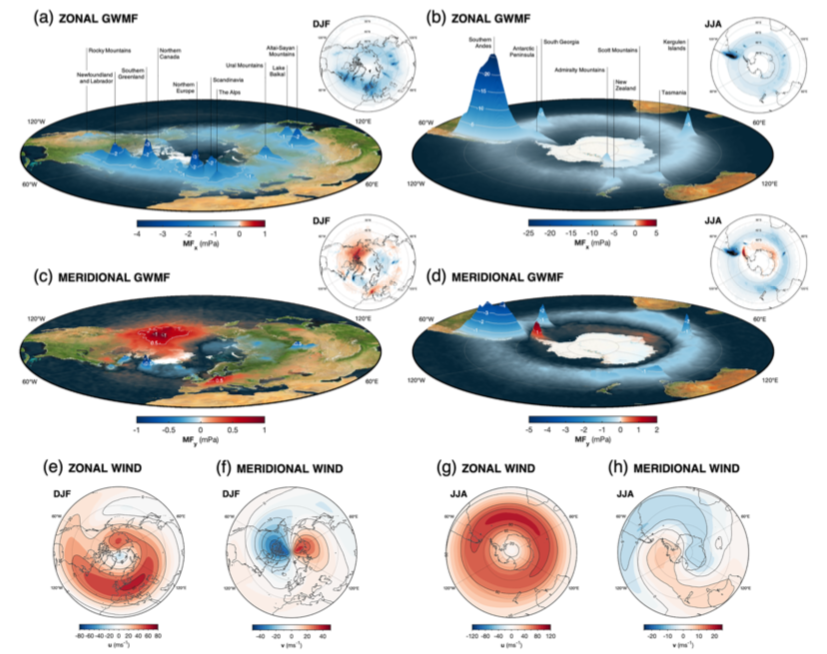
\includegraphics[width=0.85\textwidth]{figures_intro/hindley_2020_GWMF.png}
    \caption{Stereographic maps of average wintertime zonal (a, b) and meridional (c, d) GWMF near \SI{40}{\kilo\meter} altitude derived from AIRS/Aqua 3D satellite observations for the period 2002-2019. Winter is defined from December to February (June to August) for the Northern (Southern) Hemisphere. Gravity wave momentum flux values that are close to zero have been made transparent to reveal the surface features below, and landmarks that lie beneath regions of increased GWMF have been labeled. Inset in the top right of each panel is a stereographic map of the same data but centered on the north and south poles. These inset panels share a color scale with the corresponding 3D contours. Panels (e)-(h) show average wintertime zonal and meridional winds at 3 hPa for the period 2002-2019 from ERA5 reanalysis. Figure is taken from \cite{hindley_18year_2020}.}
    % Panels (e)–(h) show average wintertime zonal and meridional winds at 3 hPa for the period 2002–2019 from ERA5 reanalysis.
    \label{fig:hindley_2020_GWMF}
    %% change figure to southern hemisphere and include observational filter, then state ern 2018 observational filter better for shorter vertical wavelengths still observe GW belt (hindley discusses this in 2019 paper!!!!
    %Stratospheric zonal and meridional GWMF are illustrated on top of a map of the southern hemisphere. GWMF is derived from Atmospheric Infrared Sounder (AIRS) measurements between 2002 and 2019. Illustrated is the average over the austral winter months June – August. The figure is taken from Hindley et al. (2020))
\end{figure*}
%
The increasing number of GW observations from satellites (\cite{hindley_gravity_2019}, \citeyear{hindley_18year_2020}), ground-based lidar systems (\cite{kaifler_lidar_2020} and  \cite{kaifler_compact_2021}), aircraft (\cite{rapp_southtrac-gw_2021} and \cite{fritts_deep_2016}) and  balloons (\cite{plougonven_gravity_2013}) help to constrain GW parameterisations, but also reveal their deficiencies and point out gaps in our current theoretical knowledge on GWs. A phenomenon that was already visible in observations by \textcite{wu_satellite_1996}, but still lacks a conclusive explanation, is a GW belt around $60 \degree$S during the austral winter. It is illustrated in parts (b) and (d) of Figure \ref{fig:hindley_2020_GWMF} from \textcite{hindley_18year_2020}, who provide an extensive overview on seasonally averaged multi-year gravity wave momentum flux (GWMF) derived from satellite observations. \\
Orography undoubtedly leads to the GW hot spot between $55 \degree$W and $80 \degree$W above the southern Andes and the Antarctic Peninsula, but it only contributes about $25 \%$ to the total GWMF within the latitude band from $35 \degree$S to $68 \degree$S as stated by \textcite{hindley_18year_2020}. Following \textcite{sato_gravity_2012} and accounting for a far downstream propagation of GWs excited by the Andes, the observable GWMF in the East of the defined longitude region could be allocated to this predominantly local source, too. However, this does not heavily affect the argument of \textcite{hindley_18year_2020} that about $75 \%$ of zonal and meridional GWMF are observed at remaining longitudes over the Southern Ocean mostly peaking around $60 \degree$S (\cite{hindley_18year_2020}). \\
It has been shown that small, mountainous islands contribute to this oceanic GWMF (\cite{garfinkel_effect_2018}; \cite{mclandress_is_2012}, \cite{alexander_momentum_2009}), but again they only result in local peaks as indicated in Fig. \ref{fig:hindley_2020_GWMF}b. So non-orographic origins of GWs are most likely the reason for the wide-spread, belt-like structure of the GWMF (\cite{hendricks_what_2014}). Jet streams and fronts most likely contribute to the observed momentum flux (\cite{plougonven_internal_2014} and \cite{hendricks_what_2014}) and have also been investigated on the basis of idealized simulations (\cite{osullivan_generation_1995}). \textcite{polichtchouk_sensitivity_2018} analysed the sensitivity of high-resolution atmospheric models to non-orographic GW parameterisations and concluded a significant dependence in the same manner as \textcite{choi_effects_2013} showed that convective gravity wave drag parameterisations (a specific non-orographic source) can have a significant influence on global climate models. In addition, \textcite{jewtoukoff_comparison_2015} were able to assign wave signatures in their balloon observations to non-orographic sources, but so far none of the discussed mechanisms provides a comprehensive explanation of the wide spread observation of GWs over the Southern Ocean in the austral winter and it is still possible that some important mechanisms have not yet been considered.

The gravity wave belt around 60$\degree$S gained crucial relevance since \textcite{mclandress_is_2012} suggested its connection to the longstanding cold pole problem found in nearly all modern GCMs and chemistry climate models (CCMs). During the southern hemisphere winter months a polar vortex or polar night jet (PNJ) develops around 60$\degree$S high up in the stratosphere characterized by strong zonal westerly winds. GCMs and CCMs overestimate this PNJ, which also entails lower stratospheric temperatures over the pole compared to observations (\cite{butchart_multimodel_2011}, \cite{geller_comparison_2013} and \cite{eyring_sparc_2010}). As a result, the polar vortex breaks down too late in the spring with significant consequences on, for example, the simulated ozone trends in the Antarctic middle stratosphere (\cite{stolarski_ozone_2006}). The Antarctic ozone hole persists too long into the late spring and since Antarctic ozone depletion is the primary driver of recent southern hemisphere summertime climate change (e.g. \cite{arblaster_contributions_2006}), a delay in the vortex breakdown impacts the timing of the simulated tropospheric response. \\
\textcite{mclandress_is_2012} showed through their simulations that missing gravity wave drag from parameterisations can explain this substantial zonal wind bias around 60°S and the directly related "cold pole". A deeper understanding of the key processes that lead to the observed gravity wave belt during the austral winter could significantly improve GW parameterisations and ultimately improve long-term climate predictions through more realistic and robust GCMs. 

% include polar vortex image to show zonal wind distribution.

% or if it ultimately is a superposition of all known sources.

% temperature measurements of satellite
% in the vicinity of the 60°S belt

\section{The excitation of GWs above tropopause depressions}
\label{sec:excitation}
As outlined in the previous section, non-orographic GW sources have already been investigated from various perspectives, but are not yet able to fully explain the consistent, wide-spread appearance of GWs around 60$\degree$S. Based on observations and the analysis of high-resolution ERA5 data, \textcite{dornbrack_stratospheric_2022} propose a new mechanism that has the potential to fill this gap. They suggest an excitation of GWs above propagating tropopause depressions (TDs) in the stratosphere similar to the excitation of GWs above surface obstacles in the troposphere.

Though various definitions of the tropopause exist, all rely on abrupt changes in physical or chemical properties when transitioning from a weakly stratified troposphere ($N^2 \approx \SI{1e-4}{s^{-2}}$) to a strongly stratified stratosphere ($N^2 \approx \SI{4e-4}{s^{-2}}$) (\cite{birner_fine-scale_2006}). Common definitions are based on the thermal stratification (negative temperature lapse rate in the troposphere, positive  lapse rate in the stratosphere; \cite{wmo_meteorology_1957}), refer to the dynamical tropopause using Ertel's potential vorticity (\cite{wmo_atmospheric_1986}) or rely on chemical tracers like ozone. Despite fundamental differences in those approaches, each supports the simplification of treating the tropopause as an impermeable boundary, which is definitely not true, but a good approximation for idealized investigations. 

In the vicinity of jet streams or upper level frontal zones and associated with baroclinic processes the extratropical tropopause experiences deflections or even undergoes a folding process as visualized in Fig. \ref{fig:skerlakFold}. Dry stratospheric air penetrates down into the troposphere and folds underneath the warm air towards the equator (here northward for southern hemisphere) for deep depressions. % Potentially warmer stratospheric air
%
\begin{figure*}[t]
    \centering
    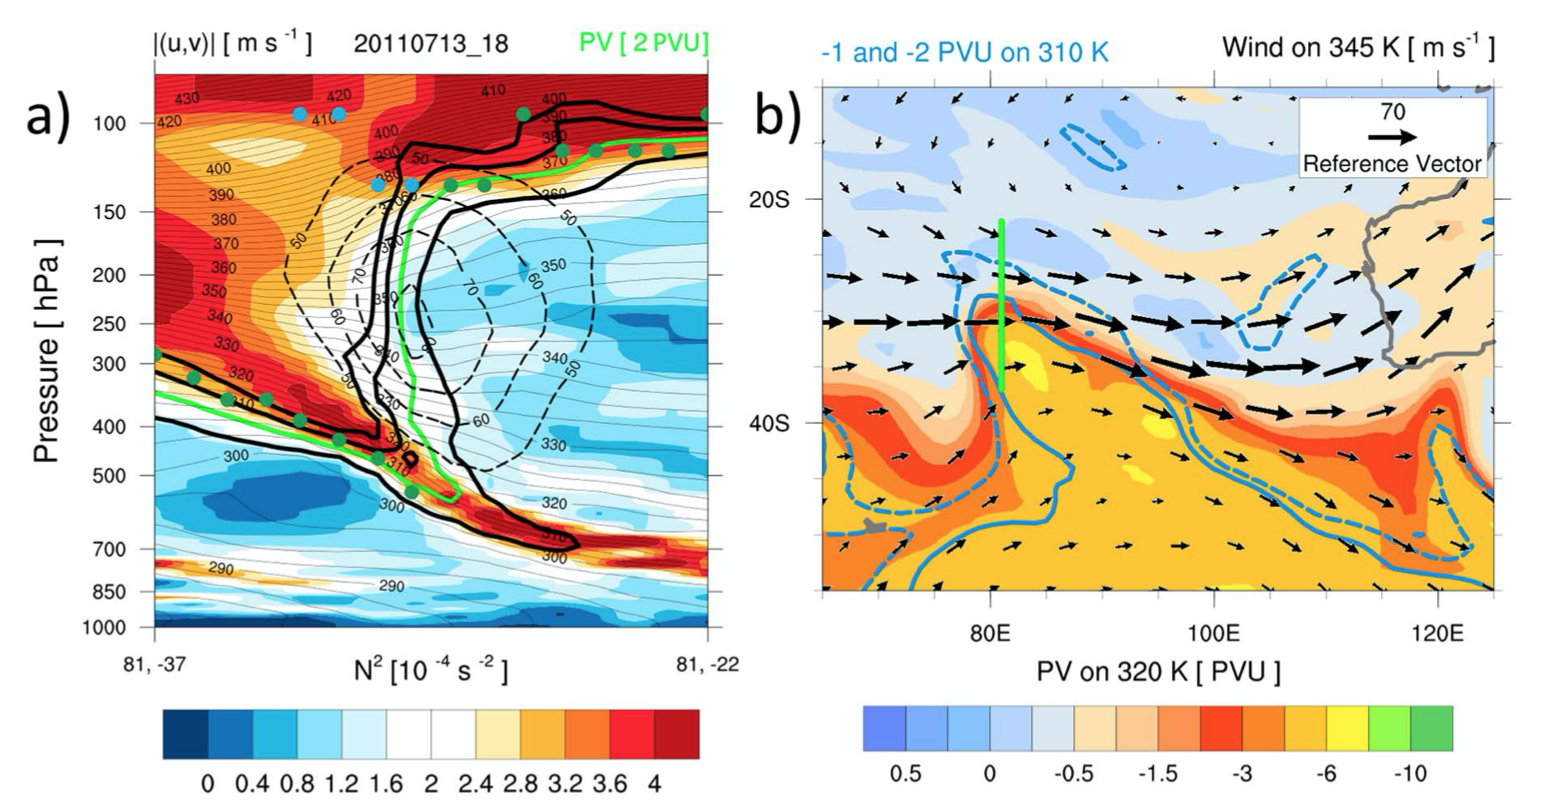
\includegraphics[width=0.9\textwidth]{figures_intro/Skerlak_Fold.png}
    \caption{Example of a deep tropopause fold near the subtropical jet west of Australia at 18 UTC on 13 July 2011. The vertical cross section shown in Figure 2a is aligned along 81$\degree$E from 37S$\degree$ to 22$\degree$S (green line segment in Figure 2b). Displayed are (a) the squared Brunt-Vaisala frequency ($N^2$, colored), potential vorticity (-1 to -4 PVU, thick solid lines, -2 PVU in green, rest in black), the WMO first and second tropopauses (green and blue solid circles, respectively), horizontal wind speed (in \SI{1}{\meter\second^{-1}}, dashed contours), and isentropes (in K, thin contours) and (b) PV on 320 K (colored, in PVU), contours of PV on 310 K at -1 PVU and -2 PVU (dashed and solid blue, respectively), and horizontal wind speed on 345K (reference vector in the top right, in \SI{1}{\meter\second^{-1}}). The West Coast of Australia is visible as grey contour. Taken from \cite{skerlak_tropopause_2015}.}
    \label{fig:skerlakFold}
\end{figure*}
%
The shape of the TD and especially the vertical extend of the prominent tongue of stratospheric air can vary significantly depending on the large scale flow conditions and strength of the upper level frontal system. This has already been discussed extensively from an observational (e.g. \cite{shapiro_further_1978} and \cite{keyser_review_1986}) and model (\cite{skerlak_tropopause_2015}) perspective. \\
Fortunately, the excitation of GWs above such a depression might not be very sensitive to the fold's shape far below the tropopause. Isentropes, that are deflected downwards, but rise again on the other side of the depression (e.g. 360-\SI{390}{\kelvin} in Figure \ref{fig:skerlakFold}a) are the ones of interest for the proposed mechanism because they mimic the flow over orography, or more precisely a valley. In addition, the zonal shape of the depression is more important for the GW forcing. This along-stream cross section (orthogonal on Figure \ref{fig:skerlakFold}a) is rarely discussed in the literature, because the main folding process happens in the cross-stream direction. Consequently, an estimate of realistic dimensions is based on the ERA5 case study by \textcite{dornbrack_stratospheric_2022} and further ERA5 analyses of cases discussed in Chapter \ref{cha:lidar} (e.g. Figure \ref{fig:era5_2018}). \textcite{dornbrack_stratospheric_2022} indicates the zonal shape of the investigated tropopause fold during their measurement campaign in the lower plots of Figure \ref{fig:RF25_era5_vertical}. The zonal width at half maximum of the propagating TD, and specifically of continuous isentropes above the tropopause, are estimated between $4 \degree$ and $12 \degree$, which transfers to a width of $240-$\SI{720}{\kilo\meter} ($1\degree \approx$ \SI{63}{\kilo\meter} at $55 \degree$S). \\
In an idealized scenario with constant background wind $U$ and Brunt–Väisälä frequency $N$ such "mountain widths" would be expected to excite waves within the hydrostatic and rotating wave regime. The advection time for an air parcel to pass over the mountain $\tau_a = \frac{a}{U}$ is comparable in magnitude to the period of inertial oscillation due to Earth’s rotation ($\tau_f = \frac{2 \pi}{f}$) with the Coriolis parameter $f \approx 10^{-4}$\SI{}{\second^{-1}} for mid-latitudes. So the Rossby number
% Thus, the time it takes for a fluid particle to cross the ridge is much larger than the period of a buoyancy oscillation
% We notice that τf /τa = 2πU/(fa) ≈ Ro
\begin{equation}
    Ro = \frac{U}{f a} \approx \frac{\tau_f}{\tau_a} \approx 2 \pi
\end{equation}
%
is close to $O(1)$ and Coriolis forces can no longer be neglected. Together with the buoyancy forces they act together as restoring forces resulting in both horizontal and vertical oscillations, which are called hydrostatic inertia-gravity waves (IGWs) (e.g. \cite{gill_atmosphere-ocean_1982} and \cite{lin_mesoscale_2007}).
% Froude number for linear non-linearity with height!!
% $L N U^{-1}$
% should be 60 m/s wind or 100km wide depression for hydrostatic scenario

A major difference of NOGWs above TDs to classic mountain waves is the transient nature of their source. \textcite{pfister_gravity_1993} already investigated the propagation of waves in the stratosphere due to a transient forcing by exposing the background flow to a time-varying obstacle, but only lifted and receded the bottom of the stratosphere. Here, a tropopause fold travels eastward with the phase speed of the Rossby wave, so the relative motion of the stratospheric air aloft to the depression's propagation speed is responsible for the excitation of the GWs. In other words, the propagating TD acts like an obstacle to the seasonally much faster stratospheric flow above. Consequently, the strong zonal winds in the stratosphere due to the PNJ during austral winter can be interpreted as a prerequisite for the excitation of NOGWs above tropopause depressions. During austral summer winds in the stratosphere are too weak and the excitation of such GWs is suppressed. \\
Simulations conducted by \textcite[]{prusa_propagation_1996} and \textcite[]{prusa_all-scale_2003} with a transient and horizontally moving lower boundary that mimics the tropopause went into that direction, but they focused on different aspects in a 2D plane. We follow a similar approach and focus on simulations of the stratosphere with the tropopause as a frictionless, impermeable lower boundary and stick to full 3D simulations to correctly represent IGWs with vertical and meridional oscillations. 

\section{The propagation of GWs above tropopause depressions}
\label{sec:propagation}
Considering the hydrostatic nature of GWs excited by TDs, the strongest wave signal should more or less appear directly above a propagating depression. And in fact, \textcite{dornbrack_stratospheric_2022} observed exactly this feature in ERA5 data, when analysing lidar measurements from the DEEPWAVE research flight 25. In Figure \ref{fig:RF25_era5_vertical}, clear wave signals mimic the appearance of MWs by leaning into the westerly wind and steepening in the positive shear of the PNJ. They are observed directly above the tropopause fold for the timestamps visualized and for the whole time series between them. This builds up confidence in the proposed mechanism of a "moving valley" and suggests that GWs can be observed along the whole path of a baroclinic system responsible for a TD. \\
%
\begin{figure*}[t]
    \centering
    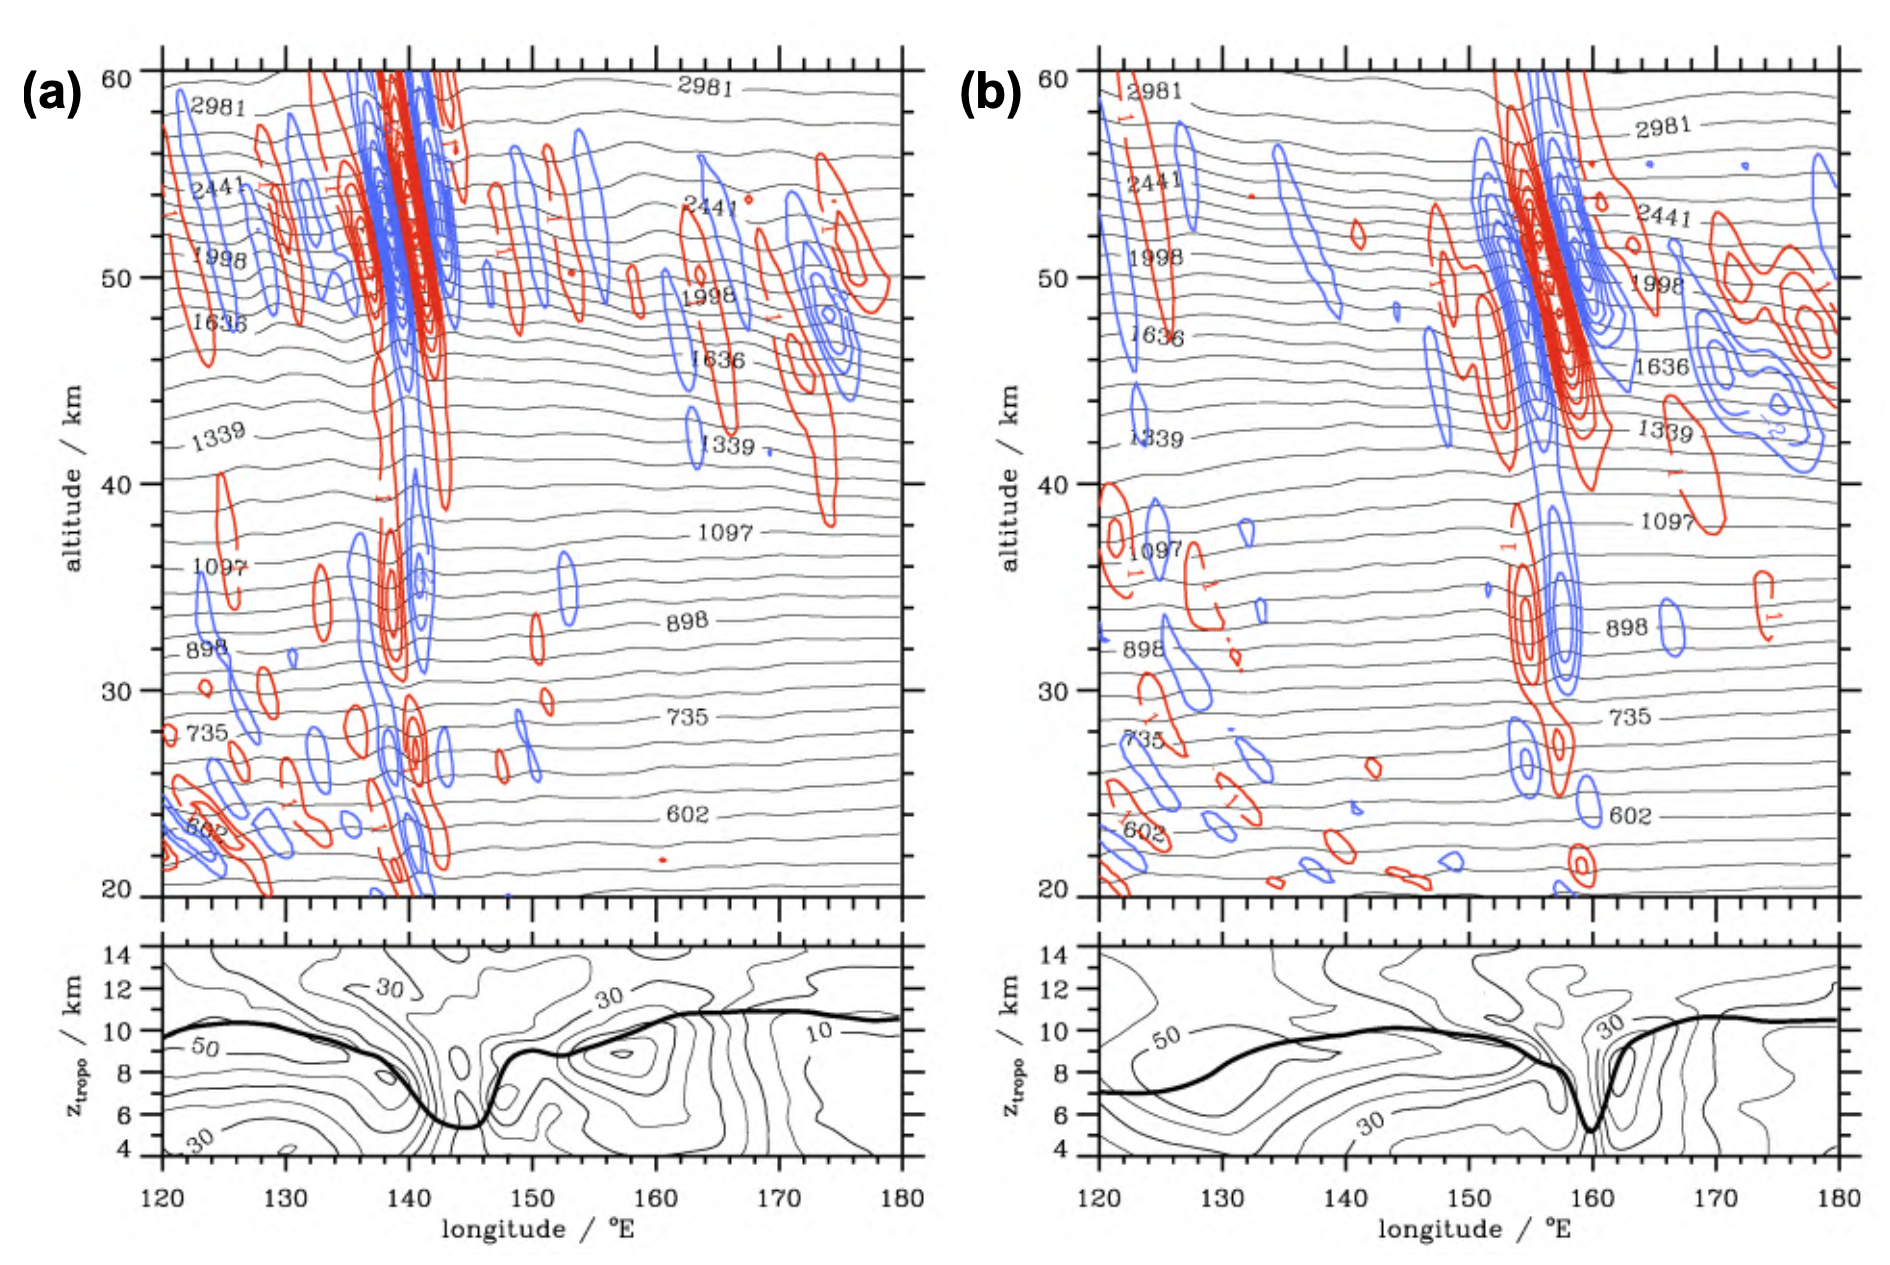
\includegraphics[width=0.99\textwidth]{figures_intro/RF25_ERA5_vertical.png}
    \caption{Temperature perturbations (K, red and blue contour lines) and potential temperature (K, black lines in logarithmic scaling) along 55$\degree$S on 17 July 2014 15 UTC (a) and 18 July 2014 09 UTC (b). The bottom panels depict the height of the dynamical tropopause (thick black lines, meridional average from 52.5$\degree$S to 57.5$\degree$S) and the horizontal wind (\SI{}{\meter\second^{-1}}, thin black lines) at the same instances. Data: One hourly ERA5 data. Taken from \textcite[]{dornbrack_stratospheric_2022}.}
    \label{fig:RF25_era5_vertical}
\end{figure*}
\begin{figure*}[t]
    \centering
    \includegraphics[width=0.99\textwidth]{figures_intro/RF25_ERA5_horizontal.png}
    \caption{Temperature perturbations $T'$ (K, color shaded) and geopotential height z (m, burgundy solid lines) at (a) 1, (b) 5, (c) 10, and (d) \SI{30}{hPa} at \SI{0900}{UTC} 18 Jul 2014. Data: ERA5 on a 0.28125° regular latitude-longitude grid. Taken from \textcite[]{dornbrack_stratospheric_2022}.}
    \label{fig:RF25_era5_horizonal}
\end{figure*} 
At this point, we note that pronounced baroclinic or frontal systems with tropopause folds in the southern hemisphere are not deviating significantly from a latitude band between 30-55$\degree$S (\cite{skerlak_tropopause_2015}). So how can NOGWs above these propagating tropopause folds explain the wave belt above the Southern Ocean centered further south at approximately 60°S in Figure \ref{fig:hindley_2020_GWMF}b and \ref{fig:hindley_2020_GWMF}d? The last piece to the puzzle is the meridional propagation of GWs in the stratosphere. \\
Two mechanisms can cause such a meridional propagation. At first, the orientation of the TDs is rarely north-south resulting in a slightly inclined wave vector with respect to the predominantly westerly flow in the upper stratosphere. The wave vector ($k$,$l$) defines the wave's intrinsic propagation direction and leads to a lateral deflection as soon as tilted obstacles with respect to the background flow are in place. \textcite{preusse_space-based_2002} for example considers this mechanism for GWs excited by the Andes at similar latitudes. The second process is based on ray-tracing theory and was first discussed and applied by \textcite{dunkerton_inertiagravity_1984}. It describes the modification of the meridional wavenumber by the background wind with
\begin{equation}
    \frac{dl}{dt} = -(k \frac{\partial U}{\partial y} + l \frac{\partial V}{\partial y} + \frac{\beta f}{\hat{\omega}})
    \approx -k \frac{\partial U}{\partial y}.
    \label{equ:meridionalRefraction}
\end{equation}
In a simplified scenario with purely zonal background flow ($V=0$) and no gradient of the Coriolis force $f$ ($\beta=0$), $\frac{dl}{dt}$ along the ray is proportional to the meridional gradient of the background wind $U$ and the zonal wavenumber $k$. In other words, meridional wind shear develops a meridional component of the wave vector even in the case of a purely zonal initial propagation. In general, this phenomenon leads to a refraction of internal GWs into the southern hemispheric PNJ at 60$\degree$S illustrated in Figure \ref{fig:hindley_2020_GWMF}g. It has already been described by a number of publications (e.g. \cite{dunkerton_inertiagravity_1984}, \cite{preusse_space-based_2002}, \cite{sato_origins_2009}, \cite*{sato_gravity_2012}, \cite{ehard_horizontal_2017} and \cite{jiang_stratospheric_2019}). \textcite{jiang_stratospheric_2019} further add, that waves are elongated towards the stronger background wind (towards the center of the PNJ) and shortened on the opposite side with weaker winds. \\
A zonally elongated GW pattern in the upper stratosphere is also present during the event in Figure \ref{fig:RF25_era5_vertical} by \textcite[]{dornbrack_stratospheric_2022}. Figure \ref{fig:RF25_era5_horizonal} shows corresponding horizontal cross sections at different pressure levels and at all heights phase lines have a very significant meridional wave vector component $l$. It seems that GWs are excited over the Southern Ocean somewhere southwest of Australia, then propagate up and south into the PNJ while getting refracted by the jet's shear. Especially at 1 and \SI{5}{hPa} in (a) and (b) the zonal extend of the elongated phase line pattern is very large, so one goal of this thesis will be a demonstration that NOGWs above tropopause folds can cause such a GW pattern within the southern hemisphere winter stratosphere.  

\section{Research goals and outline}
\label{sec:goals}
It is the overarching goal of this Master's thesis to take up the theories of \textcite[]{dornbrack_stratospheric_2022} and demonstrate that their proposed excitation mechanism of GWs above tropopause depressions can indeed explain individual observations of GWs in the upper stratosphere and contribute to the GW belt in the southern hemisphere winter stratosphere. Various different properties of the tropopause and the stratospheric environment will have a significant positive or negative influence on the excitation and propagation of these NOGWs, so a comprehensive sensitivity study based on idealized numerical simulations provides the basis for this investigation. In these simulations an impermeable, frictionless, transient lower boundary mimics the tropopause to simplify the simulation and focus on properties of the tropopause and on properties of the stratospheric environment. In a first step, we simplify even more and conduct computationally less expensive simulations with a coarse resolution in meridional direction and focus on zonal and vertical characteristics to answer our first research question in Chapter \ref{sec:resultsQ3D}.
\begin{tcolorbox}[]
    (R1) How sensitive are NOGWs from propagating tropopause depressions to the depression's 2D shape and to 2D properties of the stratospheric environment?
\end{tcolorbox}
Naturally, more complex simulations with an identical resolution in zonal and meridional direction follow in Chapter \ref{sec:results3D} and we can focus on meridional aspects of the tropopause and the meridional propagation of GWs within the stratosphere to answer the second research question of this thesis.
\begin{tcolorbox}[]
    (R2) How sensitive are NOGWs from propagating tropopause depressions to the depression's 3D shape and 3D properties of the stratospheric environment?
\end{tcolorbox}
The simulations in Chapter \ref{sec:results3D} also facilitate the investigation of the third research question, which refers to the zonally elongated phase lines in the horizontal cross sections of Figure \ref{fig:RF25_era5_horizonal}. As anticipated in the previous section, it is one goal of this thesis to check if the proposed excitation mechanism can also replicate the zonally elongated GW pattern (Figure \ref{fig:RF25_era5_horizonal}) in the stratosphere above the Southern Ocean described in the case study by \textcite[]{dornbrack_stratospheric_2022}. The third research question is also addressed in Chapter \ref{sec:results3D}. % and implies the identification of necessary properties to ob. 
\begin{tcolorbox}[]
    (R3) Can NOGWs above propagating tropopause depressions explain the zonally elongated phase lines in ERA5 above the Southern Ocean?
\end{tcolorbox} 
% Chapter 3 has comparison of momentum flux calculation from wind or temperature
The last research question links the idealized simulations of this thesis to available GW observations in the stratosphere, in particular, to ground-based lidar observations. Regular observations of GWs in this region are sparse, and for now, some ground-based lidar stations and the AIRS instrument onboard NASA's Aqua satellite are the only observations available regularly (\cite[]{kaifler_compact_2021} and \cite[]{hindley_18year_2020}). Ground-based lidar stations provide vertical timeseries with a high temporal and vertical resolution. These can also be emulated in the idealized numerical simulations to identify characteristics of GWs above propagating TDs that might allow a differentiation to other GWs like mountain waves. Research question four is addressed in Chapter \ref{cha:lidar}.
\begin{tcolorbox}[]
    (R4) Can NOGWs from propagating tropopause depressions be identified in lidar observations?
\end{tcolorbox}
We can anticipate that the propagating source of the GW implies a distinct pattern in vertical timeseries which opens the door to search for the respective pattern in actual measurements. Two observations of the Compact Rayleigh Autonomous Lidar (CORAL) currently located in Río Grande, Argentina at 53.79°S are also discussed in Chapter \ref{cha:lidar}.

A short overview on utilized tools and on the data is given in Chapter \ref{sec:methods} and the setup of all simulations is described in Chapter \ref{sec:EULAG}.

% INCLUDE OUTLOOK OF andreas paper with suggestions for further work

% Together with the regular appearance of Rossby wave trains (baroclinic systems involving TDs) at middle latitudes in the southern hemisphere, these processes could provide a conclusive explanation for the widespread and patchy stratospheric GW activity all the way around the Southern Ocean shown in Fig. \ref{fig:hindley_2020_GWMF}b and \ref{fig:hindley_2020_GWMF}d or in the case study in Figure ref{fig:RF25_era5_horizonal}. More specifically, the Master's thesis shall answer the following research questions:

%Figure \ref{fig:RF25_era5_vertical} was motivation for analogy of excitation mechanism with MWs, so this pattern is quite likely... however horizontal cross section pattern is interesting...


% Stationary synoptic patterns like blocks are rare in the southern hemisphere, because of 

% It is clear that the flow regime above a TD is much more complicated than a zonal overflow of an elongated mountain ridge, which produces the expected hydrostatic waves aloft. Three dimensional Furthermore, the fold itself travels eastward with the phase speed of the Rossby

% impermeable boundary
% shear wind rotation with height to strong zonal wind 

% The World Meteorological Organization defines the tropopause as the lowest level where the abso- lute value of the temperature lapse rate decreases to 2K/km. or less, with the average lapse rate between this level and all higher levels within 1.2 mi. (2 km.) not exceeding 2K/km. The dynamical tropopause is defined in terms of sharp changes in the potential vor- ticity (much higher in the stratosphere), which mea- sures stratification and rotation of the air masses. An abrupt increase (decrease) with height of the ozone (water vapor) mixing ratio indicates the presence of the chemical tropopause.

% thermal definition
% dynamic definition potential temperature and pressure on the dynamic tropopause (defined here as the 1.5 × 10−6 m2 K kg−1 s−1, hereafter 1.5 PVU, Ertel PV surface)
% chemical definition

% thermal fields and wind fields

% bush vertical / horizontal aspect ratio of 0.06 penetrates the troposphere

% \cite{clark_convectively_1986} above inversion layer?? 

% state that using tropopause fold and depression meaning the same

% half width is approximately 4/5 degree and 2 degree in zonal vertical cross section Dörnbrack et al

% Significant intrusions of stratospheric air occur in “ribbons” ~200 to 100 km in length, 100 to 300 km wide and about 1 to 4 km thick (EPA 2006).
\newpage
\thispagestyle{plain}

% ==== CHAPTER 2 ===============================================================
% ---- set some counters to zero:
\setcounter{equation}{0}
\setcounter{table}{0}
\setcounter{figure}{0}
% ---- include tex-file:
\chapter{Methods and data}
\label{sec:methods}
The following subsections provide a sufficient overview on the numerical model and analysis tools used for the presented work to allow a conclusive interpretation of the results thereafter.

\section{Spectral filtering}
\label{sec:spectral_filter}
% FFT

% and from Vera

- edge padding vs. symmetric padding. Pads with the reflection of the vector mirrored along the edge of the array.

- edge padding might overestimate changes in fluxes close to the surface.

- reflection / extension based on cutoff wavelength results in most realisitc estimation of fluxes 

- compare Gaussian filter vs. butterworth filter

- refer to filtering described in appendix of \textcite[]{kruse_gravity_2015}

- describe butterworth filter for CORAL data

\section{Wavelet Analysis}
\label{sec:wavelet}
The wavelet analysis described by \textcite{torrence_practical_1998} is used for deriving horizontal and vertical wavelengths of GWs in the idealized numerical simulations. 

% \begin{equation}
%     \mathcal{F}_x =  \rho_0 \int_{-\infty}^{\infty} (u'\omega' + f v' \eta') dx + f \int_{-\infty}^{\infty} \rho' v' \eta' dx
%     \label{equ:morlet}
% \end{equation}


- The normalization with the variance of the data $\sigma^2$ gives a measure of the power relative to white noise. 

- also describe red noise and Significance level

- 

\begin{figure*}[t]
    \centering
    \includegraphics[width=0.8\textwidth]{figures_methods/waveletAna_power_spectrum.png}
    \caption{}
    \label{fig:wavelet_example}
\end{figure*}


% Mithilfe der Wavelet-Transformation können aus einer Datenreihe nicht nur die auftre- tenden Frequenzen extrahiert werden, sondern auch Informationen darüber, in welchen Abschnitten der Datenreihe welche Frequenzen dominant sind. Als Basisfunktionen wer- den dabei räumlich lokalisierte Wellen, sogenannte Wavelets, verwendet.

% Folgenden wird die Wavelet-Analyse anhand einer Datenreihe f(z) erläutert, die ent- lang einer räumlichen Achse z variiert. Dabei wird auf die Beschreibung in Torrence & Compo (1998) zurück gegriffen. Die Autoren stellen auf der Website http://atoc.colorado.edu/research/wavelets/ Software zur Anwendung der Wavelet-Ana- lyse zur Verfügung, die in dieser Arbeit verwendet wurde.
% Hier wurde das Morlet-Wavelet ψ0(η) benutzt, das von einem dimensionslosen Ortspa- rameter η abhängt und als
% ψ0(η) = π−1/4 ei ω0η e−η2/2 (3.39)
% definiert ist. Real- und Imaginärteil von ψ0 sind in Abbildung 3.6a dargestellt. Wird f(z) als eine Datenreihe fj diskretisiert, die bei konstanter Intervallgröße ∆z auf einem Gitter mit Index j = 0,...,N−1 definiert ist, kann daraus die kontinuierliche Wavelet- Transformation Wn(s) ermittelt werden. Diese ist definiert als Faltung von fj mit einer skalierten und verschobenen Version der Wavelet-Funktion:
% N−1 Wj(s) = �� fj′ ψ∗
% ��(j′ −j)∆z�� s
% (3.40) die komplex konjugierte normierte Wavelet-Funktion ψ0.
%  Hierbei ist ψ
% ∗
% ���� ∆z ��1/2 ��∗ = s ψ0
% j′=0
%  Indem die Wavelet-Skala s variiert und ψ∗ entlang des Ortsindex j verschoben wird, kann ein Bild rekonstruiert werden, das sowohl die Amplitude einzelner Merkmale des Signals zeigt als auch die Variation der Amplitude mit dem Ort.
% Für jede Skala s muss Gleichung (3.40) N-mal angewandt werden, damit die kontinu- ierliche Wavelet-Transformation approximiert wird. Diese Berechnung erfolgt deutlich schneller im Fourier-Raum, wo die Wavelet-Transformation gleichzeitig für alle N durch- geführt werden kann. Für die Skalen s empfiehlt sich eine Wahl von M Skalen, die als Vielfache von 2 ausgedrückt werden:
% sm = s0 2m∆m mit m = 0,1,...,M und M = ∆m−1 log2(N ∆m/s0)
% Die kleinste Skala s0 sollte dabei so gewählt werden, dass die entsprechende Fourier-
% Periode etwa 2∆z beträgt. Aus der komplexen Wavelet-Transformierten Wj(s) kann
% das reelle Wavelet-Leistungsspektrum |Wj(s)| berechnet werden. Bei der Interpretation
% dieses Spektrums muss beachtet werden, dass bei der Fourier-Transformation eine An-
% nahme bezüglich zyklischer Daten gemacht wird, die nicht unbedingt erfüllt ist. An den
% Rändern des Datensatzes können deshalb Fehler auftreten. Der Einflusskegel (engl.: cone
% of influence) gibt an, in welchen Bereichen des Spektrums Randeffekte wichtig werden.
% Er ist definiert als e-Abklingzeit τs der Wavelet-Leistung zu jeder Skala s und für das √
% Morlet-Wavelet gilt τs = 2 s.
% Im rechten Bildteil von Abbildung 3.6c ist ein Wavelet-Leistungsspektrum dargestellt, in dem auch der Einflusskegel als weiße Linie markiert ist. Die schwarze Kontur gibt ein Konfidenzniveau von 95 % an, bezogen auf ein Spektrum roten Rauschens mit lag-

% 1-Koeffizient 0.72 (siehe Torrence & Compo, 1998). Es zeigt die Wavelet-Analyse ei- nes Profils des Vertikalwinds (mittlerer Bildteil von Abbildung 3.6c) aus einer EU- LAG-Simulation. Der Vertikalschnitt durch das Windfeld ist in Abbildung 3.6b als rot-gestrichelte Linie dargestellt. Im Wavelet-Leistungsspektrum, das mit dem Morlet- Wavelet (Abbildung 3.6a) erstellt wurde, können einzelne Bereiche als dominante Signale ausgemacht werden. Im unteren Bereich bis zu einer Höhe von z = 10 km ist eine ver- tikale Wellenlänge λz zwischen etwa 2 000 m und 3 000 m verstärkt vorhanden, während in größeren Höhen kleinere Wellenlängen von unter 1000m das Spektrum bestimmen. Dieser Fall ist in Abschnitt 4.2.1 ausführlich besprochen.


% include figure from wavelet analysis for one line in 2D data, show line in T' plot..

% Figure: wavelet + cut + power spectrum 


\section{CORAL temperature measurements} 
\label{sec:coral}

\textcite{kaifler_compact_2021} provide a more extensive summary on CORAL's setup and observation,


\section{(ERA5 reanalysis data)}

In Chapter \ref{cha:lidar} we use the ERA5 reanalysis introduced by \textcite[]{hersbach_era5_2020} for two case studies on GW observations by the ground-based lidar CORAL in Río Grande at the southern tip of south 
% Within the Copernicus Climate Change Service (C3S), ECMWF is producing the ERA5 reanalysis which, once completed, will embody a detailed record of the global atmosphere, land surface and ocean waves from 1950 onwards. This new reanalysis replaces the ERA-Interim reanalysis (spanning 1979 onwards) which was started in 2006. ERA5 is based on the Integrated Forecasting System (IFS) Cy41r2 which was operational in 2016. ERA5 thus benefits from a decade of developments in model physics, core dynamics and data assimilation. In addition to a significantly enhanced horizontal resolution of 31 km

Copernicus Climate Change Service (C3S) Climate Data Store (CDS)

cite Hersbach paper and ML dataset for temperature perturbations 

winds on 850hPa

and height of dynamical tropopause (2 PVU level)

and d
- maybe also comment on observational filter of satellite measurments from with figure from Hindley
\newpage
\thispagestyle{plain}

% ==== CHAPTER 3 ===============================================================
% ---- set some counters to zero:
\setcounter{equation}{0}
\setcounter{table}{0}
\setcounter{figure}{0}
% ---- include tex-file:
\chapter{The numerical model EULAG}
\label{sec:EULAG}
The nonlinear numerical simulations are conducted with the EUlerian/semi- LAGrangian fluid solver (EULAG). EULAG was written by Piotr Smolarkiewicz, but many others contributed to the code. The research code is comprised in one file combining two programming languages, shell script and FORTRAN (mostly FORTRAN 77), to create a very fast executable program. A comprehensive description of the algorithm is given in \textcite[]{smolarkiewicz_forward--time_1997} and \textcite[]{smolarkiewicz_mpdata_1998}. \\
EULAG has a proven itself as a reliable tool for simulating thermo-fluid flows across the wide range from turbulent to global scales (\cite{prusa_all-scale_2003}) and in a variety of physical scenarios like e.g. turbulence, GW dynamics, flows past complex/moving boundaries, micrometeorology or cloud microphysics (\cite{prusa_eulag_2008}). A comparison between different well-established numerical models (including EULAG) and their capability to model flow over steep terrain, which is relevant for the investigations within this thesis, appears in \textcite{doyle_intercomparison_2011}.

The underlying setup of EULAG for this work is described in the first section of this chapter \ref{sec:eulag-setup}. It follows a more detailed description of relevant atmospheric background conditions in section \ref{sec:ambient-profiles} and the implementation of a transient lower boundary for the idealized simulations is explained in section \ref{sec:trans-boundary}. Section \ref{sec:linear-MWs} completes this chapter with a comparison of non-linear EULAG simulations to analytic results from linear theory for different MW scenarios. It serves as an additional validation of EULAG before using it for the investigation of NOGWs above propagating tropopause folds.

%%%%%%%%%%%% General setup %%%%%%%%%%%%%%%%
\section{General setup}
\label{sec:eulag-setup}
The model is set up solving the soundproof anelastic set of equations (\cite{lipps_scale_1982}) consisting of the three components of the momentum equation (\ref{equ:momEqu}), the thermodynamic equation (\ref{equ:potTemp}) for the potential temperature perturbation $\Theta'=\Theta-\Theta_e$ and the mass continuity equation (\ref{equ:continuityEqu}):
%
\begin{equation}
\begin{aligned}
    \frac{d \Vec{v}}{dt} = -G \Vec{\nabla} \biggl(\frac{p'}{\rho_0}\biggr) +  \Vec{g} \frac{\Theta'}{\Theta_0} - 2 \Vec{\Omega} \times \bigl(\Vec{v}-\Vec{v_e}\bigr) - \Tilde{\alpha} \bigl(\Vec{v}-\Vec{v_e}\bigr) \equiv R^{v},
    \label{equ:momEqu}
\end{aligned}
\end{equation}
\begin{equation}
    \frac{d \Theta'}{dt} = -\Vec{v} \cdot \Vec{\nabla} \Theta_e - \Tilde{\beta} \bigl(\Theta-\Theta_e\bigr) \equiv R^{\Theta},
    \label{equ:potTemp}
\end{equation}
\begin{equation}
    \Vec{\nabla} \cdot \bigl(\rho_0 \Vec{v}\bigr) = 0.
    \label{equ:continuityEqu}
\end{equation}
%
Here, $\frac{d}{dt}$, $\Vec{\nabla}$ and $\Vec{\nabla} \cdot$ represent the total derivative, the gradient and the divergence respectively. $p'$ is the pressure perturbation with respect to the environmental state, g the gravitational acceleration and $\Vec{\Omega}$ the angular velocity of the Earth. The matrix G represents geometric terms, which result from the general, time-dependent coordinate transformation and the symbol $R^{\Psi}$ stands for the right-hand side of the corresponding equations for the variables $\Psi = (u,v,w,\Theta')$. \\
$\rho_0(z)$ and $\Theta_0(z)$ refer to the hydrostatic reference state or basic state of equations (\ref{equ:momEqu}-\ref{equ:continuityEqu}). EULAG provides multiple options to define this reference state of the atmosphere including one that is well suited for modelling deep atmospheres following \textcite{bacmeister_breakdown_1989}. A more general environmental state, which reflects the initial and boundary conditions, enters the equations via the variables with subscript e. These ambient states like $u_e$, $\rho_e$ or $\Theta_e$ can relate to the reference state, but they can also be time-dependent to replicate transient flow conditions. In that sense, $\alpha(\Vec{v}-\Vec{v_e})$ and $\beta(\theta-\theta_e)$ represent relaxation terms, which enable the radiation of wave energy across the model boundaries and force the solutions at the boundaries to the prescribed environmental profiles. Both, reference and environmental profiles are described in detail in the following section \ref{sec:ambient-profiles}. \\
A particularly useful feature of EULAG for our simulations is the possibility for transient boundaries (\cite[]{prusa_propagation_1996} and \cite{wedi_extending_2003}). We will use this option to mimic a propagating tropopause fold at the lower boundary and to avoid unphysical, transient processes during the initialization of the simulation. More details follow in section \ref{sec:trans-boundary}. Furthermore, EULAG is noteworthy for its robust elliptic solver (\cite{smolarkiewicz_forward--time_1993}) and generalized coordinate formulation enabling grid adaptivity technology (\cite{prusa_eulag_2008}, \cite{kuhnlein_modelling_2012}).

\subsection*{Numerics}
As the name suggests, EULAG is capable of solving the equations of motion (\ref{equ:momEqu}-\ref{equ:continuityEqu}) in an Eulerian (flux form) or in a semi-Lagrangian (advective form) mode (\cite{smolarkiewicz_forward--time_1997}). For the numerical approximation it utilizes a non-oscillatory forward-in-time (NFT) approach compactly formulated as
\begin{equation}
\begin{aligned}
    \Psi^{n+1} = LE(\Tilde{\Psi}, V^{n+1}, G^n, G^{n+1}) \\
    + \frac{1}{2} \Delta t R^{\Psi} |^{n+1}
    \label{equ:NFTscheme}
\end{aligned}
\end{equation}
with $LE$ representing the corresponding semi-Lagrangian/Eulerian transport operator. The NFT scheme belongs to the class of second-order-accurate two-time-level algorithms that are build on nonlinear advection techniques (\cite{prusa_eulag_2008}). These schemes have the property to suppress and control numerical oscillations that are often found in higher order linear schemes. As a result, transporting the auxiliary field $\Tilde{\Psi} = \Psi^n + \frac{1}{2} \Delta t R^{\Psi}|^n$ instead of the specific variable $\Psi$, results from a thorough truncation error analysis and ensures second order accuracy. (\cite{smolarkiewicz_forward--time_1997}). Within the scope of this Master's thesis all simulations utilize the Eulerian option by applying the multidimensional positive definite advection transport algorithm MPDATA (\cite{smolarkiewicz_mpdata_1998} and \cite{smolarkiewicz_multidimensional_2006}).

%%%%% NOTES %%%%%

% Prusa 2008 also has good description of perturbation form and points out importance of correct environmental/initial state!! 

% \cite{smolarkiewicz_multidimensional_2006}

% \begin{equation}
%    \frac{\partial G \rho \Psi}{\partial t} + \nabla \cdot G \rho \Vec{v} = G \rho R
%    \label{equ:statMeshAdapt}
% \end{equation}


% he elliptic pressure equation is solved via a preconditioned non-symmetric Krylov sub- space solver (Smolarkiewicz and Margolin; 1994; 1997, Skamarock et al., 1997).

% imlicit /explicit elliptic pressure solver / krylov sub space solver

% There, governing equations are formulated in general- ized time-dependent curvi-linear coordinates to enable mesh adaptivity (Prusa and Smolarkiewicz 2003; Wedi and Smolarkiewicz 2004; Kühnlein et al. 2012; Smolarkiewicz and Charbonneau 2013) and continuous mappings of the Earth’s topography by using terrain-following coordinates (Gal-Chen and Somerville 1975; Clark 1977)


% anelastic -> elastic energy is not allowed -> sound waves are filtered since they are based on pressure difference rather then temperature

%%%%%%%%%%%% Ambient profiles %%%%%%%%%%%%%%%%
\section{Ambient profiles of idealized simulations}
\subsection*{The hydrostatic reference state: Bacmeister-Schoeberl Model}
\begin{figure*}[tbp]
    \centering
    \includegraphics[width=0.45\textwidth]{figures_model/bac-schoeber-ambient-profiles.png}
    \caption{Vertical profiles of ambient pressure $p_0$ (orange), density $\rho_0$ (blue), absolute temperature $T_0$ (red) and potential temperature $\Theta_0$ (purple) scaled by corresponding surface values for the isothermal atmosphere described by \textcite[]{bacmeister_breakdown_1989}.}
    \label{fig:ambient_profs}
\end{figure*}
\label{sec:ambient-profiles}
The anelastic equations (\ref{equ:momEqu}-\ref{equ:continuityEqu}) rely on hydrostatically balanced reference profiles of the dependent variables ($\rho$, $p$ and $\Theta$) that vary with height, but not horizontally or in time. For the presented idealized simulations these reference profiles (subscript 0 in the previous section) define an isothermal atmosphere with constant stability following \textcite{bacmeister_breakdown_1989}. In the anelastic framework it is only necessary to define the vertical profile of potential temperature and a reference pressure $p_{00}$. All other variables follow from the definition of $\Theta$
\begin{equation}
    \Theta(z) = T(z) \biggl(\frac{p_{0}}{p}\biggr)^{\kappa},
    \label{equ:poissonEqu}
\end{equation}
the ideal gas law
\begin{equation}
    \rho(z) = \frac{p(z)}{R T(z)}
    \label{equ:idealGas}
\end{equation}
and the assumption of hydrostatic balance $\frac{dp}{dz}=-\rho g$ that results in
% general equation in 
\begin{equation}
    \frac{1}{\rho} \frac{d \rho}{dz} + \frac{1}{\Theta} \frac{d \Theta}{dz} = \frac{\kappa-1}{H_{\rho}} \biggl(\frac{\rho}{\rho_0} \biggr)^{\frac{\kappa}{\kappa-1}} \biggl(\frac{\Theta}{\Theta_0} \biggr)^{\frac{1}{\kappa-1}}
    \label{equ:hydro-balance}
\end{equation}
and can be solved for a density profile $\rho(z)$ after defining the potential temperature profile $\Theta(z)$. For the isothermal atmosphere of \textcite[]{bacmeister_breakdown_1989} it provides $H_{\rho} = \kappa H_{\Theta}$ and the reference profiles (Figure \ref{fig:ambient_profs})
\begin{equation}
    \begin{aligned}
        \Theta_0(z) &= T_{00} e^{\frac{z}{H_{\Theta}}} \quad \textrm{with} \quad H_{\Theta} = \frac{g}{N^2} = \frac{c_p T_{00}}{g}, \\
        \rho_0(z) &= \rho_{00} e^{-\frac{z}{H_{\rho}}} \quad \textrm{with} \quad H_{\rho} = \frac{R T_{00}}{g} \quad \textrm{and}  \\
        p_0(z) &= p_{00} e^{-\frac{z}{H_{\rho}}}
        \label{equ:ambient-profiles}
    \end{aligned}
\end{equation}
with the Brunt-Vaisala frequency $N=\bigl(\frac{g}{\Theta}\frac{\partial \bar{\Theta}}{\partial z}\bigr)^{\frac{1}{2}}$, the specific gas constant $R$ and the specific heat capacity at constant pressure $c_p$. These exponential profiles avoid physical restrictions towards higher altitudes (compare Figure \ref{fig:ambient_profs}) and are thus well suited for the investigation of deep gravity wave propagation. \\
All relevant parameters for these ambient profiles used for our simulations are summarized in Table \ref{tab:ambientProfiles}. Values for the troposphere are used for EULAG simulations of linear MW scenarios in section \ref{sec:linear-MWs}, values for the stratosphere are used for all simulations of a propagating tropopause fold in chapters \ref{sec:resultsQ3D} and \ref{sec:results3D}. The fact that there are two columns for the troposphere emphasizes a quite unrealistic relation of the isothermal temperature $T_{00}$ and $\kappa$ for a tropospheric Brunt-Väisälä frequency of $N=\SI{0.01}{\per\second}$. Based on the definition of $H_{\Theta}$ and $H_{\rho}$ choosing $\kappa=\frac{2}{7}$ to represent diatomic gases results in a very high temperature $T_{00} = \SI{957}{K}$. For a more realistic temperature $T_{00} = \SI{274}{K}$ $\kappa$ has to be reduced to $\kappa=\frac{2}{24.4}$. When using the soundproof anelastic equations similar to \textcite[]{lipps_scale_1982} the choice of $\kappa$ and $T_{00}$ is not affecting energy and momentum fluxes, so both descriptions of the troposhere in Table \ref{tab:ambientProfiles} lead to the same result in section \ref{sec:linear-MWs}. This has been tested, too. For simulations of the stratosphere with $N=\SI{0.02}{\per\second}$ a $\kappa$ for diatomic gases leads to a reasonable temperature of $T_{00} = \SI{239}{K}$.
\begin{table*}[ht]
\centering
\caption{Summary of parameters related to the vertical profiles of the ambient reference state following \textcite[]{bacmeister_breakdown_1989}. Values for the troposphere are used for the model validation in section \ref{sec:linear-MWs}. Values for the stratosphere are used for simulations of a propagating tropopause fold in chapters \ref{sec:resultsQ3D} and \ref{sec:results3D}. The first troposphere column is for a reasonable temperature $T_{00}$, the second troposphere column is for a diatomic gas. Grey rows refer to parameters that need to be defined.}
\begin{tabular}{@{}ccccc@{}}
\toprule
 & Unit & Troposphere & Troposphere ($\kappa=\frac{2}{7}$) & Stratosphere \\ \midrule[1pt]

 \rowcolor{LightCyan} $R$ & J kg$^{-1}$ K$^{-1}$ &   \cellcolor{LightCyan} 287.04 &   \cellcolor{LightCyan} 287.04 &   \cellcolor{LightCyan} 287.04 \\
 \rowcolor{LightCyan} $g$ & m s$^{-2}$ & \cellcolor{LightCyan} 9.80616 & \cellcolor{LightCyan} 9.80616 & \cellcolor{LightCyan} 9.80616 \\
 \rowcolor{LightCyan} $N$ & s$^{-1}$ & \cellcolor{LightCyan} 0.01 & \cellcolor{LightCyan} 0.01 & \cellcolor{LightCyan} 0.02 \\
\rowcolor{LightCyan} $\kappa$ & - & $\frac{2}{24.4}$ & $ \frac{2}{7}$ & $ \frac{2}{7}$ \\
$c_p$ & J kg$^{-1}$ K$^{-1}$ & $\frac{24.4}{2} R$ & $\frac{7}{2} R$ & $\frac{7}{2} R$ \\
$H_{\Theta}$ & m & 98061.6 & 98061.6 & 24515.4  \\
$H_{\rho}$ & m & 8011.3  & 28017.6  & 7004.4 \\

& & & & \\
\rowcolor{LightCyan} $p_{00}$ & Pa & \cellcolor{LightCyan} $1.01 \times 10^5$ & \cellcolor{LightCyan} $1.01 \times 10^5$ & \cellcolor{LightCyan} $0.235 \times 10^5$ \\
$T_{00}$ & K & 273.69 & 957.17 & 239.39 \\
$\rho_{00}$ & kg m$^{-3}$ & 1.2856 & 0.3676 & 0.3454 \\

\bottomrule
\end{tabular}
\label{tab:ambientProfiles}
\end{table*}

Ambient profiles (subscript $e$ in the anelastic equations (\ref{equ:momEqu}-\ref{equ:continuityEqu})) of the dependent variables ($\rho_e$, $p_e$ and $\Theta_e$) are stationary (not time-dependent) and therefore identical to the vertical profiles of the hydrostatic reference state (subscript 0).

\subsection*{Ambient wind profiles}
All presented simulations are conducted in 3D, but enforce a purely zonal background flow $u_e(z,y)$ with no meridional background wind $v_e=0$. Nevertheless, meridional perturbations $v'$ develop due to the Coriolis force and the 3D nature of inertia-gravity waves. Some simulations including the model validation in section \ref{sec:linear-MWs} have a constant wind $u_e$ without vertical and meridional shear. In the remaining simulations for the sensitivity study in chapter \ref{sec:resultsQ3D} $u_e(z)$ varies with altitude, but it is still constant in meridional direction. In chapter \ref{sec:results3D} $u_e(z,y)$ is a function of $z$ and $y$ to incorporate the meridional structure of the PNJ. At this point, it is important to note that vertical gradients of the zonal background wind $u_e$ are not coupled to meridional gradients of $\Theta_e$ and $\frac{\partial \Theta_e}{\partial y}=0$ for all simulations. Winds are independent of the potential temperature distribution and in the case of $\frac{\partial u_e}{\partial z} \neq 0$ the thermal wind relation is not fullfilled. Considering the thermal wind relation and simulating a baroclinic instability at tropopause level would be the next step as proposed in the outlook.

\begin{figure*}[tbp]
    \centering
    \includegraphics[width=0.67\textwidth]{figures_model/era5-winds-reichert.png}
    \caption{Illustrated are ERA5 monthly mean absolute wind profiles (thick lines, lower axis) and wind directions above Río Grande (thin lines, upper axis; the dashed lines mark westerlies). The wind field was truncated at T21 in order to filter out contributions from model-resolved GWs. Winter months in the southern hemisphere are blue, summer months red. are The figure is taken from \textcite[]{reichert_characterization_2022}.}
    \label{fig:era5-winds-reichert}
\end{figure*} 
% \cite[]{hindley_radar_2022}
The goal for our simulations was an idealized wind profile typical for the southern hemisphere winter stratosphere with features that can be adjusted individually for a conclusive sensitivity study. A good source of information for the construction of $u_e$ was Figure \ref{fig:era5-winds-reichert} from \textcite[]{reichert_characterization_2022} who analysed monthly means of ERA5 winds above Río Grande at the southern tip of South America (\SI{53.79}{\degree S}) for the years 2017 to 2020. Other sources based on ERA5 data were \textcite[]{rapp_southtrac-gw_2021}, \textcite[]{mixa_nonlinear_2021} and \textcite[]{dornbrack_stratospheric_2022} who also showed profiles from radiosondes and the IFS model (ECMWF) for their case study in the appendix. \\
All show a clear vertical pattern for the winter stratosphere between 50-\SI{60}{\degree S} with a local maximum around the tropopause at 8-\SI{10}{\kilo\meter} (tropopause jet) and a much stronger PNJ at approximately 35-\SI{45}{\kilo\meter} above the tropopause. In most cases, a wind minimum exists above the tropopause jet at approximately 15-\SI{20}{\kilo\meter} (e.g. APR or MAY in Figure \ref{fig:era5-winds-reichert}). This minimum can be more or less pronounced and even vanish (e.g. AUG and SEP for the years 2018 and 2020 in Figure \ref{fig:era5-winds-reichert}) resulting in positive vertical shear throughout the whole stratosphere. Wind maxima of the tropopause jet mostly vary between 35-\SI{55}{\meter\per\second}. The PNJ reaches wind speeds from 60-\SI{140}{\meter\per\second}. \\
To consider and vary these different features independently the idealized vertical profile $u_e(z)$ is a superposition of a base wind U$_0$ and two jet streams (Figure \ref{fig:wind_profs}a) that are both based on a Gaussian distribution
\begin{equation}
    u_e(z) = u_{jet,max} e^{-\frac{1}{2} \bigl(\frac{z-z_{jet}}{\sigma_{jet}}\bigr)^2}
    \label{equ:wind-distribution}
    % squared for symmetric distribution
\end{equation}
with a maximum wind speed $u_{jet,max}$ at $z_{jet}$ and a standard deviation $\sigma_{jet}$ to adjust the vertical gradient $\frac{\partial u_e}{\partial z}$ by making the distribution wider or narrower. In Figure \ref{fig:wind_profs}a the tropopause jet TPJ (purple dashed line) is centered at the lower boundary of the simulation with $\sigma_{jet}=\SI{5}{\kilo\meter}$ and the PNJ (yellow dashed line) is centered at $z_{jet}=\SI{40}{\kilo\meter}$ with $\sigma_{jet}=\SI{13}{\kilo\meter}$. Different parameter combinations result in different vertical profiles of $u_e$, which are compared in section \ref{sec:q3D-wind} and Figure \ref{fig:q3D_wind}.

\begin{figure*}[tbp]
    \centering
    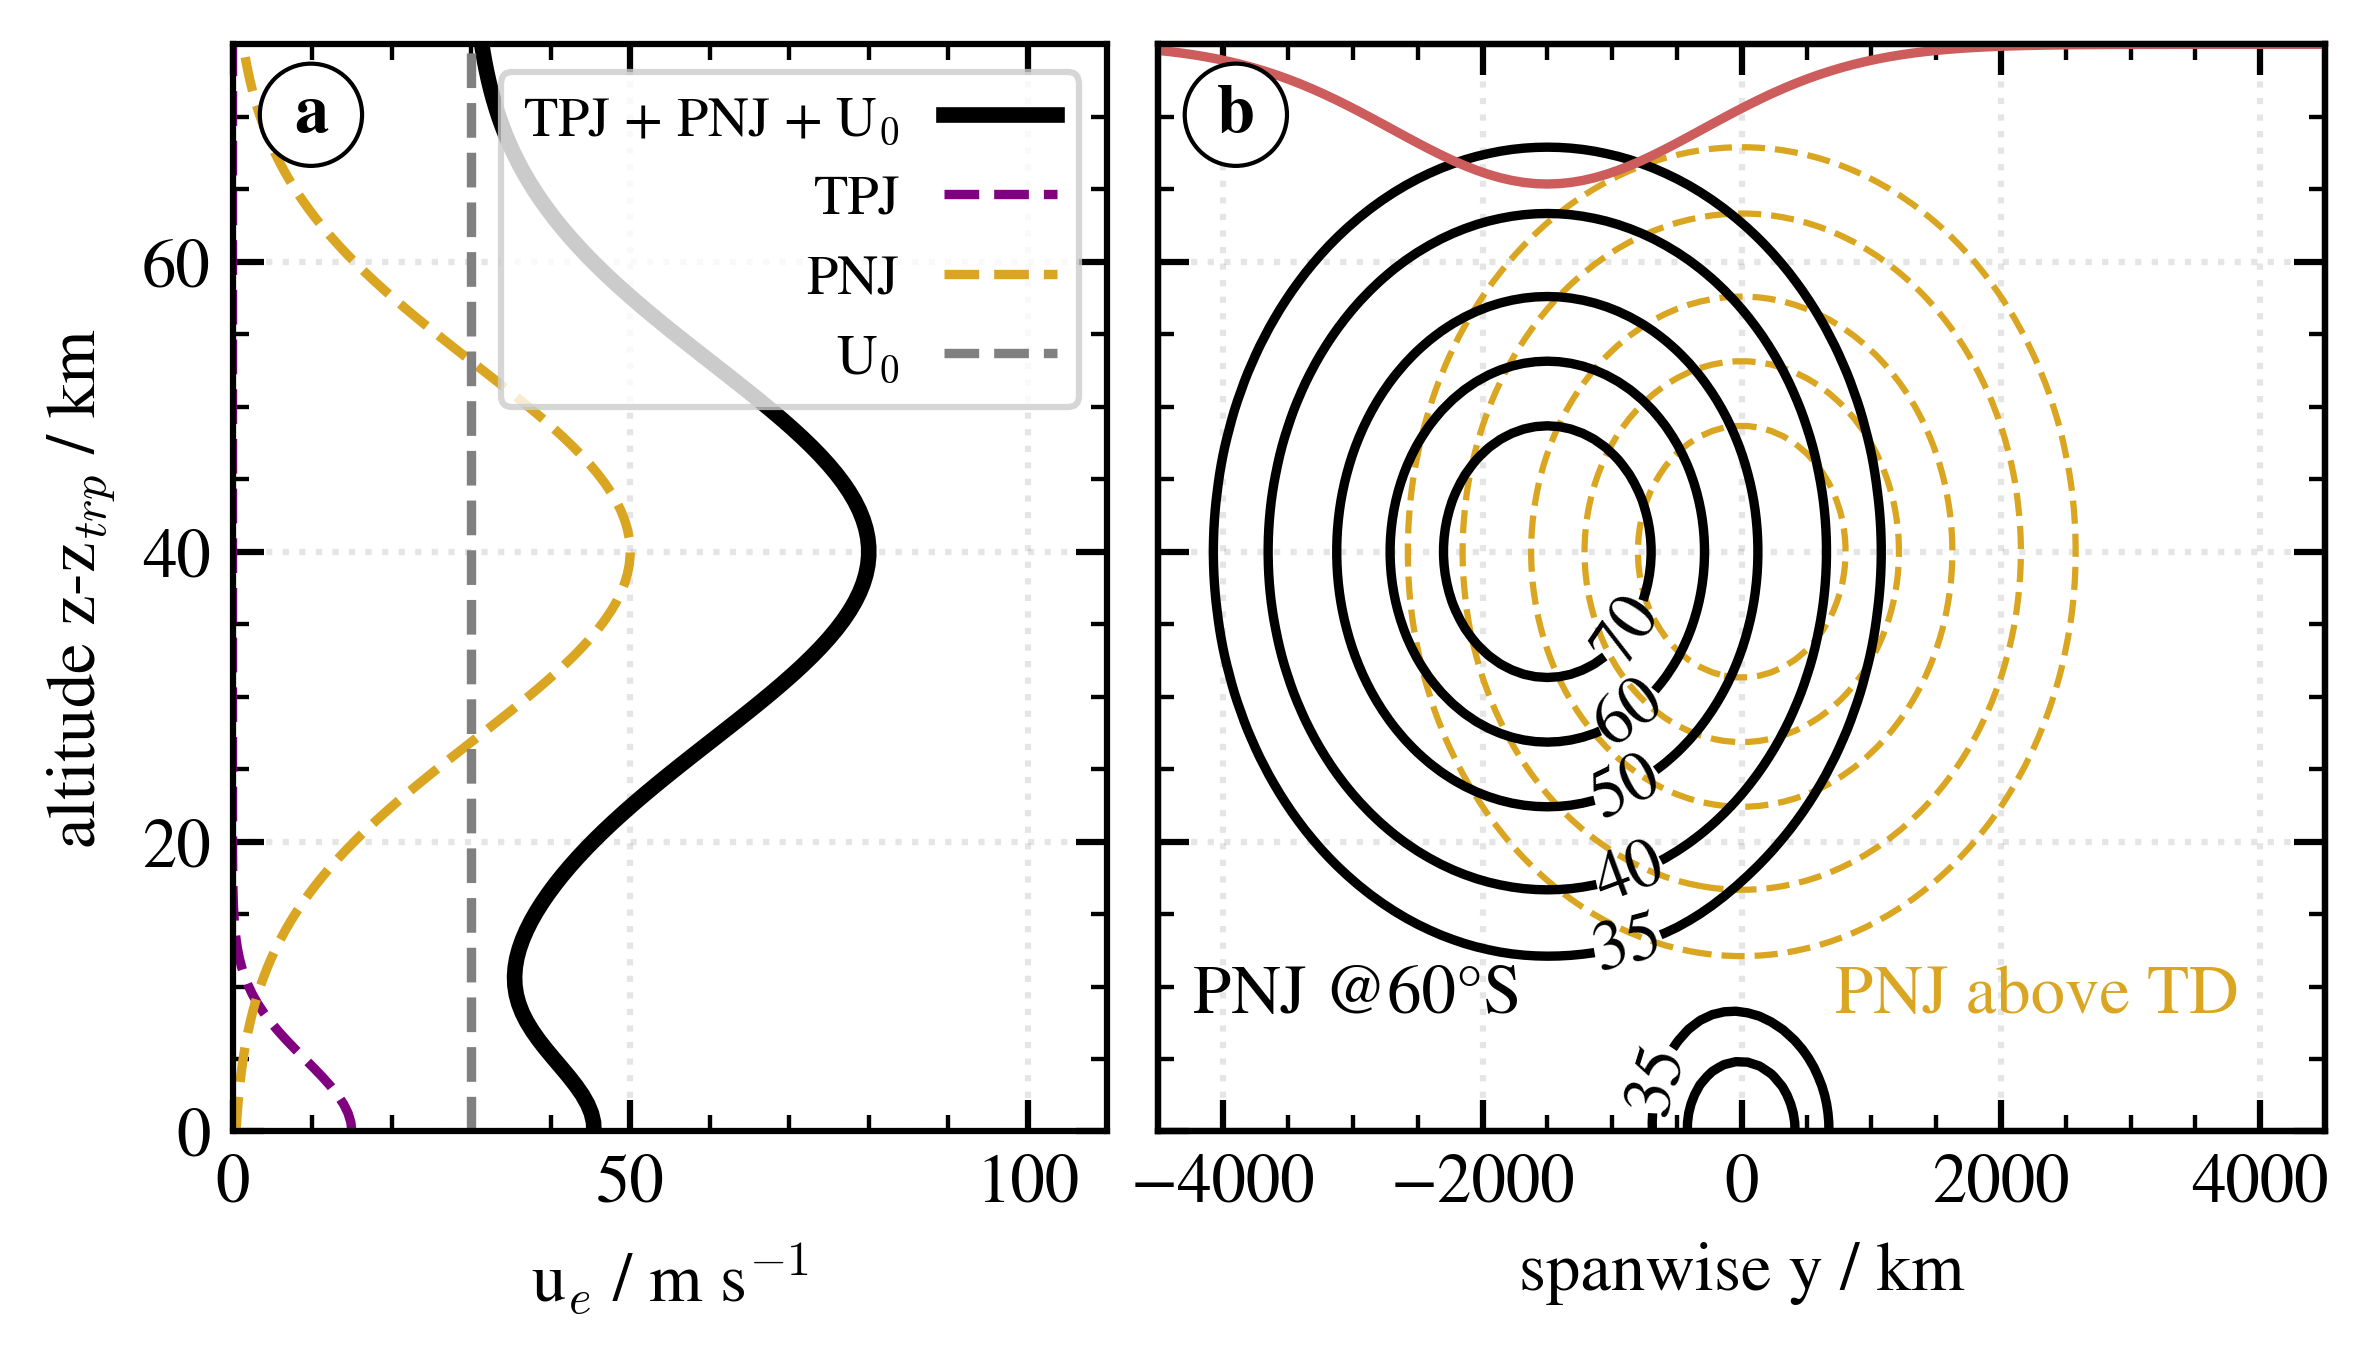
\includegraphics[width=0.75\textwidth]{figures_model/eulag-wind-profiles.png}
    \caption{Vertical profiles of the background wind for EULAG simulations with no meridional shear (a) and with meridional shear (b). The black line in (a) is a superposition of the tropopause jet TPJ (purple), the polar night jet PNJ (yellow) and a base wind U$_0$. Both jet distributions are based on equation (\ref{equ:wind-distribution}). The 2D wind profiles in (b) are obtained by combining the vertical profiles from (a) with a similar distribution in meridional direction (red curve in (b) for the PNJ at 60°S).}
    \label{fig:wind_profs}
\end{figure*} 
%
The meridional position of the PNJ varies during a winter season, but time averages show that it is mostly centered around a latitude of \SI{60}{\degree S} and south of the main stormtrack at tropopause level. To investigate the influence of the PNJ's merdional shear in chapter \ref{sec:results3D}, vertical profiles of $u_e(z)$ are multiplied with a meridional distribution (red line in Figure \ref{fig:wind_profs}b) to obtain variations of $u_e(z,y)$ visualized in Figure \ref{fig:wind_profs}b. The meridional distribution is set up in the same manner as equation \ref{equ:wind-distribution} with a $y_{jet}=\SI{1500}{\kilo\meter}$ and a standard deviation $\sigma_{jet}=\SI{1200}{\kilo\meter}$.

In EULAG idealized wind profiles are implemented within a new subroutine \code{tinit\_idealwind}\footnote[1]{The grey background refers to the name and implementation in the EULAG code.}. 

%%%%%%%%%%%% Transient boundary %%%%%%%%%%%%%%%%
\section{Transient lower boundary of idealized simulations}
\label{sec:trans-boundary}
When solving the anelastic equations (\ref{equ:momEqu}-\ref{equ:continuityEqu}) EULAG allows a time-dependent lower and upper boundary (\cite[]{prusa_propagation_1996} and \cite[]{wedi_extending_2003}). We utilize this feature to bound the numerical simulations at the tropopause and mimic a propagating tropopause fold at the lower boundary. This approach is not new and has already been used by \textcite[]{pfister_gravity_1993} or \textcite[]{prusa_all-scale_2003} to investigate NOGWs above a moving source. \\
The shape of a tropopause fold or, to be more specific, the shape of an isentrope above the tropopause that dips above the fold and rises again (compare with Figure \ref{fig:skerlakFold}) can be approximated by an upside-down isolated mountain.
The Witch of Agnesi
\begin{equation}
    h_{Agnesi}(x) = h_m \frac{L^2}{x^2+L^2}
    \label{equ:agnesi}
\end{equation}
is an established shape to describe isolated mountains in idealized simulations with the crest height $h_m$ and half width $L$. It was already used by \textcite{queney_problem_1948} to derive linear analytic solutions to a range of MW scenarios. Though non-linear simulations with a Witch of Agnesi are compared to Queney's solution in the next section to validate the model, the Witch of Agnesi is not appropriate to simulate a moving obstacle at the lower boundary. The topography following equation \ref{equ:agnesi} is non-zero for the whole domain of a discrete simulation (compare in Figure \ref{fig:topo_trans}). Therefore, the Witch of Agnesi would lead to a constantly changing surface at the domain's horizontal borders and impact the boundary conditions. This makes it a less appropriate shape for a moving topography or transient boundary in simulations. \\
A suitable alternative is a $1+cos(\frac{\pi}{4L}x)$ shape. It drops to 0 for $|\frac{x}{4L}| = 1$, so the sorrounding topography can be set to 0 for $|\frac{x}{4L}| \leq 1$ without sacrificing its continuity and differentiability. This is essential for the implementation of a transient boundary in the model. \textcite[]{prusa_all-scale_2003} already used a variation of the cosine function to mimic a moving tropopause fold in simplified 2D simulations with EULAG, but it exists a variation of the cosine function 
\begin{equation}
    h_{cos}(x) = 
    \begin{cases}
        & \frac{h_m}{16} (1+cos(\frac{\pi}{4L}x))^4, |\frac{x}{4L}| < 1 \\
        & 0, |\frac{x}{4L}| \geq 1 \\
      \end{cases}
    \label{equ:cosMtn}
\end{equation}
with a quite comparable shape to the Witch of Agnesi (equation (\ref{equ:agnesi})). Figure \ref{fig:topo_trans} shows how the shapes compare for a similar half-width and crest height and demonstrates that equation (\ref{equ:cosMtn}) is closest to the Witch of Agnesi. As long as the cosine mountain or depression is not too close to the edges the topography does not interfere with horizontal boundary conditions and all contributions to the surface pressure drag are now confined to a small neighbourhood around the peak. The cosine version of equation (\ref{equ:cosMtn}) has already been used for prescribing idealized topographies in 2D, too (\cite[]{epifanio_three-dimensional_2001} and \cite[]{metz_are_2021}). \textcite{metz_are_2021} state that the linear pressure drag across the cosine mountain of equation (\ref{equ:cosMtn}) is a factor of 1.3 higher compared to a corresponding Witch of Agnesi for a constant $N$ and $U$ environment.
\begin{figure*}[t]
    \centering
    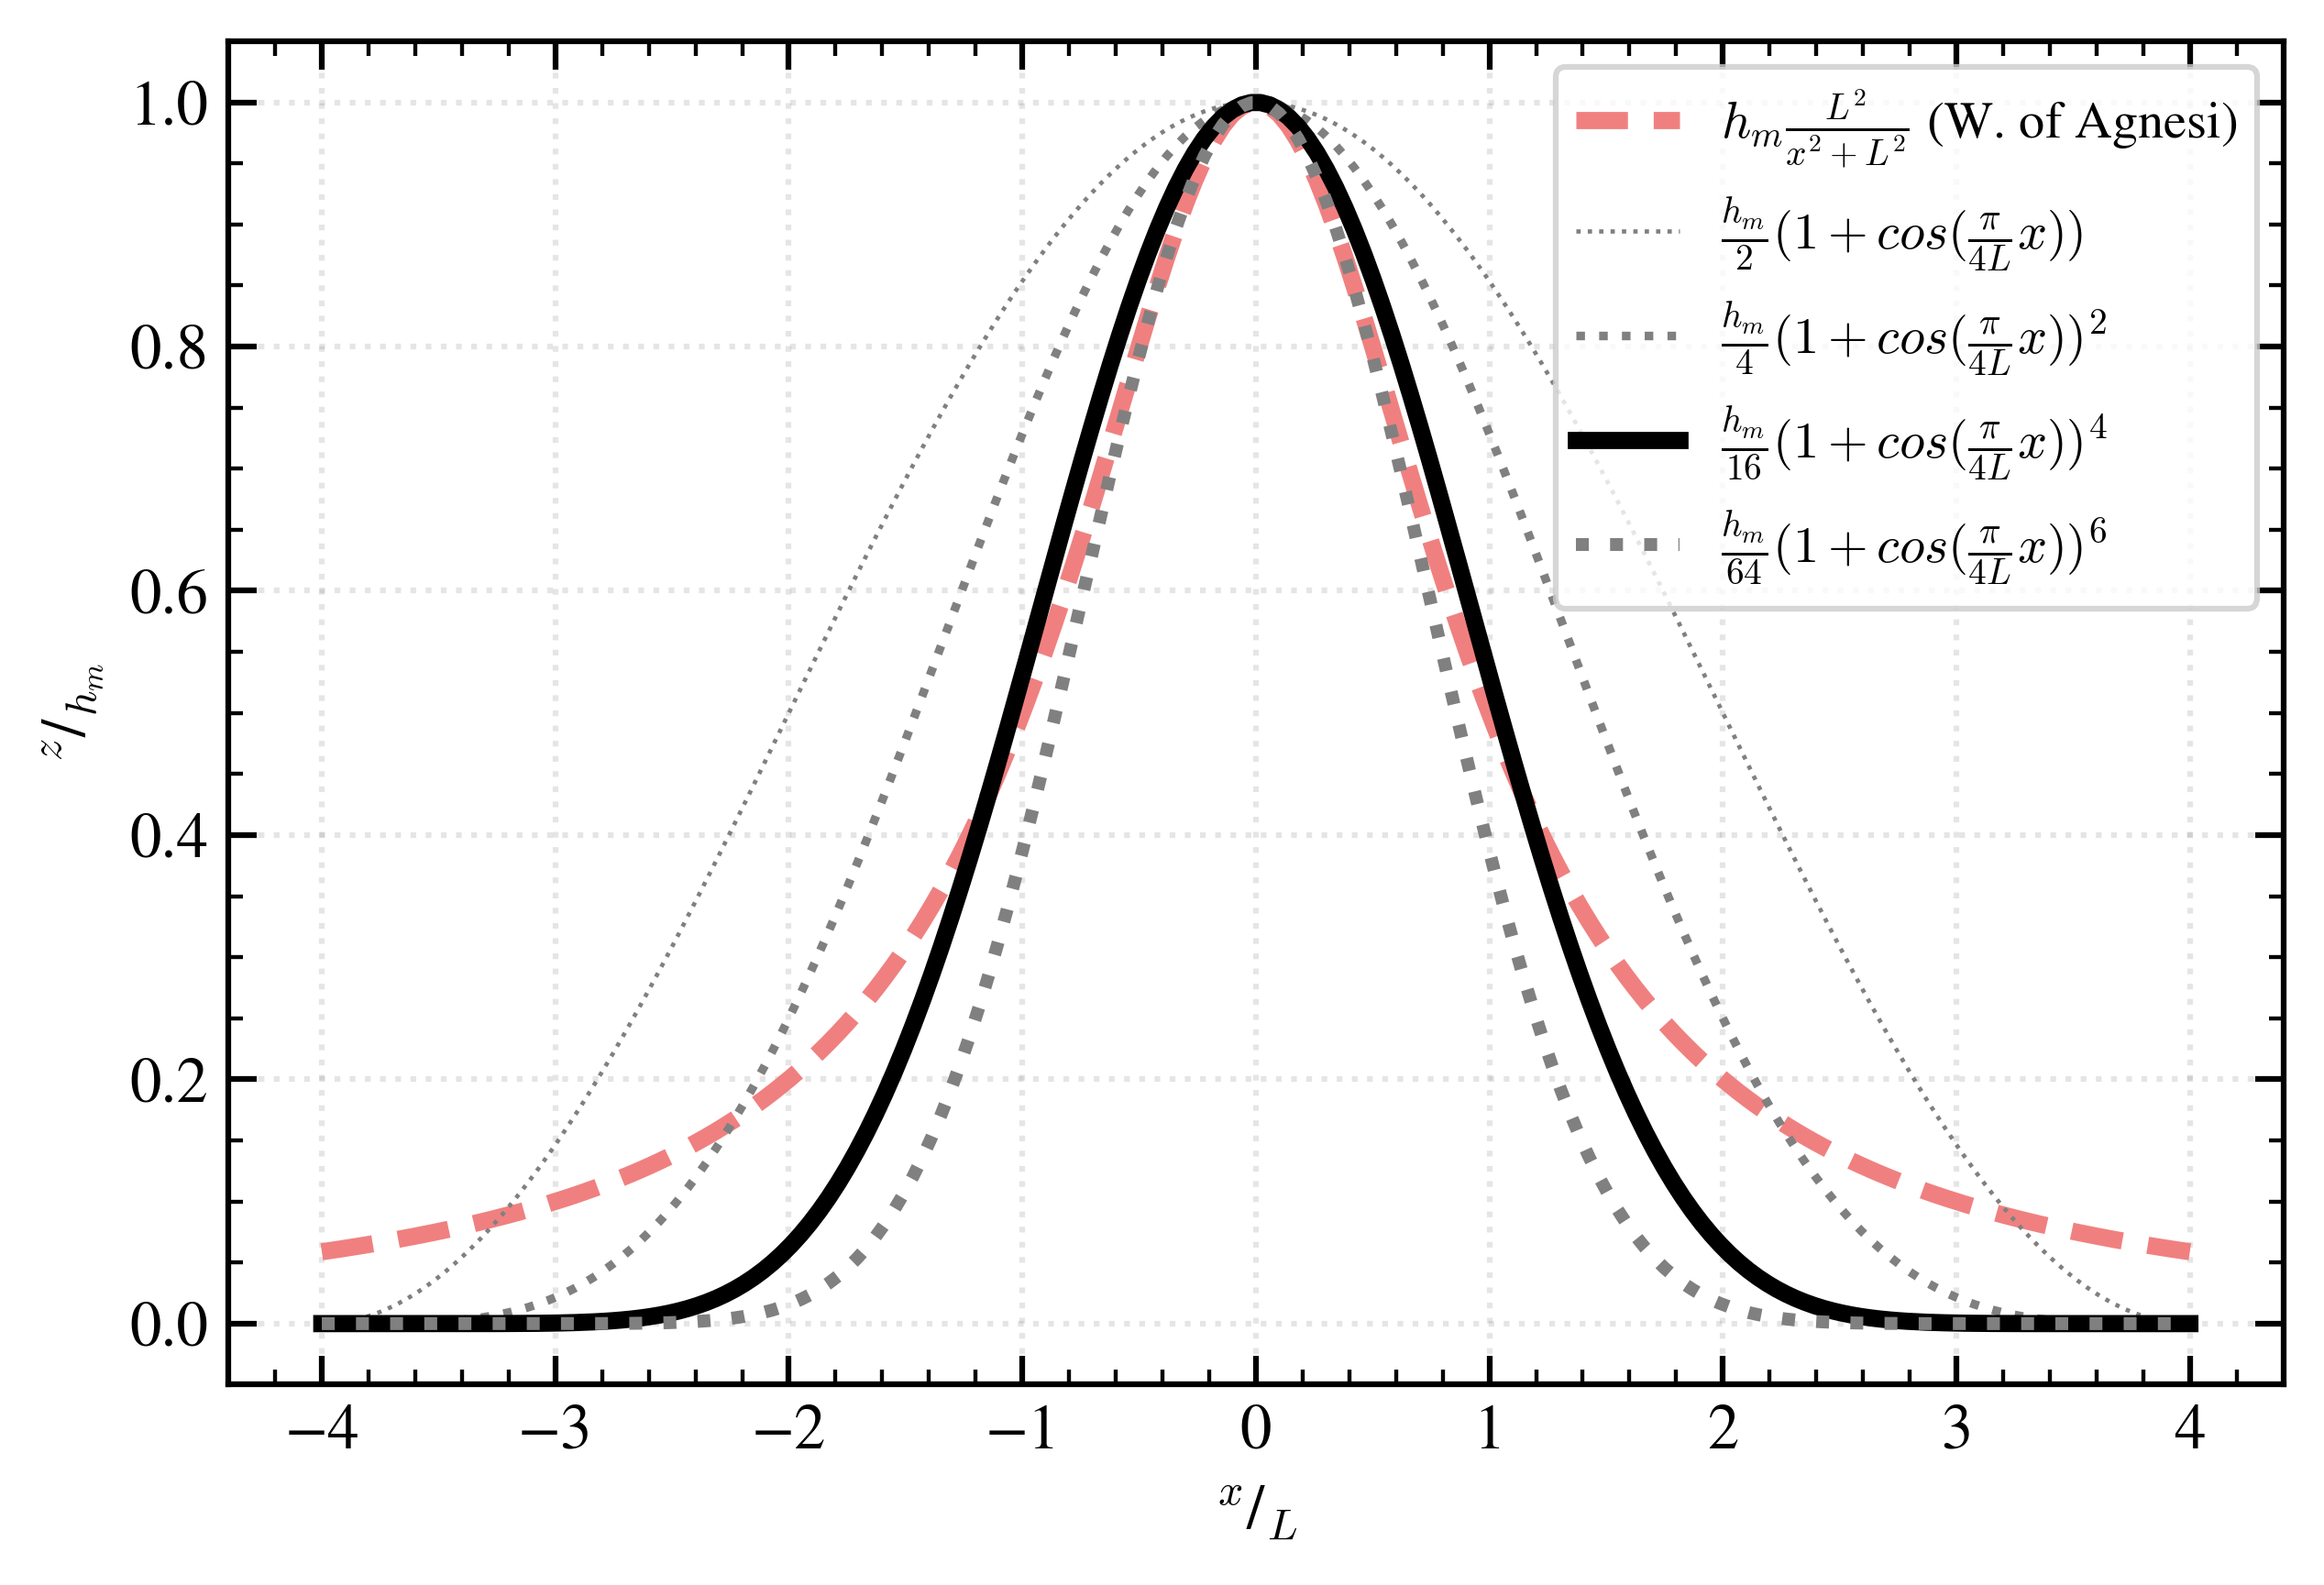
\includegraphics[width=0.67\textwidth]{figures_model/topo-transient-boundary.png}
    \caption{Shown are different variations of a $(1+cos(x))$ mountain (black solid and dotted lines) and a Witch of Agnesi (red dashed line). The vertical dimension is scaled by the mountain height $h_m$, the horizontal dimension by the mountain half width $L$. It allows a comparison of all shapes independent of $h_m$ and $L$.}
    \label{fig:topo_trans}
\end{figure*} 

In EULAG the transient surface boundary \code{zs} is defined within the subroutine \code{topol\_vert()}. \code{zs} and its time derivative \code{zsd} have to be continuous, so \code{zs} has to be differentiable. The following set of equations describe the time-dependent 2D surface \code{zs(tt,y,x)} for a 3D simulation of chapter \ref{sec:results3D} with an elliptical tropopause depression. Derivatives are left out and it should be noted that the equations vary for the elongated ridge (compare Figure \ref{fig:q3D_referenceSim}) in chapter \ref{sec:resultsQ3D}.
\begin{equation}
    \code{zs(tt,y,x)} = h_{cos}(\code{rr}) =\frac{1}{16} \bigl(1+cos(\frac{\pi}{4} \code{rr})\bigr)^4
    \label{equ:cosMtn-1}
\end{equation}
\begin{equation}
    \code{rr} = \sqrt{\bigl(\frac{\code{xx}}{\code{xml}}\bigr)^2 + \bigl(\frac{\code{yy}}{\code{yml}}\bigr)^2}
    \label{equ:cosMtn-2}
\end{equation}
\begin{equation}
    \begin{aligned}
        \code{xx} &= \code{cang}(\code{x}-\code{x0}) + \code{sang}(\code{y}-\code{y0}) \\
        \code{yy} &=-\code{sang}(\code{x}-\code{x0}) + \code{cang}(\code{y}-\code{y0}) 
    \end{aligned}
    \label{equ:cosMtn-3}
\end{equation}
\begin{equation}
    \begin{aligned}
    \code{x0} &= \code{x00} + \code{ctopo} \cdot \code{tt} \\ 
    \code{y0} &= \code{y00} = 0
    \label{equ:cosMtn-4}
    \end{aligned}
\end{equation}
with \code{xml} and \code{yml} being the width of the tropopause fold in zonal and meridional direction, \code{cang}=cos(\code{ang}) and \code{sang}=sin(\code{ang}) with \code{ang} being the angle of the fold's axes with respect to the domain axes. \code{ang} is used for rotating the tropopause fold in chapter \ref{sec:results3D}. \code{x00} and \code{y00} refer to the initial location of the fold's center and $\code{ctopo}=c_{tf}=\SI{13.88}{\meter \per \second}$ defines the propagation speed of the fold.

Another usecase of a time-dependent boundary or surface of the simulation is the initialization process. Idealized simulations with a surface topography start with a flat surface and homogeneous horizontal flow instead of initialising the flow field with a potential flow. Then the topography slowly grows for a defined time \code{tspinup}. In EULAG the surface \code{zs} is multiplied by
\begin{equation}
    \code{tf}(t) = t^3 (10 - 15t + 6t^2)
    % \code{tf}(\frac{\code{tt}}{\code{tspinup}}) = \Bigl(\frac{\code{tt}}{\code{tspinup}}\Bigr)^3 \biggl(10 - 15 \frac{\code{tt}}{\code{tspinup}} + 6 \Bigl(\frac{\code{tt}}{\code{tspinup}}\Bigr)^2\biggr)
    \label{equ:spin-up}
\end{equation}
with $t = \code{tt} / \code{tspinup}$ for $\code{tt} < \code{tspinup}$. The time derivative \code{zsd} is modified accordingly. \\
We use equation \ref{equ:spin-up} with $\code{tspinup}=\SI{12}{\hour}$ for a growing tropopause fold in all simulations. A wind ramping that slowly increases the surface wind to its stationary value can be an alternative strategy to circumvent unphysical processes during the initialization (e.g. \cite[]{mixa_nonlinear_2021}), but it is not used in the presented simulations.
% $c_{tf}$=\SI{13.88}{\meter \per \second} 

\section{Non-linear simulations of MW regimes with linear analytic solutions}
\label{sec:linear-MWs}
Though EULAG has proven itself to be a reliable tool for simulating a wide range of flows and specifically atmospheric flows over steep terrain (\cite{prusa_eulag_2008} and \cite{doyle_intercomparison_2011}) this section validates our specific model setup for simulating propagating tropopause folds. In a first step, we conducted simulations of a 'moving' mountain in a quiescent fluid (no background wind) and compared the propagation of GWs to our predictions from linear theory. In addition, we reproduced the 2D simulations of \textcite[]{prusa_all-scale_2003} with an oscillating tropopause fold at the lower boundary to confirm a correct implementation of the time-dependent boundary. We do not show these results and refer to the work of \textcite{grogger_simulation_2022} for further interesting experiments and tests with the EULAG model in general and specifically for transient boundary conditions. We focus instead on the comparison of non-linear model results from EULAG to analytic solutions of linear GW theory. 

The assumption of an impermeable tropopause at the lower boundary of the numerical simulations makes a tropopause depression act like an upside down mountain (valley) on the stratospheric flow above. In that sense, it is the goal to reproduce some fundamental analytic results of different MW regimes (non-hydrostatic GWs, hydrostatic GWs, inertia-gravity waves (IGWs)) with the EULAG model. \textcite{queney_problem_1948} was the first to derive linear solutions of the flow field for these different regimes assuming only small adiabatic perturbations. Many studies followed and contributed to a collection of analytic solutions for a wide range of scenarios. For the simplified cases of \textcite{queney_problem_1948} with a Witch of Agnesi mountain, constant background flow $U$ and stratification $N$ even solutions for the total gravity wave drag (GWD) exist, which can also be computed in numerical simulations (\cite[]{teixeira_physics_2014}). This makes the GWD a useful parameter to validate a numerical model with an analytic reference. Solutions are available for the whole range of mountain half widths $L$ and a concise summary on this topic is found in section 8.8 and Figure 8.10 in \textcite{gill_atmosphere-ocean_1982}. We will reproduce and discuss Figure 8.10 from \textcite[]{gill_atmosphere-ocean_1982} together with our model results and more recent theoretical studies in the next subsection. Subsequently, we continue with an interpretation of simulation based vertical profiles of momentum and energy fluxes, because they nicely illustrate various aspects in the context of momentum and energy conservation and the Eliassen-Palm (EP) relation. But first, we outline the numerical simulations of different MW regimes.

All simulations prescribe a Witch of Agnesi topography (equation (\ref{equ:agnesi})) with a small amplitude $h_m = \SI{100}{\meter}$ to minimize non-linear effects. Nine different mountain half widths from $L = 1-\SI{150}{\kilo\meter}$ are considered to cover the whole range of MW scenarios from non-hydrostatic GWs (high frequency waves) and hydrostatic GWs (medium frequency waves) to IGWs (low frequency waves). Ambient profiles follow the isothermal Bacmeister-Schoeberl model from section \ref{sec:ambient-profiles} with parameters for the troposphere (first column of table \ref{tab:ambientProfiles}). Therefore, $N=\SI{0.01}{\per\second}$ and the Coriolis frequency $f = 0.01 N = \SI{1e-4}{\per\second}$ (refers to a latitude of $\approx \SI{45}{\degree}$) and $u_e =\SI{10}{\meter\per\second}$ to be consistent with the analytic solutions in \textcite[]{queney_problem_1948} and \textcite[]{gill_atmosphere-ocean_1982}. \\
The horizontal domain and resolution varies between simulations, while the vertical dimension (z$_{top}=\SI{35}{\kilo\meter}$) and resolution ($\Delta$z$=\SI{50}{\meter}$) is fixed. The temporal resolution decreases for larger $L$ to reach a stationary state with the same amount of timesteps. All simulations simulate $n_t$=\SI{5760}{timesteps} on a grid with (n$_z$,n$_y$,n$_x$)=(701,48,960) grid points. Different resolutions are summarized in table \ref{tab:linearRegimes} which also provides relevant settings for vertical and horizontal sponge layers. These also change between simulations to ensure a smooth dissipation of wave energy and minimize wave reflection. \\
%
\begin{table*}[t]
    \centering
    \caption{Parameters for numerical simulations of different MW regimes: mountain width $L$, spatial increments $\Delta$x, $\Delta$y and $\Delta$z in the horizontal and vertical directions, time step $\Delta$t and the corresponding Courant-Friedrichs-Lewy (CFL) condition, thickness $\delta$x$_{ab}$ and time scale $\tau_x$ of the horizontal and altitude z$_{ab}$ and time scale $\tau_z$ of the vertical absorbers.}
    \begin{tabular}{@{}cccccccccc@{}}
    \toprule
    $L$/km & $\Delta$x/m & $\Delta$y/m & $\Delta$z/m & $\Delta$t/s & CFL/- & $\delta$x$_{ab}$/km & $\tau_x$/s  & z$_{ab}$/km & $\tau_z$/s \\ \midrule[1pt]
    1   & 50 & 2000 & 50 & 5 & 1 & 15  & 300  & 24 & 300   \\
    2   & 100 & 2000 & 50 & 5 & 0.5  & 30  & 600  & 24 & 450   \\
    5   & 250 & 5000 & 50 & 10 & 0.4 & 75  & 1200 & 24 & 600  \\
    10  & 500 & 10000 & 50 & 20 & 0.4  & 100 & 1800 & 24 & 900  \\
    25  & 1000 & 50000 & 50 & 40 & 0.4  & 200 & 3600 & 24 & 2400  \\
    50  & 1500 & 50000 & 50 & 60 & 0.4  & 300 & 4500 & 24 & 5400  \\
    75  & 2000 & 100000 & 50 & 60 & 0.3 & 400 & 6000 & 24 & 10500 \\
    100 & 2500 & 100000 & 50 & 75 & 0.3  & 500 & 7500 & 24 & 12000 \\
    150 & 3500 & 100000 & 50 & 180 & 0.51 & 700 & 9000 & 24 & 21000 \\
    \bottomrule
    \end{tabular}
    \label{tab:linearRegimes}
\end{table*}
The simulation for $L=\SI{100}{\kilo\meter}$ is shown in Figure \ref{fig:MWs-reference} with a vertical (a) and a horizontal (b) cross section after t$=\SI{120}{\hour}$. As expected for this large mountain width, IGWs propagate upward and into the lee of the mountain where they dissipate due to the sponge layers. Linear sponge or absorber layers are chosen quite thick to allow larger dissipation timescales $\tau$. Since $\Tilde{\alpha}$ and $\Tilde{\beta}$ in equations (\ref{equ:momEqu}) and (\ref{equ:potTemp}) of the anelastic framework are inverse proportional to $\tau$ (equation (\ref{equ:linear-sponge})) larger timescales $\tau$ reduce local forcings related to the damping and minimize wave reflection at the sponge interfaces and the model top. The meridional extent is very large to minimize any impacts of the ridge ends on the zonal cross section at y$=\SI{0}{\kilo\meter}$ that is used for the following analysis (calculating the total GWD and zonal averages of vertical profiles).
\begin{figure*}[t]
    \centering
    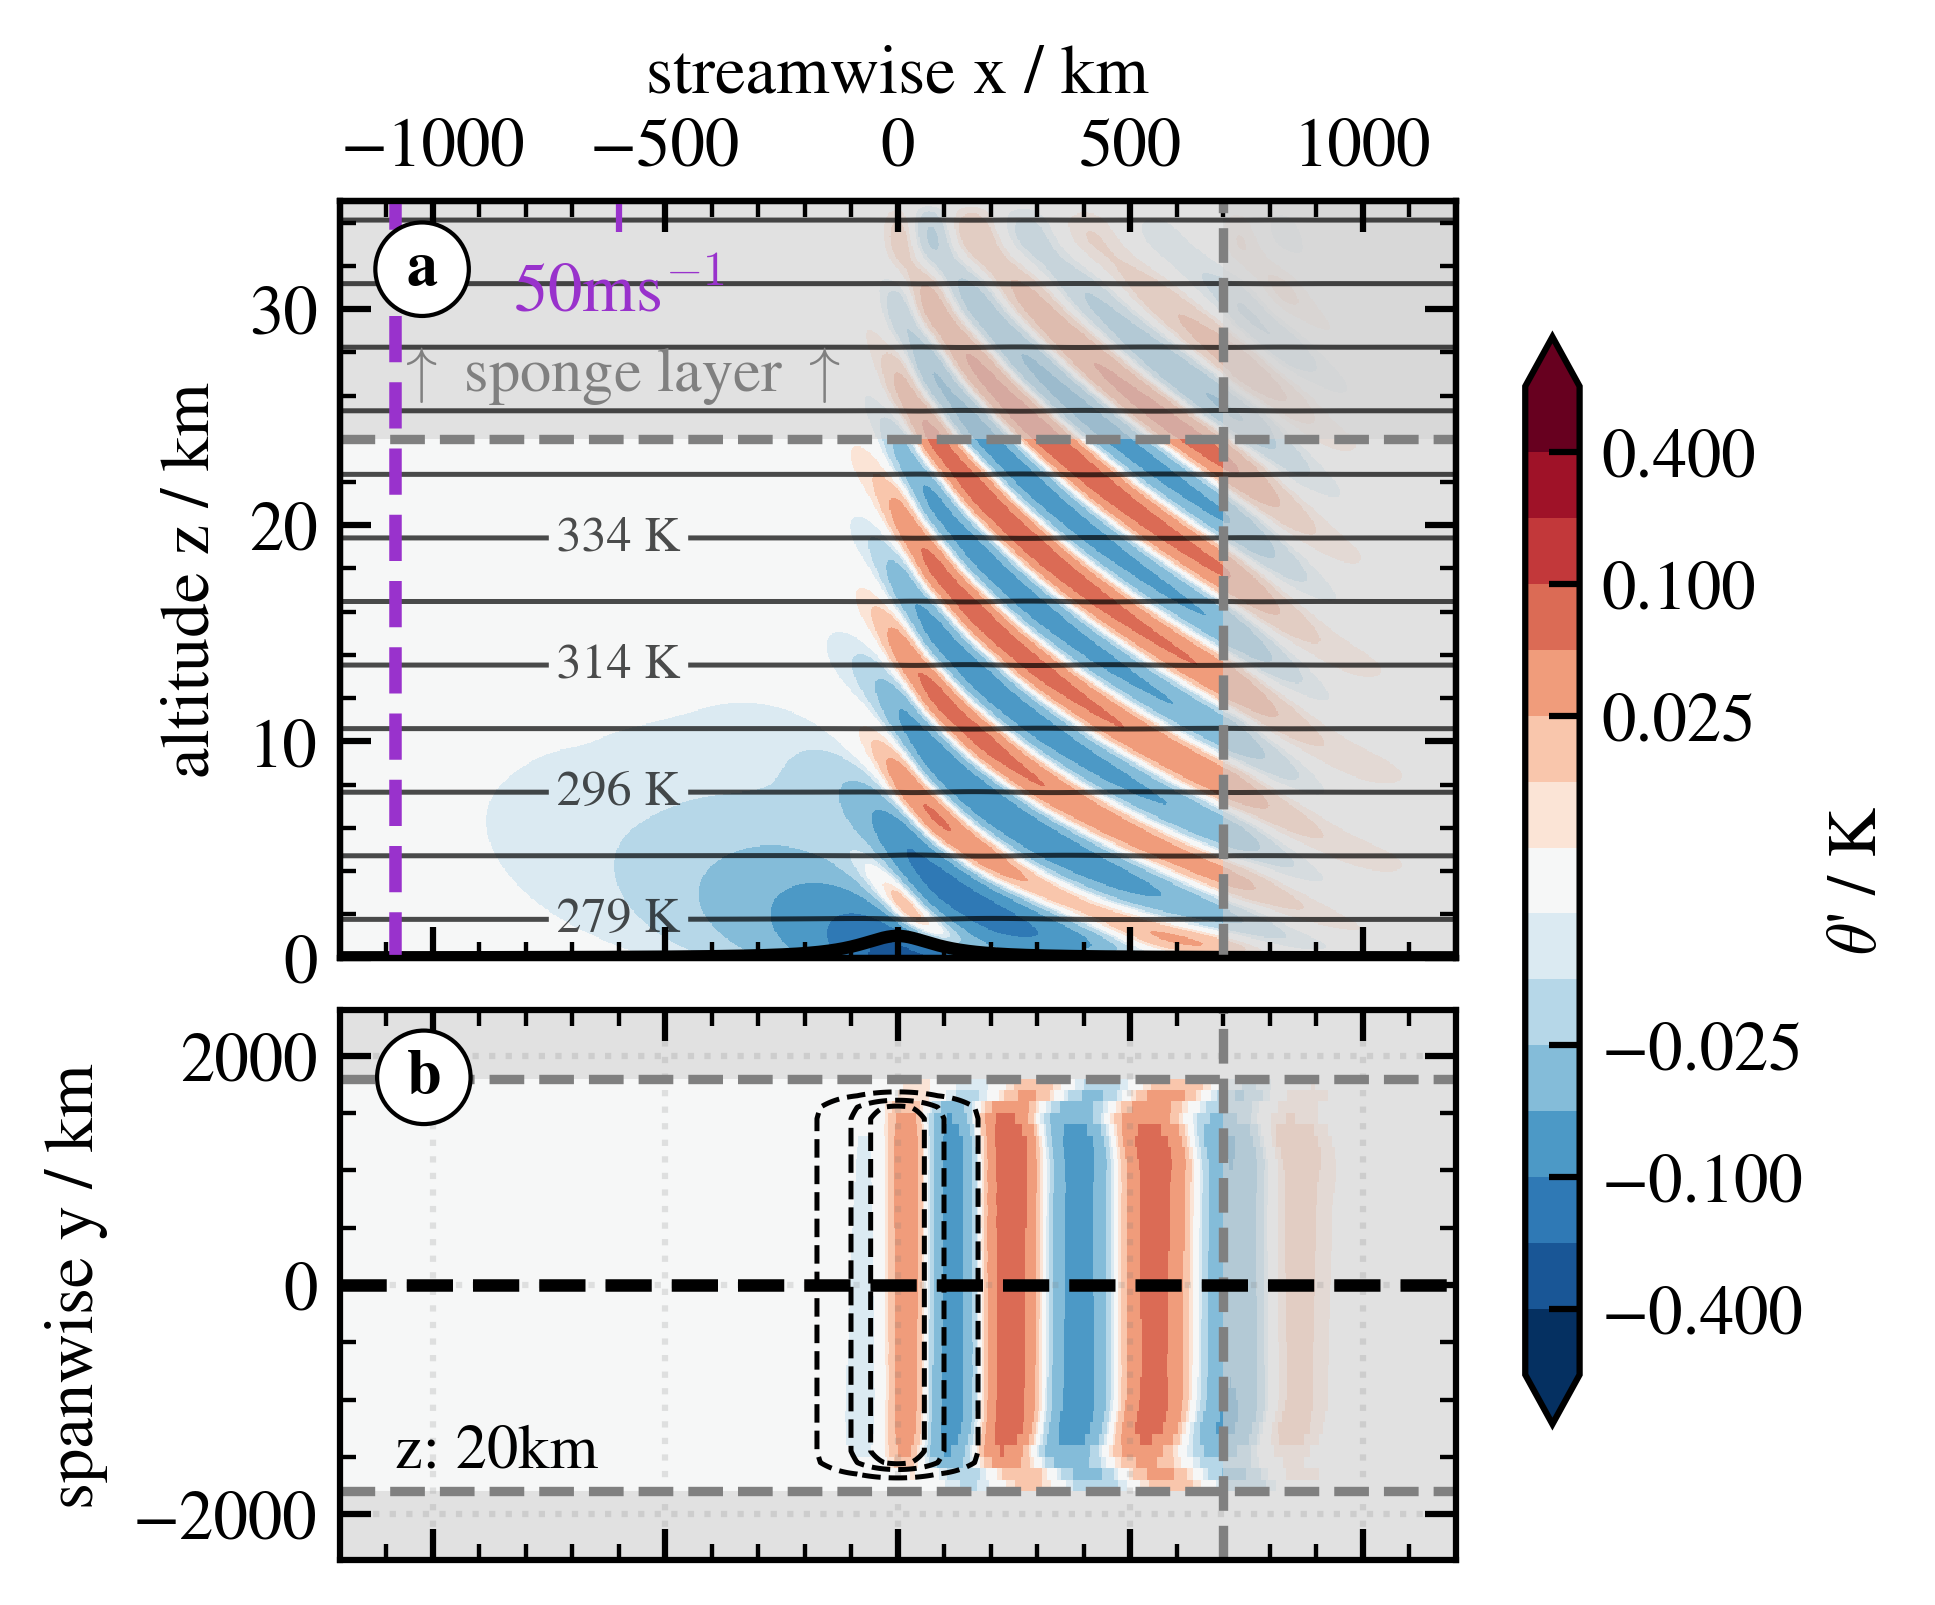
\includegraphics[width=0.67\textwidth]{figures_model/MWs-th-referenceSim.png}
    \caption{Centered vertical cross section (a) and horizontal cross section at z$=\SI{20}{\kilo\meter}$ (b) of potential temperature perturbations $\Theta'$ for a mountain width $L=\SI{100}{\kilo\meter}$ after t$=\SI{120}{\hour}$. Grey areas represent sponge layers (upstream sponge layer not shown) and the purple dashed line in (a) shows the constant wind profile with U$=\SI{10}{\meter\per\second}$. The thick dashed black line in (b) marks the relevant cross section for further analysis. The surface topography is exaggered by a factor of 10 and it should be noted that axes of (b) are not to scale.}
    \label{fig:MWs-reference}
\end{figure*}

% .􏰝α and β􏰝 are zero everywhere, except in the vicinity of the vertical and lateral boundaries where they increase linearly to one towards the model boundaries.
% courant number fulfilled?? 
% Wentzel-Kramers-Brillouin WHB method or approximation
% To be concise
%%%%%%%%%%%%%%%% GWD %%%%%%%%%%%%%%%%%
\subsection*{Gravity wave drag and angular momentum flux}
MW scenarios imply that an asymmetry in the pressure distribution across the mountain develops. Consequently, the atmosphere exerts a force on the orography that tends to accelerate the topography in the direction of the mean flow. This force  
\begin{equation}
    F_{GWD} = F_x = \int_{-\infty}^{\infty} p' \frac{\partial h}{\partial x} dx
    \label{equ:gwd}
\end{equation}
is called pressure drag and in the case of GWs it is also called gravity wave drag (GWD) (e.g. \cite[]{gill_atmosphere-ocean_1982} or \cite[]{durran_lee_2003}). Theoretical linear solutions for the GWD as a function of the mountain width exist for the whole spectrum of MWs assuming a steady state and only small adiabatic perturbations. While \textcite[]{blumen_momentum_1965} derived a solution for the high frequency spectrum (non-hydrostatic GWs), \textcite[]{smith_influence_1979} presented one for low frequency waves (IGWs). Both are based on Bessel functions and have been combined in Figure 8.10 of \textcite[]{gill_atmosphere-ocean_1982} to present a non-dimensional solution for the GWD for the whole range of mountain widths. Figure \ref{fig:GWD-MWs} also shows these solutions superimposed by results from our non-linear numerical simulations with the EULAG model and a more recent analytic solution from linear theory for the hydrostatic rotating limit. This alternative solution from \textcite{miranda_non-linear_1992} represented by the orange line in Figure \ref{fig:GWD-MWs} suggests a higher GWD for large mountain widths. Apparently, values from our non-linear simulations align with their results and not with the solution of \textcite[]{smith_influence_1979}. Is this plausible? \\
Smith's solution follows Queney's and assumes a steady flow that is independent of the y coordinate for the linearized Boussinesq equations of a rotating stratified fluid. In this case, independent of the y coordinate implies an infinite ridge shape and no pressure gradient in meridional direction in the momentum equation ($\frac{\partial p}{\partial y}=0$). The approach of \textcite[]{miranda_non-linear_1992} also uses the linearized Boussinesq equations for a rotating stratified fluid, but it allows $\frac{\partial p}{\partial y}\neq 0$ and keeps the 3D shape of a circular bell-shaped mountain as introduced by \textcite[]{smith_linear_1980} and \textcite[]{phillips_analytical_1984}. Instead, they assume zero meridional wind ($V=0$), integrate over two dimensions and end up with 
\begin{equation}
    F_{GWD} = \int_{-\infty}^{\infty} \int_{-\infty}^{\infty} p' \nabla h \, dx \, dy = \frac{\pi}{4} \rho_0 N U L h_0^2 \Bigl( \bigl(1 + \frac{2fL}{U}\bigr) e^{-\frac{2fL}{U}} \Bigr)
    \label{equ:gwd-miranda}
\end{equation}
for the hydrostatic rotating limit of a circular bell-shaped mountain. Though they define a circular mountain, the combination with $V=0$ seems to form a framework for linear solutions that match the numerical simulations with an elongated ridge. GWD values that result from non-linear simulations of a circular mountain are significantly lower.
 \begin{figure*}[t]
    \centering
    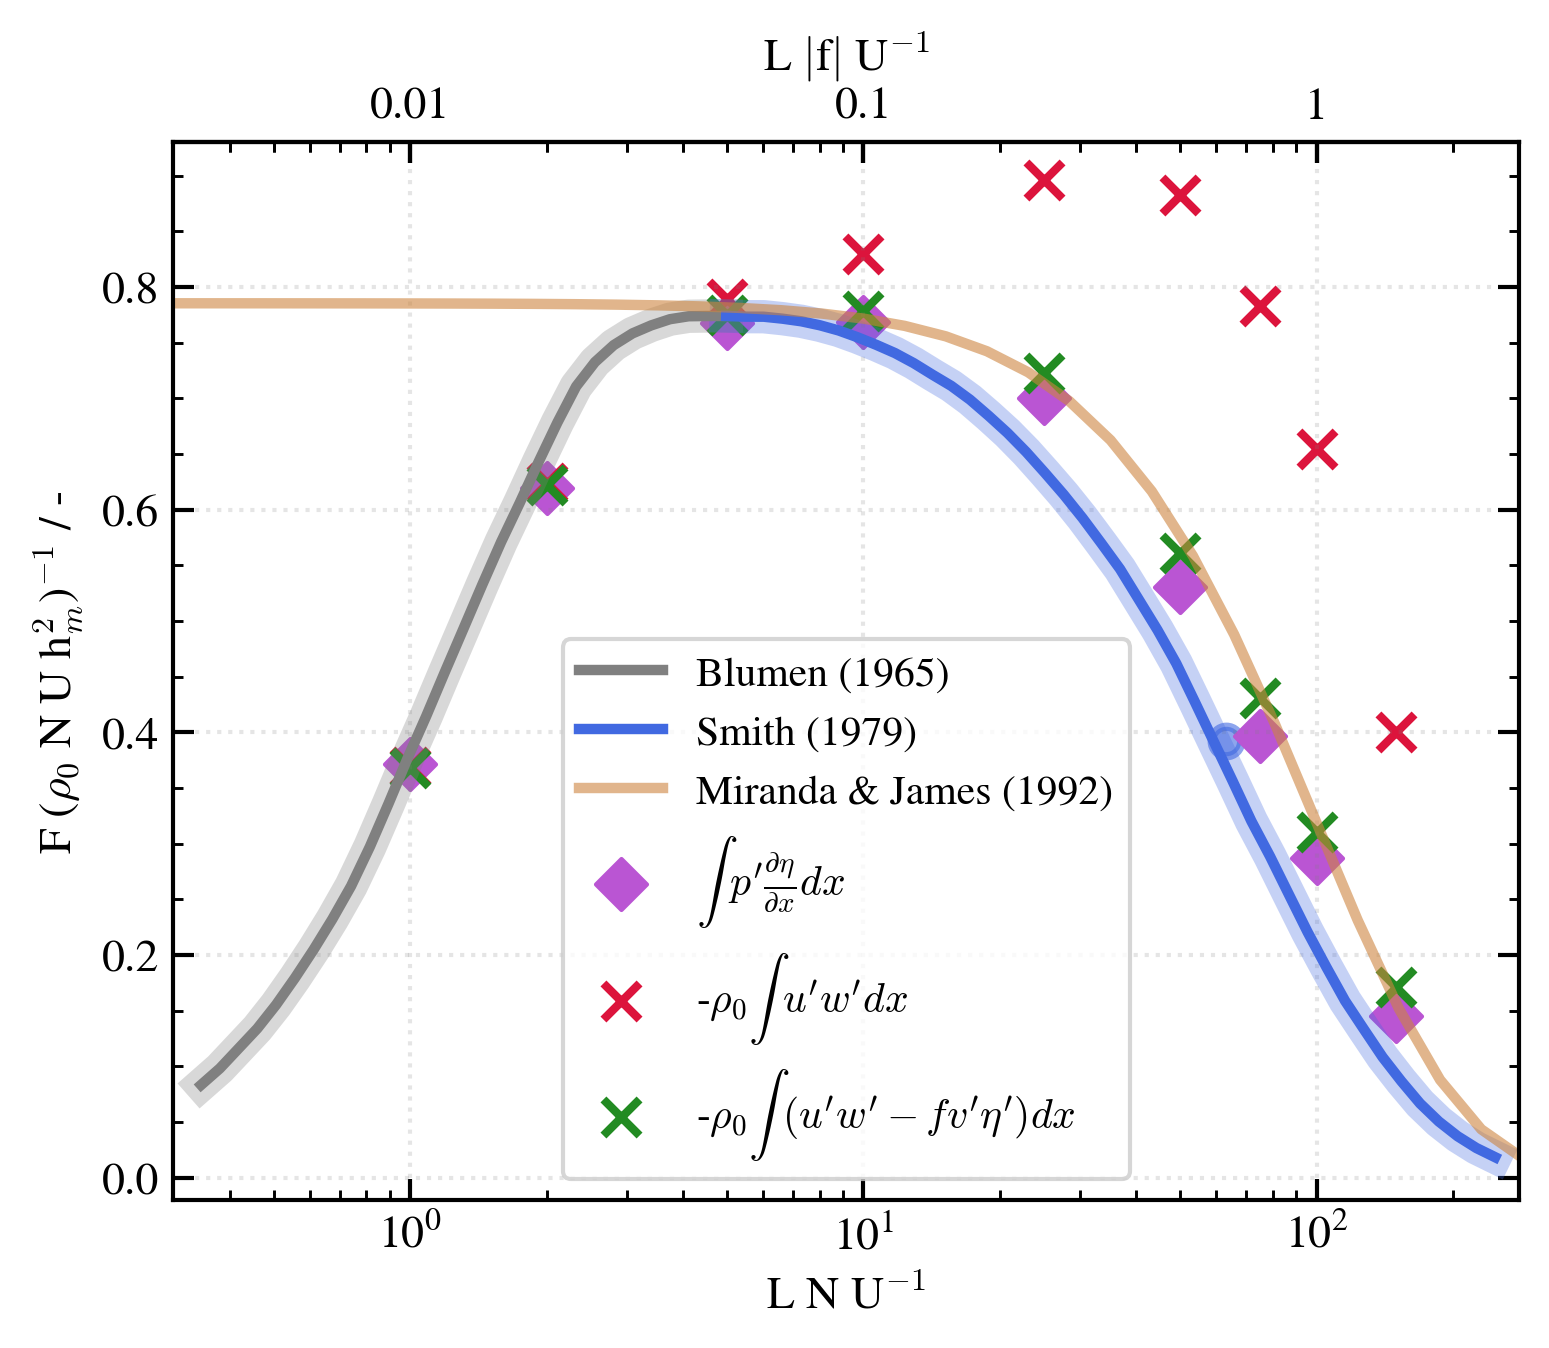
\includegraphics[width=0.63\textwidth]{figures_model/GWD-linearTheory-Q3D.png}
    \caption{The force $F$ is the GWD $F_x$ normalized by $\rho_0 \textrm{N} \textrm{U} \textrm{h}_m^2$ for the linear momentum flux of the flow over a Witch of Agnesi with half width $L$. Thicker faded lines indicate that the linear solution is based on Bessel functions (\cite[]{blumen_momentum_1965} and \cite[]{smith_influence_1979}). \textcite[]{miranda_non-linear_1992} provide an analytical solution for the hydrostatic rotating limit (IGWs). Buoyancy frequency N and flow speed U are uniform and the Coriolis frequency $f=0.01$N. Purple hashes represent the GWD or pressure drag, red crosses the linear momentum flux MF$_x$ and green crosses the angular momentum flux MF$_{x,ang}$ as described in \textcite[]{bretherton_momentum_1969}, \textcite[]{smith_influence_1979} and \textcite[]{broad_linear_1995} for different MW simulations with varying mountain half width $L$.}
    \label{fig:GWD-MWs}
\end{figure*}

Different values from the numerical simulations are plotted to emphasize the effect of rotation on the GWD. For a non-rotating fluid the vertical flux of horizontal momentum (for turbulent motion also called the Reynolds stress)
\begin{equation}
    (\mathrm{MF}_x, \mathrm{MF}_y) = \bar{\rho}  (\overbar{u'w'},\overbar{v'w'})
    \label{equ:mf}
\end{equation}
with the overbar denoting an average over one or multiple full wave cycles can be related to the GWD. Modifying the zonal momentum equation with the continuity equation, integrating throughout the volume from the surface $h(x)$ to an arbitrary height $z_t$ and considering that there is no advective momentum flux through the lower boundary yields
\begin{equation}
    \frac{\partial}{\partial t}\int_{}^{} \int_{}^{} \int_{}^{} \rho u' dV = - \left.\int_{}^{} \int_{}^{} \rho u'w' \, dx \, dy \right\vert_{z=z_t}  \,
    - \left.\int_{}^{} \int_{}^{} p' \frac{\partial h}{\partial x} \, dx \, dy \right\vert_{z=h}
    \label{equ:gwd-mf}
\end{equation}
and for a steady-state flow
\begin{equation}
    \left.\int_{}^{} \int_{}^{} p' \frac{\partial h}{\partial x} \, dx \, dy \right\vert_{z=h} =  -\left.\int_{}^{}  \int_{}^{} \rho u'w' \, dx \, dy \right\vert_{z=z_t}
    \label{equ:gwd-mf-2}
\end{equation}
the pressure drag equals the negative momentum flux (e.g. \cite[]{durran_lee_2003}). In other words, a positive pressure drag is compensated by a negative (downward) flux of horizontal momentum. \\
The negative zonal momentum flux MF$_x$ from equation (\ref{equ:mf}) is represented by the red crosses in Figure \ref{fig:GWD-MWs}. For smaller mountain widths up to $L=\SI{5}{\kilo\meter}$ it is more or less identical to the pressure drag (purple hashes), but starts to deviate as soon as rotational effects become important. \textcite[]{bretherton_momentum_1969} nicely illustrated why equation (\ref{equ:gwd-mf-2}) is not valid anymore for rotating fluids though MF$_x$ is still the momentum transfer across a flat horizontal surface (z$=$const.). He starts from the linearized momentum equation for a rotating fluid in the Boussinesq approximation
\begin{equation}
    U \frac{\partial u'}{\partial x} + w' \frac{\partial U}{\partial z} - f v' = -\frac{1}{\rho} \frac{\partial p'}{\partial x}
    \label{equ:momEqu-rotating}
\end{equation}
and notes that the pressure drag (equation (\ref{equ:gwd})) can be rewritten for the horizontal force across the wavy (not horizontal) surface z$= \eta(x)=h(x)$ to
\begin{equation}
    F_x =  \int_{-\inf}^{\inf} p' \frac{\partial \eta}{\partial x} dx = -\int_{-\inf}^{\inf} \eta' \frac{\partial p'}{\partial x} dx
    \label{equ:pdrag-rotating}
\end{equation}
by applying integration by parts. We follow the notation of \textcite[]{smith_influence_1979} or \textcite{broad_linear_1995} and use $\eta$ for the vertical and not the meridional displacement. Equation (\ref{equ:momEqu-rotating}) becomes 
\begin{equation}
    F_x =  -\int_{}^{} \rho u' \Bigl(U \frac{\partial \eta}{\partial x}\Bigr) \, dx + \rho \frac{\partial U}{\partial z} \int_{}^{} w' \eta' \, dx  - f \int_{}^{} \rho v' \eta' \, dx 
    \label{equ:momEqu-rotating-2}
\end{equation}
and after linearizing with $w'=U\frac{\partial \eta}{\partial x}$ the second term vanishes and
\begin{equation}
    F_x = \mathrm{MF}_{x,ang} = -\int_{}^{} \rho u'w' \, dx  -  \int_{}^{} \rho f v' \eta' \, dx
    \label{equ:angular_momentum}
\end{equation}
with a first term representing the vertical flux of linear momentum MF$_x$ and a second term that represents the Coriolis force acting in the region between the undisturbed, leveled streamline and the vertically displaced streamline. For rotating fluids it is equation (\ref{equ:angular_momentum}) that is equal to the pressure drag of equation (\ref{equ:gwd}). It is called the vertical flux of angular momentum and can be interpreted as the force exerted across a surface always consisting of the same material particles (Lagrangian perspective) that differs from the linear momentum across a horizontal plane (Eulerian perspective) by the Coriolis term in equation (\ref{equ:angular_momentum}). \\
In Figure \ref{fig:GWD-MWs} the angular momentum is represented by the green crosses. It is slightly higher than the pressure drag for larger mountain widths, but the difference is small. It was checked if compressible effects can explain this difference considering the compressible solution of the GWD from linear theory 
\begin{equation}
    F_x =  \rho_0 \int_{}^{} (u'w' + f v' \eta') \, dx + f \int_{}^{} \rho' v' \eta' \, dx
    \label{equ:angular_momentum_compressible}
\end{equation}
derived by \textcite[]{broad_linear_1995}. Dropping the Boussinesq approximation adds another term to the streamwise GWD involving density fluctuations. However, the normalized contribution of the compressible part $f \rho' v' \eta'$ in equation (\ref{equ:angular_momentum_compressible}) was at maximum $\mathcal{O}(10^{-5})$ and can not explain the difference between the pressure drag and the angular momentum in Figure \ref{fig:GWD-MWs}. It is not fully understood what causes this inconsistency of the pressure drag, but theories exist and will be discussed in the context of vertical profiles in the next subsection. 

Overall, GWD values from non-linear simulations with EULAG successfully reproduce analytic solutions of the GWD from linear theory for the whole range of MWs from non-hydrostatic GWs to IGWs. In particular, the surface angular momentum MF$_{x,ang}$ closely follows the linear solution of \textcite[]{miranda_non-linear_1992} for the hydrostatic rotating limit.

% Though $V=0$, 3D critical layers might be relevant for the 3D flow of IGWs with increasing meridional perturbations $v'$ for larger mountain widths as discussed in section \ref{sec:q3D-wind}. but vertical profiles in next section suggest that all simulations obey linear wave propagation... from EP relation. 

% ecause in plane inertio-gravitational waves a vertical displacement 5 is correlated with a Ox displacement ( and hence with an Oy velocity v, these contributions are systematically of one

% \cite[]{jones_propagation_1967} was first before bretherton 
% \cite[]{teixeira_physics_2014}
% gaussian quadrature 
% dimensionless drag is specified differently for Smith and miranda due to additional dimension

% Geostrophic balance: fu = - 1/rho * dp/dy
% f negative for southern hemisphere but not for idealized simulations of MWs
% possible to run EULAG simulation with meridional gradient of p?
% Are results interesting for further investigation of ini probs? I guess this geostrophic balance develops but can we filter out its contribution to p'?

%%%%%%%%%%%%%%%% VERTICAL PROFILES %%%%%%%%%%%%%%%%%
\subsection*{Vertical profiles of momentum and energy fluxes}
For linear, non-rotating (2D), steady-state flows equation (\ref{equ:gwd-mf-2}) is valid for any upper level $z_t$, so the linear momentum is conserved in the vertical as long as U$\neq 0$ (\cite[]{durran_lee_2003}). In their seminal work \textcite[]{eliassen_transfer_1960} present a consistent result relating the linear momentum flux to the gradient of the vertical flux of wave energy EF$_z = \overbar{p'w'}$
\begin{equation}
    -\frac{\partial}{\partial z}\overbar{p'w'} = \frac{\partial U}{\partial z} \cdot \bar{\rho} \overbar{u'w'}
    \label{equ:EP-relation-dudz}
\end{equation}
and to EF$_z$ directly
\begin{equation}
    \begin{aligned}
    -\overbar{p'w'}& = U \cdot \overbar{u'w'} \\
    -\mathrm{EF}_z& = U \cdot \mathrm{MF}_x.
    \end{aligned}
    \label{equ:EP-relation}
\end{equation}
Equation (\ref{equ:EP-relation}) is called the Eliassen-Palm (EP) relation and is valid for linear, steady, small-amplitude, non-dissipative wave propagation. Under these assumptions, equation (\ref{equ:EP-relation-dudz}) and (\ref{equ:EP-relation}) again state that the vertical flux of horizontal momentum is conserved in the vertical and that EF$_z$ changes in proportion to the gradient of $U(z)$. For $U(z)=$const. EF$_z$ does not change with height, too.

\textcite[]{broad_linear_1995} combined the analysis methods of \textcite[]{eliassen_transfer_1960} and \textcite[]{bretherton_momentum_1969} to obtain a similar set of equations for the general case of a 3D rotating fluid. Modifying the 3D energy equation according to \textcite[]{eliassen_transfer_1960} provides 
\begin{equation}
    -\frac{\partial}{\partial z} \mathrm{EF}_z = \frac{\partial U}{\partial z} \cdot \mathrm{MF}_{x,ang} + \frac{\partial V}{\partial z} \cdot \mathrm{MF}_{y,ang}
    % U(z) \cdot \frac{d}{dz}\mathrm{MF}_{x,ang} + V(z) \cdot \frac{d}{dz}\mathrm{MF}_{y,ang} = 0
    \label{equ:EP-relation-rotating-dudz}
\end{equation}
and considering the horizontal momentum across the wave surface $z=\eta(x,y)$ (not the horizontal surface) according to \textcite[]{bretherton_momentum_1969} yields
\begin{equation}
    \begin{aligned}
        -\overbar{p'w'}& = U \cdot \bar{\rho_0} (\overbar{u'w'} + f \overbar{v' \eta'}) + V \cdot \bar{\rho_0} (\overbar{v'w'} - f \overbar{u' \eta'}) \\
        -\mathrm{EF}_z& = U \cdot \mathrm{MF}_{x,ang} + V \cdot \mathrm{MF}_{y,ang}
    \end{aligned}
    \label{equ:EP-relation-rotating}
\end{equation}
from the horizontal momentum equations. In a nutshell, MF$_x$ in the non-rotational case is replaced by the vertical flux of angular momentum MF$_{x,ang}$ and for a zonal background flow with $V=0$ conclusions are the same as above: MF$_{x,ang}$ is conserved in the vertical as long as $U(z) \neq 0$ and EF$_z$ changes proportional to the gradient of $U$.

\begin{figure*}[t]
    \centering
    \includegraphics[width=0.99\textwidth]{figures_model/Queney-MWs-zprofiles.pdf}
    \caption{Zonal averages of vertical profiles for the vertical fluxes of zonal momentum MF$_x$ and MF$_{x,ang}$ (a), vertical energy flux EF$_z$ (b), horizontal energy flux EF$_x$ (c) and the potential energy density $E_p$ (d) for a range of MW simulations with varying mountain half width $L$. (b) also shows vertical profiles of \textbf{MF}$\cdot$\textbf{U} and (e) shows the difference between \textbf{MF}$\cdot$\textbf{U} and -EF$_z$ scaled with the corresponding surface value to illustrate the validity of the Eliassen-Palm relation considering the linear momentum MF$_x$ (solid lines) and angular momentum (dashed lines). All profiles are filtered in the vertical with a cutoff wavelength $\lambda_{z,filter}=\SI{9}{\kilo\meter}$. Note the logarithmic scale of the x-axis in (a) and (b).}
    \label{fig:MWs-zprofiles}
    % Do this plot for 2,4,8,32,64,128,256
\end{figure*}

In the previous section, the vertical displacement of a streamline $\eta'$ was replaced by the topography $\eta'=h(x)$ for calculating surface values of MF$_{x,ang}$. To investigate vertical profiles of MF$_{x,ang}$ in the numerical simulations $\eta'$ can be approximated by $\Theta'$
\begin{equation}
    \Theta' \approx  \eta' \frac{\partial \bar{\Theta}}{\partial z}
    \label{equ:thprime}
\end{equation}
assuming an adiabatic flow along isentropes. Then equation \ref{equ:angular_momentum} becomes
\begin{equation}
    \mathrm{MF}_{x,ang} = \bar{\rho} (\overbar{u'w'} + f \overbar{v' \eta'}) = \bar{\rho} (\overbar{u'w'} + f \frac{1}{\frac{\partial \bar{\Theta}}{\partial z}}\overbar{v' \Theta'})
    \label{equ:angular_momentum_theta}
\end{equation}
and allows the direct calculation of MF$_{x,ang}$ on all model levels for (a), (b) and (e) in Figure \ref{fig:MWs-zprofiles}. \\ 
Overall, Figure \ref{fig:MWs-zprofiles} illustrates how vertical profiles of the momentum and energy fluxes change when increasing the mountain width L from a non-hydrostatic to a hydrostatic rotating wave regime. In (a) the linear and angular momentum are compared. As expected, vertical profiles of MF$_x$ and MF$_{x,ang}$ are identical for small mountain widths, but deviate for larger $L$ due to rotational effects. (a) also shows that MF$_x$ is conserved in the vertical for those simulations with negligible Coriolis effect, but decreases vertically in magnitude for $L \geq \SI{25}{\kilo\meter}$ (in agreement with conclusions for non-rotating case above). From equation (\ref{equ:EP-relation-rotating-dudz}) and (\ref{equ:EP-relation-rotating}) we would expect that MF$_{x,ang}$ is conserved for all simulations. Compared to MF$_x$ the vertical profile of MF$_{x,ang}$ is much closer to a constant value, but a decrease in lower layers of the atmosphere is still noticeable. Allocating this decrease to non-linear processes in the simulations is questionable, because the conservation of MF$_x$ and MF$_{x,ang}$ for small mountain widths up to $L=\SI{10}{\kilo\meter}$ is nearly perfect. In addition, dashed lines in (b) and (e) in the same figure illustrate that the EP-relation for a rotating fluid (equation (\ref{equ:EP-relation-rotating})) holds for all simulations suggesting a linear wave propagation and negligible non-linear effects. In this context, vertical profiles of EF$_z$ (dotted lines in (b)) have to show an identical pattern to MF$_{x,ang}$, because $U(z)=$const. and $V(z)=0$, so equation (\ref{equ:EP-relation-rotating}) directly relates MF$_{x,ang}$ and EF$_z$. It follows that we also observe decreasing values for EF$_z$ with height thought we would expect a constant profile for a constant background wind $U$. The original EP-relation (equation (\ref{equ:EP-relation})) for a non-rotating fluid is only fulfilled when rotational effects are negligible. For large mountain widths solid lines in (b) deviate from dashed lines and the relative difference between -EF$_z$ and \textbf{MF}$\cdot$\textbf{U} in (e) grows. \\
It is not clear, why vertical profiles of MF$_{x,ang}$ (and consequently EF$_z$) slightly decrease with height for large mountain widths. Most likely, this is related to the offset of the surface pressure drag for large $L$ in Figure \ref{fig:GWD-MWs} with respect to the angular momentum. Maybe the initialization of the problem is not fully consistent with the linear solutions when rotational effects become important. Overthinking the initialisation and ensuring a balanced geostrophic flow might be instructive, but other reasons can not be ruled ruled out. Tuning the diffusivity of the model or further reducing the mountain height $h_m$ to minimize the wave amplitudes could be alternative approaches.
% Mittelung auf Modellflächen als Erklärung??

To provide a comprehensive overview on momentum and energy fluxes vertical profiles of the zonal energy flux EF$_x = \overbar{u'p'}$, the potential energy 
\begin{equation}
    E_p = \frac{1}{2} \Bigl(\frac{g}{N}\Bigr)^2 \overbar{\Bigl(\frac{T'}{\bar{T}}\Bigr)^2}
    \label{equ:epot-density}
\end{equation}
and kinetic energy
\begin{equation}
    E_k = \frac{1}{2} \Bigl(\overbar{u'^2} + \overbar{v'^2} + \overbar{w'^2}\Bigr)
    \label{equ:ekin-density}
\end{equation}
with the total energy $E_0 = E_k + E_p$ (\cite[]{tsuda_global_2000}) are visualized in Figure \ref{fig:MWs-zprofiles}, too.\\
For $ \SI{25}{\kilo\meter} < L < \SI{75}{\kilo\meter}$ EF$_x$ transitions from being unexceptionally negative and decreasing in magnitude with height to a partially positive and also increasing EF$_x$ close to the surface (Figure \ref{fig:MWs-zprofiles}c). This transition towards a positive EF$_x$ at the surface for wider mountains is a consequence of the Coriolis force and even more pronounced for tropopause folds in Chapter \ref{sec:resultsQ3D} (compare for example to Figure \ref{fig:q3D_ctropo_vert} or \ref{fig:q3D_wind}). In addition, the meridional energy flux EF$_y$ increases close to the surface for larger mountain widths (dotted lines in (c)) because meridional perturbations $v'$ increase and are strongest at the surface. This deviation from a purely zonal flow could be the reason for the small inconsistencies in Figure \ref{fig:MWs-zprofiles} for the centered streamwise cross section, too.\\
(d) also shows a transition at the surface for $E_p$ and $E_k$ with a surface minimum for the hydrostatic regime with $L \approx 5-\SI{10}{\kilo\meter}$. For smaller and larger mountain widths both energies increase again at the surface, so zonal averages of $E_p$ and $E_k$ at the surface seem to be inversely proportional to the GWD which decreases for smaller and wider mountains (compare Figure \ref{fig:GWD-MWs}). At higher altitudes $E_p$ and $E_k$ clearly decrease for increasing mountain half widths $L$.\\ 
% Potentially, these findings are related to the vertical profiles of the angular momentum flux discussed above, but variations of EF$_x$, $E_p$ and $E_k$ due to rotational effects are much more pronounced and rather reflect realistic profiles for a streamwise cross section.
Another instructive observation in (d) comes from estimating the ratio $\frac{E_k}{E_p}$. It is close to 1 for high- to midfrequency waves, but the kinetic energy becomes more dominant for low frequency waves with significant Coriolis force (\cite[]{gill_atmosphere-ocean_1982}). The numerical simulations with EULAG indisputably reflect this relation with almost equivalent profiles of $E_k$ and $E_p$ for small mountain widths and a larger $E_k$ for large widths.

Though open questions on the vertical profiles of MF$_{x,ang}$ remain, Figure \ref{fig:MWs-zprofiles} provides a meaningful summary of momentum and energy fluxes for the whole range of MW regimes and illustrates which relations and assumptions are appropriate for individual simulations. In particular, valid EP-relations with the angular momentum (rotating fluid) for all MW scenarios in Figure \ref{fig:MWs-zprofiles}e imply a reliable setup of the EULAG model.

% what about langrangian view of flux calculation...??

% \cite*[]{jones_propagation_1967}

% with U and V  $\rho_0$ the background wind and density  notation of \textcite[]{broad_linear_1995}. 

% \cite[]{durran_lee_2003}
% Furthermore, a classic theorem due to Eliassen and Palm states that under the preceding assumptions ρ0u′w′ is constant with height except at a “critical level” at which u = 0.
% Mountain waves are dissipated at the mean-state critical layers found in real atmospheric flows. Mountain waves are also dissipated through breaking and overturning if they attain sufficiently large amplitude

% \cite*[]{broad_linear_1995}
% The drag force may be effectively zero and T constant in magnitude and direction only when the basic-state wind U(z) traverses back on itself across orographic wave numbers for which stress has already been removed lower down (remembering of course that the absorption at lower critical levels is never entirely total but dependent on the Richardson number
% Three-dimensional analysis shows that the generalization of the 2-D result is for all vertical levels to be potential critical levels dependent on the underlying orographic Fourier spectrum

% Pseudomomentum is conservative wave propagation -> how does it relate angular momentum? f=0 -> reynolds stress is conserved for non-rotational GWs as stated by EP.

% For rotational fluids the reynolds stress changes with changing winds / because pseudo momentum is consserved but intrinsic frequency changes. is angular momentum changing, too?

% Include thermal wind relation in simulations... representation of gradient in y direction due to 3D nature of IGWs
% Reynolds stress and the momentum flux in a non-rotational environment or under the mid-frequency approximation.

%%%%%%%%%%%%%%%% LESSONS LEARNED %%%%%%%%%%%%%%%%%
\subsection*{Lessons learned from non-linear simulations of MW cases}
It might be useful to recapitulate important parameters and settings of the idealized non-linear numerical simulations to replicate results like the GWD from linear theory:

\begin{itemize}
    \item In retrospect, it is undisputed that full 3D simulations with meridional gradients have to be conducted to correctly incorporate rotational (Coriolis) effects. Only for entirely 3D simulations and analytical approaches (\cite[]{miranda_non-linear_1992}) the solutions converge. This was not clear from the beginning. 
    \item Domain sizes should be large enough to minimize damping effects and reflection at the boundaries, but it has to be verified that horizontal and vertical resolutions are sufficient, too. In particular, the vertical resolution had to be high to obtain accurate perturbations at the surface and, ultimately, correct values for the pressure drag and surface momentum fluxes for the performed MW simulations. 
    \item A correct initialisation of the simulation can be very important and its effect might still be observed after long simulation times. It can be useful to introduce a wind ramping or a growing topography to circumvent unwanted effects.
    \item The choice of horizontal and vertical sponge layers and corresponding settings can have a large effect on the simulation due to wave damping within the sponge and reflection of waves at the sponge interface. If absolute values of perturbations are less important it can be useful to introduce an exponential sponge layer in the vertical dimension that continuously increases from the bottom to the top of the domain. In that case, the absorber is described by
    \begin{equation}
        \Tilde{\chi} = \frac{1}{\tau} e^{\frac{z-z_b}{\zeta_z}}
        \label{equ:exp-sponge}
    \end{equation}
    for an arbitrary relaxation factor $\Tilde{\chi}$ ($\Tilde{\alpha}$ or $\Tilde{\beta}$ in the anelastic equations) that is inversely proportional to a timescale $\tau$. $\zeta_z$ scales the vertical structure of the exponential absorber that starts at $z=0$ and $z_b$ is the domain boundary (top). An exponential sponge throughout the whole domain can simplify simulations, because it gets rid of interactions at a sponge interface. If, however, absolute values of e.g. a total GWD are important, the exponential absorber effects these values already at the first model level though damping close to the surface is very small. For such a purpose, a linear sponge that starts at a certain model level $z_{ab}$ and increases linearly towards the model boundary $z_b$ is the preferable option. In EULAG it is defined by
    \begin{equation}
        \Tilde{\chi} = 
        \begin{cases}
            & \frac{1}{\tau} \frac{z-z_{ab}}{z_{b}-z_{ab}}, z \geq z_{ab} \\
            & 0, z < z_{ab} \\
        \end{cases}
        \label{equ:linear-sponge}
    \end{equation}
    and its extent $z_{b}-z_{ab}$ and timescale ${\tau}$ have to be tuned carefully to minimize reflections at the sponge interface $z_{ab}$ and at the model boundary $z_b$.
\end{itemize}


\newpage
\thispagestyle{plain}

% ==== CHAPTER 4 ===============================================================
% ---- set some counters to zero:
\setcounter{equation}{0}
\setcounter{table}{0}
\setcounter{figure}{0}
% ---- include tex-file:
\chapter{NOGWs excited by tropopause depressions in a 2D plane}
\label{sec:resultsQ3D}
It is the goal of this chapter to address the second research question
\begin{tcolorbox}[]
    (R1) How sensitive are NOGWs from propagating tropopause depressions to the depression's 2D shape and to 2D properties of the stratospheric environment?
\end{tcolorbox}
\noindent and identify zonal and vertical properties of the tropopause and the stratospheric environment that significantly influence the appearance and propagation of NOGWs above propagating tropopause folds. \\
At first, section \ref{fig:q3D_referenceSim} presents the reference simulation for this sensitivity study and recapitulates important assumptions and properties of the simulations. Then three sections investigate variations of the GW activity in the stratosphere when changing the propagation speed of the tropopause fold (section \ref{sec:q3D-speed}), the zonal shape of the tropopause fold (section \ref{sec:q3D-shape}) and the vertical profile of the ambient wind or the Coriolis force (section \ref{sec:q3D-wind}). A short summary (section \ref{sec:q3D-summary}) completes this analysis. 

\section{The reference simulation}
\label{sec:resultsq3D-reference}
\begin{figure*}[t]
    \centering
    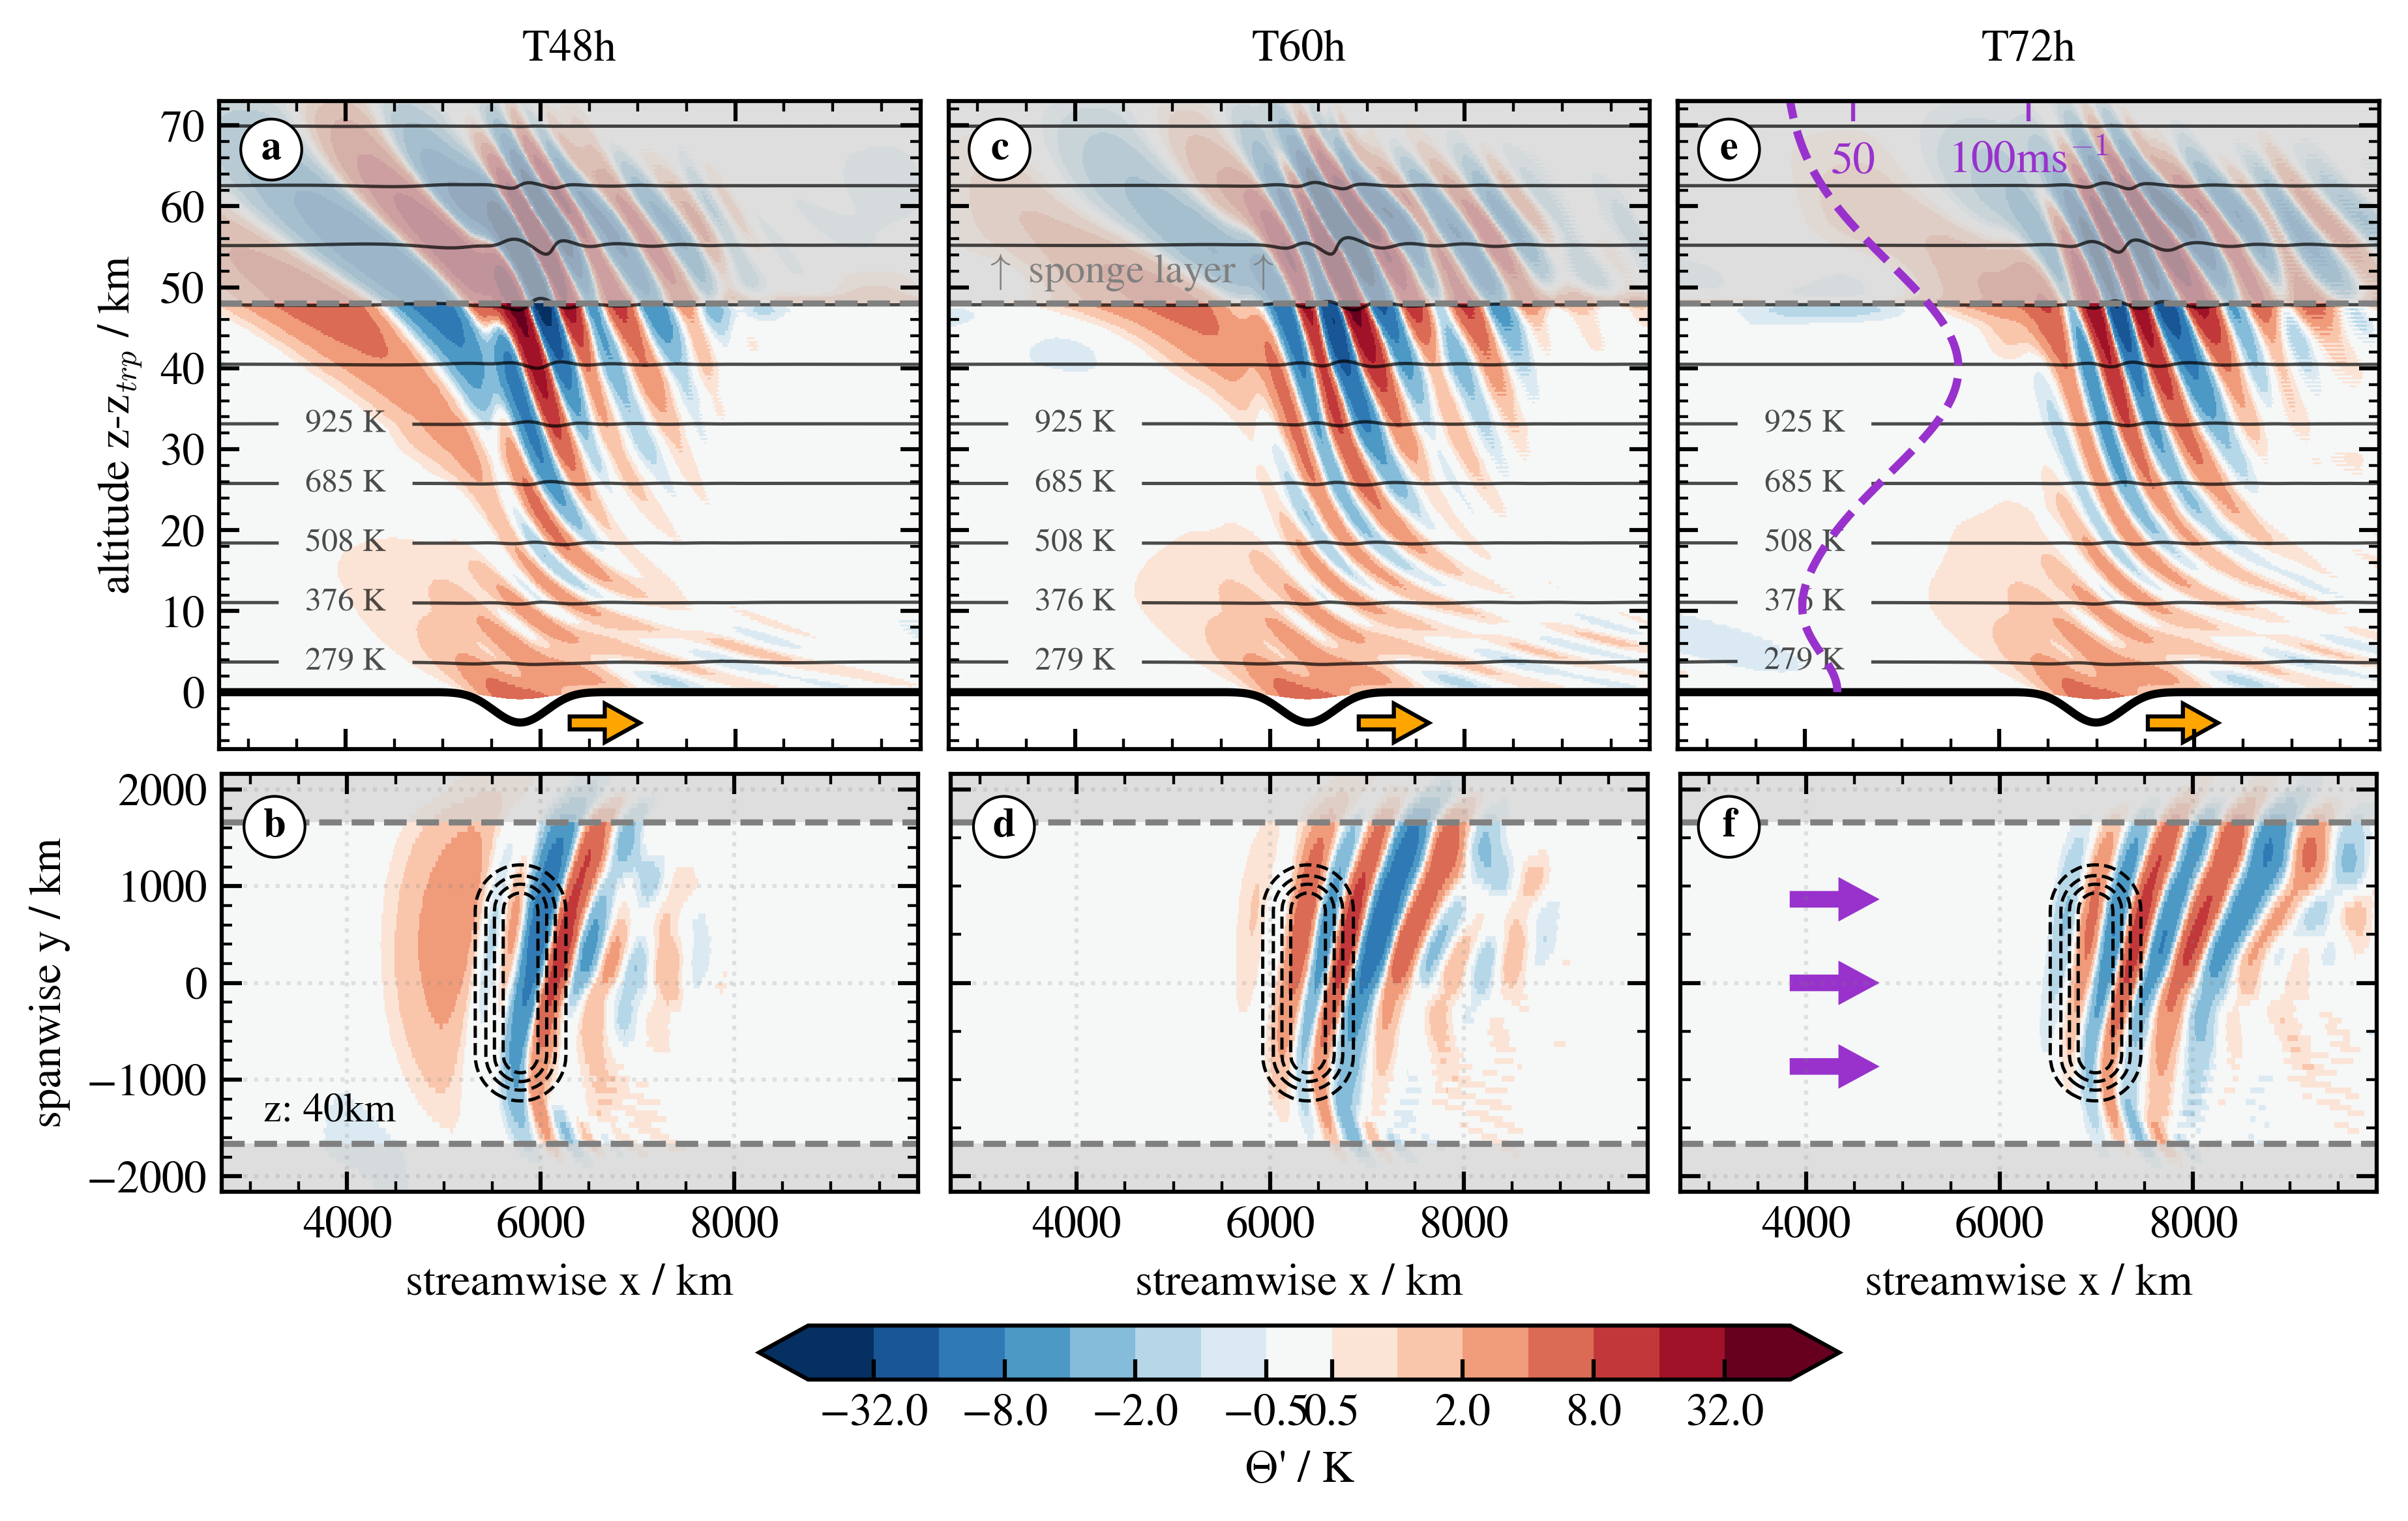
\includegraphics[width=0.99\textwidth]{figures_q3D/Q3D-th-referenceSim.png}
    \caption{Visualized is $\Theta'$ for three timesteps of the reference simulation in vertical cross sections (a), (c) and (e) for y=0 and horizontal cross sections (b), (d) and (f) \SI{40}{\kilo\meter} above the tropopause. The tropopause fold at the lower boundary moves with a constant speed $c_{tf}=\SI{13.88}{\meter\per\second}$ towards the right. Its height is exaggered by a factor of 5 and thin lines above represent constant potential temperature. The vertical ambient wind profile (purple line in (e)) is constant in meridional direction as indicated in (f). Dashed lines in the horizontal cross sections define the shape of the elongated fold and grey areas indicate sponge layers.}
    % of the sensitivity study
    \label{fig:q3D_referenceSim}
\end{figure*}
%
The model validation (section \ref{sec:linear-MWs}) showed that a correct integration of rotational (Coriolis) effects requires 3D simulations. Consequently, all simulations in this chapter are 3D though the following analysis focuses on the 2D plane at y=0. Figure \ref{fig:q3D_referenceSim} illustrates the reference simulation for the sensitivity study. As indicated in Figure \ref{fig:q3D_referenceSim}e and f, the background wind $u_e(z)$ only changes in the vertical direction and is constant in meridional direction. In a similar manner, the meridional shape of the lower boundary (dashed lines in horizonal cross sections) is constant in the center of the domain and only changes close to the sponge layers. The zonal shape of the transient boundary is prescribed by the cosine function (equation (\ref{equ:cosMtn})) and it propagates with a constant speed $c_{tf}=\SI{13.88}{\meter\per\second}$ in the direction of the arrows. To recap, the transient, impermeable and frictionless lower boundary mimics the tropopause or more precisely an isentrope just above the tropopause. This isentrope still dips above a tropopause fold, but it does not reach areas within the fold that are prone to increased mixing. For the reference simulation the half width of the fold is $L = \SI{300}{\kilo\meter}$ and the maximum depth of the fold is \SI{750}{\meter}. The ambient background atmosphere is isothermal (Bacmeister-Schoeberl Model described in section \ref{sec:ambient-profiles}) and follows the stratosphere setup from table \ref{tab:ambientProfiles} with a constant Brunt-Väisälä frequency $N=\SI{0.02}{\per\second}$. $f = \SI{-1.195e-4}{\per\second}$ refers to a latitude of $\SI{55}{\degree S}$ and maximum wind speeds of the tropopause and polar night jet are $u_{TPJ,max}=\SI{45}{\meter\per\second}$ and $u_{PNJ,max}=\SI{80}{\meter\per\second}$, respectively. \\
All simulations stick to $n_t$=\SI{4320}{timesteps} on a grid with (n$_z$,n$_y$,n$_x$)=(301,72,720) grid points and a constant resolution of dt=\SI{60}{\second} and (dz,dy,dx)=(\SI{250}{\meter},\SI{60}{\kilo\meter},\SI{15}{\kilo\meter}). Sponge layers in vertical and spanwise direction are indicated in Figure \ref{fig:q3D_referenceSim} and periodic boundaries are used streamwise to avoid a very wide domain due to the motion of the tropopause fold.
%
% limitations of these simulations...
%
\section{The influence of the fold's propagation speed}
\label{sec:q3D-speed}
\begin{figure*}[tbp]
    \centering
    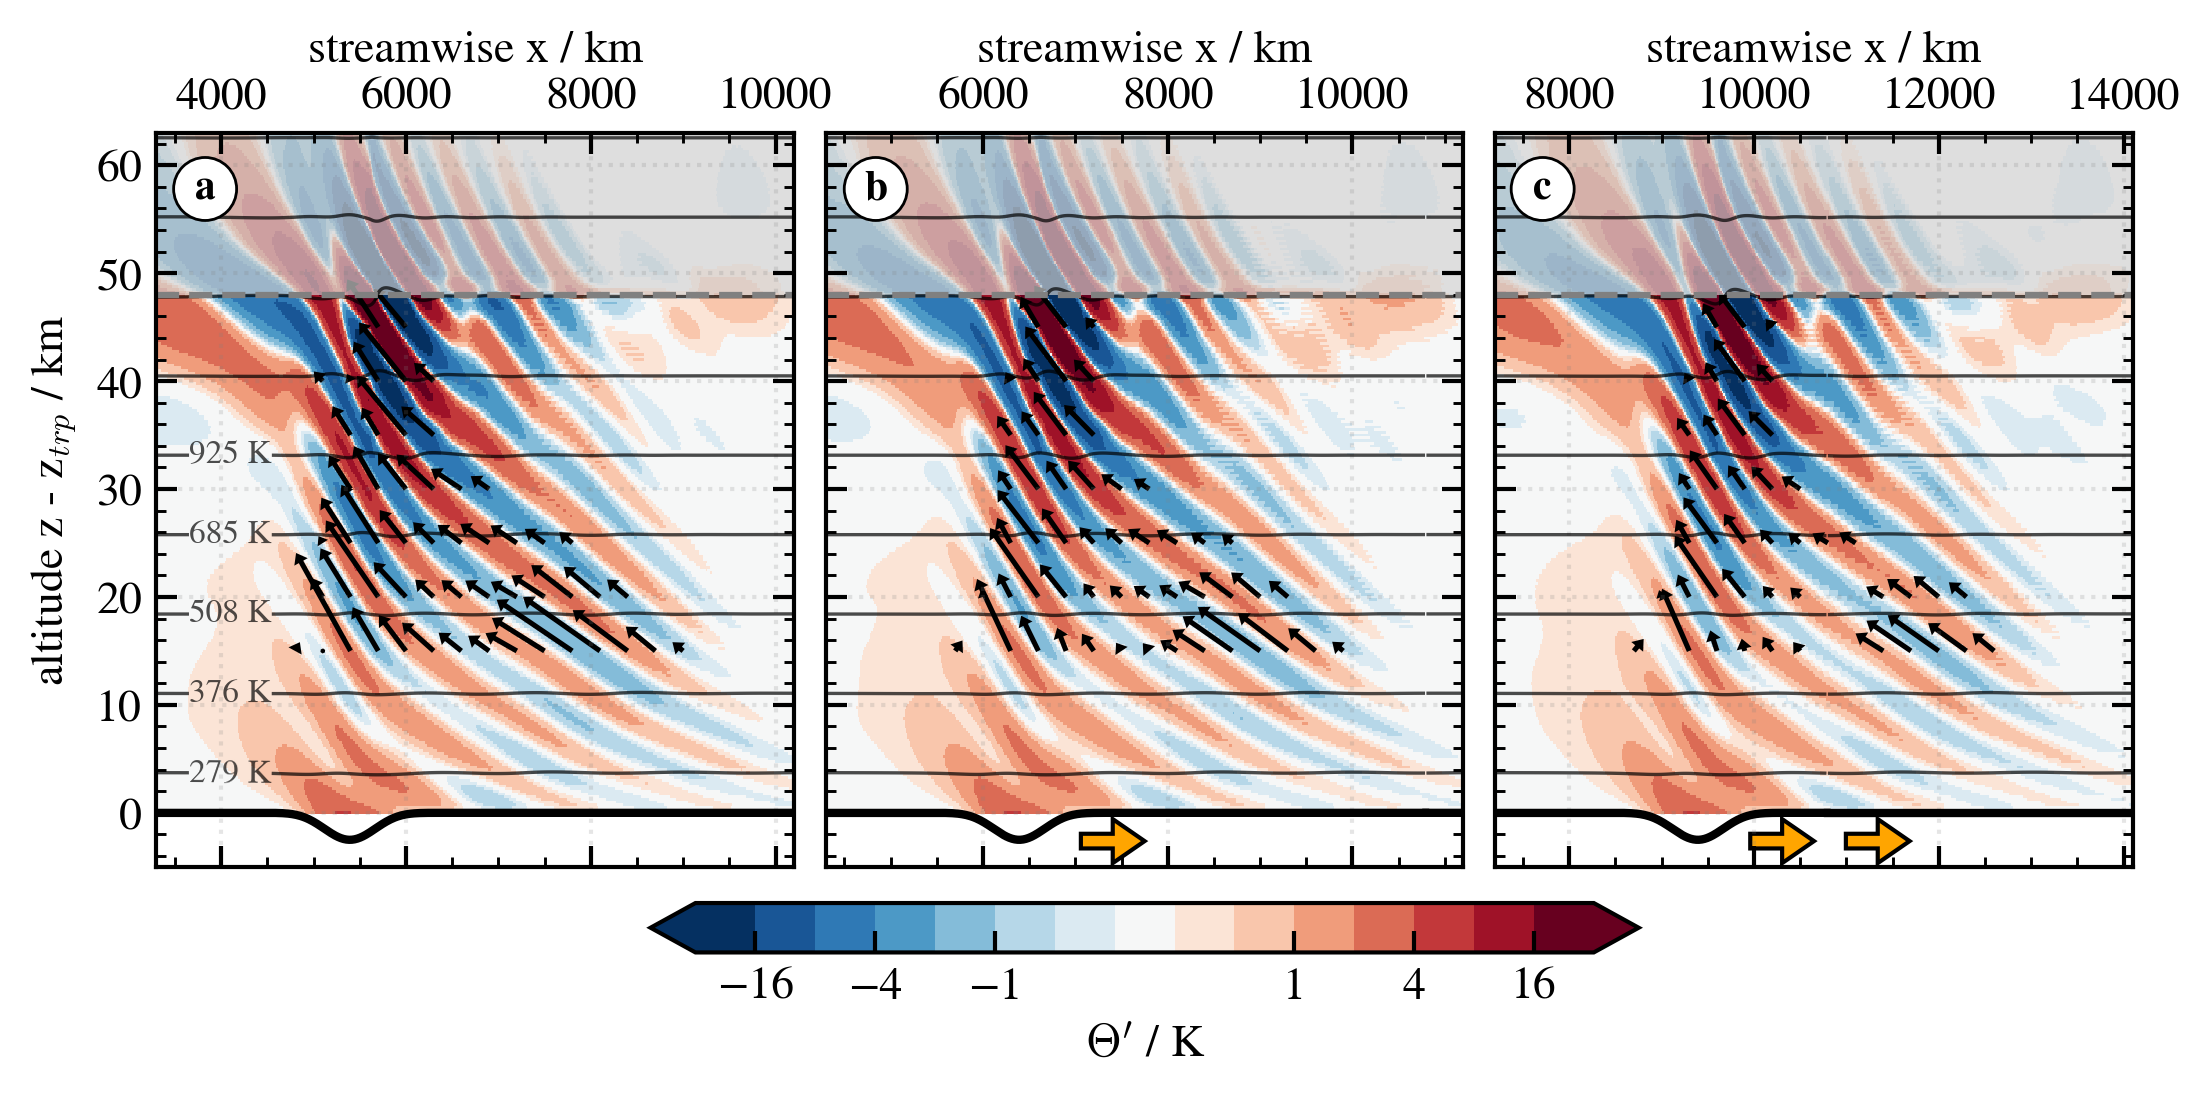
\includegraphics[width=0.99\textwidth]{figures_q3D/Q3D-TH-EF-ctropo.png}
    \caption{Shown are potential temperature perturbations $\Theta'$ overlayed by normalized vectors of \textbf{EF} for three different simulations with a constant background wind profile $u_e$ that corresponds to a $u_{e,MW}=\SI{31.12}{\meter\per\second}$. (a) represents the "MW case" with a stationary lower boundary. In (b) the tropopause fold moves with $c_{tf}$ and the backround wind is increased by $c_{tf}$. In (c) the tropopause fold moves with $2c_{tf}$ and again the backround wind is increased by $2c_{tf}$ with respect to (a). Note the different positions of the tropopause fold in streamwise direction after t=\SI{60}{\hour} and the strong similarity of all three simulations.}
    \label{fig:q3D_ctropo}
    % difference due to rising mountain?? 
\end{figure*}
We start with the propagation speed of the tropopause fold $c_{tf}$, because its relation to the background wind $u_e(z)$ is probably the most fundamental result of this chapter. Simulations with different $c_{tf}$ showed that the wave activity within a reference frame moving with the fold only depends on the relative difference between $u_e(z)$ and $c_{tf}$. Thus, it is possible to define a mountain wave wind speed
\begin{equation}
    u_{e,MW}(z) = u_e(z)-c_{tf}
    \label{equ:MW_forcing}
\end{equation}
that leads to an identical GW pattern with a stationary tropopause fold as in the propagating case. The complete vertical wind profile has to be reduced by $c_{tf}$ to achieve similar GWs. In other words, variations of the complete vertical profile $u_e(z)$ have a similar effect on the GW activity as variations of the fold's propagation speed. Figure \ref{fig:q3D_ctropo} visualizes an example showing three simulations with varying $u_e$ and $c_{tf}$, but a constant $u_{e,MW}=\SI{31.12}{\meter\per\second}$. The position of the tropopause fold after t=\SI{60}{\hour} is very different, but the GW field looks quite similar for all simulations. Minor differences in perturbations are most likely related to varying interactions with the vertical sponge layer due to $c_{tf}$. The energy flux \textbf{EF} overlayed in all three simulations (Figure \ref{fig:q3D_ctropo}) allows a similar conclusion. As expected, its direction is always parallel to the phase lines and the overall pattern for (a)-(c) in Figure \ref{fig:q3D_ctropo} is similar. Only magnitudes of \textbf{EF} vary slightly between simulations. \\
The conclusion of this finding might be quite instructive. Under the assumptions of the proposed excitation mechanism (tropopause fold mimics an obstacle for the stratospheric flow above like a mountain or valley at the surface) NOGWs above these propagating folds behave and propagate just like MWs within the reference frame of the propagating fold for $u_{e,MW}$. Therefore, known properties of MWs are transferable to NOGWs above tropopause folds, but nevertheless a concise investigation with a moving tropopause fold follows within the next sections and chapter \ref{sec:results3D}.
% Under the assumption of 
%
\section{The influence of the tropopause shape}
\label{sec:q3D-shape}
% This section is kept short. 
To simplify the qualitative analysis of parameter variations and also provide a quantitative overview on certain aspects, different simulations are primarily compared based on Figures \ref{fig:q3D_shape} and \ref{fig:q3D-wind}, which show vertical profiles of momentum and energy fluxes. This section focuses on Figure \ref{fig:q3D_shape} and the variation of the zonal width and the depth of the tropopause depression.

A smaller width of the depression naturally results in shorter horizontal wavelengths and, therefore, in higher momentum and energy fluxes as illustrated in (a)-(c) of Figure \ref{fig:q3D_shape}. This makes sense, because waves with smaller horizontal or vertical scales concentrate their energy in a smaller area. In addition, smaller wavelengths lead to a higher frequency and waves travel faster (e.g. \cite[]{gill_atmosphere-ocean_1982}). Both phenomena lead to higher momentum and energy fluxes. (a), for example, suggests that decreasing the zonal width by $\frac{1}{3}$ increases the angular momentum flux MF$_{x,ang}$ in the upper stratosphere ($z \approx \SI{30}{\kilo\meter}$) by a factor of 5-6 (purple dashed line vs. black solid line). Note that statements like "increasing" or "decreasing" will always refer to the amount of the fluxes independent of their sign. The sign indicates the direction of the flux. \\
In (b) EF$_z$ is about 6 times higher for $L=\SI{200}{\kilo\meter}$, too. As described in section \ref{sec:linear-MWs}, the Eliassen-Palm relation for rotating fluids from equation (\ref{equ:EP-relation-rotating}) states that MF$_{x,ang}$ and EF$_z$ are related via the background wind. A similar ratio between simulations for MF$_{x,ang}$ and EF$_z$ suggests that the EP relation is applicable. Furthermore, the vertical profile of the energy flux EF$_z$ nicely illustrates how wave energy is reduced in areas with negative shear (lower stratosphere) and produced in the positive shear of the PNJ (compare with Figure 6 of \textcite[]{eliassen_transfer_1960}). Physically, this variation of EF$_z$ can also be interpreted as a conversion of mean flow shear energy to wave energy flux (\cite[]{kruse_gravity_2015}). From a relative point of view, the production of EF$_z$ due to the PNJ (positive shear between 15 and \SI{40}{\kilo\meter}) is similar for $L=\SI{200}{\kilo\meter}$ and $L=\SI{300}{\kilo\meter}$. It is approximately \SI{70}{\percent}.

\begin{figure*}[t]
    \centering
    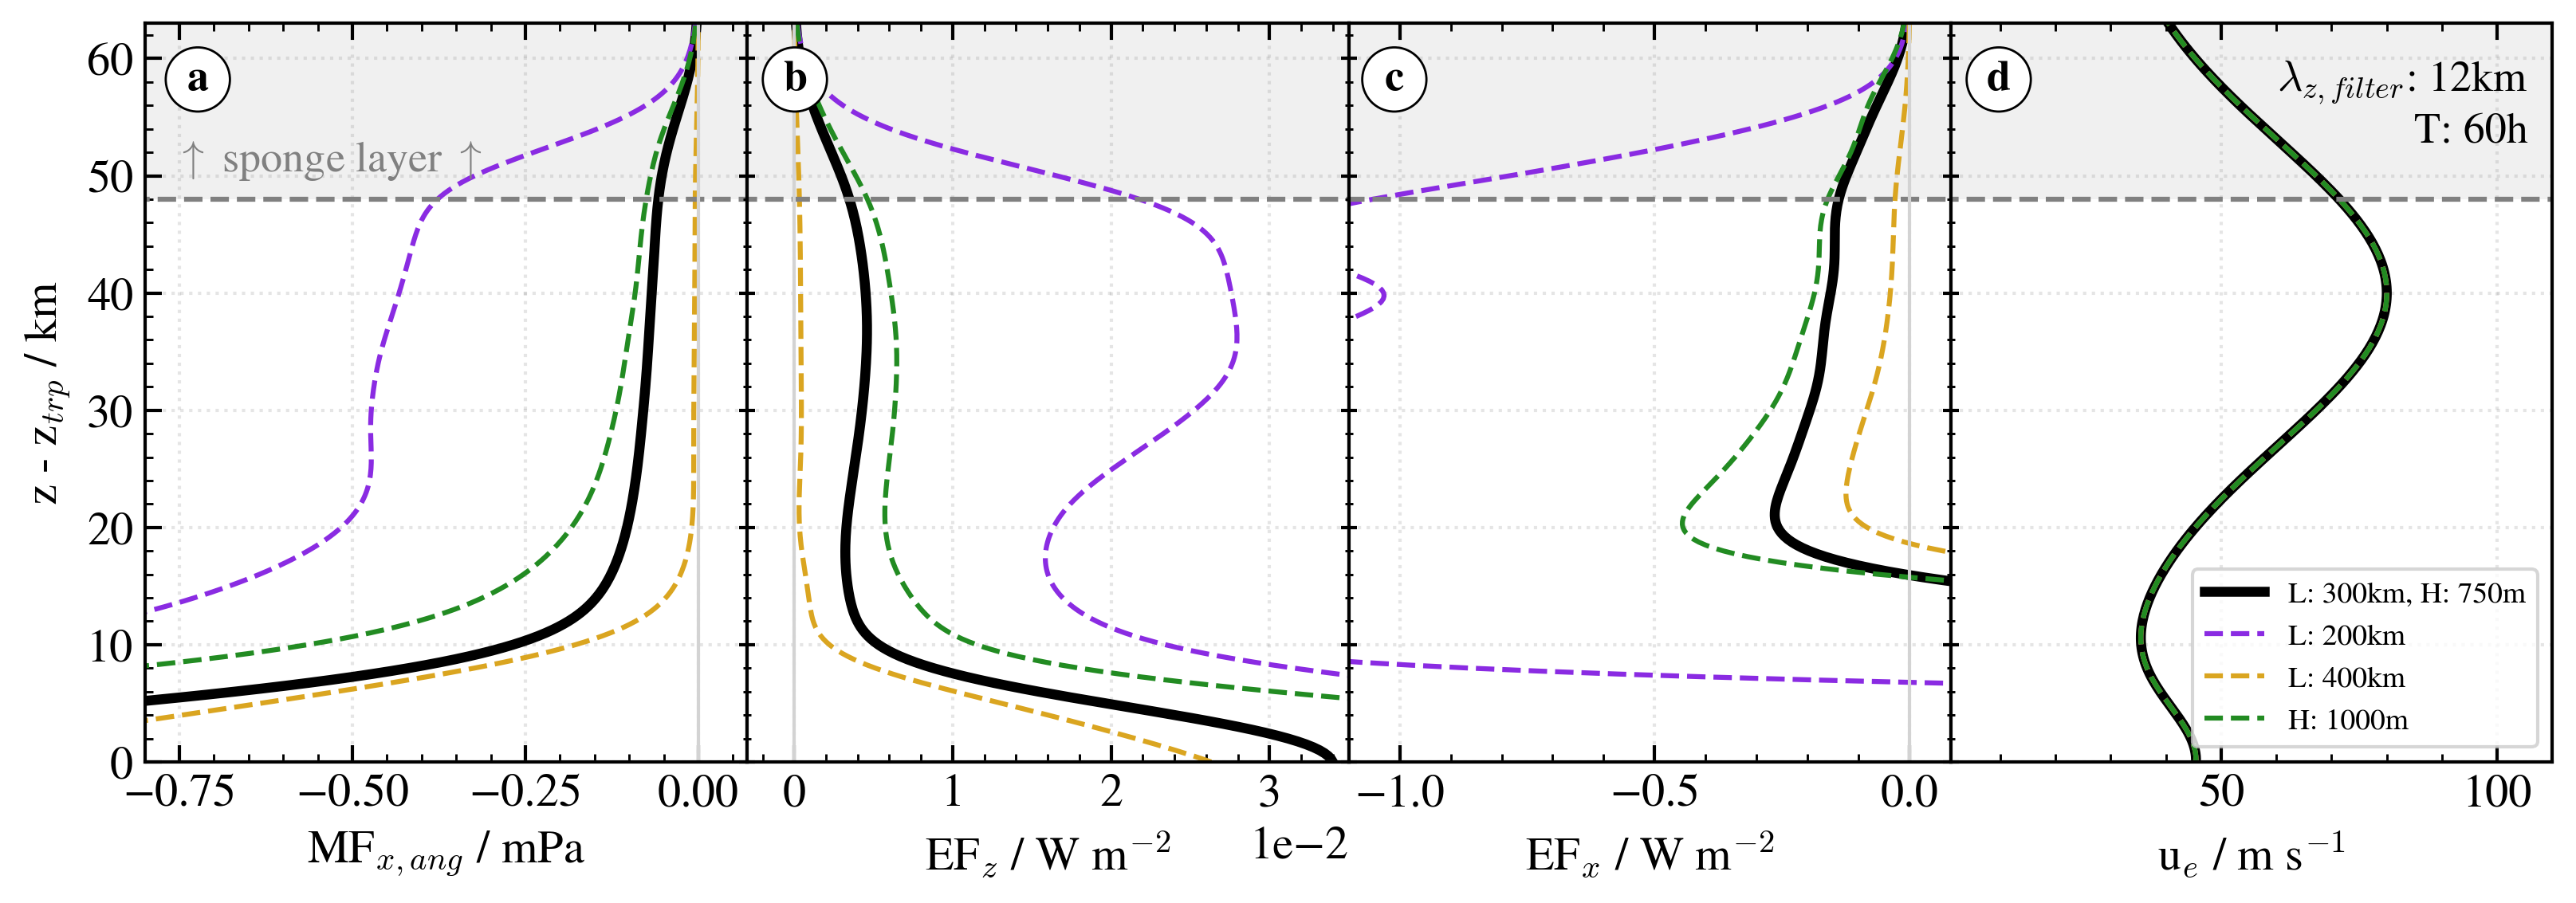
\includegraphics[width=0.99\textwidth]{figures_q3D/TD-zprofiles-translbq3D_shape-T60h-avg.png}
    \caption{Vertical profiles of zonal averages for the vertical flux of zonal angular momentum MF$_{x,ang}$ (a), the vertical energy flux EF$_z$ (b), the zonal energy flux EF$_x$ (c) and the ambient wind $u_e$ (d) for different simulations with a propagating tropopause fold. The thick black solid line represents the reference simulation from Figure \ref{fig:q3D_referenceSim} and dashed lines refer to variations of this simulation as stated in the legend of (d). All profiles are filtered in the vertical with a cutoff wavelength $\lambda_{z,filter}=\SI{12}{\kilo\meter}$. In this figure, all simulations utilize the same wind profile $u_e(z)$.}
    \label{fig:q3D_shape}
\end{figure*}
A larger depth of the tropopause fold increases all momentum and energy fluxes in Figure \ref{fig:q3D_shape}, because larger deflections at the tropopause increase perturbation amplitudes throughout the stratosphere. However, horizontal scales of the GWs, propagation speeds or the wave regime in general are not affected. The horizontal energy flux EF$_x$ in (c) depicts this most clearly. While variations of the depression width lead to different heights for the sign change of EF$_x$, the simulation with an increased depression depth has an identical height for the transition from positive to negative values of EF$_x$ as the reference simulation. The reason for this transition of EF$_x$ in the lower stratosphere is not fully understood. It is also observed for low frequency waves or IGWs and a constant wind profile during the model validation in section \ref{sec:linear-MWs}. Therefore, it seems to be related to rotational effects.
% 3D nature of IGWs and
%
\section{The influence of the stratospheric environment}
\label{sec:q3D-wind}
\begin{figure*}[t]
    \centering
    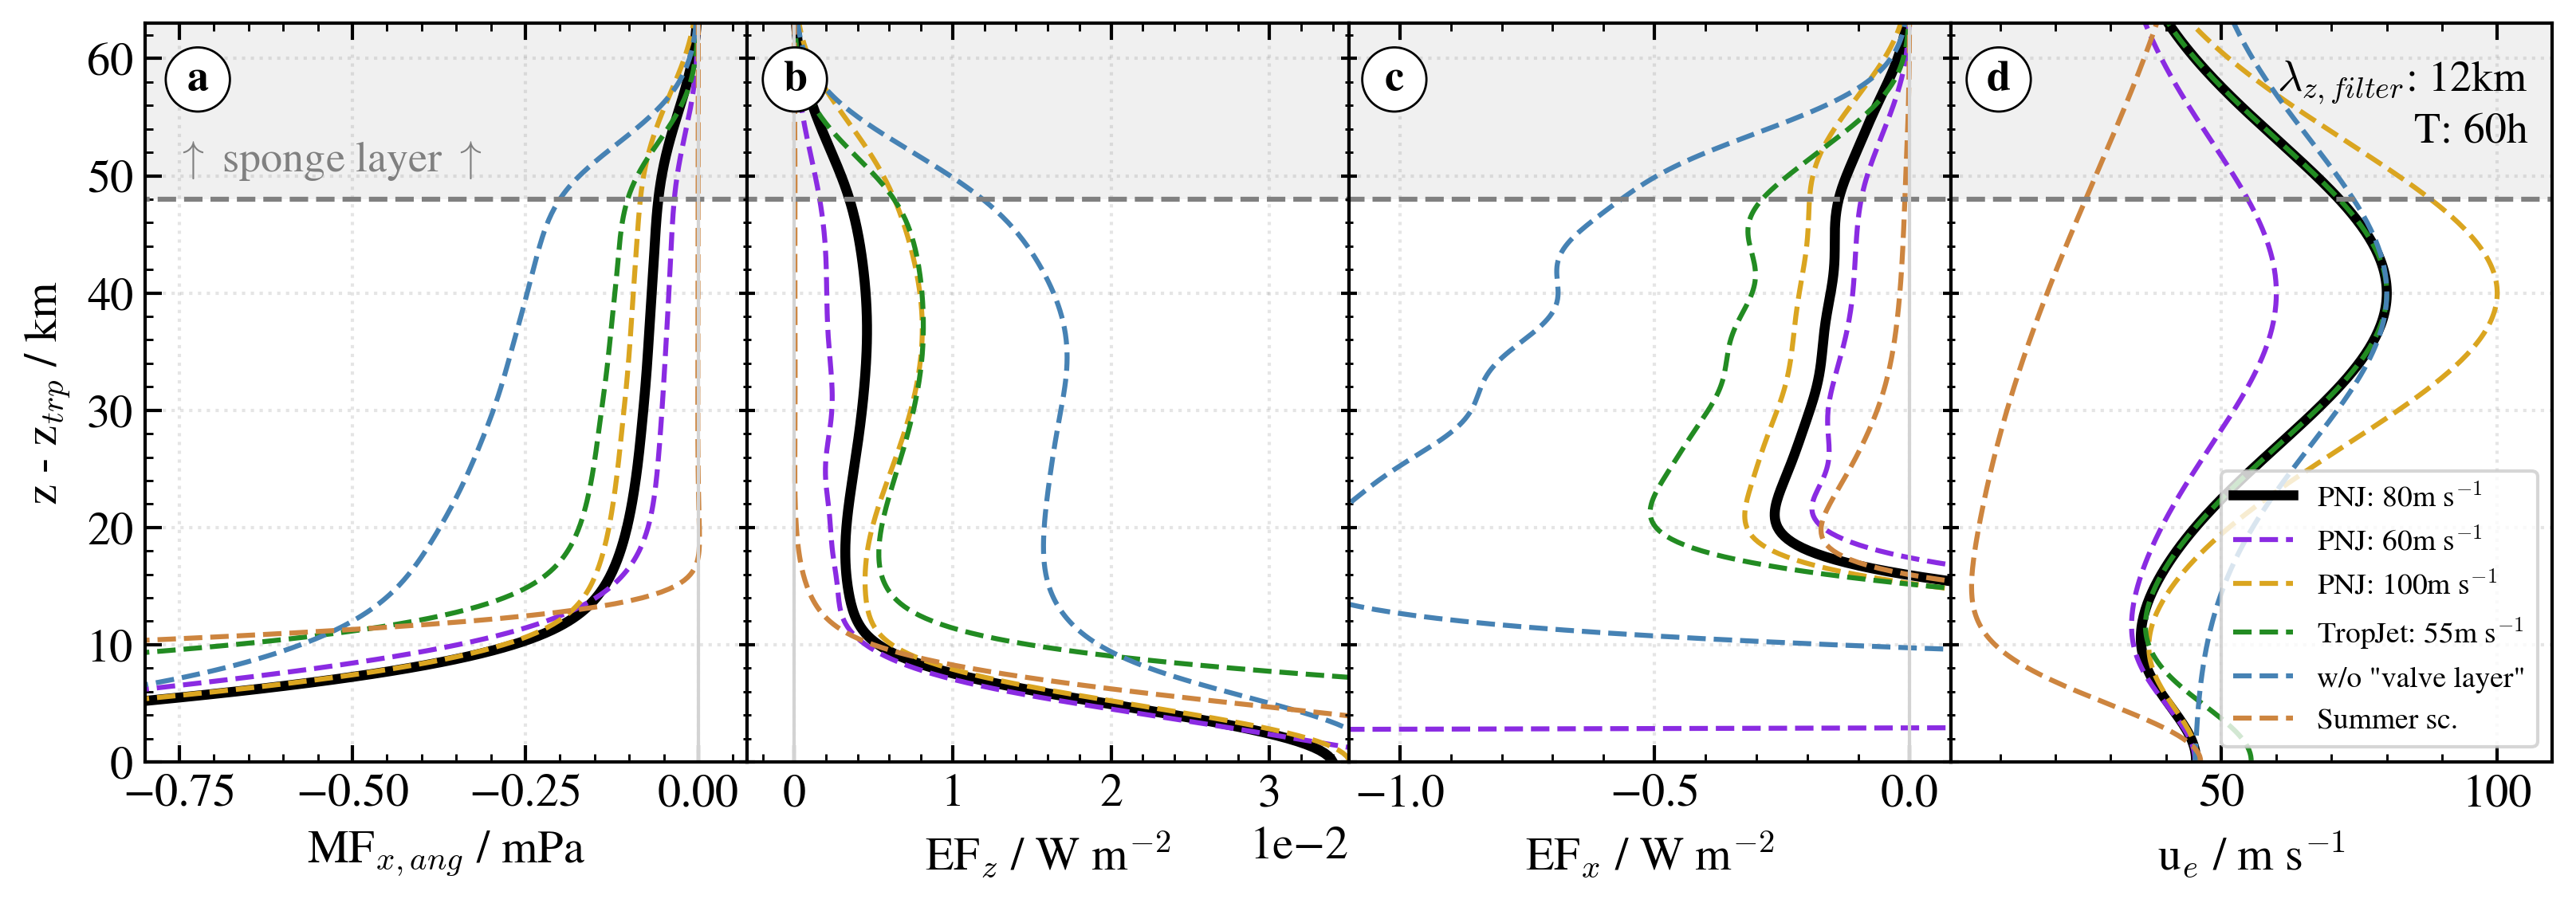
\includegraphics[width=0.99\textwidth]{figures_q3D/TD-zprofiles-translbq3D_wind-T60h-avg.png}
    \caption{Similar to Figure \ref{fig:q3D_shape}, but simulations utilze different wind profiles as indicated in (d). All other parameters of the simulations are identical to the reference simulation.}
    \label{fig:q3D_wind}
\end{figure*}
The main focus of this section is on the comparison of different ambient wind profiles presented in Figure \ref{fig:q3D_wind}d. A brief discussion of simulations with varying Coriolis parameter and stratification is found at the end.

The dashed purple and yellow lines in Figure \ref{fig:q3D_wind} represent simulations with a weaker ($u_{PNJ,max}$=\SI{60}{\meter\per\second}) and stronger ($u_{PNJ,max}$=\SI{100}{\meter\per\second}) PNJ. The tropopause jet (TPJ) at lower altitudes is the same for these simulations. As expected, momentum and energy fluxes look almost identical up to approximately $z$=\SI{15}{\kilo\meter}, but deviate in the upper stratosphere. Stronger winds lead to stronger momentum and energy fluxes. An increase of EF$_z$ due to the stronger shear of the PNJ is consistent with the discussion on wind shear and energy production in the previous section, but higher momentum fluxes are caused differently. As derived in the model validation section \ref{sec:linear-MWs} the vertical flux of angular momentum MF$_{x,ang}$ should be similar for all simulations with the same forcing at tropopause level and for conservative wave propagation. Here, the propagation of waves is not conservative due to the negative shear above the TPJ and the resulting wind minimum at $z$=10-\SI{12}{\kilo\meter}. In this so-called "valve layer" nonlinear processes irreversibly dissipate momentum and influence the momentum flux above (\cite[]{kruse_midlatitude_2016}). A close observation of the three relevant wind profiles reveals that the negative shear and the wind minimum of the valve layer is more pronounced for the weaker PNJ (dashed purple line). Therefore, more momentum is attenuated and MF$_{x,ang}$ becomes smaller in the upper stratosphere.

\begin{figure*}[t]
    \centering
    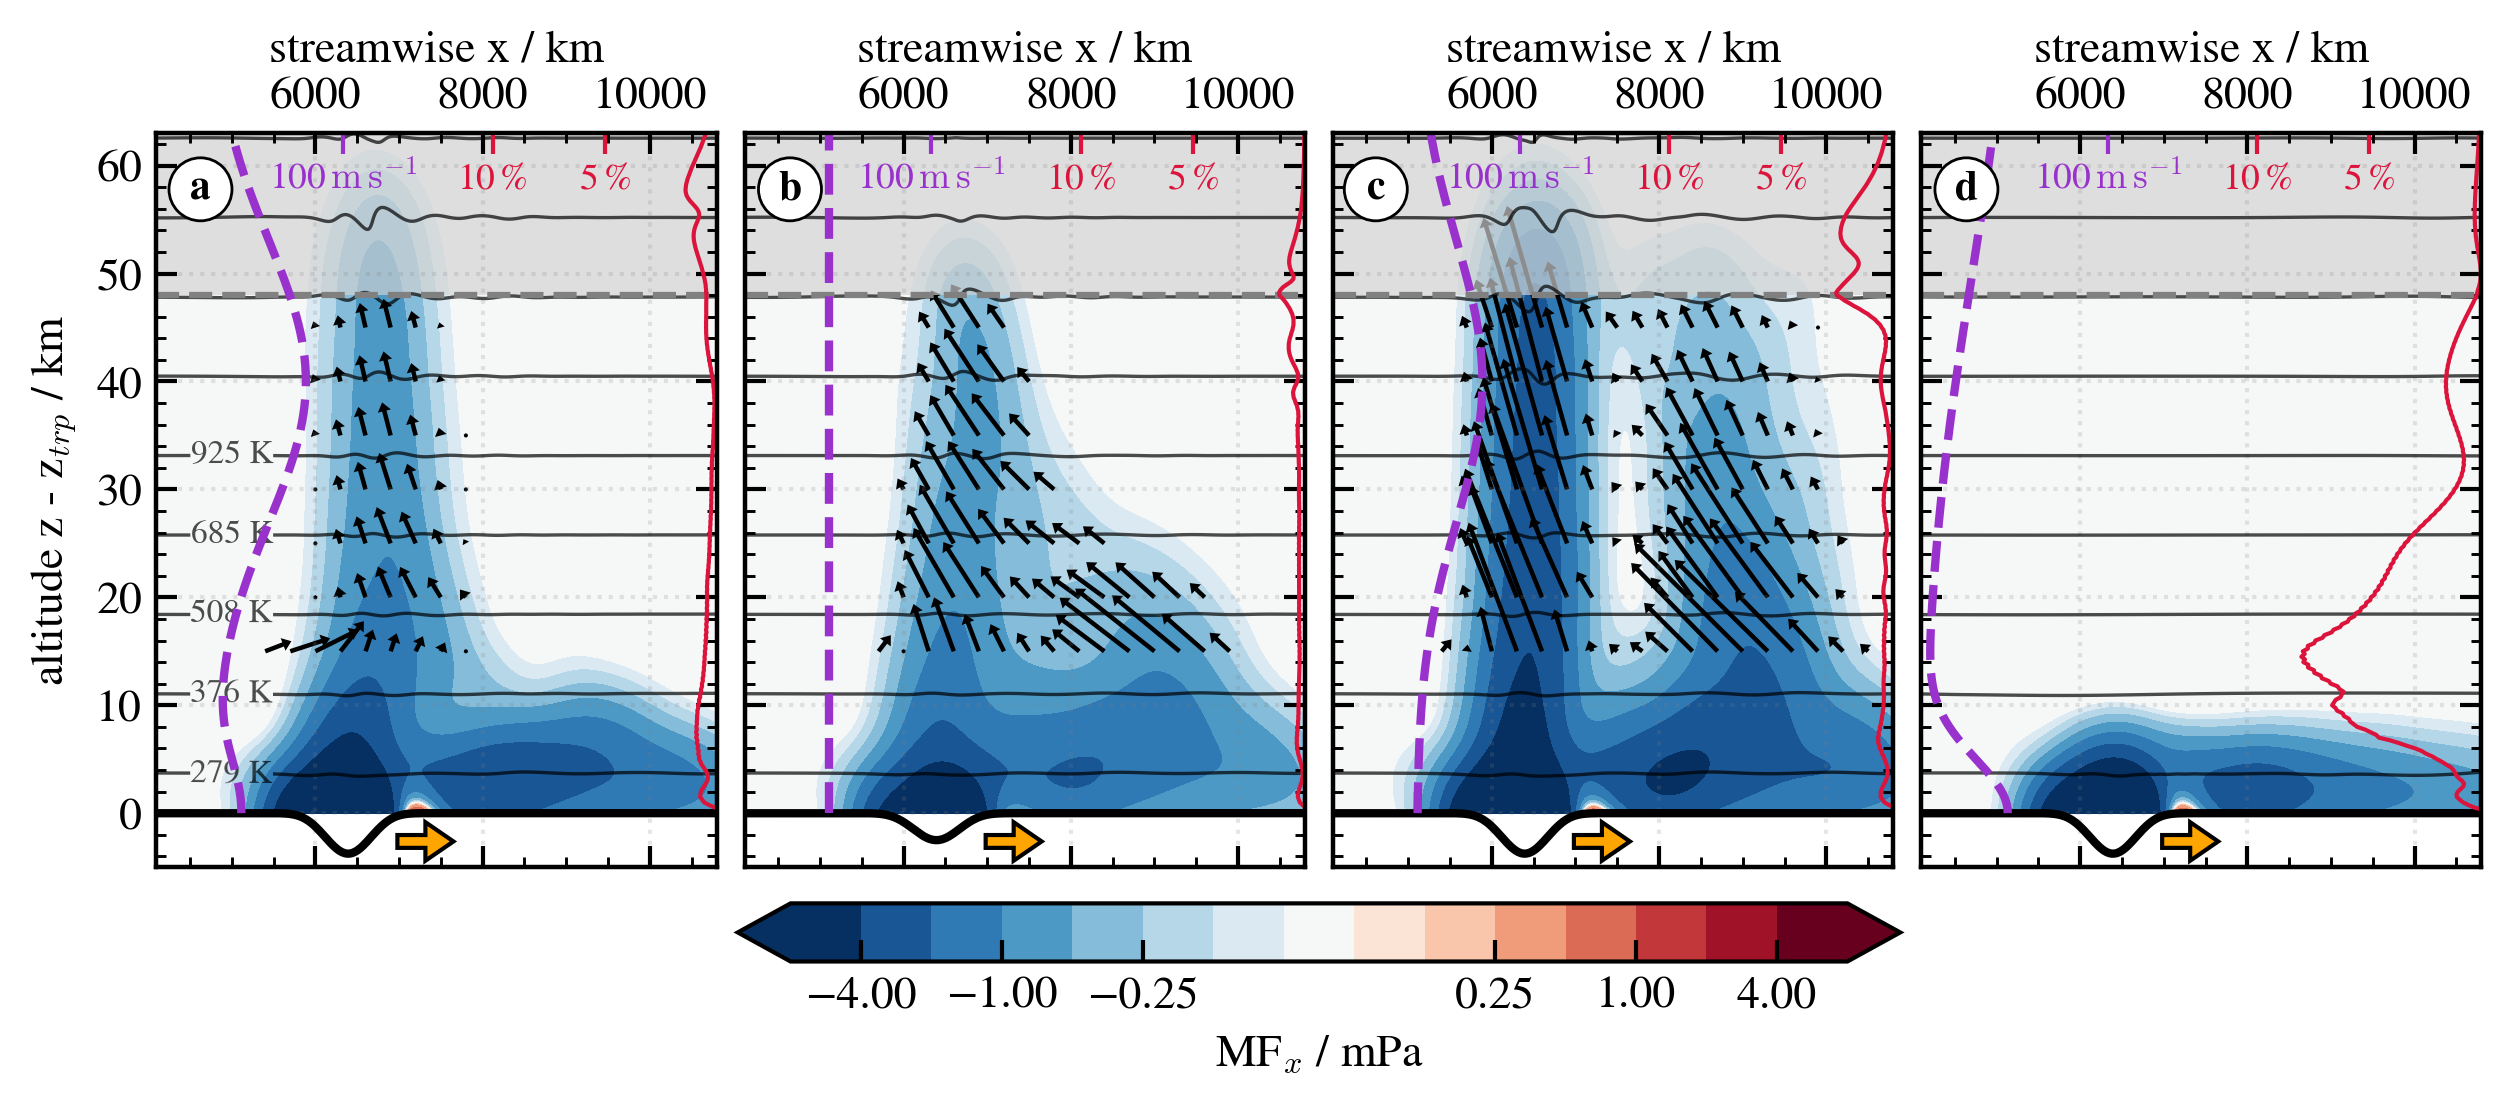
\includegraphics[width=0.99\textwidth]{figures_q3D/Q3D-MFx-towers.png}
    \caption{Cross sections at y=0 and t=\SI{60}{\hour} showing the vertical flux of zonal momentum (MF$_x$) for four different simulations. (a) is the reference simulation, (b) has a stronger PNJ with $u_{max}=\SI{100}{\meter\per\second}$, (c) has no valve layer (wind minimum above the tropopause jet) and (d) represents the summer scenario without a PNJ. Fluxes are averaged with a Gaussian filter according to \textcite[]{kruse_gravity_2015} and black arrows indicate the normalized vector of the energy flux \textbf{EF}.}
    \label{fig:q3D-mfx-towers}
\end{figure*}
The effect of the valve layer becomes much more apparent when comparing the reference simulation to a simulation without a valve layer (dashed blue lines) and the summer scenario for the southern hemisphere stratosphere (dashed red lines in Figure \ref{fig:q3D_wind}). For the blue simulation, maximum speeds of the TPJ and PNJ stay the same, but the valve layer has been removed. For the red simulation, the PNJ is removed and the wind minimum is further reduced, but the wind speed at tropopause level is still the same as in the reference simulation. The momentum and energy fluxes present a consistent picture. Removing the valve layer results in far bigger momentum and energy fluxes compared to all other simulations, removing the PNJ and further decreasing the wind speed of the valve layer leads to vanishing fluxes in the upper stratosphere. Vertical cross sections of MF$_x$ for these simulations further illustrate these features in Figure \ref{fig:q3D-mfx-towers}. In simulations (a) to (c) large values of MF$_x$ reach high up into the upper stratosphere, but for the summer scenario in (d) MF$_x$ disappears above $z$=\SI{10}{\kilo\meter}. \textcite[]{kruse_gravity_2015} called these patterns of high-reaching momentum flux in (a),(b) and (c) flux towers and, again, in the simulation without a valve layer in (c) the tower is much more pronounced compared to the reference simulation (a) or the simulation with a stronger PNJ (b). How can we explain these different flux towers and varying profiles of MF$_{x,ang}$, if linear theory expects vertical vaariations of momentum flux only in the context of critical levels or reflection layers (\cite[]{booker_critical_1967}, \cite[]{jones_propagation_1967} and \cite[]{broad_linear_1995})? \\
At first, we note that wave reflection in the presence of the PNJ is only relevant for horizontal wavelenghts below 30-\SI{40}{\kilo\meter} and can be ruled out for the scales of GWs above tropopause folds (\cite[]{gill_atmosphere-ocean_1982} or \cite[]{mixa_nonlinear_2021}). Furthermore, a slight decrease of MF$_{x,ang}$ with height is already observed for EULAG simulations with a constant wind profile in Section \ref{sec:linear-MWs}, but the decrease observed in simulations of this section with vertical shear is much more pronounced and suggests the presence of critical levels. In a 2D flow an internal GW reaches its critical level $z_c$ when its horizontal phase speed is equal to the background wind. In a 3D rotating fluid with purely zonal background flow (V=0) a critical level is defined for 
\begin{equation}
    \omega - Uk = \hat{\omega} = f,
    \label{equ:critical_level}
\end{equation}
so the intrinsic frequency $\hat{\omega}$ does not vanish, but approaches the Coriolis frequency $f$ and the GW becomes an inertial oscillation (\cite{jones_propagation_1967}). At the same time, the vertical wavelength and group velocity of the GW decrease to 0 at $z_c$ (e.g. \cite[]{lin_mesoscale_2007}). Based on the results from Section \ref{sec:q3D-speed} the horizontal phase speed of NOGWs above propagating tropopause depressions is not 0 as for stationary MWs, but equal to the propagation speed of the depression $c_{p,x}=c_{tf}=\SI{13.88}{\meter\per\second}$. In other words, GWs propagate like MWs within the moving reference frame of the depression. Consequently, the vertical wind profile of the summer scenario in Figure \ref{fig:q3D_wind} and \ref{fig:q3D-mfx-towers} clearly contains a critical level for the excited GWs (wind speed drops below $c_{tf}$) and it is plausible that the flux tower completely disappears in Figure \ref{fig:q3D-mfx-towers}d. However, the wind minimum of the reference simulation or the simulation with an increased PNJ is approximately \SI{35}{\meter\per\second}, so much greater than the wind speed at a critical level, which would be slightly higher than $c_{tf}$. Now, one way to interpret the momentum flux variation with height in these simulations is the valve layer mentioned above. Though linear theory predicts wave dissipation only at the critical level $z_c$, in reality, it takes an infinite time for a GW to actually reach its critical level, because its vertical group velocity and vertical wavelength vanish. Therefore, GW dissipation due to a critical level could be understood as a continuous process that starts as soon as a GW approaches its critical level. In the case of MWs or NOGWs above tropopause depressions, a decreasing background wind with height is synonymous to approaching a critical level, which is consistent with \textcite[]{kruse_midlatitude_2016}'s description of a valve layer: A layer of reduced wind speed with no wind reversal or critical level. \\
\textcite[]{bretherton_propagation_1966} or \textcite[]{booker_critical_1967} conclude from their analysis (W.K.B approximation) that the flow regime and processes effecting the momentum and energy fluxes can be related to the gradient Richardson number $R_i=\frac{N^2}{\frac{\partial U}{\partial z}}$, but admit that their linear analysis is limited in the vicinity of critical levels. A few years later, nonlinear numerical simulations by \textcite[]{breeding_non-linear_1971} revealed three flow regimes for $R_i \leq \frac{1}{4}$, $\frac{1}{4} < R_i < 2$ and $R_i \geq 2$.
\begin{wrapfigure}{r}{6cm}
    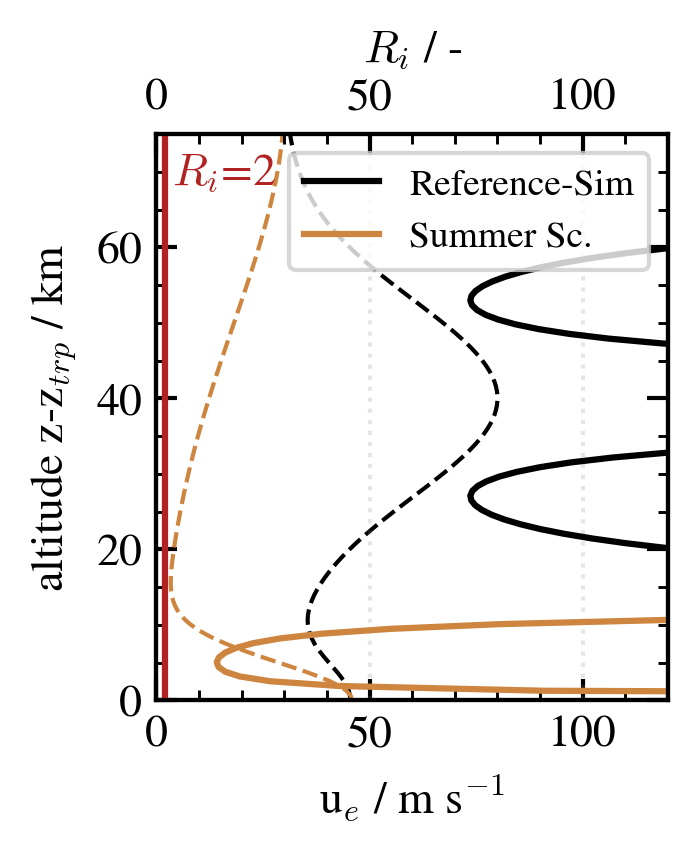
\includegraphics[width=6cm]{figures_q3D/critical-layer-ana.png}
    \caption{Wind profiles (dashed lines) and Richardson number $R_i$ (solid lines) for the reference simulation (black) and the summer scenario (reddish). The vertical red line indicates $R_i=2$.}
    % \vspace{-110pt} % This removes the white box on the second page
    \label{fig:ri}
\end{wrapfigure}
For the latter, very little of the GW penetrates through the critical level and almost all of the wave's energy and momentum is reabsorbed by the mean flow without necessarily invoking turbulence or other dissipative processes (\cite[]{booker_critical_1967}). Figure \ref{fig:ri} illustrates that $R_i >> 2$ holds for all levels of the reference simulation and the summer scenario with a much stronger negative shear above the TPJ, so we can conclude that the valve layer (negative shear above the tropopause jet) is responsible for decreasing MF$_{x,ang}$ in Figure \ref{fig:q3D_wind} due to absorption of energy and momentum by the mean flow.  

A last variation of the ambient wind profile in Figure \ref{fig:q3D_wind} is a stronger TPJ (green dashed lines). The wind speed at tropopause level is increased by \SI{10}{\meter\per\second}, but the wind minimum above is almost similar to the reference simulation. As expected, MF$_{x,ang}$ is larger in the lower stratosphere, but it is also more pronounced in the upper stratosphere. Though the negative shear above the TPJ is stronger, more momentum can pass through the valve layer. The momentum flux in the upper stratosphere is also higher compared to the simulation with a stronger PNJ (dashed yellow line in Figure \ref{fig:q3D_wind}), but a higher energy production in the positive shear of the PNJ compesates for the smaller momentum flux. Increasing the TPJ by \SI{10}{\meter\per\second} had exactly the same effect on upper level EF$_z$ as increasing the PNJ by \SI{20}{\meter\per\second}. From a quantitative point of view, GW activity in the upper stratosphere seems to be more sensitive to the ambient wind at excitation level (tropopause) as to the flow at upper levels.

Simulations with varying Coriolis parameter or stratification have also been conducted, but not presented in the figures. When decreasing the Coriolis parameter, so it corresponds to a latitude of \SI{45}{\degree S}, all momentum and energy fluxes increase and we observe a lower transition from positive to negative values for EF$_x$. On the contrary, reducing the Brunt-Väisälä frequency to $N=\SI{0.015}{\per\second}$ leads to marginal changes in the momentum and energy fluxes, because density and potential temperature profiles are coupled in the Bacmeister-Schoeberl model.

%%%%%%%%%%%%%%%
% However, these changes in the wind are centred above the critical level, so that the change in the wind has only a small effect on the height of the critical level

% Thus the packet is neither transmitted nor reflected - it simply slows down until either viscosity, turbulence or other non-linearities destroy it as a coherent entity.

% kruse 2016
% Such a layer might allow small-amplitude mountain waves to be trans- mitted unaffected but might also cause larger-amplitude mountain waves to steepen, become nonlinear, and attenuate 

% Another view relates energy fluxes and valve layer  via group velocity also slows down the GW propagation (reduces group velovcity)

% \cite[]{dornbrack_evidence_2002} waves over scandinavia
% convective instability vs. shear instability 

% 3D critical levels!! \cite[]{teixeira_momentum_2009}
% However, the interest for flows with directional shear and critical layers (where the wave momentum is deposited over a continuous range of heights, as opposed to critical levels) has increased recently, since these flows are much more realistic

% For a directionally sheared flow and a 3D mountain, there is no single critical level, but a distribution of them with height, depending on the wavenumber of the gravity waves (i.e., a critical layer). This study aims to calculate the momentum flux in such situations of directional shear and 3D orography, addressed first by SG99

% According to Eliassen and Palm [1960] for linear, steady, small-amplitude, non-dissipative MW

% Fritts 2003
%Dissipation results from processes such as radiative damping [Fels, 1984; Zhu, 1994], wave–wave and wavemean flow interactions [Broutman and Grimshaw, 1988; Sutherland, 2000, 2001], and wave breaking and instability processes (see section 6).
%%%%%%%%%%%

%%%%%
% Vertical wavelenghts increase proportional to zonal cross sections and energy fluxes increase for stronger wind

% \begin{equation}
%     c_{gx} \approx \frac{N^2 \alpha}{m \sqrt{f^2+N^2 \alpha^2}} \approx \SI{-26.9}{\meter\per\second} 
% \end{equation}
% with a negative $m$ for upward propagating waves and the vertical group velocity
% \begin{equation}
%     c_{gz} \approx -\alpha c_{gx} \approx \SI{0.36}{\meter\per\second}
%     % \label{equ_lid:cgz}
% \end{equation}
%
% \section{Influence of Coriolis force and stratification}
% \begin{figure*}[t]
%     \centering
%     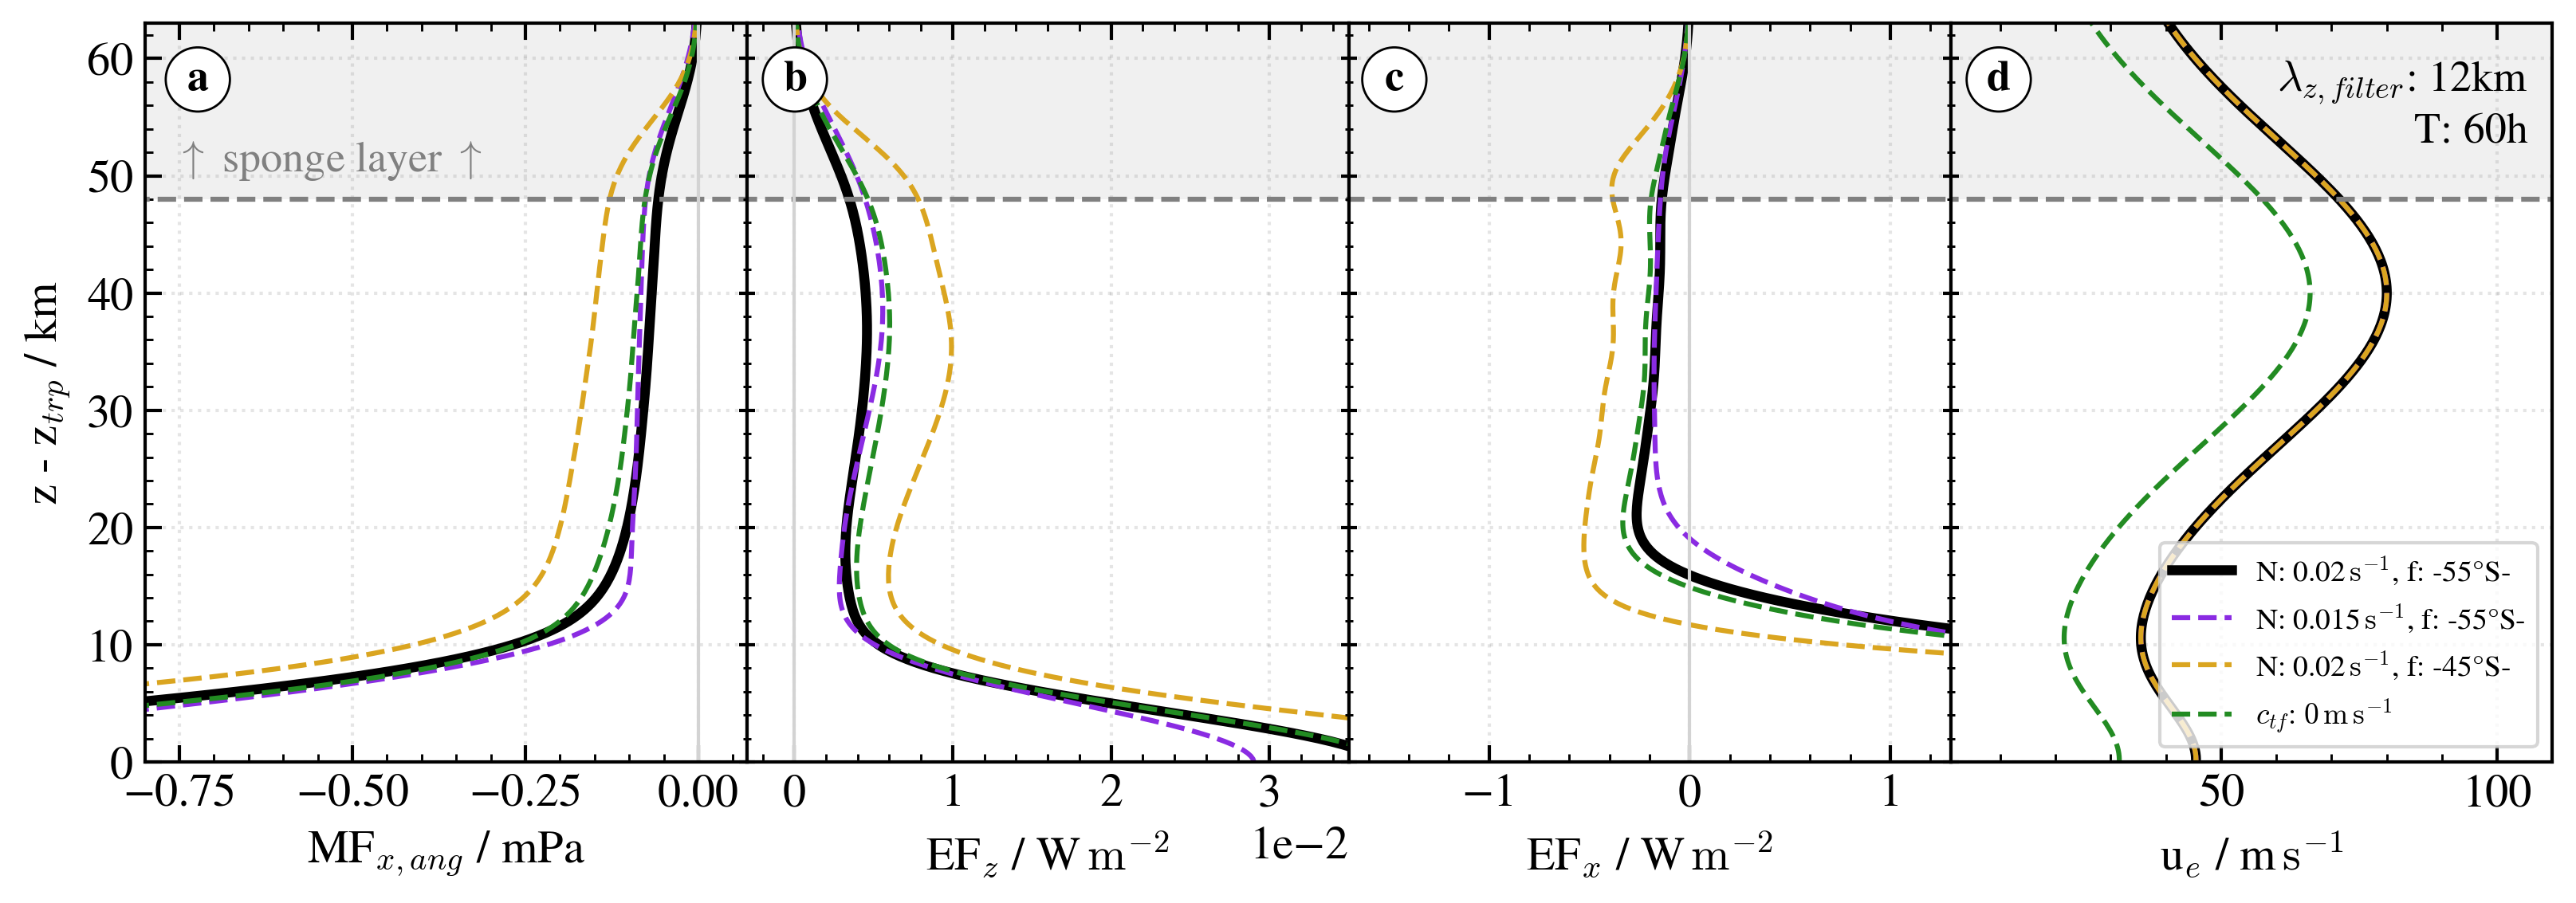
\includegraphics[width=0.99\textwidth]{figures_q3D/TD-zprofiles-translbq3D_atm-T60h-avg.png}
%     \caption{Similar to Figure \ref{fig:q3D_shape} and Figure \ref{fig:q3D_wind}, but simulations vary the Coriolis paramter $f$, the Brunt-Väisälä frequency $N$ and the propagation speed $c_{tf}$. All other parameters of the simulations are identical to the reference simulation.}
%     \label{fig:q3D_atm}
% \end{figure*}

\section{Summary and answer to research question (R1)}
\label{sec:q3D-summary}
The objective of this chapter was to identify zonal and vertical properties of the tropopause (width and height of a depression) and the stratospheric environment (e.g. variation of the ambient wind profile) that significantly influence the GW activity in the upper stratosphere to answer the research question
\begin{tcolorbox}[]
    (R1) How sensitive are NOGWs from propagating tropopause depressions to the depression's 2D shape and to 2D properties of the stratospheric environment?
    % How are NOGWs effected by ...
    % (R2) How sensitive are NOGWs from propagating tropopause folds to the 2D shape of the depression and the stratospheric environment?
\end{tcolorbox}
Under the assumption that the tropopause can be emulated by a transient, impermeable and frictionless lower boundary in the numerical simulations, a fundamental result of the analysis came out of Section \ref{sec:q3D-speed}. Varying the propagation speed of the tropopause depression $c_{tf}$ has a similar effect as varying the whole vertical profile of the ambient wind. So NOGWs above tropopause depressions behave and propagate just like MWs within the reference frame of the propagating depression for a relative wind $u_{e,MW}$ (Equation (\ref{equ:MW_forcing})). \\
Furthermore, the presented simulations suggest the following qualitative conclusions for the sensitivity of NOGWs excited above propagating tropopause depressions:
\begin{itemize}
    \item Naturally, the GW activity in the upper stratosphere is proportional to the depth $H$ and inversely proportional to the half width $L$ of the tropopause depression.
    \item GW activity also increases for a stronger background wind speed $u_e(z)$ with a higher sensitivity for wind speeds in the lower stratosphere (tropopause jet) compared to the PNJ higher up.
    \item A pronounced stratospheric wind minimum has the largest effect on upper stratosphere GW activity (valve layer-like effect). Removing the valve layer without increasing the maximum wind speeds of the jet streams increases the GW activity in the upper stratosphere the most. 
    \item Introducing weak winds above the tropopause jet (summer scenario of southern hemisphere stratosphere) completely suppresses GW activity in the upper stratosphere. GWs already dissipate at lower levels due to a critical level that exists for $u_e \leq c_{tf}$.
    \item Decreasing the Coriolis force enhances the GW activity in the whole stratosphere.
\end{itemize}
Another informative test could be the variation of the vertical width $\sigma$ in Equation \ref{equ:wind-distribution} of the TPJ or the PNJ to increase (or decrease) the vertical shear without removing the valve layer completely, but it is omitted within the framework of this thesis. \\
The simulations presented in this chapter were conducted in 3D to correctly incorporate the Coriolis force. However, ambient conditions like the background wind were constant in meridional direction, so these simulations basically describe a scenario with the PNJ directly centered above the tropopause depression. In reality, the PNJ is often observed south of the storm track and corresponding tropopause folds during austral winter. The analysis in the next chapter deals with this situation and investigates the impact of meridional properties on the GW activity in the upper stratosphere.
\newpage
\thispagestyle{plain}

% ==== CHAPTER 5 ==============================================================
% ---- set some counters to zero:
\setcounter{equation}{0}
\setcounter{table}{0}
\setcounter{figure}{0}
% ---- include tex-file:
\chapter{NOGWs excited by tropopause depressions in 3D}
\label{sec:results3D}
3D simulations of the previous section focused on the analysis of zonal and vertical properties of the tropopause and stratosphere with a low grid resolution in meridional direction. However, it is clear that in most cases the shape of a tropopause depression varies meridionally and the PNJ is not centered above the depression. Meridional processes are important and significantly influence the appearance of GWs in the upper stratopshere. Therefore, this section presents full 3D simulations with an identical resolution in streamwise and spanwise direction and with meridional gradients. \\
Subsequent to Chapter \ref{sec:resultsq3D}, it is the goal to address the sensitivity of NOGWs above tropopause depressions to meridional properties of the tropopause and stratosphere by investigating the second research question
\begin{tcolorbox}[]
    (R2) How sensitive are NOGWs from propagating tropopause depressions to the depression's 3D shape and 3D properties of the stratospheric environment?
\end{tcolorbox}
In addition, realistic simulations of the stratosphere facilitate the investigation of the third research question, which refers to the zonally elongated phase lines in the horizontal cross sections of Figure \ref{fig:RF25_era5_horizonal}.
\begin{tcolorbox}[]
    (R3) Can NOGWs above propagating tropopause depressions explain the zonally elongated phase lines in ERA5 above the Southern Ocean?
    % the zonally elongated phase lines in the horizontal cross sections of Figure \ref{fig:RF25_era5_horizonal}. 
    % long vertical wave lengths in vertical cross section and elongated phase line in horizontal
\end{tcolorbox} 
All simulations of this chapter have the same temporal resolution (dt=\SI{60}{\second}) as simulations of Chapter \ref{sec:resultsQ3D}, but the horizontal and vertical domain is adapted to (n$_z$,n$_y$,n$_x$)=(251,480,720) grid points with a resolution of (dz,dy,dx)=(\SI{300}{\meter},\SI{20}{\kilo\meter},\SI{20}{\kilo\meter}). Again, periodic boundaries are used streamwise, linear sponge layers are used spanwise and the exponential sponge layer described in the "lessons learned" of Section \ref{sec:linear-MWs} is used vertically.

Two processes lead to a meridional propagation of GWs. The first process is solely caused by the 3D shape of the obstacle and becomes relevant as soon as the obstacle's shape changes in spanwise direction. The flow is not only deflected vertically, but also horizontally (flow around the isolated obstacle), which can result in a relevant lateral propagation of GWs. If, in addition, the shape is not symmetric in spanwise direction (e.g. a tilted tropopause depression with respect to the incoming flow), most of the GW activity might be channeled towards one side of the obstacle. Section \ref{sec:3D_noshear} analyses this process by comparing two simulations with different orientations of the tropopause depression in an environment without meridional wind shear. \\
The second process that leads to a meridional propagation of GWs is the modification of the wave-vector by meridional wind shear. Since this process is also linked to the depression's shape, Section \ref{sec:3D_shear} discusses variations of the background wind and Section \ref{sec:3D_shape} deals with variations of the depression's shape in the presence of meridional shear. \\
It follows a comparison of common methods to calculate the momentum flux from observations and from simulations in Section \ref{sec:3D_mf} and a short summary of the chapter in Section \ref{sec:3D_summary}.

% 3D orientation of wave-vector
% meridional propagation / meridional component of the wave vector can 

%%% No meridional shear %%%%
% \section{The influence of rotating the tropopause depression}
\section{The influence of the tropopause shape in the context of no meridional shear}
\label{sec:3D_noshear}
\begin{figure*}[t]
    \centering
    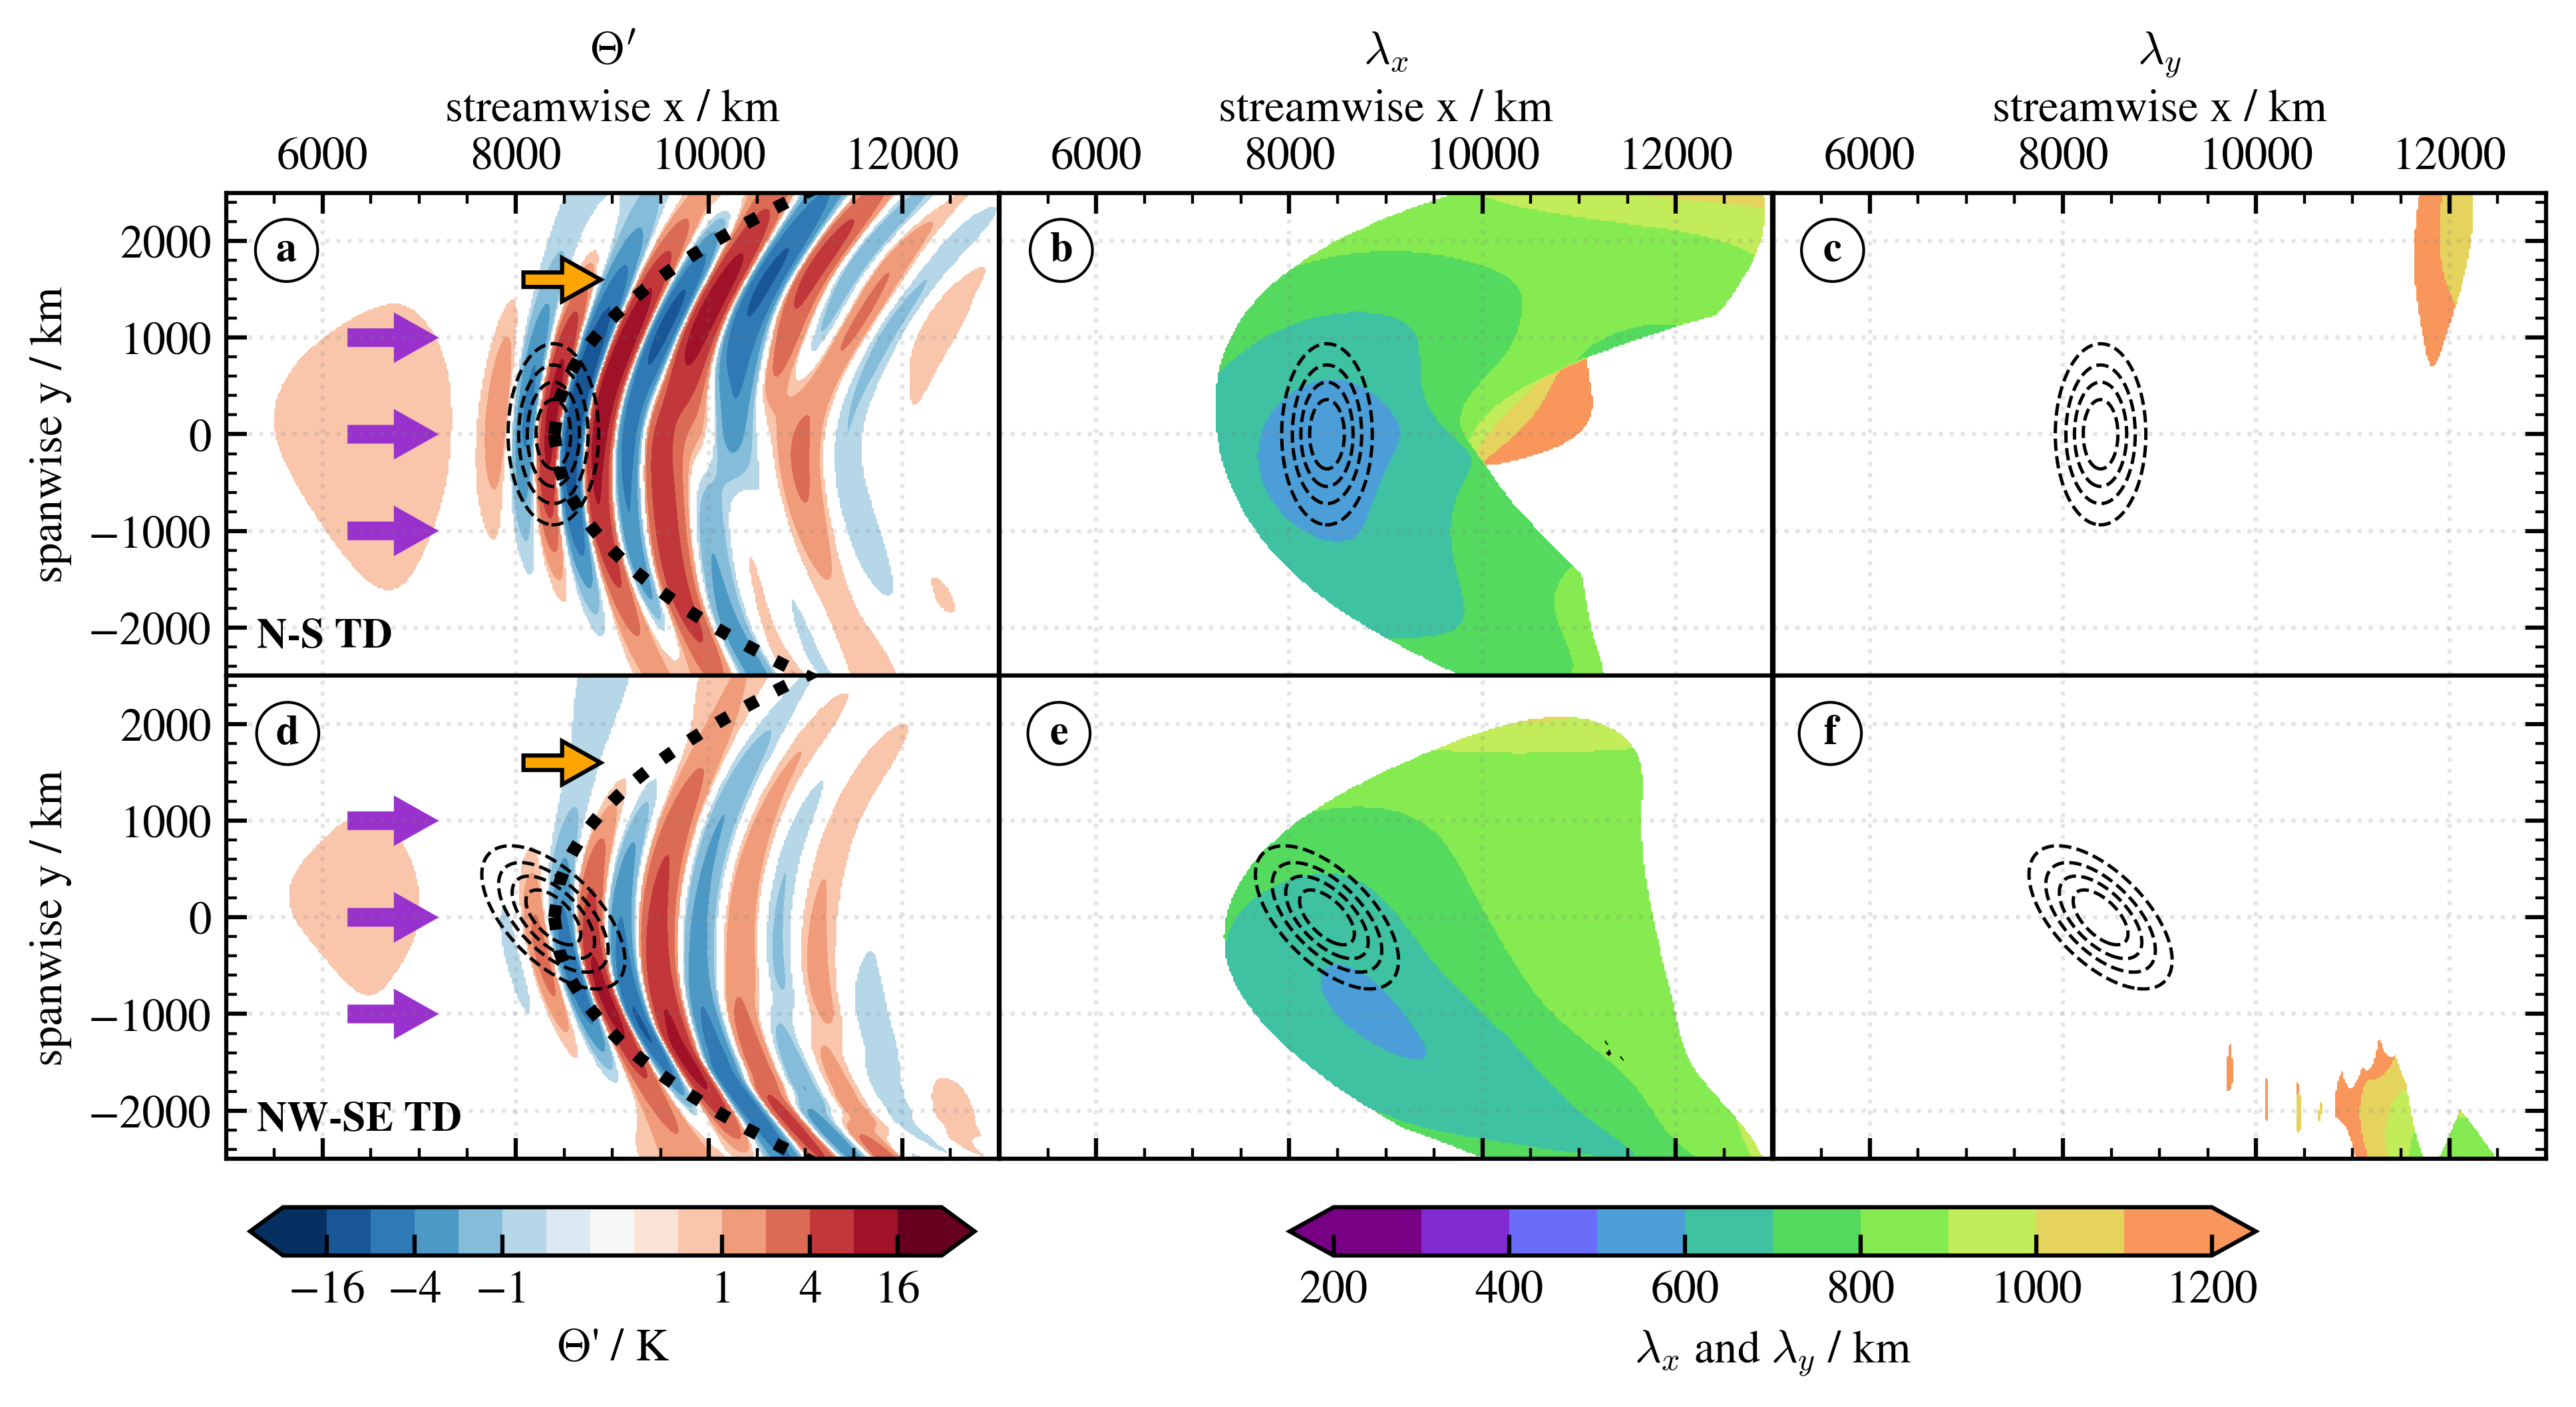
\includegraphics[width=0.99\textwidth]{figures_3D/waveletAna_overview_noShear.png}
    \caption{Horizontal cross sections at 40km above the tropopause for two simulations with no meridional shear as indicated by the purple arrows. Shown are $\Theta$', $\lambda_x$ and $\lambda_y$ after 72h. Dominant wavelengths at each grid point are based on a 1D wavelet analysis in all three dimensions and values below the \SI{95}{\percent} confidence level (with respect to red noise) are left out. The dotted lines in (a) and (d) represent the U-shaped pattern (Equation (\ref{equ:smith_parabola})) of GW activity derived by \textcite[]{smith_linear_1980} for linear MWs above a circular Witch of Agnesi mountain in a non-rotating fluid. The first row (a,b and c) shows a simulation with a tropopause depression oriented north-south, the second row (d,e and f) shows a simulation with a tilted depression.}
    \label{fig:waveletAna_noShear}
    % in a barotropic environment
\end{figure*}
This first section can be seen as a transition from simulations of the previous chapter with no meridional changes to simulations of the remaining chapter with meridional wind shear and meridional variations in the tropopause shape. It discusses two simulations without meridional wind shear, but with an elliptically shaped tropopause depression, so the depth of the tropopause changes spanwise in contrast to simulations of the preceeding chapter. In this way, the effect of the depression's meridional shape on the GW propagation can be isolated and it is not superimposed by the effect of meridional wind gradients.\\
Horizontal cross sections at $z$=\SI{40}{\kilo\meter} and $t$=\SI{72}{\hour} for both simulations are shown in Figure \ref{fig:waveletAna_noShear}. The background wind is similar to the yellow simulation in Figure \ref{fig:q3D_wind} with a $u_{PNJ,max}$=\SI{100}{\meter\per\second} and no meridional gradients as indicated by the purple arrows in (a) and (d). In the upper simulation of Figure \ref{fig:waveletAna_noShear} (a,b and c), the zonal half width of the cosine tropopause depression is again $L_x$=\SI{300}{\kilo\meter} and the meridional one is twice as wide with $L_y$=\SI{600}{\kilo\meter}. In the lower simulation (d,e and f) this tropopause depression is rotated horizontally by \SI{45}{\degree}, so the longer axis of the depression is oriented north-west to south-east (NW-SE). Dashed lines in Figure \ref{fig:waveletAna_noShear} outline the shape of the depression and clarify the orientation. \\
The observed GW pattern in the simulation with a north to south (N-S) oriented depression coincides with the theory of \textcite[]{smith_linear_1980}. The main GW activity aloft mimics a parabola (U-shape) that departs from the center and extends into the lee of the tropopause depression. \textcite[]{smith_linear_1980} neglected rotational effects and derived his linear solutions for GWs above an isolated circular Witch of Agnesi mountain (Equation (\ref{equ:agnesi})) and for a constant wind profile. He states that his results should be applicable to scales from 5 to \SI{50}{\kilo\meter}, but Figure \ref{fig:waveletAna_noShear} demonstrates that it is still a good approximation for variations from the idealized setup and for larger scales that are subject to rotational effects. The thick dotted lines in (a) and (d) represent the solution of Smith's parabola
\begin{equation}
    y^2 = \frac{L \, N}{U} z \, x
    \label{equ:smith_parabola}
\end{equation}
for $L$=\SI{300}{\kilo\meter}, $U$=\SI{100}{\meter\per\second}, $N$=\SI{0.02}{\per\second} and $z$=\SI{40}{\kilo\meter}. The meridional asymmetry of the GW perturbations in (a) is caused by the Coriolis force with slightly stronger perturbations in the north ($f$ of simulations is negative for southern hemisphere), but the general picture in (a) fits to the U-shape described by \textcite[]{smith_linear_1980} for GWs aloft. \\
In the idealized linear setup of \textcite[]{smith_linear_1980} phase lines along the parabola always point back towards the GW source, so the wave's orientation changes proportional to the distance from the source region. In the simulation with a N-S oriented tropopause depression ((a),(b) and (c) in Figure \ref{fig:waveletAna_noShear}) this effect is weak, but noticeable. (b) and (c) depict zonal ($\lambda_x$) and meridional ($\lambda_y$) wavelengths from a 1D wavelet analysis (Section \ref{sec:wavelet}) and, in particular, $\lambda_x$ increases along the parabola and indicates a turning of the horizontal wave-vector. $\lambda_y$ is too large in the proximity of the tropopause fold (besides some values in the top right corner of (c)) and, in this context, phase lines rather point towards a leeward area of the fold and not towards its center, but this discrepancy is plausible and likely results from the elliptic (not circular) shape of the depression.

The effect of tilting the tropopause depression with respect to the zonal flow is apparent in (d),(e) and (f) of Figure \ref{fig:waveletAna_noShear}. A NW-SE oriented depression channels the GW activity southward, though the Coriolis effect counteracts. The shortest wavelenghts are now located south of the depression (bluish colors in (e)) and, again, $\lambda_x$ increases along the parabola while values for $\lambda_y$ are only significant far south-east of the depression in (f). Phase lines along the parabola in (d) tend to point closer to the center of the depression compared to the first simulation in (a), because the difference between the streamwise and spanwise extend of the depression is decreased by the horizontal rotation. \\
Overall, the 3D shape of an obstacle (e.g. a tropopause depression) can influence the propagation direction of the excited GWs and simply rotating the tropopause depression in an environment without meridional wind shear had a significant effect on the GW activity in the upper stratosphere. How this rotation influences the GWs in a realistic scenario with meridional gradients in the background wind will be discussed in Section \ref{sec:3D_shape}. 

% \cite[]{smith_linear_1980}
% $Fr=\frac{U}{h_m \, N} \approx 2$
% shall see that the small-amplitude theory describes the tendency of the flow to be diverted around the mountain but that this theory is valid only for large Froude number F
% All three of the qualitative features; the radial, outward tilting phase lines, the concentration of the disturbance along parabolas which widen with height, and the decay away from the mountain,
% along parabolas which widen with height z, and the decay away from the mountain, are evident 

% The obstacle feels closer to a circular shape for the wind""""
% deflected laterally!
% in the presence of gradients in meridional wind

%%% PNJ with meridional shear %%%
\section{The influence of meridional shear}
\label{sec:3D_shear}
Let us recall the equation for the temporal evolution of the meridional wavenumber from linear ray-tracing
\begin{equation}
    \frac{dl}{dt} = -(k \frac{\partial U}{\partial y} + l \frac{\partial V}{\partial y} + \frac{\beta f}{\hat{\omega}})
    \approx -k \frac{\partial U}{\partial y}
    \label{equ:meridionalRefraction2}
\end{equation}
mentioned in the introduction (e.g. \cite[]{dunkerton_inertiagravity_1984} or \cite[]{eckermann_ray-tracing_1992}). In our simulations $f$ is constant and the background flow is purely zonal, so $\beta=0$ and $\frac{\partial V}{\partial y}=0$ lead to the approximation in Equation (\ref{equ:meridionalRefraction2}). For conservative wave propagation and a stationary background flow $U$, the ground-based frequency $\omega$ is conserved along a ray ($\frac{d \omega}{d t} = 0$) and 
\begin{equation}
    \omega = k c_{P,x} + l c_{P,y} = \textrm{const.}
    \label{equ:const_omega}
\end{equation}
with $c_{P,x}$ and $c_{P,y}$ being the components of the ground-based horizontal phase speed (\cite[]{lighthill_waves_1978} and \cite[]{eckermann_ray-tracing_1992}). Therefore, modifications of $l$ due to the background shear (Equation (\ref{equ:meridionalRefraction2})) always imply a change of $k$ and a turning of the GW. Linear theory also shows that the direction of the horizontal wave vector ($k$,$l$) and of the intrinsic horizontal group velocity are equal for upward propagating GWs (\cite[]{sato_origins_2009}). Under the assumption of a purely zonal background flow the sign of $l$ is equal to that of the ground-based meridional group velocity and represents the direction of wave propagation.\\
The approximation on the right hand side of Equation (\ref{equ:meridionalRefraction2}) shows two terms that are relevant for the generation of a meridional wave component $l$, the meridional shear $\frac{\partial U}{\partial y}$ and the zonal wavenumber $k$. Variations of the zonal wavenumber $k$ or wavelength $\lambda_x$ are closely related to the zonal shape of the tropopause depression and will be discussed in the next section. At first, this section focuses on meridional variations of the background wind.

\begin{figure*}[tbp]
    \centering
    \includegraphics[width=0.99\textwidth]{figures_3D/3D-th-referenceSim.png}
    \caption{The reference simulation of the entirely 3D simulations with meridional background wind shear. (a),(c) and (e) show horizontal cross sections of $\Theta'$ at z=\SI{40}{\kilo\meter} for three timestamps. (b),(d) and (f) show corresponding meridional cross sections \SI{900}{\kilo\meter} in the lee of the propagating tropopause fold. The position is also indicated in the horizontal cross sections by the dashed black lines. The purple lines in (a),(c) and (e) refer to the location of the PNJ. Meridional cross sections also show zonal wind $u$ (dashed lines) and isentropes (solid lines).}
    \label{fig:3D-reference}
\end{figure*}
\begin{figure*}[tbp]
    \centering
    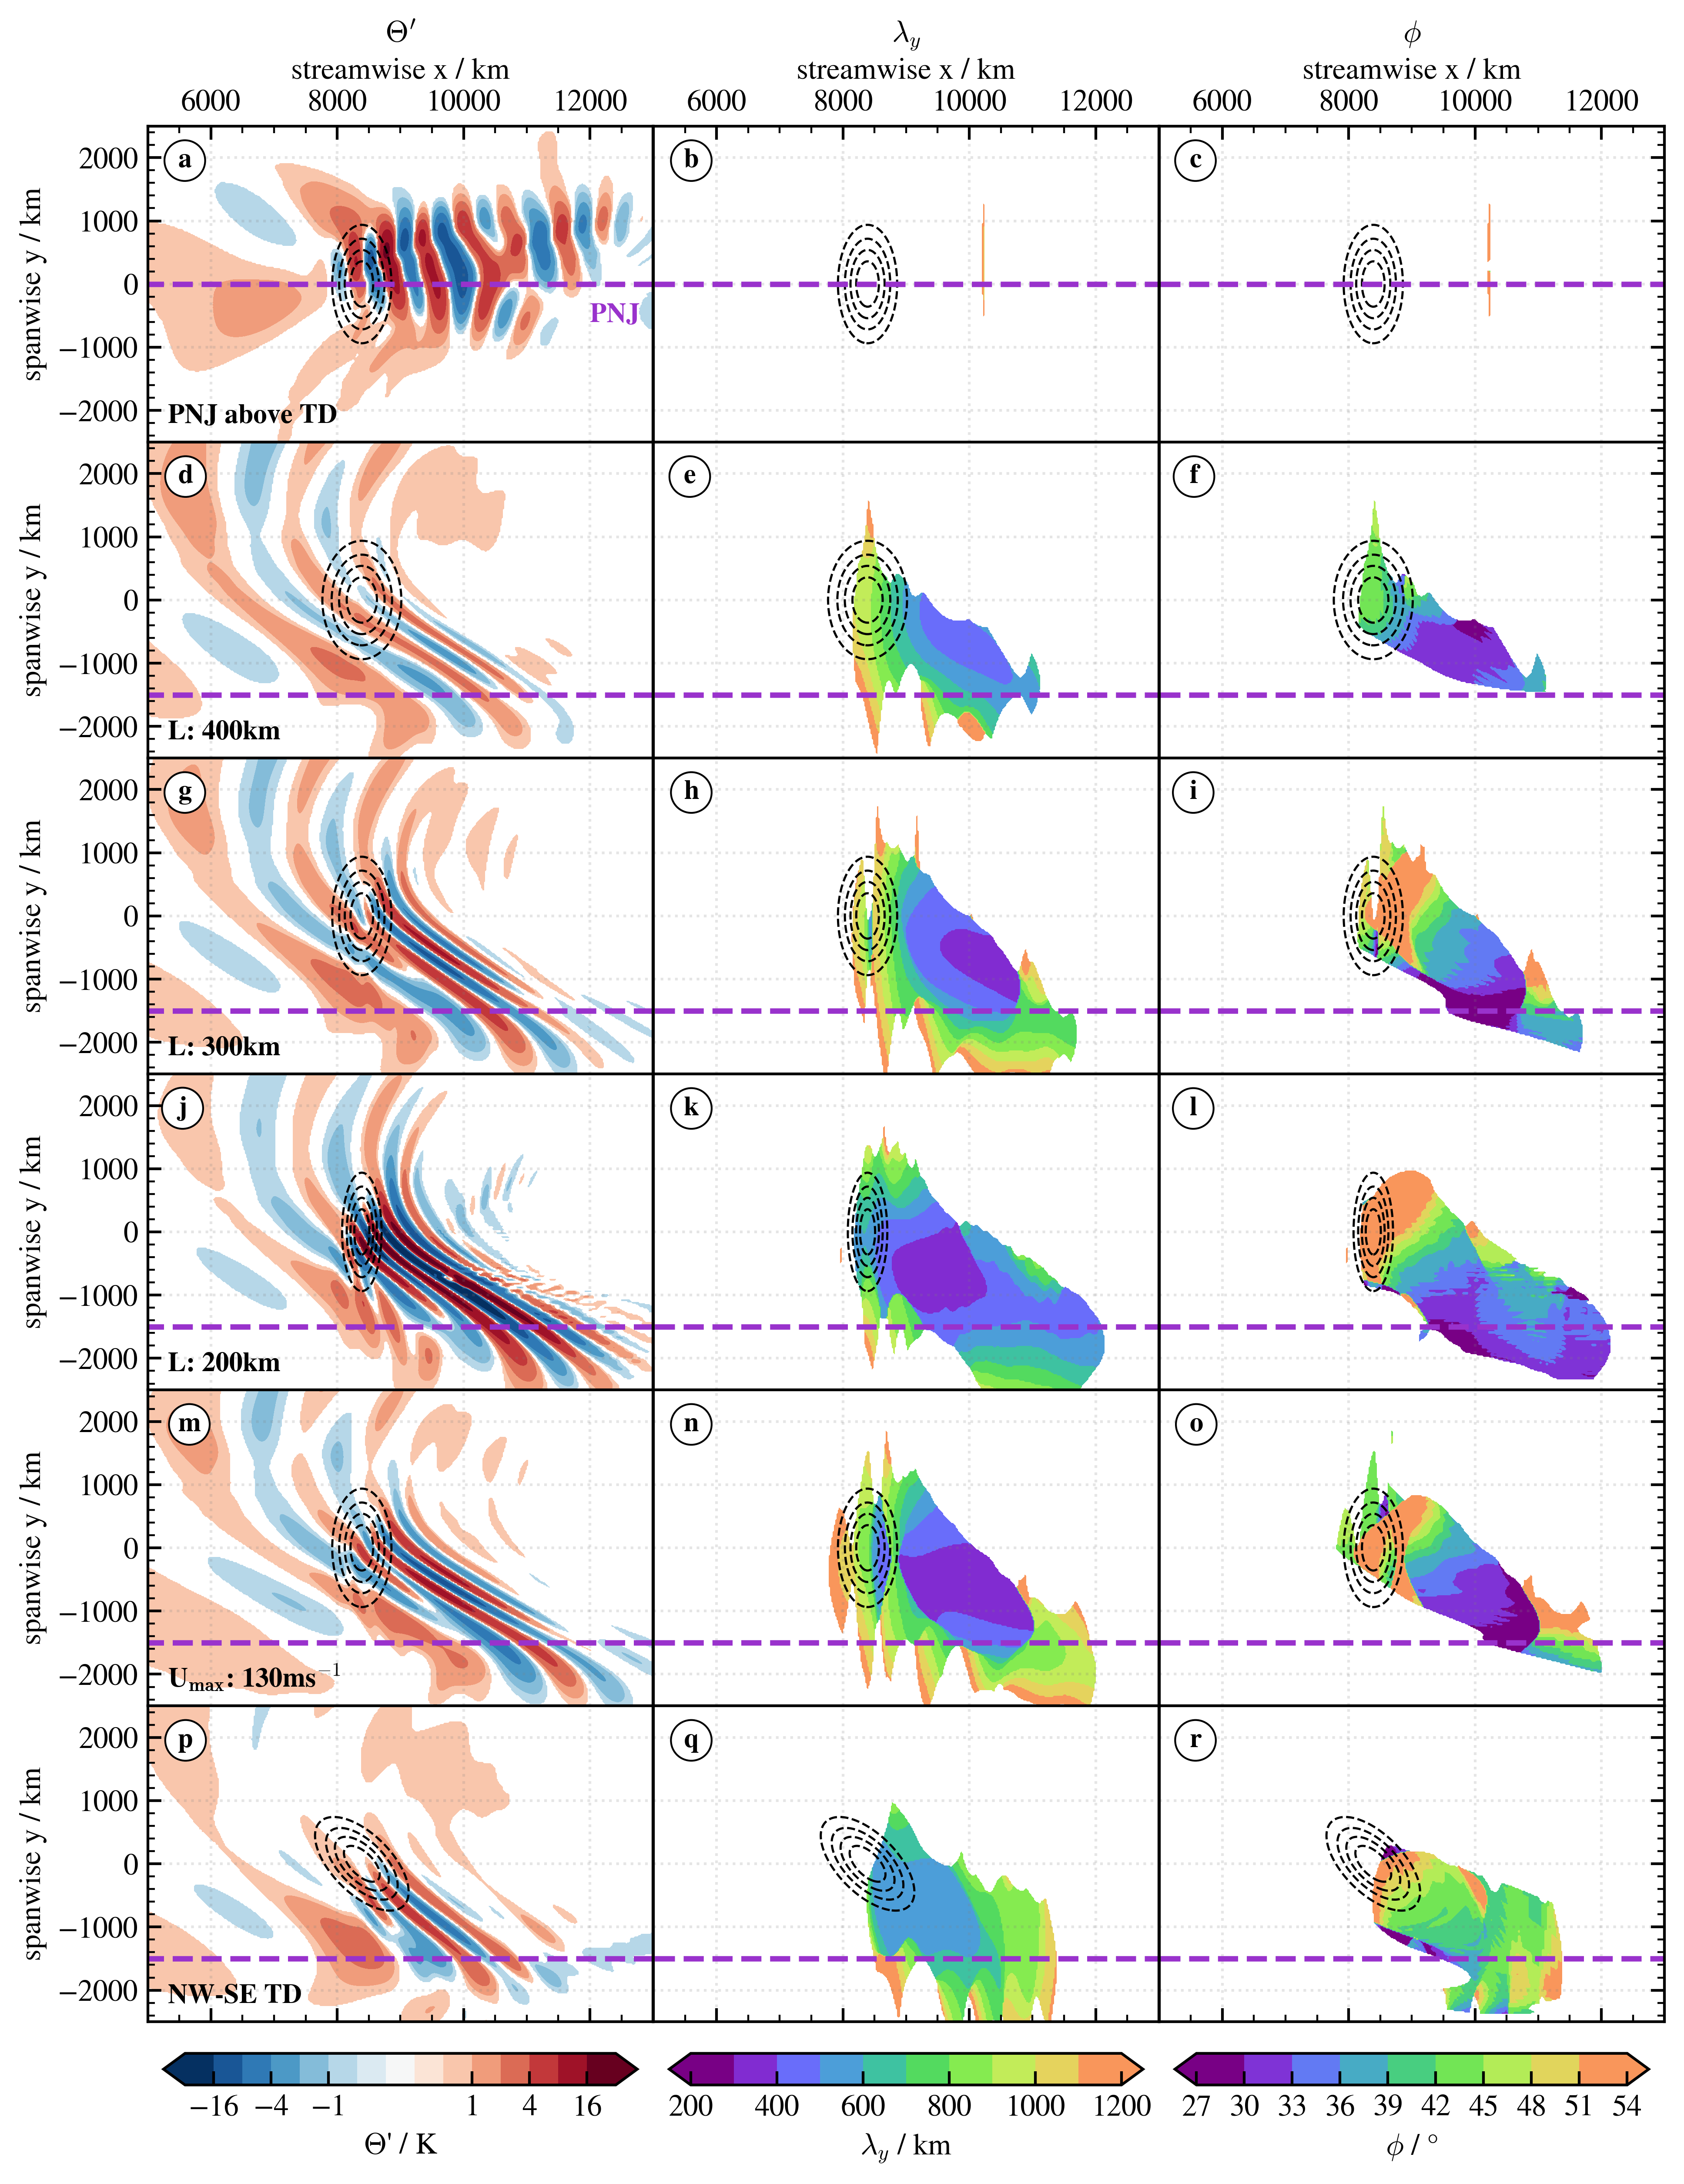
\includegraphics[width=0.96\textwidth]{figures_3D/waveletAna_angle.png}
    \caption{Quite similiar to Figure \ref{fig:waveletAna_noShear}, but showing simulations with meridional wind shear as visualized in Figure \ref{fig:wind_profs}b. Here, $\lambda_y$ moved to the second column and the third column presents the angle $\phi=\arctan(\frac{\lambda_y}{\lambda_x})$ between the phase lines and the x-axis. Again, each row refers to a different simulation and the second and third column is based on a 1D wavelet analysis in each dimension. The corresponding zonal wavelength $\lambda_x$ and the vertical wavelength $\lambda_z$ are plotted in Figure \ref{fig:waveletAna_xz} in Appendix \ref{appA}. The third row ((g),(h) and (i)) is the reference simulation presented in Figure \ref{fig:3D-reference} and labels in each row describe the respective variation. The horizontal purple lines indicate the center of the PNJ.}
    % Hashed areas in the  below \SI{30}{\degree}. For clarification $\phi$ and $\lambda_z$ are plotted in Figure \ref{fig:waveletAna_angle} in Appendix \ref{appA}.
    % Hashed areas in the third column indicate vertical wavelengths larger than \SI{20}{\kilo\meter} at z=\SI{40}{\kilo\meter}.
    \label{fig:waveletAna}
    % between 6 and \SI{20}{\kilo\meter}
\end{figure*}
Figure \ref{fig:3D-reference} and \ref{fig:waveletAna} provide the basis for the following discussion. The first one shows the evolution of the reference simulation for the scenario with meridional wind shear. The center of the PNJ is \SI{1500}{\kilo\meter} south of the tropopause depression centered at $y=0$, because this represents a common scenario above the Southern Ocean west and south of Australia with a PNJ at approximately \SI{60}{\degree S} and Rossby wave trains with tropopause folds further to the north between 30-\SI{55}{\degree S} (\cite[]{skerlak_tropopause_2015}). The 2D wind profile in the meridional cross sections ((b),(d) and (f)) is the product of the vertical wind profile used in the previous section and a meridional distribution centered at $y=\SI{-1500}{\kilo\meter}$ (red curve in Figure \ref{fig:wind_profs}). Similar to the preceding section, the widths of the depression are $(L_x,L_y)=(\SI{300}{\kilo\meter},\SI{600}{\kilo\meter})$ and the tropopause propagates zonally with a constant speed $c_{tf}=\SI{13.88}{\meter\per\second}$. \\
In Figure \ref{fig:3D-reference} GWs excited above the tropopause depression are apparently refracted southward into the PNJ and develop a significant meridional wave-vector component $l$, so phase lines in the horizontal cross sections turn counterclockwise. The wavelet analysis in Figure \ref{fig:waveletAna} confirms this impression. The third row ((g),(h) and (i)) belongs to the reference simulation and, clearly, $\lambda_y$ is smaller south-east of the depression where the GW has propagated into the PNJ. In the same area, the angle $\phi=\arctan(\frac{\lambda_y}{\lambda_x})$ between the phase lines and the x-axis is also smaller and implies a rotation of the wave vector. The corresponding $\lambda_x$ is visualized in Figure \ref{fig:waveletAna_xz} in Appendix \ref{appA} and is larger close to the PNJ. These observations are entirely consistent with linear ray-tracing theory and Equations (\ref{equ:meridionalRefraction2}) and (\ref{equ:const_omega}). MW-like GWs propagate against the background flow and imply a negative $k$. Moreover, the southward shift of the PNJ with respect to the GW source in the center of the domain leads to a negative $\frac{\partial U}{\partial y}$ north of the PNJ and hence $l$ increases in magnitude, but with a negative sign. A negative meridional wave vector component develops and the GW is refracted southward into the PNJ. It is clear that this process is not unlimited. As $l$ increases, $k$ decreases (Equation (\ref{equ:const_omega})) and starts to dampen the further development of a meridional wave component due to $\frac{\partial U}{\partial y}$ in Equation (\ref{equ:meridionalRefraction2}). \\
A PNJ centered above the tropopause depression as in (a),(b) and (c) of Figure \ref{fig:waveletAna} completely alters the GW pattern. Here, $\frac{\partial U}{\partial y}$ is negative in the north of the depression and positive in the south. GWs that propagate to the north (south) develop a negative (positive) $l$ and are refracted back towards the center of the domain. Again, GWs propagate towards the maximum wind speed of the PNJ, but in this scenario the generation of a meridional wave component $l$ is suppressed and phase lines stay more or less orthogonal to the zonal backgroud flow. \\ % as depicted in (a) and (b) of Figure \ref{fig:waveletAna}
In the simulation of (m),(n) and (o) (row five of Figure \ref{fig:waveletAna}) the maximum wind speed of the PNJ is increased from $U_{PNJ,max}=\SI{100}{\meter\per\second}$ to $U_{PNJ,max}=\SI{130}{\meter\per\second}$. Signs for $k$ and $\frac{\partial U}{\partial y}$ are similar to the reference simulation, so GWs also propagate southward. However, the development of a negative $l$ and the corresponding turning of the wave is stronger, because the absolute value of $\frac{\partial U}{\partial y}$ is larger. Comparing (h) and (i) to (n) and (o) in Figure \ref{fig:waveletAna} supports this statement. $\lambda_y$ in (n) is generally smaller than in (h) and $\phi$ in (o) indicates a trend towards more horizontal phase lines with smaller $\lambda_y$ (wide purple area north of the PNJ), too.\\
We note that GW phase lines in the horizontal cross section at z=\SI{40}{\kilo\meter} (Figure \ref{fig:waveletAna}m) appear quite similar to the zonally elongated phase lines in the ERA5 data (Figure \ref{fig:RF25_era5_horizonal}) observed by \textcite[]{dornbrack_stratospheric_2022} and addressed in research question (R1). Strong winds in the upper stratosphere and the southward position of the PNJ seem to be crucial, if not necessary, features to observe such a GW pattern. Either way, these conditions are likely in the southern hemisphere and propagating tropopause depressions potentially excite those GWs with zonally elongated phase lines. The influence of the tropopause shape in the presence of meridional wind shear is discussed in the next section.

% Another view on this refraction of GWs into the PNJ are critical levels... ??
% ground-based horizontal phase speed is always parallel to K 
% This lies the foundation for the following discussion.
% relative to the mean wind = intrinsic
% A = E/\omega$ = const.$  is the wave action 
% $ \omega = \hat{\omega} + k U = const.$ 
% beta = df/dy so beta plane approximation, usually also gradient of f changes on Earth
% trailing GWs 

\section{The influence of the tropopause shape in the context of meridional shear}
\label{sec:3D_shape}
%As stated in the previous section, 
The zonal wavenumber $k$ in Equation (\ref{equ:meridionalRefraction2}) is closely linked to the zonal width of the tropopause depression. A depression with a smaller width excites GWs with a smaller horizontal scale (larger $k$) and consequently, the growth of a meridional wave component $\frac{dl}{dt}$ in the presence of meridional wind shear is greater. The second (fourth) row of Figure \ref{fig:waveletAna} displays a simulation with a wider (narrower) tropopause depression as the reference simulation. Comparing these three simulations confirms the ray-tracing theory. The smaller the depression's zonal width, the smaller $\lambda_x$ ((e),(h) and (k) in Figure \ref{fig:waveletAna_xz}) and the smaller $\lambda_y$ ((f),(i) and (l)in Figure \ref{fig:waveletAna}) in the upper stratosphere. In Chapter \ref{sec:resultsQ3D}, we also concluded that the GW activity in the stratosphere is inversely proportional to the width of the tropopause depression. Figure \ref{fig:waveletAna_mf} in Appendix \ref{appA} further substantiates this fact and emphasizes that the zonal ((e),(h) and (k)) and the meridional ((f),(i) and (l)) momentum flux increases for smaller depression widths. \\
A decreasing depression width implies decreasing GW scales and an increase in the meridional momentum flux, but does it also influence the orientation of the wave vector? In this context, we again refer to the angle $\phi$ at $z=\SI{40}{\kilo\meter}$ in the third column of Figure \ref{fig:waveletAna}. Though variations of the depression width are high between simulations, there is no clear trend of the ratio $\frac{\lambda_y}{\lambda_x}$ or the orientation of the wave vector ((f),(i) and (l)). All three simulations exhibit a similar pattern with rather spanwise oriented phase lines above and in the lee of the depression, and more streamwise oriented phase lines closer to the PNJ where the $\frac{\partial U}{\partial y}$ increases. But a trend towards smaller $\phi$, as for the stronger PNJ in row 5 of Figure \ref{fig:waveletAna}, is not observable.

\begin{figure*}[t]
    \centering
    \includegraphics[width=0.99\textwidth]{figures_3D/3D-EF-MF.png}
    \caption{Similar cross sections as Figure \ref{fig:3D-reference} with horizontal cross sections at z=\SI{40}{\kilo\meter} in (a) and (c) and meridional cross sections in (b) and (d) for x=\SI{9400}{\kilo\meter} showing meridional momentum flux MF$_y$ instead of $\Theta'$. The first row is again the 3D "reference" simulation at $t=\SI{72}{\hour}$, the second row is a simulation with identical settings, but a NW-SE oriented tropopause depression. In other words, the depression is rotated horizontally by 45°. Black arrows in (a) and (c) illustrate the direction and relative value of the horizontal energy flux \textbf{EF}. The reference simulation is the third row and the simulation with a rotated depression is represented by the last row in Figure \ref{fig:waveletAna}.}
    \label{fig:3D-MFy}
\end{figure*}
The last row in Figure \ref{fig:waveletAna} presents a simulation with a rotated tropopause depression as in Section \ref{sec:3D_noshear}, but in the presence of meridional wind shear. Interestingly, $\lambda_y$ and $\phi$ are larger for the NW-SE oriented depression, so tilting the depression counteracts the development of $l$ and zonally elongated phase lines. It seems counterintuitiv, because the orientation of the depression already leads to a small meridional wave vector component in the no-shear case of Section \ref{sec:3D_noshear}. However, the wider width in the direction of the background flow reduces $k$ and the growth of $l$ and, therefore, constrains the refraction and meridional propagation of the GW. Figur \ref{fig:3D-MFy} further illustrates this fact. The meridional momentum flux MF$_y$ is lower for the simulation with a tilted depression in the horizontal cross section (c) and the meridional cross section (d) compared to (a) and (b) for a N-S oriented depression with an identical size. Vectors of the energy flux \textbf{EF} in (a) and (c) clarify the southward propagation of the GWs into the PNJ and the intrinsic propagation against the prevailing wind for both simulations, but, again, \textbf{EF} is slightly greater for the N-S oriented depression.

Overall, the meridional momentum and energy fluxes significantly increase for smaller zonal widths of the tropopause depression, but $\phi$ or the zonally elongated phase line pattern in the upper stratosphere is not directly sensitive to the depression's zonal width, only to its orientation. A NW-SE oriented depression does not favour elongated phase lines (small $\phi$), because its width in the direction of the background flow increases.

% general statement on momentum fluxes larger for smaller scale GWs

\section{Momentum flux calculation from an observational perspective}
\label{sec:3D_mf}
In numerical simulations the vertical flux of horizontal momentum (MF) can be calculated directly from available wind perturbations ($u'$,$v'$ and $w'$) by utilizing equation \ref{equ:mf}. It was used in the preceding sections, too. However, most satellite or ground-based instruments that provide observations of the stratosphere and MLT on a reasonable scale to study GWs are only capable of measuring temperature (e.g. \cite{wu_satellite_1996}, \cite[]{ern_absolute_2004}, \cite{hindley_gravity_2019}, \cite{kaifler_compact_2021}). Temperature perturbations alone allow the calculation of potential energy distributions, but usually momentum flux is the variable of interest to investigate wave-mean flow interactions in the middle atmosphere and constrain GW parameterizations in climate simulations (\cite[]{geller_comparison_2013} or \cite[]{kim_overview_2003}). \\
In this context, \textcite[]{ern_absolute_2004} derived a formulation of MF that depends on the temperature amplitude $\hat{T}$ and the wave's horizontal and vertical wavelength instead of $\overbar{u'w'}$. They start with the expression of the vertical flux of horizontal pseudomomentum valid for conservative wave propagation
\begin{equation}
    (\mathrm{MF}_x, \mathrm{MF}_y) = \bar{\rho} (1-\frac{f^2}{\hat{w}^2}) \Bigl(\overbar{u'w'},\overbar{v'w'}\Bigr) 
    % \approx \bar{\rho}  (\overbar{u'w'},\overbar{v'w'})
    \label{equ:ps-mf}
\end{equation}
(\cite[]{fritts_gravity_2003}). We follow their convention and refer to it as momentum flux MF with MF$_x$ and MF$_y$ being the zonal and meridional MF respectively. They utilize the generally valid linear polarization relations (Equation (14) in \textcite[]{fritts_gravity_2003}) and the dispersion relation
\begin{equation}
    \hat{w}^2 = \frac{N^2 \Bigl(k^2+l^2\Bigr) + f^2 \Bigl(m^2 + \frac{1}{4H^2}\Bigr)}{k^2+l^2+m^2+\frac{1}{4H^2}}
    \label{equ_lid:dispersion_noAss}
\end{equation}
from \textcite[]{fritts_gravity_2003} to end up with
\begin{equation}
    (\mathrm{MF}_x, \mathrm{MF}_y) = A \cdot B \frac{\bar{\rho}}{2} \Bigl(\frac{g}{N}\Bigr)^2 {\Bigl(\frac{\hat{T}}{\bar{T}}\Bigr)^2} \Bigl(\frac{k}{m},\frac{l}{m}\Bigr).
    \label{equ:mf-tp}
\end{equation}
The only assumptions that accompany equation \ref{equ:mf-tp} are a monochromatic wave perturbation and hydrostatic equilibrium. In \textcite[]{ern_absolute_2004} and many follow-up publications (e.g. \cite[]{preusse_characteristics_2014}, \cite[]{ern_gracile_2018}, \cite[]{hindley_gravity_2019}) the factors $A$ and $B$ are neglected by refererring to the midfrequency approximation. NOGWs above tropopause depression can be considered low frequency waves with large horizontal wavelengths. It needs to be checked if $A$ and $B$ are still neglible in this spectral range. While the factor
\begin{equation}
    \begin{split}
        A = &\biggl(1-\frac{\hat{\omega}^2}{N^2}\biggr) \biggl(1 + \frac{1}{m^2} \Bigl(\frac{1}{2H}-\frac{g}{c_s^2}\Bigr)^2\biggr)^{-1} \\
            &\biggl(1+\Bigl(\frac{f}{m \hat{\omega}}\Bigr)^2 \Bigl(\frac{1}{2H} - \frac{g}{c_s^2}\Bigr)^2\biggr)^{0.5}
    \end{split}
    \label{equ:A}
\end{equation}
naturally appears following the approach of \textcite[]{ern_absolute_2004}. The factor
\begin{equation}
    B = \left| \frac{\tilde{\Theta}}{\tilde{T}} \right|^2 = \left| 1 + \frac{1}{\beta} \frac{\gamma-1}{c_s^2} \frac{\hat{\omega}}{\frac{N^2}{g}}i\right|^{-2}
    \label{equ:B}
\end{equation}
with
\begin{equation}
    \beta = -\frac{\hat{\omega}}{N^2-\hat{\omega}^2} \biggl(m + \Bigl(\frac{1}{2H}-\frac{g}{c_s^2}\Bigr)i\biggr)
    \label{equ:beta}
\end{equation}
represents the error by assuming equal amplitudes for $\hat{\Theta}$ and $\hat{T}$ considering all motions to be adiabatic (\cite[]{fritts_gravity_2003} and \cite[]{ern_directional_2017}).
\begin{wrapfigure}{r}{7.5cm}
    \includegraphics[width=7.5cm]{figures_3D/waveletAna_mfcorrection_factor.png}
    \caption{The correction factor A$\cdot$B in equation \ref{equ:mf-tp} for a range of vertical and horizontal wavelengths. It is reproduced from \textcite[]{ern_directional_2017} (supporting information) for a larger $f$ and smaller $c_s$. The dashed rectangle contains all combinations of wavelenghts from the wavelet analysis.}
    \label{fig:mf_correction}
\end{wrapfigure}
In their supporting information \textcite[]{ern_directional_2017} visualize $A$ and $B$ for a common range of vertical and horizontal wavelengths and typical stratospheric values of $N=\SI{0.02}{\per\second}$, $H=\SI{7}{\kilo\meter}$ and $T=\SI{250}{K}$ resulting in $c_s = \SI{316}{\meter\per\second}$. Furthermore, $\gamma=0.4$ and $g=\SI{9.81}{\meter\per\second^2}$. The Coriolis parameter $f$ was chosen for a latitude of 30°. All values are representative for the idealized simulations of this work, but $f$ was a factor of 1.64 larger in the simulations and the background temperature of the isothermal atmosphere was $T=\SI{239}{K}$. Therefore, Figure (S1c) of \textcite[]{ern_directional_2017} is reproduced in Figure \ref{fig:mf_correction} for a Coriolis parameter $f=\SI{1.2e-4}{\per\second}$ (latitude of 55°) and $c_s = \SI{310}{\meter\per\second}$ due to $T=\SI{239}{K}$. \\
Adapting the Coriolis parameter had no noticeable effect. Lowering $c_s$ made $A \cdot B$ smaller, so less negligible, but the factor is still greater than $0.95$ for most combinations of wavelengths appearing in the simulations (dashed rectangle). In general, Figure \ref{fig:mf_correction} clarifies that $A \cdot B$ is much more significant for non-hydrostatic or high frequency waves, while GWs with large horizontal scales are less affected and $A \cdot B$ can be neglected for the following comparison.

At this point, it is important to clarify another relation. \textcite[]{ern_absolute_2004} derived an equation for the momentum flux that depends on the wave's temperature amplitude $\hat{T}$. $\hat{T}$ results from the spectral analysis of the 3D temperature measurements just like horizontal and vertical wavelengths and refers to the amplitude of a perfect sine or cosine wave. These spectral analysis methods improved consistently over the past two decades. Examples are the "S3D" method by \textcite[]{lehmann_consistency_2012} or the work of \textcite[]{wright_exploring_2017} who extended the Stockwell transform to 3D and applied it to new satellite measurements with AIRS (see also \cite[]{hindley_gravity_2019} and \cite[]{hindley_18year_2020}). When following these analysis methods it makes sense to use $\hat{T}$ for calculating MF, because maximum amplitudes might be missed by the coarse resolution of the measurements. In contrast, numerical models provide temperature perturbations $T'$ on a regular grid and it is possible to calculate MF directly via the temperature variance $\overbar{T'^2}$. Again, the overbar denotes averaging over one or multiple full wave cycles. Relating $\overbar{T'^2}$ to $\hat{T}^2$ yields
\begin{equation}
    \overbar{T'^2} = \overbar{\hat{T} sin(\phi)^2} = \frac{1}{2}\hat{T}^2,
    \label{equ:tvariance}
\end{equation}
because $\overbar{sin(\phi)^2} = \frac{1}{2}$. Since temperature variance defines the eddy potential energy per unit mass $E_p$ (first row in equation \ref{equ:epot}), we can use equation \ref{equ:tvariance} to rewrite $E_p$ in terms of $\hat{T}$
\begin{equation}
    \begin{split}
        E_p &= \frac{1}{2} \Bigl(\frac{g}{N}\Bigr)^2 \overbar{\Bigl(\frac{T'}{\bar{T}}\Bigr)^2} \\
            &= \frac{1}{4} \Bigl(\frac{g}{N}\Bigr)^2 \Bigl(\frac{\hat{T}}{\bar{T}}\Bigr)^2
    \end{split}
    \label{equ:epot}
\end{equation}
and relate it to the momentum flux
\begin{equation}
    (\mathrm{MF}_x, MF_y) = \bar{\rho} \Bigl(\frac{g}{N}\Bigr)^2 \overbar{\Bigl(\frac{T'}{\bar{T}}\Bigr)^2} \Bigl(\frac{k}{m},\frac{l}{m}\Bigr) = 2 \bar{\rho} E_p \Bigl(\frac{k}{m},\frac{l}{m}\Bigr)
    \label{equ:mf-epot}
\end{equation}
based on equation \ref{equ:mf-tp} and neglecting the factor $A \cdot B$ (\cite[]{ern_gracile_2018}, \cite*[]{ern_intermittency_2022}). From Figure \ref{fig:mf_correction} it is clear that the factor $A \cdot B$ is neglible for the low frequency GWs excited above tropopause folds, so in the following  we will use equation \ref{equ:mf-epot} to calculate the pseudomomentum flux from temperature perturbations. In a similar manner it is possible to show that the factor $\bigl(1-\frac{f^2}{\hat{\omega}^2}\bigr)$ in equation \ref{equ:ps-mf} can be neglected to calculate the pseudomomentum flux from wind perturbations. Again, the factor is greater than 0.95 for most combinations of horizontal and vertical wavelengths that appear in the idealized simulations, so the vertical flux of horizontal pseudomomentum is underestimated by about \SI{5}{\percent} or less when replaced by the conventional momentum flux $\bar{\rho}(\overbar{u'w'},\overbar{v'w'})$ (equation \ref{equ:mf}) under the midfrequency approximation ($N >> \hat{\omega} >> f$). \\
For a broader understanding we can obtain another perspective on this error by introducing the total energy
\begin{equation}
    E_0 = E_k + E_p = \frac{1}{2} \Bigl(\overbar{u'^2} + \overbar{v'^2} + \overbar{w'^2}\Bigr) + \frac{1}{2} \Bigl(\frac{g}{N}\Bigr)^2 \overbar{\Bigl(\frac{T'}{\bar{T}}\Bigr)^2}
    \label{equ:etot}
\end{equation}
with the kinetic energy per unit mass $E_k$ (e.g. \cite[]{gill_atmosphere-ocean_1982} or \cite[]{tsuda_global_2000}). For non-rotating GWs the kinetic and potential energy tend to be the same ($ E_k \approx E_p$). In that case, the wave energy is equipartiioned and from equation \ref{equ:mf-epot} it follows
\begin{equation}
    \mathbf{MF} = 2 \bar{\rho} E_p \frac{\mathbf{K}}{m} = \bar{\rho} E_{0} \frac{\mathbf{K}}{m}
    \label{equ:mf-etot}
\end{equation}
with the horizontal wavenumber vector $\mathbf{K}$ (compare to \cite[]{andrews_wave-action_1978} or \cite[]{fritts_gravity_2003}). The kinetic energy part becomes more and more dominant for low frequency waves (\cite[]{gill_atmosphere-ocean_1982}), so the error of calculating the pseudomomentum flux under the midfrequency approximation (equation \ref{equ:mf} and \ref{equ:mf-epot}) is proportional to $\frac{E_k}{E_p}$.  

After this extensive discussion on relevant approximations and relations, Figure \ref{fig:mf_scatter} finally compares zonal and meridional MF from wind perturbations to MF from temperature perturbations for all 3D simulations in Figure \ref{fig:waveletAna}.
\begin{figure*}[t]
    \centering
    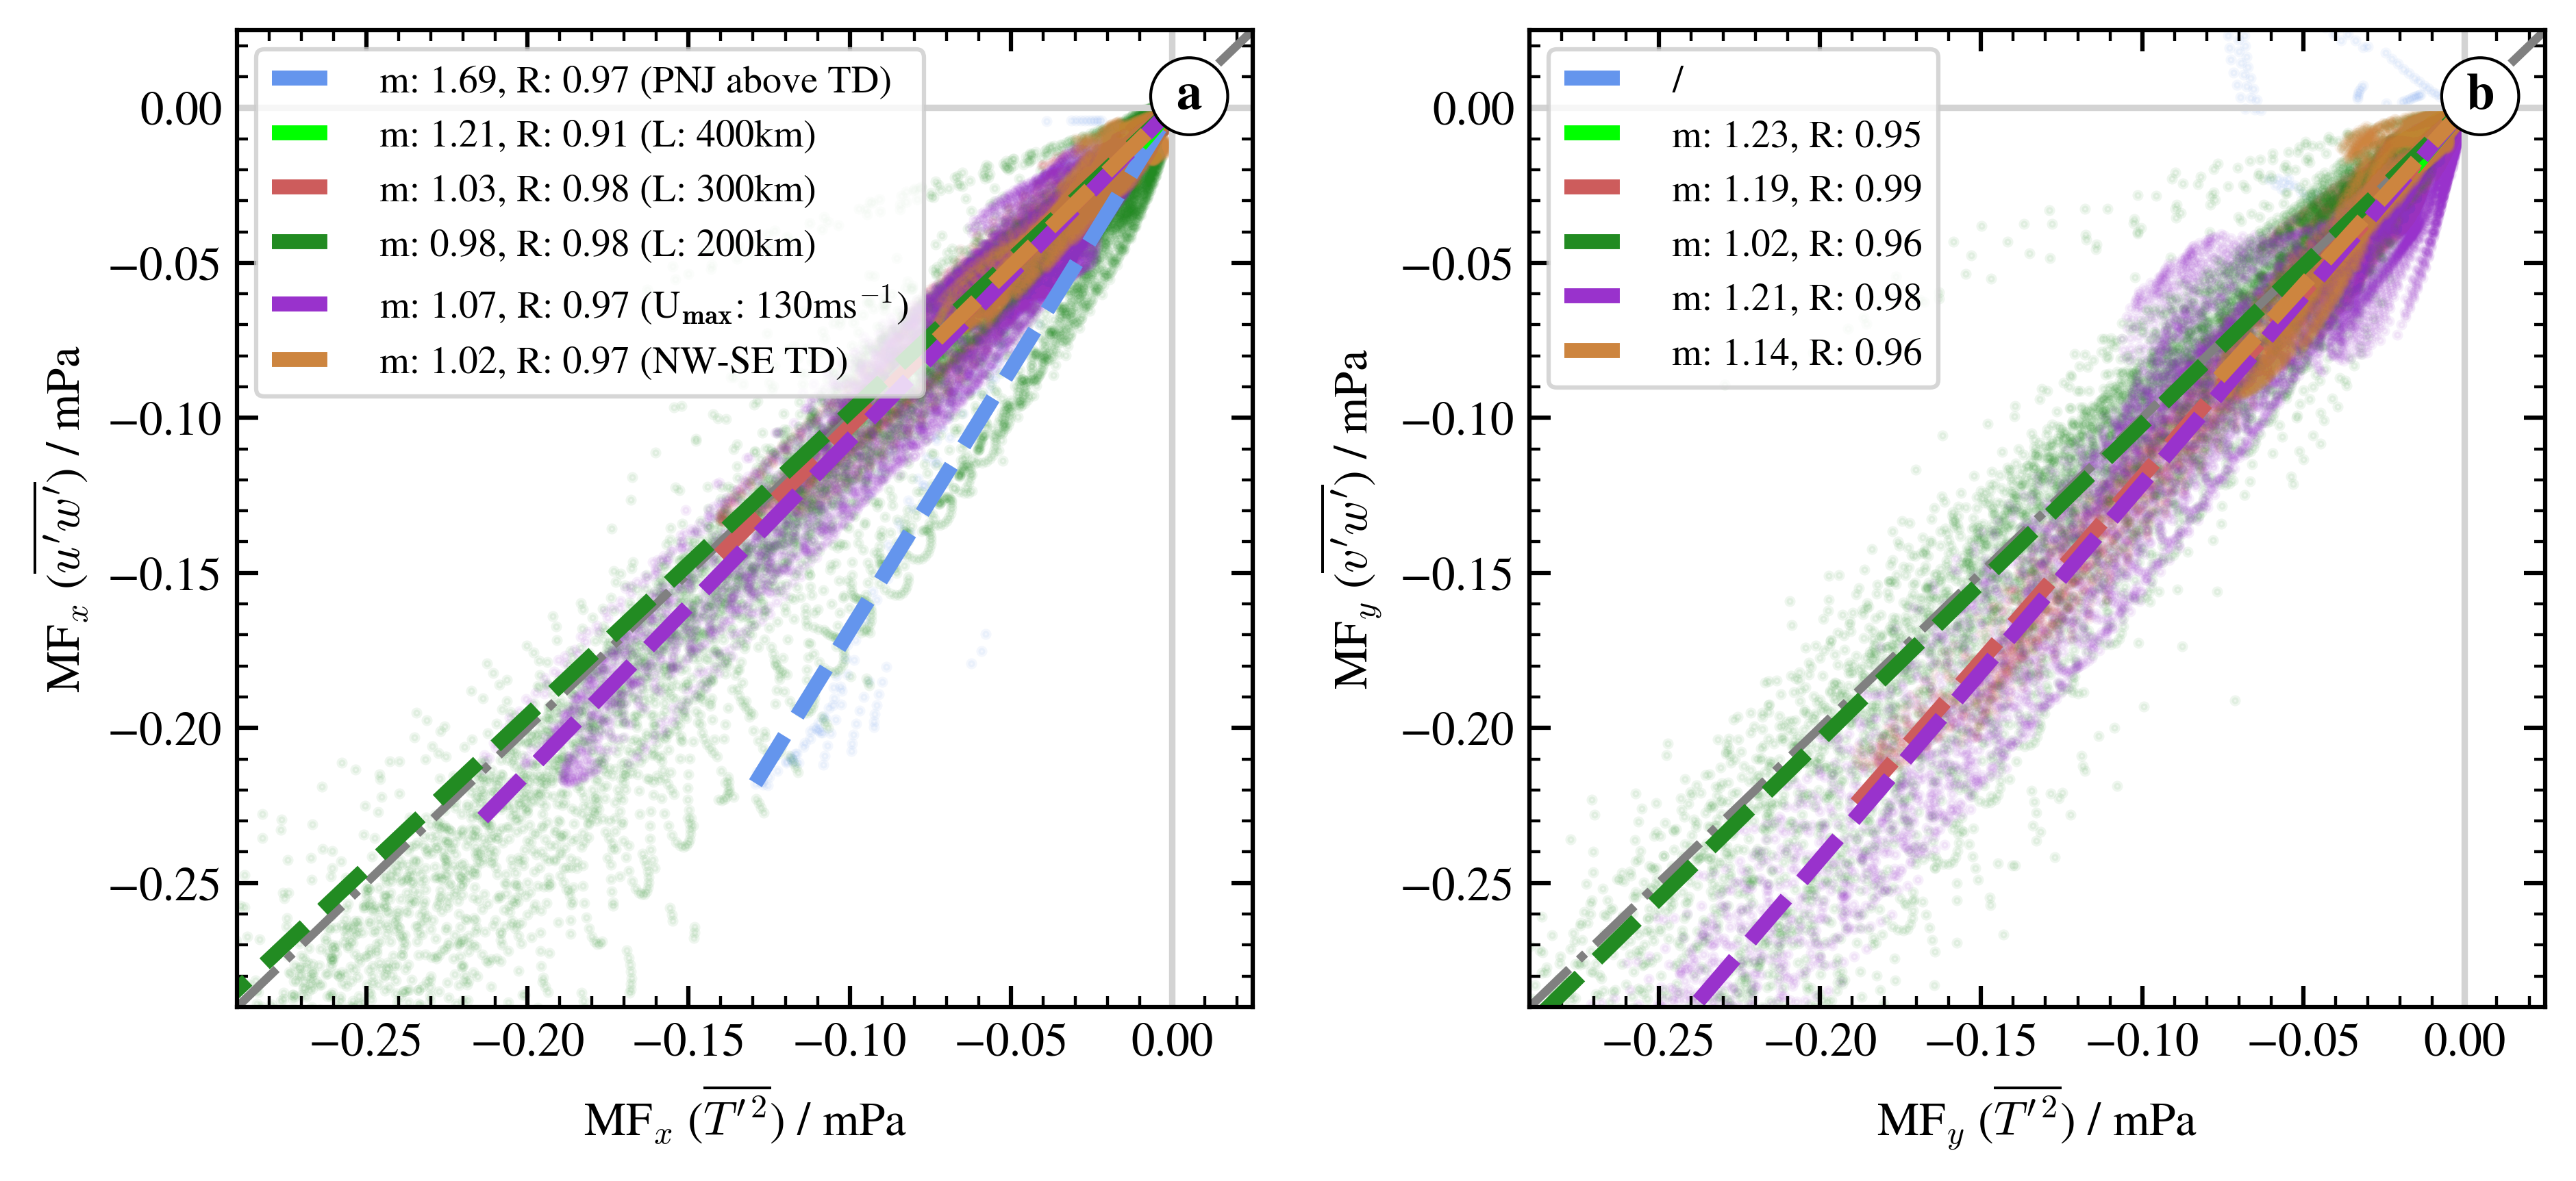
\includegraphics[width=0.99\textwidth]{figures_3D/waveletAna_mf_scatter.png}
    \caption{Scatter plots of the zonal (a) and meridional (b) MF at z=\SI{40}{\kilo\meter} after 72h for all simulations in Figure \ref{fig:waveletAna}. The x-axis refers to the MF calculated from temperature perturbations, the y-axis refers to the MF calculated from wind perturbations. Colored dashed lines are linear fits with slope m and intercept $y_{0}=0$ for each individual simulation.}
    \label{fig:mf_scatter}
\end{figure*}
Overall, momentum fluxes from wind and temperature correlate well. R values are high for all simulations, so linear regressions in Figure \ref{fig:mf_scatter} represent meaningful relations. Especially linear fits of the zonal MF show a good agreement with slope values $m \approx 1$ with one exception. For reasons not fully understood, the slope of the linear regression for the simulation with the PNJ centered above the propagating tropopause depression has a slope of $m \approx 1.7$. In this simulation setup GWs propagate upward into the PNJ without a turning of phase lines resulting in no meridional flux. Nevertheless, we would expect the correlation of the MF$_x$ to be similar to the remaining simulations. \\
MF$_y$ (Figure \ref{fig:mf_scatter}b) also shows good agreement, but a general low bias of temperature-based with respect to wind-based MF can be observed. Only the simulation for the smallest depression width $L=\SI{200}{\kilo\meter}$ has an almost perfect slope while the general picture indicates $15-\SI{25}{\percent}$ higher values for MF$_y$ from winds.\\
MF$_x$ and MF$_y$ suggest a higher correlation for smaller depression widths $L$. Three simulations ($L=400,300,\SI{200}{\kilo\meter}$) are not enough to be conclusive here, but this trend could be related to the effect of rotation that becomes more relevant for wider tropopause folds that result in larger horizontal wavelengths and lower intrinsic frequencies $\hat{\omega}$. As discussed in the beginning of this section, the neglected factor $A \cdot B$ for the MF from $T'$ is not sensitive to large horizontal scales or an increased impact of Coriolis. On the other hand, the factor $\bigl(1-\frac{f^2}{\hat{\omega}^2}\bigr)$ in equation \ref{equ:ps-mf} decreases for smaller $\hat{\omega}$, so MF from wind is overestimated, when this factor is neglected for low frequency waves with $\hat{\omega}$ approaching $f$. Maybe it is this simplification under the midfrequency approximation that becomes less valid and leads to a higher MF from winds for wider tropopause folds.

Despite these uncertainties, we conclude that the calculation of MF from temperature perturbations still leads to meaningful results for the spectrum of GWs excited by propagating tropopause depressions. Considering the uncertainty of real measurements the correspondence between temperature-based and wind-based MF is very good and uncertainties due to the calculation are tolerable. In addition, it shows that the majority of the GWs within the idealized simulations obey the polarization and dispersion relations of GWs and propagate linearly up to an altitude of at least \SI{40}{\kilo\meter}. The analysis of horizontal cross sections at lower levels leads to similar conclusions and is therefore left out.

% zero intercept was used, so larger fluxes might have stronger influence slope value??
% A particularly striking result is a widespread 

% The right part in equation \ref{equ:mf-etot} fits to the work of \textcite[]{andrews_wave-action_1978} or the work of \textcite[]{fritts_spectral_1993} who derived energy spectra in the upper atmosphere from observations. 

% Vertical timeseries of temperature from Lidar observations usually aren't sufficient to derive horizontal momentum fluxes without additional information or assumptions for horizontal wavelengths.
% Gracile paper (Ern 2018) states a factor of Ekin/Epot = 5/3???? should be E0/Epot??
% $f$ is the inertial frequency
% p=5/3 (intrinsic frequency ωˆ spectrum of the GW wave energy density assumed to decrease with ωˆ−5/3)
% The acceleration or deceleration (X, Y ) of the background flow, in the following for simplification called gravity wave drag, is given by the vertical gradient of momentum flux: (X, Y ) = − 1 % ∂ (Fpx, Fpy ) ∂z , (12) with X and Y the drag in the zonal and meridional directions, respectively, and z the vertical coordinate.
 
% F = rho * k/m * Epot,max.
% Es gilt also Etot = Ekin + Epot = Epot,max (in Worten... zum Zeitpunkt, wo die potentielle Energie über die Schwingung maximal wird verschwindet der kinetische Anteil --> Ekin = 0). Wenn wir nun F allein aus den Temperaturvarianzen berechnen wollen nehmen wir an, dass
% Epot {gemittelt über eine Wellenperiode} = Ekin {gemittelt über eine Wellenperiode} (hier kommen dann wohl Annahmen wie linear und non-dissipative mit rein). Daraus folgt dann 
% --> Etot = 2 * Epot {gemittelt über eine Wellenperiode}
% --> F = rho * k/m * 2*Epot {gemittelt über eine Wellenperiode} = rho * k/m *(g/N)^2 * average((T'/T)^2)

\section{Summary and answer to research question (R2) and (R3)}
\label{sec:3D_summary}
This chapter mainly presented 3D simulations of the stratosphere with identical resolutions in streamwise and spanwise direction, with meridional gradients of the lower boundary (tropopause) and with vertical and meridional gradients in the zonal background flow. It is the most realistic setup within the framework of this thesis and only a coupling of tropospheric and stratospheric airflows with a baroclinic instability at tropopause level and a PNJ in the upper stratopshere would be closer to reality. \\
As an extension to the 2D sensitivity study in Chapter \ref{sec:resultsQ3D}, this chapter focused on the sensitivity with respect to meridional properties of the tropopause and stratosphere and addressed the second research question.
\begin{tcolorbox}[]
    (R2) How sensitive are NOGWs from propagating tropopause depressions to the depression's 3D shape and 3D properties of the stratospheric environment?
\end{tcolorbox}
In the context of no meridional wind shear (Section \ref{sec:3D_noshear}), the orientation of the tropopause depression can significantly alter the GW activity and channel GWs in one lateral direction. Tilting the depression with respect to the incoming flow increases the meridional propagation of GWs though the wave vector is only marginally modified. In the presence of meridional wind shear, rotating the depression has the opposite effect and decreases meridional momentum and energy fluxes, because the depression's width increases. This is consistent with the conclusion on the depression's zonal width in Chapter \ref{sec:resultsQ3D}. Overall, meridional momentum and energy fluxes in the upper stratosphere
\begin{itemize}
    \item are inversely proportional to the zonal width of the tropopause depression.
    \item decrease for a horizontally rotated tropopause depression.
    \item are proportional to the strength (wind speed) of the PNJ.
    \item are highly dependent on the meridional position of the PNJ. A PNJ directly above the depression minimizes a meridional propagation of GWs.
    \item 
\end{itemize}
This chapter also focused on answering the third research question.
\begin{tcolorbox}[]
    (R3) Can NOGWs above propagating tropopause depressions explain the zonally elongated phase lines in ERA5 above the Southern Ocean?
    % the proposed excitation mechanism for 
    % the zonally elongated phase lines in the horizontal cross sections of Figure \ref{fig:RF25_era5_horizonal}. 
    % long vertical wave lengths in vertical cross section and elongated phase line in horizontal
    % Address vertical cross section in introduction
\end{tcolorbox}
It refers to the zonally elongated phase lines in the horizontal cross sections of Figure \ref{fig:RF25_era5_horizonal} observed by \textcite[]{dornbrack_stratospheric_2022}. At first, Section \ref{sec:3D_noshear} demonstrated that the orientation of the tropopause depression alone can not produce a comparable GW pattern to Figure \ref{fig:RF25_era5_horizonal} and the wave vector remaines almost parallel to the zonal flow. By contrast, the meridional wind shear introduced in Section \ref{sec:3D_shear} can significantly alter the orientation of the wave vector and we conclude that a very strong PNJ located in the south of a tropopause depression leads to zonally elongated phase lines in the upper stratosphere that mimic the appearance of GWs in Figure \ref{fig:RF25_era5_horizonal}. The zonal width of the tropopause depression had no direct impact on the orientation of the wave vector, but we discovered that a horizontal rotation of the depression had a counterintuitiv effect. It leads to a larger angle $\phi$ between the phase lines and the x-axis because its width in the direction of the incoming flow increases and dampens the development of $l$. 

It could be educational to investigate additional variations of the PNJ's meridional position on the angle $\phi$. Potentially, a PNJ closer to the tropopause depression at for example $y=\SI{-750}{\kilo\meter}$ results in an even stronger refraction and a smaller angle $\phi$.

%These results provide ad- ditional evidence of a widespread oblique propagation ef- fect, described in an increasing number of studies (Watanabe et al., 2008; Wu and Eckermann, 2008; Preusse et al., 2009; Sato et al., 2009, 2012; Ern et al., 2011; Kalisch et al., 2014; Hindley et al., 2015; Alexander et al., 2016; Ehard et al., 2017). 

% Motivated by the work of   Figure \ref{fig:RF25_era5_vertical}
% Phase lines in vertical cross section triggered the analogy to MWs
\newpage
%\thispagestyle{plain}

% ==== CHAPTER 5.1 ==============================================================
% ---- set some counters to zero:
\setcounter{equation}{0}
\setcounter{table}{0}
\setcounter{figure}{0}
% ---- include tex-file:
\chapter{The calculation of MF from an observational perspective}
\label{sec:mf_comp}
% from an observational perspective
% from model data and observations
In numerical simulations the vertical flux of horizontal momentum (MF) can be calculated directly from available wind perturbations ($u'$,$v'$ and $w'$) by utilizing Equation \ref{equ:mf}. It was used in the preceding sections, too. However, most satellite or ground-based instruments that provide observations of the stratosphere and MLT on a reasonable scale to study GWs are only capable of measuring temperature (e.g. \cite{wu_satellite_1996}, \cite[]{ern_absolute_2004}, \cite{hindley_gravity_2019}, \cite{kaifler_compact_2021}). Temperature perturbations alone allow the calculation of potential energy distributions, but usually MF is the variable of interest to investigate wave-mean flow interactions in the middle atmosphere and constrain GW parameterisations in climate simulations (\cite[]{geller_comparison_2013} or \cite[]{kim_overview_2003}). \\
In this context, \textcite[]{ern_absolute_2004} derived a formulation of MF that depends on the temperature amplitude $\hat{T}$ and the wave's horizontal and vertical wavelength instead of $\overbar{u'w'}$. This chapter discusses the underlying assumptions of this approach to tackle the fourth research question
\begin{tcolorbox}[]
    (R4) Can the MF of NOGWs above propagating tropopause depressions be calculated from temperature perturbations?
\end{tcolorbox}

\section{Theoretical background}
\textcite{ern_absolute_2004} start with the expression of the vertical flux of horizontal pseudomomentum valid for conservative wave propagation
\begin{equation}
    (\mathrm{MF}_x, \mathrm{MF}_y) = \bar{\rho} (1-\frac{f^2}{\hat{w}^2}) \Bigl(\overbar{u'w'},\overbar{v'w'}\Bigr) 
    % \approx \bar{\rho}  (\overbar{u'w'},\overbar{v'w'})
    \label{equ:ps-mf}
\end{equation}
(\cite[]{fritts_gravity_2003}). We follow their convention and refer to it as momentum flux MF with MF$_x$ and MF$_y$ being the zonal and meridional MF respectively. They utilize the generally valid linear polarization relations (Equation (14) in \textcite[]{fritts_gravity_2003}) and the dispersion relation
\begin{equation}
    \hat{w}^2 = \frac{N^2 \Bigl(k^2+l^2\Bigr) + f^2 \Bigl(m^2 + \frac{1}{4H^2}\Bigr)}{k^2+l^2+m^2+\frac{1}{4H^2}}
    \label{equ_lid:dispersion_noAss}
\end{equation}
from \textcite[]{fritts_gravity_2003} to end up with
\begin{equation}
    (\mathrm{MF}_x, \mathrm{MF}_y) = \textrm{A} \, \textrm{B} \, \frac{\bar{\rho}}{2} \Bigl(\frac{g}{N}\Bigr)^2 {\Bigl(\frac{\hat{T}}{\bar{T}}\Bigr)^2} \Bigl(\frac{k}{m},\frac{l}{m}\Bigr).
    \label{equ:mf-tp}
\end{equation}
The only assumptions that accompany Equation \ref{equ:mf-tp} are a monochromatic wave perturbation and hydrostatic equilibrium. In \textcite[]{ern_absolute_2004} and many follow-up publications (e.g. \cite[]{preusse_characteristics_2014}, \cite[]{ern_gracile_2018}, \cite[]{hindley_gravity_2019}) the factors A and B are neglected by referring to the midfrequency approximation. NOGWs above tropopause depression can be considered low frequency waves with large horizontal wavelengths. It needs to be checked if A and B are still negligible in this spectral range. While the factor
\begin{equation}
    \begin{split}
        \textrm{A} = &\biggl(1-\frac{\hat{\omega}^2}{N^2}\biggr) \biggl(1 + \frac{1}{m^2} \Bigl(\frac{1}{2H}-\frac{g}{c_s^2}\Bigr)^2\biggr)^{-1} \\
            &\biggl(1+\Bigl(\frac{f}{m \hat{\omega}}\Bigr)^2 \Bigl(\frac{1}{2H} - \frac{g}{c_s^2}\Bigr)^2\biggr)^{0.5}
    \end{split}
    \label{equ:A}
\end{equation}
naturally appears following the approach of \textcite[]{ern_absolute_2004}. The factor
\begin{equation}
    \textrm{B} = \left| \frac{\tilde{\Theta}}{\tilde{T}} \right|^2 = \left| 1 + \frac{1}{\beta} \frac{\gamma-1}{c_s^2} \frac{\hat{\omega}}{\frac{N^2}{g}}i\right|^{-2}
    \label{equ:B}
\end{equation}
with
\begin{equation}
    \beta = -\frac{\hat{\omega}}{N^2-\hat{\omega}^2} \biggl(m + \Bigl(\frac{1}{2H}-\frac{g}{c_s^2}\Bigr)i\biggr)
    \label{equ:beta}
\end{equation}
represents the error by assuming equal amplitudes for $\hat{\Theta}$ and $\hat{T}$ considering all motions to be adiabatic (\cite[]{fritts_gravity_2003} and \cite[]{ern_directional_2017}). In their supporting information \textcite[]{ern_directional_2017} visualize A and B for a common range of vertical and horizontal wavelengths and typical stratospheric values of $N=\SI{0.02}{\per\second}$, $H=\SI{7}{\kilo\meter}$ and $T=\SI{250}{K}$ resulting in $c_s = \SI{316}{\meter\per\second}$. Furthermore, $\gamma=0.4$ and $g=\SI{9.81}{\meter\per\second^2}$. The Coriolis parameter $f$ was chosen for a latitude of 30°. All values are representative for the idealized simulations of this work, but $f$ was a factor of 1.64 larger in the simulations and the background temperature of the isothermal atmosphere was $T=\SI{239}{K}$. Therefore, Figure (S1c) of \textcite[]{ern_directional_2017} is reproduced in Figure \ref{fig:mf_correction} for a Coriolis parameter $f=\SI{1.2e-4}{\per\second}$ (latitude of 55°) and $c_s = \SI{310}{\meter\per\second}$ due to $T=\SI{239}{K}$. \\
Adapting the Coriolis parameter had no noticeable effect. Lowering $c_s$ made $\textrm{A} \, \textrm{B}$ smaller, so less negligible, but the factor is still greater than $0.95$ for most combinations of wavelengths appearing in the simulations (dashed rectangle). In general, Figure \ref{fig:mf_correction} clarifies that $\textrm{A} \, \textrm{B}$ is much more significant for non-hydrostatic or high frequency waves, while GWs with large horizontal scales are less affected and $\textrm{A} \, \textrm{B}$ can be set to 1 for the following comparison.
\begin{wrapfigure}{r}{7.5cm}
    \includegraphics[width=7.5cm]{figures_3D/waveletAna_mfcorrection_factor.png}
    \caption{The correction factor $\textrm{A} \, \textrm{B}$ in Equation \ref{equ:mf-tp} for a range of vertical and horizontal wavelengths. It is reproduced from \textcite[]{ern_directional_2017} (supporting information) for a larger $f$ and smaller $c_s$. The dashed rectangle contains all combinations of wavelengths from the wavelet analysis.}
    \label{fig:mf_correction}
\end{wrapfigure}

At this point, it is important to clarify another relation. \textcite[]{ern_absolute_2004} derived an equation for the momentum flux that depends on the wave's temperature amplitude $\hat{T}$. $\hat{T}$ results from the spectral analysis of the 3D temperature measurements just like horizontal and vertical wavelengths and refers to the amplitude of a perfect sine or cosine wave. These spectral analysis methods improved consistently over the past two decades. Examples are the "S3D" method by \textcite[]{lehmann_consistency_2012} or the work of \textcite[]{wright_exploring_2017} who extended the Stockwell transform to 3D and applied it to new satellite measurements with AIRS (see also \cite[]{hindley_gravity_2019} and \cite[]{hindley_18year_2020}). When following these analysis methods it makes sense to use $\hat{T}$ for calculating MF, because maximum amplitudes might be missed by the coarse resolution of the measurements. In contrast, numerical models provide temperature perturbations $T'$ on a regular grid and it is possible to calculate MF directly via the temperature variance $\overbar{T'^2}$. Again, the overbar denotes averaging over one or multiple full wave cycles. Relating $\overbar{T'^2}$ to $\hat{T}^2$ yields
\begin{equation}
    \overbar{T'^2} = \overbar{\hat{T} sin(\phi)^2} = \frac{1}{2}\hat{T}^2,
    \label{equ:tvariance}
\end{equation}
because $\overbar{sin(\phi)^2} = \frac{1}{2}$. Since temperature variance defines the eddy potential energy per unit mass $E_p$ (first row in Equation \ref{equ:epot}), we can use Equation \ref{equ:tvariance} to rewrite $E_p$ in terms of $\hat{T}$
\begin{equation}
    \begin{split}
        E_p &= \frac{1}{2} \Bigl(\frac{g}{N}\Bigr)^2 \overbar{\Bigl(\frac{T'}{\bar{T}}\Bigr)^2} \\
            &= \frac{1}{4} \Bigl(\frac{g}{N}\Bigr)^2 \Bigl(\frac{\hat{T}}{\bar{T}}\Bigr)^2
    \end{split}
    \label{equ:epot}
\end{equation}
and relate it to the momentum flux
\begin{equation}
    (\mathrm{MF}_x, MF_y) = \bar{\rho} \Bigl(\frac{g}{N}\Bigr)^2 \overbar{\Bigl(\frac{T'}{\bar{T}}\Bigr)^2} \Bigl(\frac{k}{m},\frac{l}{m}\Bigr) = 2 \bar{\rho} E_p \Bigl(\frac{k}{m},\frac{l}{m}\Bigr)
    \label{equ:mf-epot}
\end{equation}
based on Equation \ref{equ:mf-tp} and neglecting the factor $\textrm{A} \, \textrm{B}$ (\cite[]{ern_gracile_2018}, \cite*[]{ern_intermittency_2022}). From Figure \ref{fig:mf_correction}, it is clear that the factor $\textrm{A} \, \textrm{B}$ is close to 1 for the low frequency GWs excited above tropopause folds, so in the following, we will use Equation \ref{equ:mf-epot} to calculate the pseudomomentum flux from temperature perturbations. Similarly, it is possible to show that the factor $\bigl(1-\frac{f^2}{\hat{\omega}^2}\bigr)$ in Equation \ref{equ:ps-mf} can be neglected to calculate the pseudomomentum flux from wind perturbations. Again, the factor is greater than 0.95 for most combinations of horizontal and vertical wavelengths that appear in the idealized simulations, so the vertical flux of horizontal pseudomomentum is underestimated by about \SI{5}{\percent} or less when replaced by the conventional momentum flux $\bar{\rho}(\overbar{u'w'},\overbar{v'w'})$ (Equation \ref{equ:mf}) under the midfrequency approximation ($N >> \hat{\omega} >> f$).

For a broader understanding we can obtain another perspective on the error of the midfrequency approximation by introducing the total energy
\begin{equation}
    E_0 = E_k + E_p = \frac{1}{2} \Bigl(\overbar{u'^2} + \overbar{v'^2} + \overbar{w'^2}\Bigr) + \frac{1}{2} \Bigl(\frac{g}{N}\Bigr)^2 \overbar{\Bigl(\frac{T'}{\bar{T}}\Bigr)^2}
    \label{equ:etot}
\end{equation}
with the kinetic energy per unit mass $E_k$ (e.g. \cite[]{gill_atmosphere-ocean_1982} or \cite[]{tsuda_global_2000}). For non-rotating GWs the kinetic and potential energy tend to be the same ($ E_k \approx E_p$). In that case, the wave energy is equipartitioned and from Equation \ref{equ:mf-epot} it follows
\begin{equation}
    \mathbf{MF} = 2 \bar{\rho} E_p \frac{\mathbf{K}}{m} = \bar{\rho} E_{0} \frac{\mathbf{K}}{m}
    \label{equ:mf-etot}
\end{equation}
with the horizontal wavenumber vector $\mathbf{K}$ (compare to \cite[]{andrews_wave-action_1978} or \cite[]{fritts_gravity_2003}). The kinetic energy part becomes more and more dominant for low frequency waves (\cite[]{gill_atmosphere-ocean_1982}), so the error of calculating the pseudomomentum flux under the midfrequency approximation (Equation \ref{equ:mf} and \ref{equ:mf-epot}) is proportional to $\frac{E_k}{E_p}$.  

\section{A MF comparison for GWs above tropopause depressions}
After this extensive discussion on relevant approximations and relations, Figure \ref{fig:mf_scatter} finally compares zonal and meridional MF from wind perturbations to MF from temperature perturbations for all 3D simulations in Figure \ref{fig:waveletAna}.
\begin{figure*}[t]
    \centering
    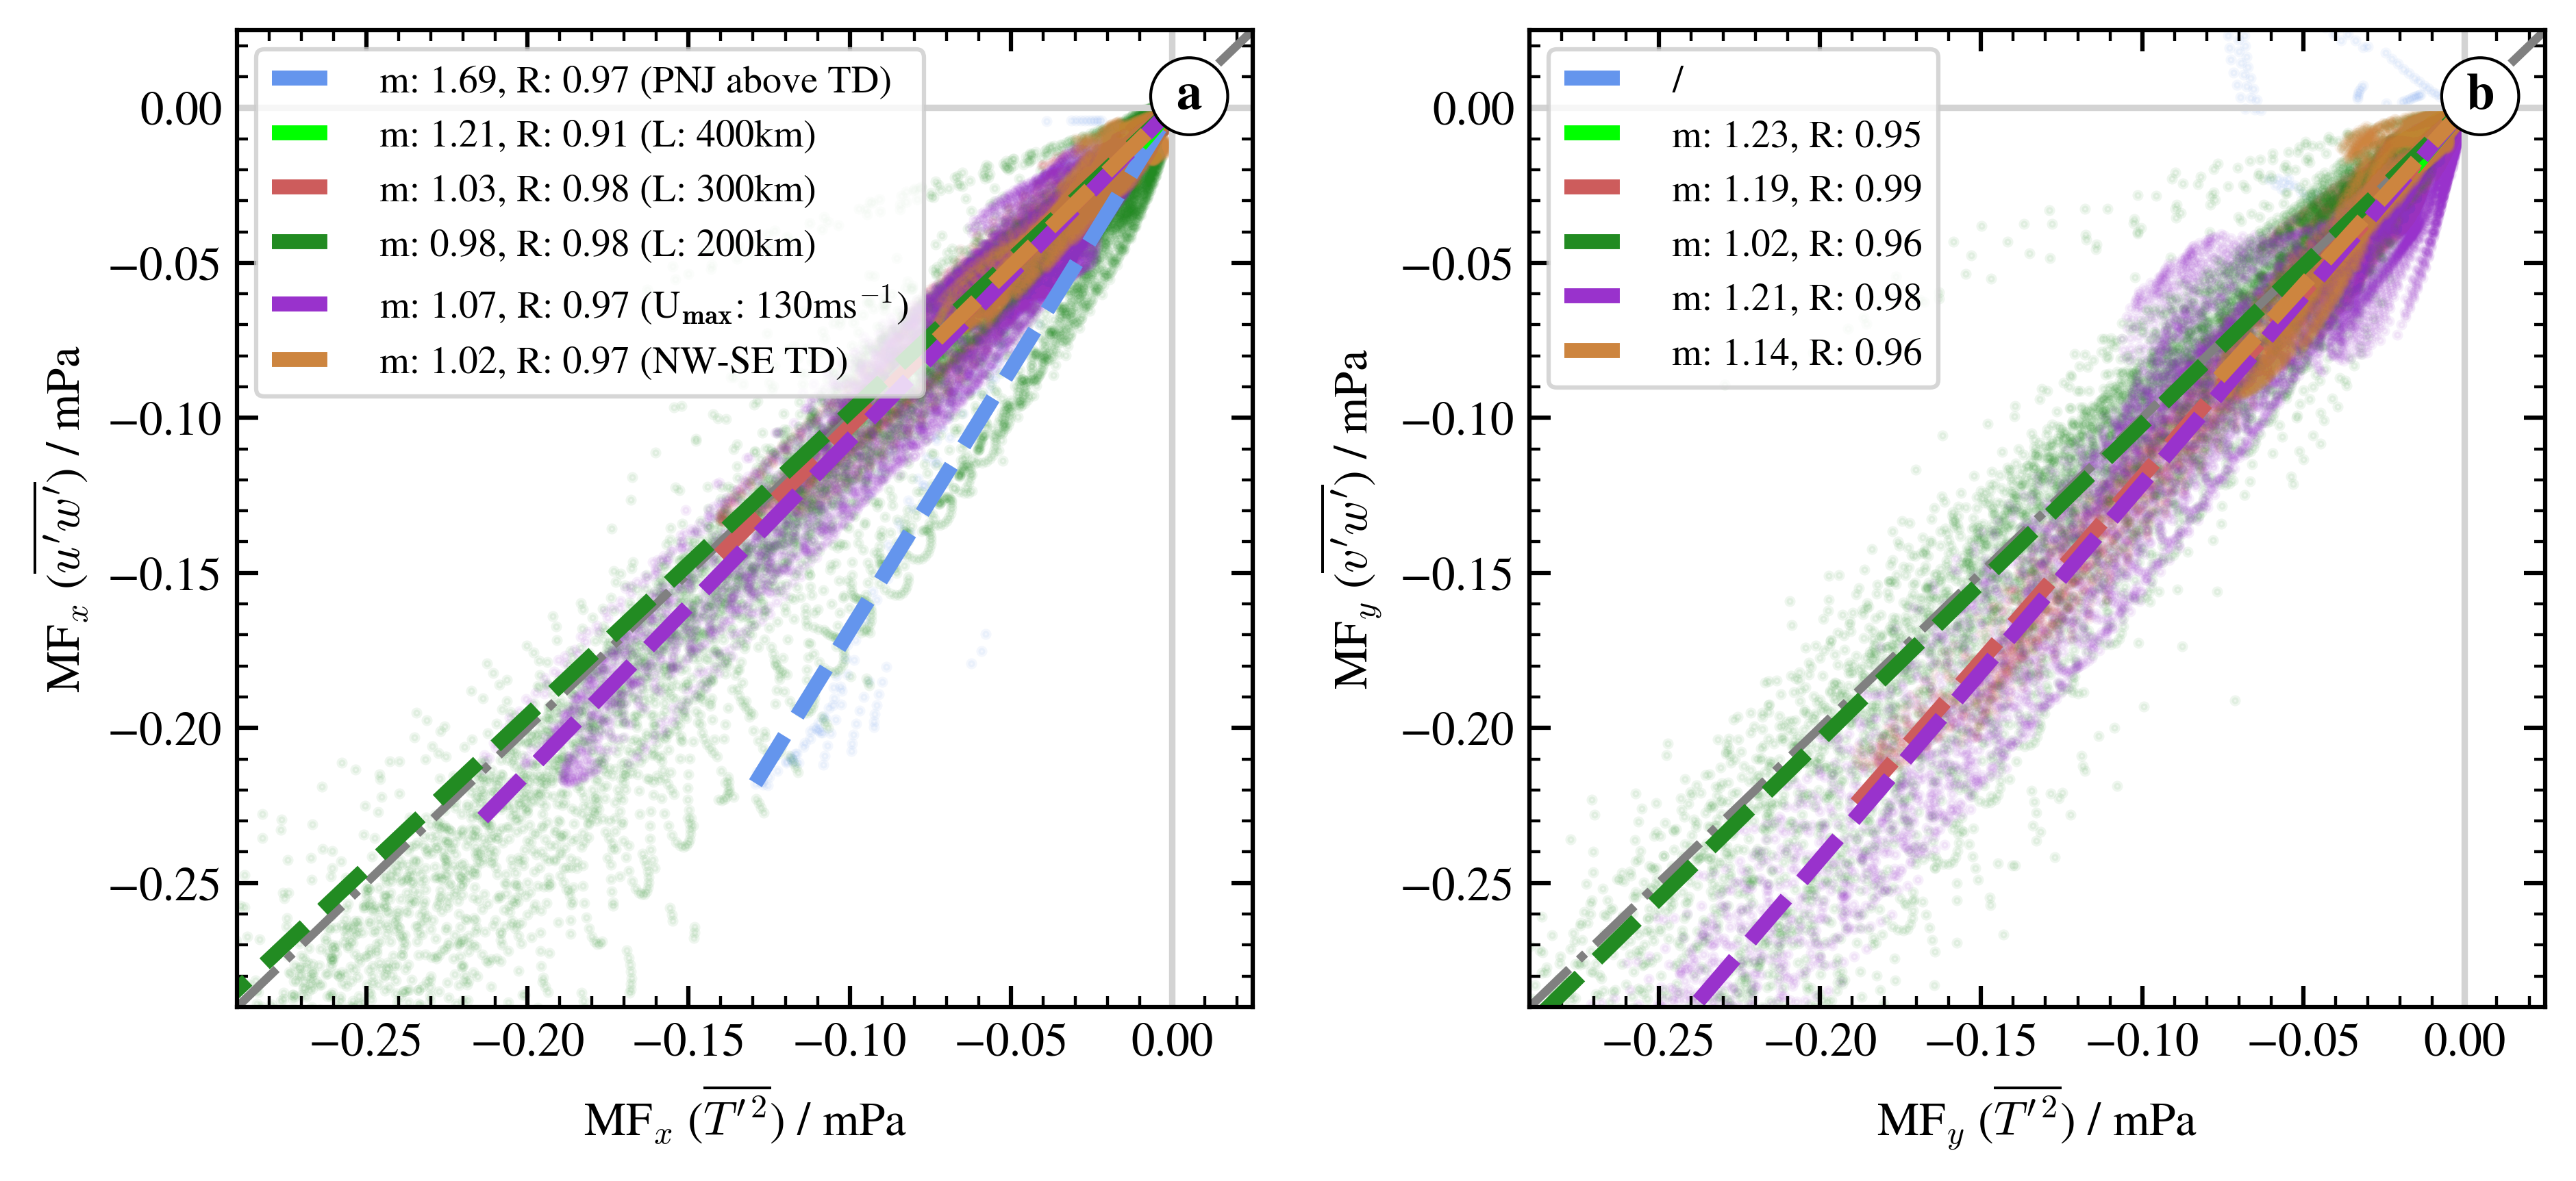
\includegraphics[width=0.99\textwidth]{figures_3D/waveletAna_mf_scatter.png}
    \caption{Scatter plots of the zonal (a) and meridional (b) MF at z=\SI{40}{\kilo\meter} after 72h for all simulations in Figure \ref{fig:waveletAna}. The x-axis refers to the MF calculated from temperature perturbations, the y-axis refers to the MF calculated from wind perturbations. Colored dashed lines are linear fits with slope m and intercept $y_{0}=0$ for each individual simulation.}
    \label{fig:mf_scatter}
\end{figure*}
Overall, momentum fluxes from wind and temperature correlate well. R values are greater than 0.9 for all simulations, so linear regressions in Figure \ref{fig:mf_scatter} represent meaningful relations. Especially linear fits of the zonal MF show a good agreement with slope values $m \approx 1$ with one exception. The slope of the linear regression for the simulation with the PNJ centered above the propagating tropopause depression has a slope of $m \approx 1.7$. In this simulation setup GWs propagate upward into the PNJ without a turning of phase lines resulting in no meridional flux. Most likely, this offset is related to nonlinear process at \SI{40}{\kilo\meter} that also lead to the partly unstructured wave pattern in Figure \ref{fig:waveletAna}a. The deviation from an infinitesimal depth of the tropopause depression and the utilization of an exponential damping in the vertical dimension could also contribute to the discrepancy from $m = 1$.

MF$_y$ (Figure \ref{fig:mf_scatter}b) also shows good agreement, but a general low bias of temperature-based with respect to wind-based MF can be observed. Only the simulation for the smallest depression width $L=\SI{200}{\kilo\meter}$ has an almost perfect slope while the general picture indicates $15-\SI{25}{\percent}$ higher values for MF$_y$ from winds.\\
MF$_x$ and MF$_y$ suggest a higher correlation for smaller depression widths $L$. Three simulations ($L=400,300,\SI{200}{\kilo\meter}$) are not enough to be conclusive here, but this trend could be related to the effect of rotation that becomes more relevant for wider tropopause folds that result in larger horizontal wavelengths and lower intrinsic frequencies $\hat{\omega}$. As discussed in the beginning of this section, the neglected factor $\textrm{A} \, \textrm{B}$ for the MF from $T'$ is not sensitive to large horizontal scales or an increased impact of Coriolis. On the other hand, the factor $\bigl(1-\frac{f^2}{\hat{\omega}^2}\bigr)$ in Equation \ref{equ:ps-mf} decreases for smaller $\hat{\omega}$, so MF from wind is overestimated, when this factor is neglected for low frequency waves with $\hat{\omega}$ approaching $f$. Maybe, it is this simplification under the midfrequency approximation that becomes less valid and leads to a higher MF from winds for wider tropopause folds.

Despite these uncertainties, we conclude that the calculation of MF from temperature perturbations leads to meaningful results for the spectrum of GWs excited by propagating tropopause depressions and research question 
\begin{tcolorbox}[]
    (R4) Can the MF of NOGWs above propagating tropopause depressions be calculated from temperature perturbations?
\end{tcolorbox}
can be answered with "Yes". Considering the uncertainty of real measurements the correspondence between temperature-based and wind-based MF is very good and uncertainties due to the calculation are tolerable. In addition, it shows that most of the GWs within the idealized simulations obey the polarization and dispersion relations of GWs and propagate virtually linearly up to an altitude of at least \SI{40}{\kilo\meter}. The analysis of horizontal cross-sections at lower levels leads to similar conclusions and is therefore left out.

% zero intercept was used, so larger fluxes might have stronger influence slope value??
% A particularly striking result is a widespread 

% The right part in Equation \ref{equ:mf-etot} fits to the work of \textcite[]{andrews_wave-action_1978} or the work of \textcite[]{fritts_spectral_1993} who derived energy spectra in the upper atmosphere from observations. 

% Vertical timeseries of temperature from Lidar observations usually aren't sufficient to derive horizontal momentum fluxes without additional information or assumptions for horizontal wavelengths.
% Gracile paper (Ern 2018) states a factor of Ekin/Epot = 5/3???? should be E0/Epot??
% $f$ is the inertial frequency
% p=5/3 (intrinsic frequency ωˆ spectrum of the GW wave energy density assumed to decrease with ωˆ−5/3)
% The acceleration or deceleration (X, Y ) of the background flow, in the following for simplification called gravity wave drag, is given by the vertical gradient of momentum flux: (X, Y ) = − 1 % ∂ (Fpx, Fpy ) ∂z , (12) with X and Y the drag in the zonal and meridional directions, respectively, and z the vertical coordinate.
 
% F = rho * k/m * Epot,max.
% Es gilt also Etot = Ekin + Epot = Epot,max (in Worten... zum Zeitpunkt, wo die potentielle Energie über die Schwingung maximal wird verschwindet der kinetische Anteil --> Ekin = 0). Wenn wir nun F allein aus den Temperaturvarianzen berechnen wollen nehmen wir an, dass
% Epot {gemittelt über eine Wellenperiode} = Ekin {gemittelt über eine Wellenperiode} (hier kommen dann wohl Annahmen wie linear und non-dissipative mit rein). Daraus folgt dann 
% --> Etot = 2 * Epot {gemittelt über eine Wellenperiode}
% --> F = rho * k/m * 2*Epot {gemittelt über eine Wellenperiode} = rho * k/m *(g/N)^2 * average((T'/T)^2)

\newpage
\thispagestyle{plain}

% ==== CHAPTER 6 ==============================================================
% ---- set some counters to zero:
\setcounter{equation}{0}
\setcounter{table}{0}
\setcounter{figure}{0}
% ---- include tex-file:
\chapter{NOGWs from propagating tropopause folds in ground-based Lidar observations}
% Lidar observations in Q3D simulations are not useful / used y position 1 instead on npy/2!! --> use local 2D simulations for analysis of these plots (eventually conduct constant wind simulations again)

Observations of GWs in the upper atmosphere (stratosphere and MLT) are sparse. AIRS on board of NASA’s Aqua satellite is presently the only instrument that provides temperature measurements for a limited altitude range applicable for the detection of GWs (e.g \cite[]{hindley_gravity_2019} or \cite[]{hindley_18year_2020}). Observations are available globally, but only on a daily basis and sensitive to just a portion of the gravity wave spectrum due to the so-called "observational filter" of the instrument properties (e.g. \cite[]{preusse_space-based_2002} or \cite[]{alexander_recent_2010}). Vertical temperature profiles from ground-based Lidar stations are currently the only alternative available on a regular basis. They provide much higher vertical and temporal resolution at the cost of being limited to a single location (point observation), night-time and clear sky conditions. The analysis of GWs in these measurements is challenging and at a certain point not possible without consulting additional information from other observations or model data. Thus, it is the goal of this chapter to provide a basis for identifying NOGWs from tropopause folds in these measurements and tackle the third research question of this thesis:

\begin{tcolorbox}[]
    (R4) Can NOGWs from propagating tropopause folds be identified in lidar observations?
\end{tcolorbox}
% Thus, representative patterns from theory or idealized studies are highly appreciated for their intepretation and
Though the proposed excitation mechanism of these NOGWs is supposed to mimic the excitation of MWs over topography, their appeareance in lidar observations might differ due to the propagation of their source. Therefore, section \ref{sec:lidOb-idealized} first deals with the question of how GWs generated by propagating tropopause depressions show up in vertical timeseries and how they could be interpreted utilizing the idealized simulations described in previous chapters.
Subsequently, section \ref{sec:lidOb-coral} presents two measurements of the Rayleigh Lidar CORAL (chapter \ref{sec:coral}) that show similar signatures as the idealized simulations. A first interpretation based on ERA5 reanalysis data is discussed, but it can be anticipated that further tools like for example high resolution simulations are needed to reach a conclusive interpretation. 


\section{Lidar observations in idealized numerical simulations}
\label{sec:lidOb-idealized}
% The goal of the following analysis is

% High resolution vertical time series at multiple locations were retrieved from the idealized numerical simulations discussed in previous chapters.

Wave properties of stationary mountain waves are somewhat unfavorable from a lidar observation point of view. Their horizontal phase speed vanishes ($c_{px}=0$) together with the ground-based frequency ($\omega$=0). As a result, phase lines in vertical time series of ground-based lidar observations appear horizontal and one can only derive the vertical wavelength $\lambda_z$ from the observations, but misses information on horizontal scales (e.g. \cite[]{dornbrack_interpretation_2017} or \cite[]{reichert_highcadence_2021}). Section \ref{sec:resultsQ3D} showed that NOGWs from a propagating source might develop similar properties, but within the reference frame moving with their source. Figure \ref{fig:lidar_sim} illustrates how this alters their appearance in vertical time series. As discussed in section \ref{sec:resultsQ3D}, the wave forcing of a trough moving with $c_{tf}$ (\ref{fig:lidar_sim}b) for a certain point in time can be reproduced by a stationary trough with a wind profile reduced by $c_{tf}$ (Figure \ref{fig:lidar_sim}c). However, phase lines in the vertical time series differ significantly and show an upward (downward) tilt for a source moving in the same (opposite) direction as the background wind (Figure \ref{fig:lidar_sim}d). The same feature can be observed for a more realistic wind profile with a tropopause jet and a polar night jet in Figure \ref{fig:lidar_sim}e and f (the reference simulation of chapter \ref{sec:resultsQ3D}). Does this allow for a derivation of horizontal wave properties? Yes and no! Clearly, tilted phase lines enable the quantification of a ground-based period $T$ from the vertical time series, but linking this period to wave properties depends on the wave source and atmospheric background conditions. Multiple phenomena could explain upward tilted phase lines in lidar observations, so their intepretation requires additional knowledge on the prevailing processes and synoptic situation. Examples are:
%  so by considering lidar observations only, upward tilted phase lines could for example be attributed
% \cite[]{ern_absolute_2004}

\begin{itemize}
    \item downward propagating wave packets caused by reflection or wave breaking in the upper atmosphere which excites secondary waves that travel up and down from their source region (\cite[]{dornbrack_interpretation_2017} and \cite[]{vadas_mechanism_2003}).
    % fishbone pattern

    \item transient background conditions. Mainly in the form of a varying wind speed and wind direction.

    \item a GW source moving in the same direction as the background wind as illustreated in Figure \ref{fig:lidar_sim}d and \ref{fig:lidar_sim}f.
\end{itemize}

\begin{figure*}[tbp]
    \centering
    \includegraphics[width=0.99\textwidth]{figures_lidar/lidana_th.png}
    \caption{Shown are vertical cross-sections (a,c,e) after $t$=\SI{72}{\hour} with vertical wind profiles in green and vertical time series (b,d,f) at the outlined position for three different simulations. The first simulation (a,b) features a stationary obstacle at the lower boundary and a constant wind profile. In the second simulation (c,d) the trough moves to the right with a constant speed $c_{tf}$=\SI{13.88}{\meter \per \second} and the wind is increased by the same amount. The last simulation (e,f) represents the reference simulation of the sensitivity analysis in section \ref{sec:resultsQ3D} with a more realistic stratospheric winter time wind profile. The assessment of $\lambda_z$ and period $T$ from the vertical time series is labeled in (d), two consecutive $\lambda_x$ are labeled in (c). Contour lines represent constant potential temperature and the amplitude of the lower boundary is scaled by a factor of 5.}
    \label{fig:lidar_sim}
\end{figure*}

For this work we continue with the last explanation and focus on the GW characterization for the simplified case of a constant wind profile shown in Figure \ref{fig:lidar_sim}c and \ref{fig:lidar_sim}d following the terminology and derivations of \textcite[]{gill_atmosphere-ocean_1982}, \textcite[]{fritts_gravity_2003} or \textcite[]{dornbrack_interpretation_2017}. To recap, a constant stratification with $N=\SI{0.02}{\per \second}$ was used for all simulations starting at the tropopause simplifying the dispersion relation for Boussinesq flows to
\begin{equation}
    \hat{w}^2 = N^2 \frac{k^2}{k^2+m^2} + f^2 \frac{m^2}{k^2+m^2}
    \label{equ_lid:dispersion}
    % observed waves obey a dispersion relation for internal Boussinesq
    % Alhough variations in density are the very essence of buoyancy, they are neglected everywhere in the Boussinesq equations “except in so far as they modify the action of gravity” (Rayleigh, 1916), i.e., the density is assumed to be constant except in the buoyancy force
    % by applying a peak finding algorith to the vertical profile and additionally a time span $T$ applying the same algorithm along the time axis
\end{equation}
with $\hat{w}$ being the intrinsic frequency and $f=$ \SI{-1.195e-4}{\per \second} the Coriolis parameter to consider the influence of Earth's rotation at a latitude of $55\degree$S. A constant background wind leads to a ground-based frequency
\begin{equation}
    w = \hat{w} + uk,
    % w = \hat{w} + uk = \frac{Nk}{\sqrt{k^2+m^2}}.
    \label{equ_lid:omega}
\end{equation}
and, in addition, \textcite{gill_atmosphere-ocean_1982} defines the useful aspect ratio
\begin{equation}
    \alpha = \frac{\text{vertical scale}}{\text{horizontal scale}} = \frac{\lambda_z}{\lambda_x} = \sqrt{\frac{\hat{w}^2-f^2}{N^2-\hat{w}^2}},
    \label{equ_lid:alpha}
\end{equation}
which simplifies the approximation of $\hat{w}$ for the relevant hydrostatic rotating wave regime to
\begin{equation}
    \hat{w}^2 \approx f^2 + N^2 \alpha^2.
    \label{equ_lid:omega_simp}
\end{equation}
As labeled in Figure \ref{fig:lidar_sim}d, the vertical distance between troughs or ridges in the vertical time series yields the vertical wavelength $\lambda_z=\SI{9.25}{\kilo \meter}$ and wavenumber $m$, the horizontal distance at \SI{40}{\kilo \meter} provides a period $T=\SI{13.92}{\hour}$ and ground-based frequency $\omega$. How can this frequency be interpreted? \textcite[]{dornbrack_interpretation_2017} clarify that in the presence of a background wind this question can only be answered by consulting further information or by proceding with assumptions. For the case of a propagating tropopause depression we can assume a stationary wave field within a reference frame that propagates with the depression. Then the tilt of the phase lines within the lidar observation depends on the propagation speed of the GW source and the horizontasl wavelength $\lambda_x$. A constant propagation speed $c_{tf}$=\SI{13.88}{\meter \per \second} leads to $\lambda_x = T \cdot c_{tf}$= \SI{695}{\kilo \meter}, which is in the range of wavelengths labeled in the vertical cross-section (Figure \ref{fig:lidar_sim}c) at the same height with $\lambda_x$=\SI{525}{\kilo \meter} - \SI{712}{\kilo \meter}. The ratio of $\lambda_x$ and $\lambda_z$ gives $\alpha=0.0133$ and it is possible to define the angle formed between lines of constant phase and the z-axis in real space
\begin{equation}
    \phi = \tan^{-1}(\frac{\lambda_x}{\lambda_z})=89.24\degree.
    \label{equ_lid:phi}
\end{equation}
From equation \ref{equ_lid:omega_simp} $\hat{w}\approx$ \SI{2.92e-4}, so $\hat{w}$ is of $\mathcal{O}(f)$ and $\hat{w}>=f$, which is in full compliance with the hydrostatic rotating wave regime described by \textcite[]{gill_atmosphere-ocean_1982}. It follows the intrinsic horizontal group velocity
\begin{equation}
    c_{gx} \approx \frac{N^2 \alpha}{m \sqrt{f^2+N^2 \alpha^2}} \approx \SI{-26.9}{\meter\per\second} 
    \label{equ_lid:cgh}
    % (phase propagation against the background wind results in a negative horizontal scale $k$ and, thus, negative $\alpha$)
\end{equation}
with a negative $m$ for upward propagating waves and the vertical group velocity
\begin{equation}
    c_{gz} \approx -\alpha c_{gx} \approx \SI{0.36}{\meter\per\second}
    \label{equ_lid:cgz}
\end{equation}
Again, this is in compliance with inertia-gravity waves in the hydrostatic rotating wave regime, where $c_{gx}$ does not compensate the background wind forcing. Knowing $U=\SI{45}{\meter\per\second}$ allows the calculation of $U_{force}=U-c_{tf}=\SI{31.12}{\meter\per\second}>\lvert c_{gx} \rvert$ indicating a leeward extend of the GWs with respect to the propagating tropopause fold. Considering the overlaying propagation with the fold the ground-based or extrinsic group velocity is $c_{Gx}=U+c_{gx}=\SI{18.1}{\meter\per\second}$ and following the assumptions above the ground-based horizontal phase speed has to be identical to the speed of the depression ($c_{Px} = c_{tf}$). \\
The vertical propagation of the GWs is independent of the background wind. It takes approximately 31 hours until they reach an altitude of 40km above the tropopause based on $c_{gz}$.

% First of all, there have to be sufficiently large tropospheric winds perpendicular to the mountain ridge for excitation of MWs (e.g., Bramberger et al., 2017; Dörnbrack et al., 1999; Kaifler, Kaifler, et  al.,  2015). In addition, Dörnbrack et  al.  (1999) report that good excitation conditions prevail when the wind turns no more than 30° within the first 30 km. Monthly mean wind speeds in ERA5 data are at about 𝐴𝐴 15 ms−1 at surface level (500 m) at all times. The wind rotation within the first 30 km is <30° during the months from March to October with a surface level forcing between 240° and 280°. Thus, in the climatological mean MWs are excited and able to propagate deep into the middle atmosphere in the winter months. A strong wind rotation within the first 30 km of about 60° can only be observed in July 2020. At this time, we also find reduced GW energies at all altitude regions (see Figure 6). For upward propagation, the wind speed in the direction of wave propagation must not become zero as this would lead to wave breaking (Lindzen,  1981). Moreover, for deep vertical propagation, the MWs should not encounter turning levels where the intrinsic frequency approaches the buoyancy frequency (e.g., Schoeberl, 1985). These conditions occur in the core of the PNJ and filter horizontally short MWs or lead to evanescent modes tunneling through the PNJ (e.g., Mixa et al., 2021). Another obstacle for MWs is the stratospheric wind minimum where the waves' 𝐴𝐴𝐴𝐴′-amplitude may become equal to the horizontal wind speed causing wave breaking. This wind minimum can act as a valve for vertically propagating MWs (Kruse et al., 2016). Figure 10 reveals that low wind speeds at ∼25 km altitude occur from March to May. In the winter months, with positive temperature gradients (Figure 2) and large horizontal wind speeds (Figure 10) up to 50 km, generally good vertical propagation conditions can be expected. Above, shear instabilities and unstable lapse rates lead to wave dissipation. On the other hand, the mesosphere is the favorable region for the generation of secondary gravity waves (Heale et al., 2020; Kogure et al., 2020; Vadas & Becker, 2019; Vadas et al., 2018). Large contributions of apparently up- and downward propagating waves and reduced contributions of stationary waves (see Table 3) at mesospheric altitudes might indicate their existence above Río Grande.

\section{Signatures of NOGWs from propagating tropopause folds in CORAL measurements}
\label{sec:lidOb-coral}

Ater a detailed investigation of the proposed excitation mechanism for NOGWs above tropopause folds through idealized numerical simulations, this section goes one step further and tries to identify the pattern of these GWs (discussed in the Section \ref{sec:lidOb-idealized}) in actual lidar measurements of the stratosphere and mesosphere. Ideally, this lidar station would be located within the latitude band of the PNJ around \SI{60}{\degree S} to ensure relevant excitation and propagation conditions. And it should be far away from orography to eliminate the superposition of MWs and NOGWs. Since 2018 the Compact Autonomous Rayleigh Lidar (CORAL) of the DLR conducts measurements at the southern tip of South America (\SI{53.79}{\degree S}) in Río Grande, Argentina (Section \ref{sec:coral}). It's automatic operation provides a unique dataset of observations within the relevant latitude band, but its proximity to the Andes Mountains is not a coincidence. It is a very appropriate location to study Earth's GW hot spot with large amplitude MWs (\cite[]{rapp_southtrac-gw_2021} or \cite[]{reichert_highcadence_2021}). As so often, reality is not ideal. Nevertheless, it might still be possible to identify signatures of NOGWs from propagating tropopause folds in these lidar measurements, even though MWs dominate CORAL's measurements. Hereafter, two CORAL observations are selected that show similar patterns as the vertical timeseries of the idealized simulations, more specifically, upward tilted phase lines. 

Figure \ref{fig:coral_2018} and Figure \ref{fig:coral_2020} show temperature measurements for a night in June 2018 and a night in August 2020. A background state $\bar{T}$ and perturbations $T'$ are obtained by applying a vertical highpass Butterworth filter with a cutoff wavelength of $\lambda_{z,cut}=\SI{20}{\kilo\meter}$. Though multiple studies suggest $\lambda_{z,cut}=\SI{15}{\kilo\meter}$ for MWs, we adapt to the results of \textcite[]{reichert_robert_characterization_2022}, who discovered that more than \SI{50}{\percent} of the waves in the relevant CORAL dataset exhibit vertical wavelengths larger than \SI{16.5}{\kilo\meter}. Most likely a result of the very strong horizontal winds of the PNJ above Río Grande in austral winter.
%%% first case (2018)
\begin{figure*}[tbp]
    \centering
    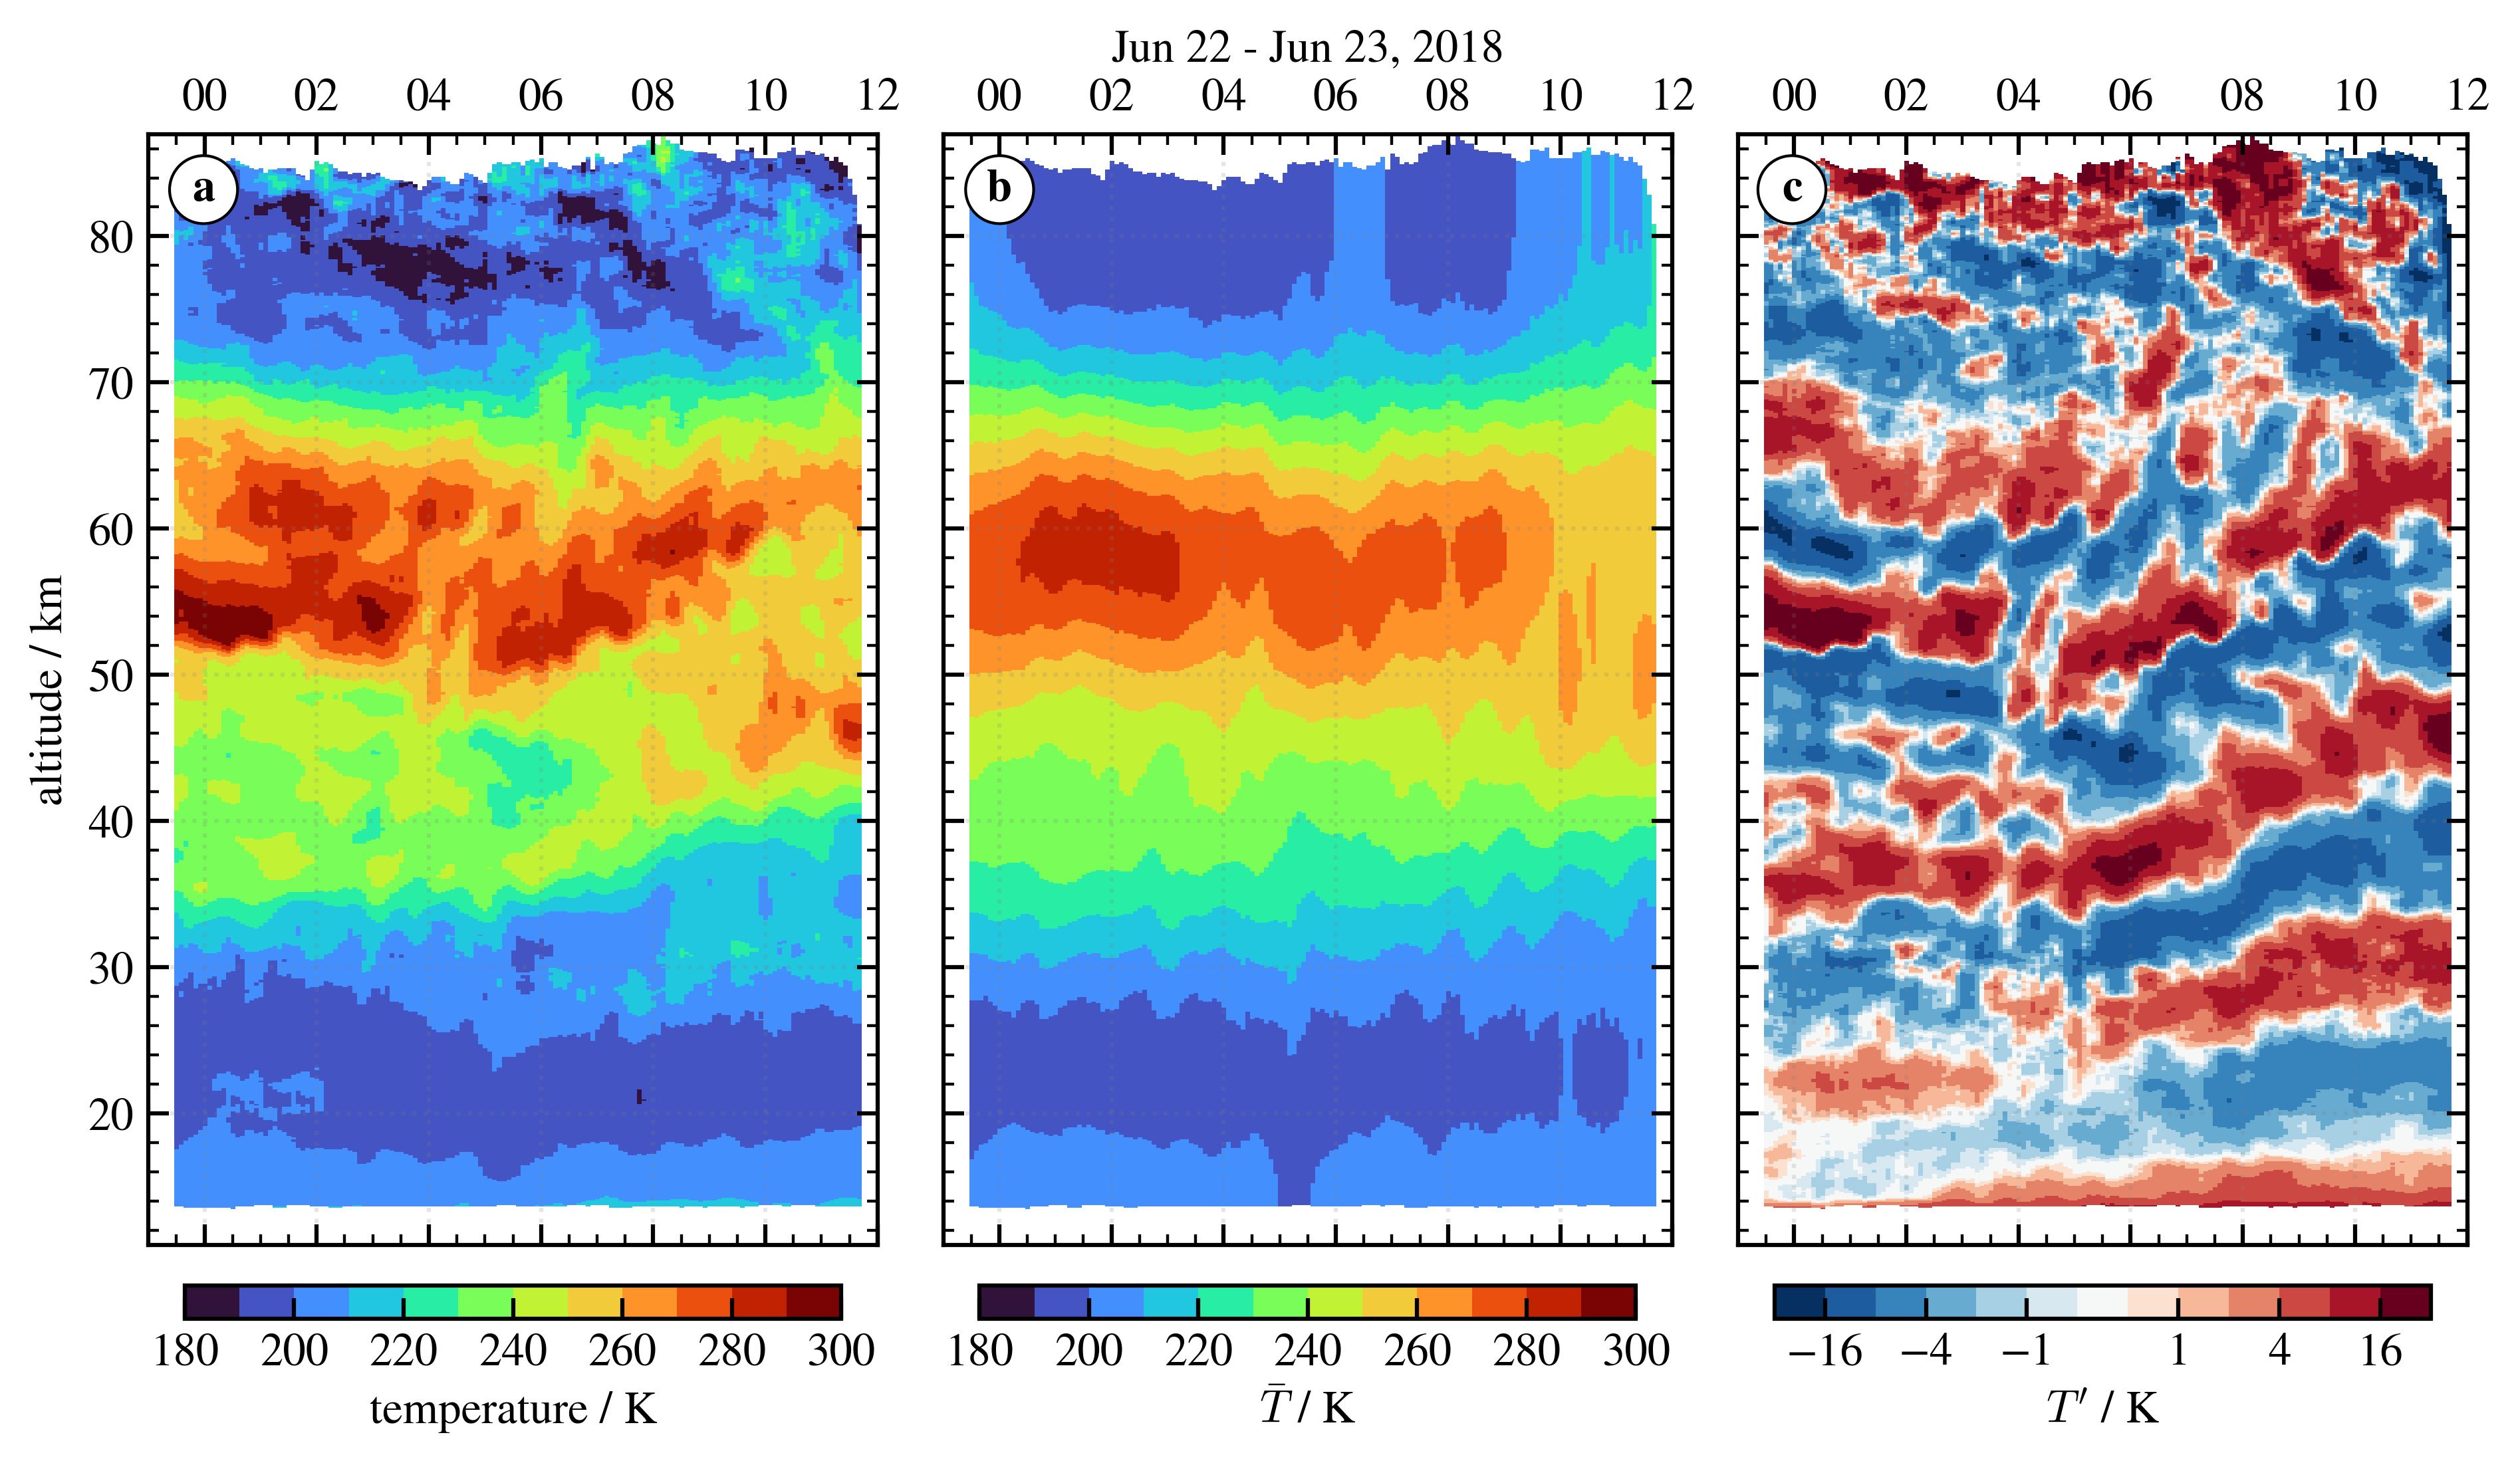
\includegraphics[width=0.99\textwidth]{figures_lidar/coral_event_20180622.png}
    \caption{Nighttime temperature measurements of CORAL located in Río Grande, Argentina (\SI{53.79}{\degree S}, \SI{67.75}{\degree W}) from the 22nd to the 23rd of June 2018. Shown are retrieved temperature profiles (a), background temperature profiles $\bar{T}$ after applying a vertical high-pass Butterworth filter with a cutoff wavelength of $\lambda_{z,cut}=\SI{20}{\kilo\meter}$ (b) and temperature perturbations $T'=T-\bar{T}$ (c).}
    \label{fig:coral_2018}
\end{figure*}
%%% second case (2020)
\begin{figure*}[tbp]
    \centering
    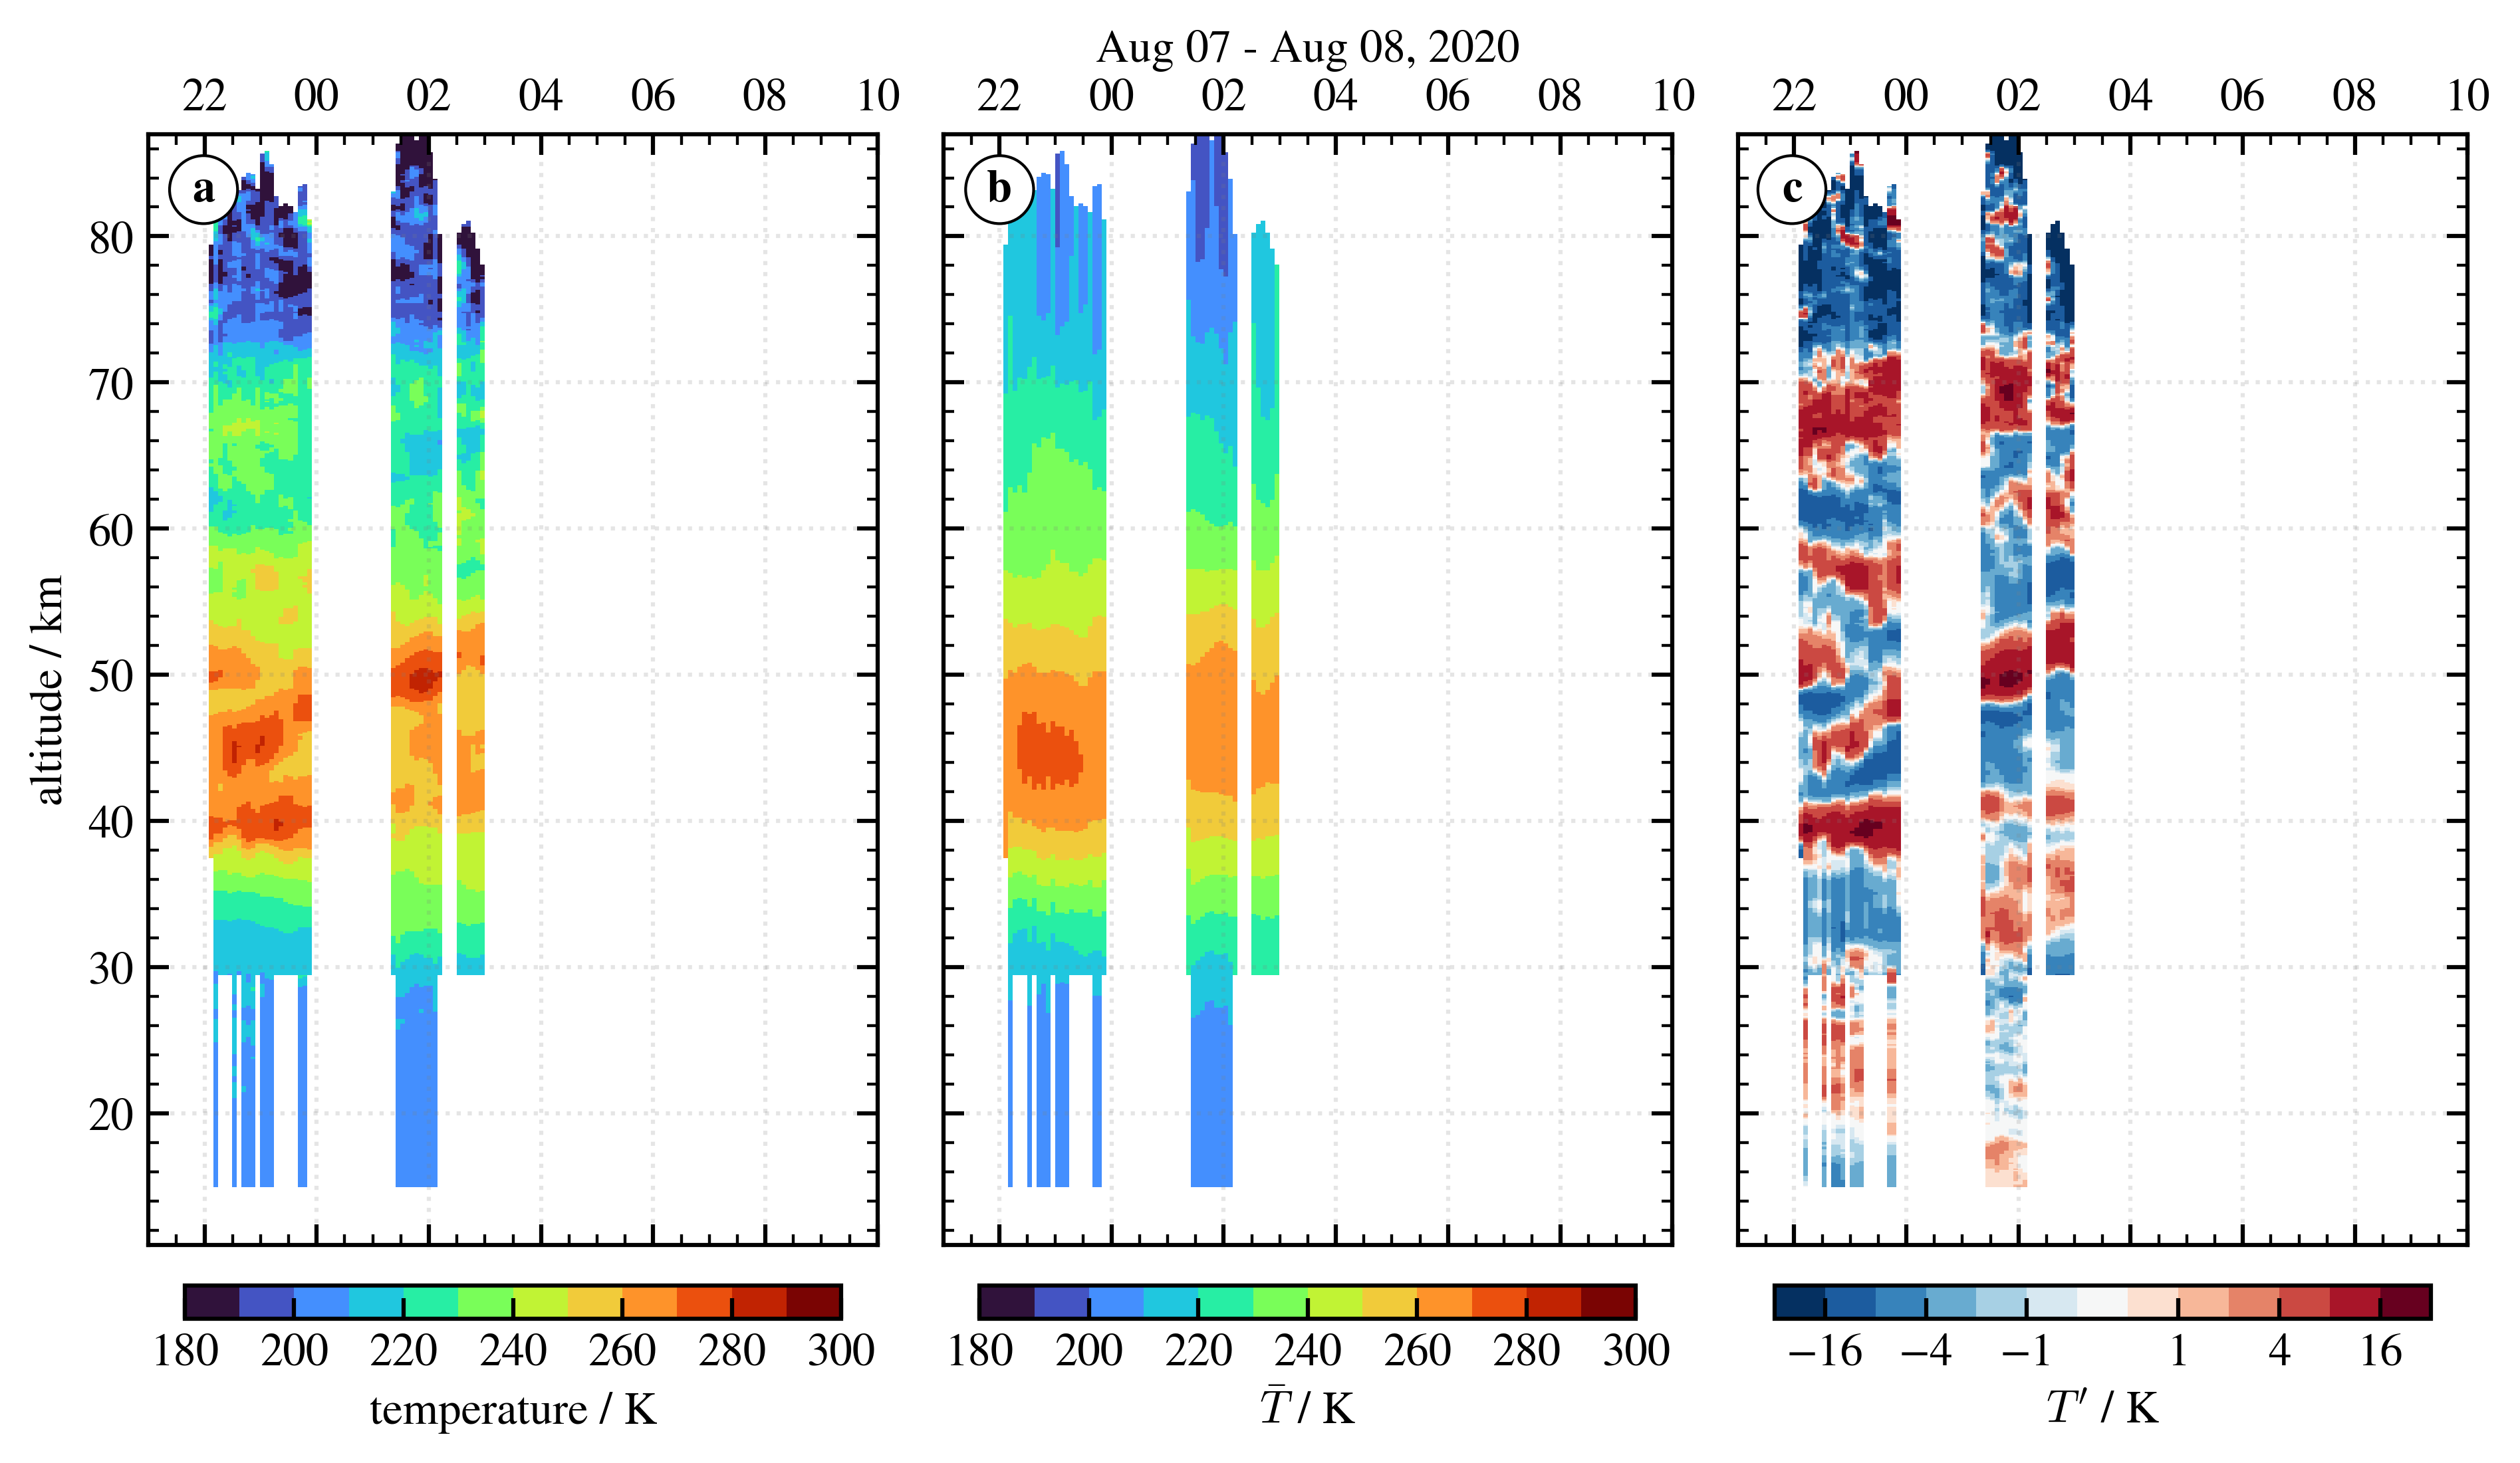
\includegraphics[width=0.99\textwidth]{figures_lidar/coral_event_20200807.png}
    \caption{Identical to Figure \ref{fig:coral_2018} showing nighttime measurements from the 7th to the 8th of August 2020. Periods of missing data are related to cloud coverage.}
    \label{fig:coral_2020}
\end{figure*}
In the first measurement (Figure \ref{fig:coral_2018}c), upward tilted phase lines are clearly observed after 05:00 UTC. Horizontal phase lines before 05:00 UTC might indicate that these waves are related to a MW event with non-stationary processes, but a more detailed analysis of the synoptic situation is essential for further interpretations. The same is true for the second observation. Again Figure \ref{fig:coral_2020}c shows upward tilted phase lines, in this case most pronounced between 40 and \SI{60}{\kilo\meter}. Unfortunately, this night was temporarily cloudy at Río Grande preventing a continuous measurement, but it might as well be promising, if these clouds are related to a passing frontal system and a tropopause fold on the larger scale. To support further interpretations of the measurements concise overviews of the available ERA5 data follow.

Similar figures (Figure \ref{fig:era5_2018} and \ref{fig:era5_2020}) are presented for both CORAL measurements that try to reproduce the measurements in the ERA5 data (a), visualize GW activity in the stratosphere (b and c) and corresponding dynamics at tropopause level (d, e and f). In addition, wind and geopotential height at \SI{850}{hPa} in (f) provide an idea on the prevailing forcing conditions for MWs in the same figure. \\
We note that phase lines in both vertical timeseries (a) tilt upward for the period of the observations. It strongly suggests that the processes that lead to the upward tilt in both CORAL measurements are represented in the ERA5 data and covered sufficiently in the dynamics of the underlying IFS model. Taking a closer look at each case can be instructive.
%%% Is ERA5 based on 9km IFS model runs???
%%% OVERLAY CORAL MEASUREMENTS WITH CONTOUR LINES IN ERA5 DATA
%%% - state that vertical time series would look quite similar to observations - angle of idealized simulation for realistic wind profile -> approximately 20km / 12h 
%%% change butterworth to pcolormesh instead of contourf
%%% change color of CORAL to black or darkgrey

\subsection*{ERA5 overview for June 22nd/23rd, 2018 measurements}
\begin{figure*}[tbp]
    \centering
    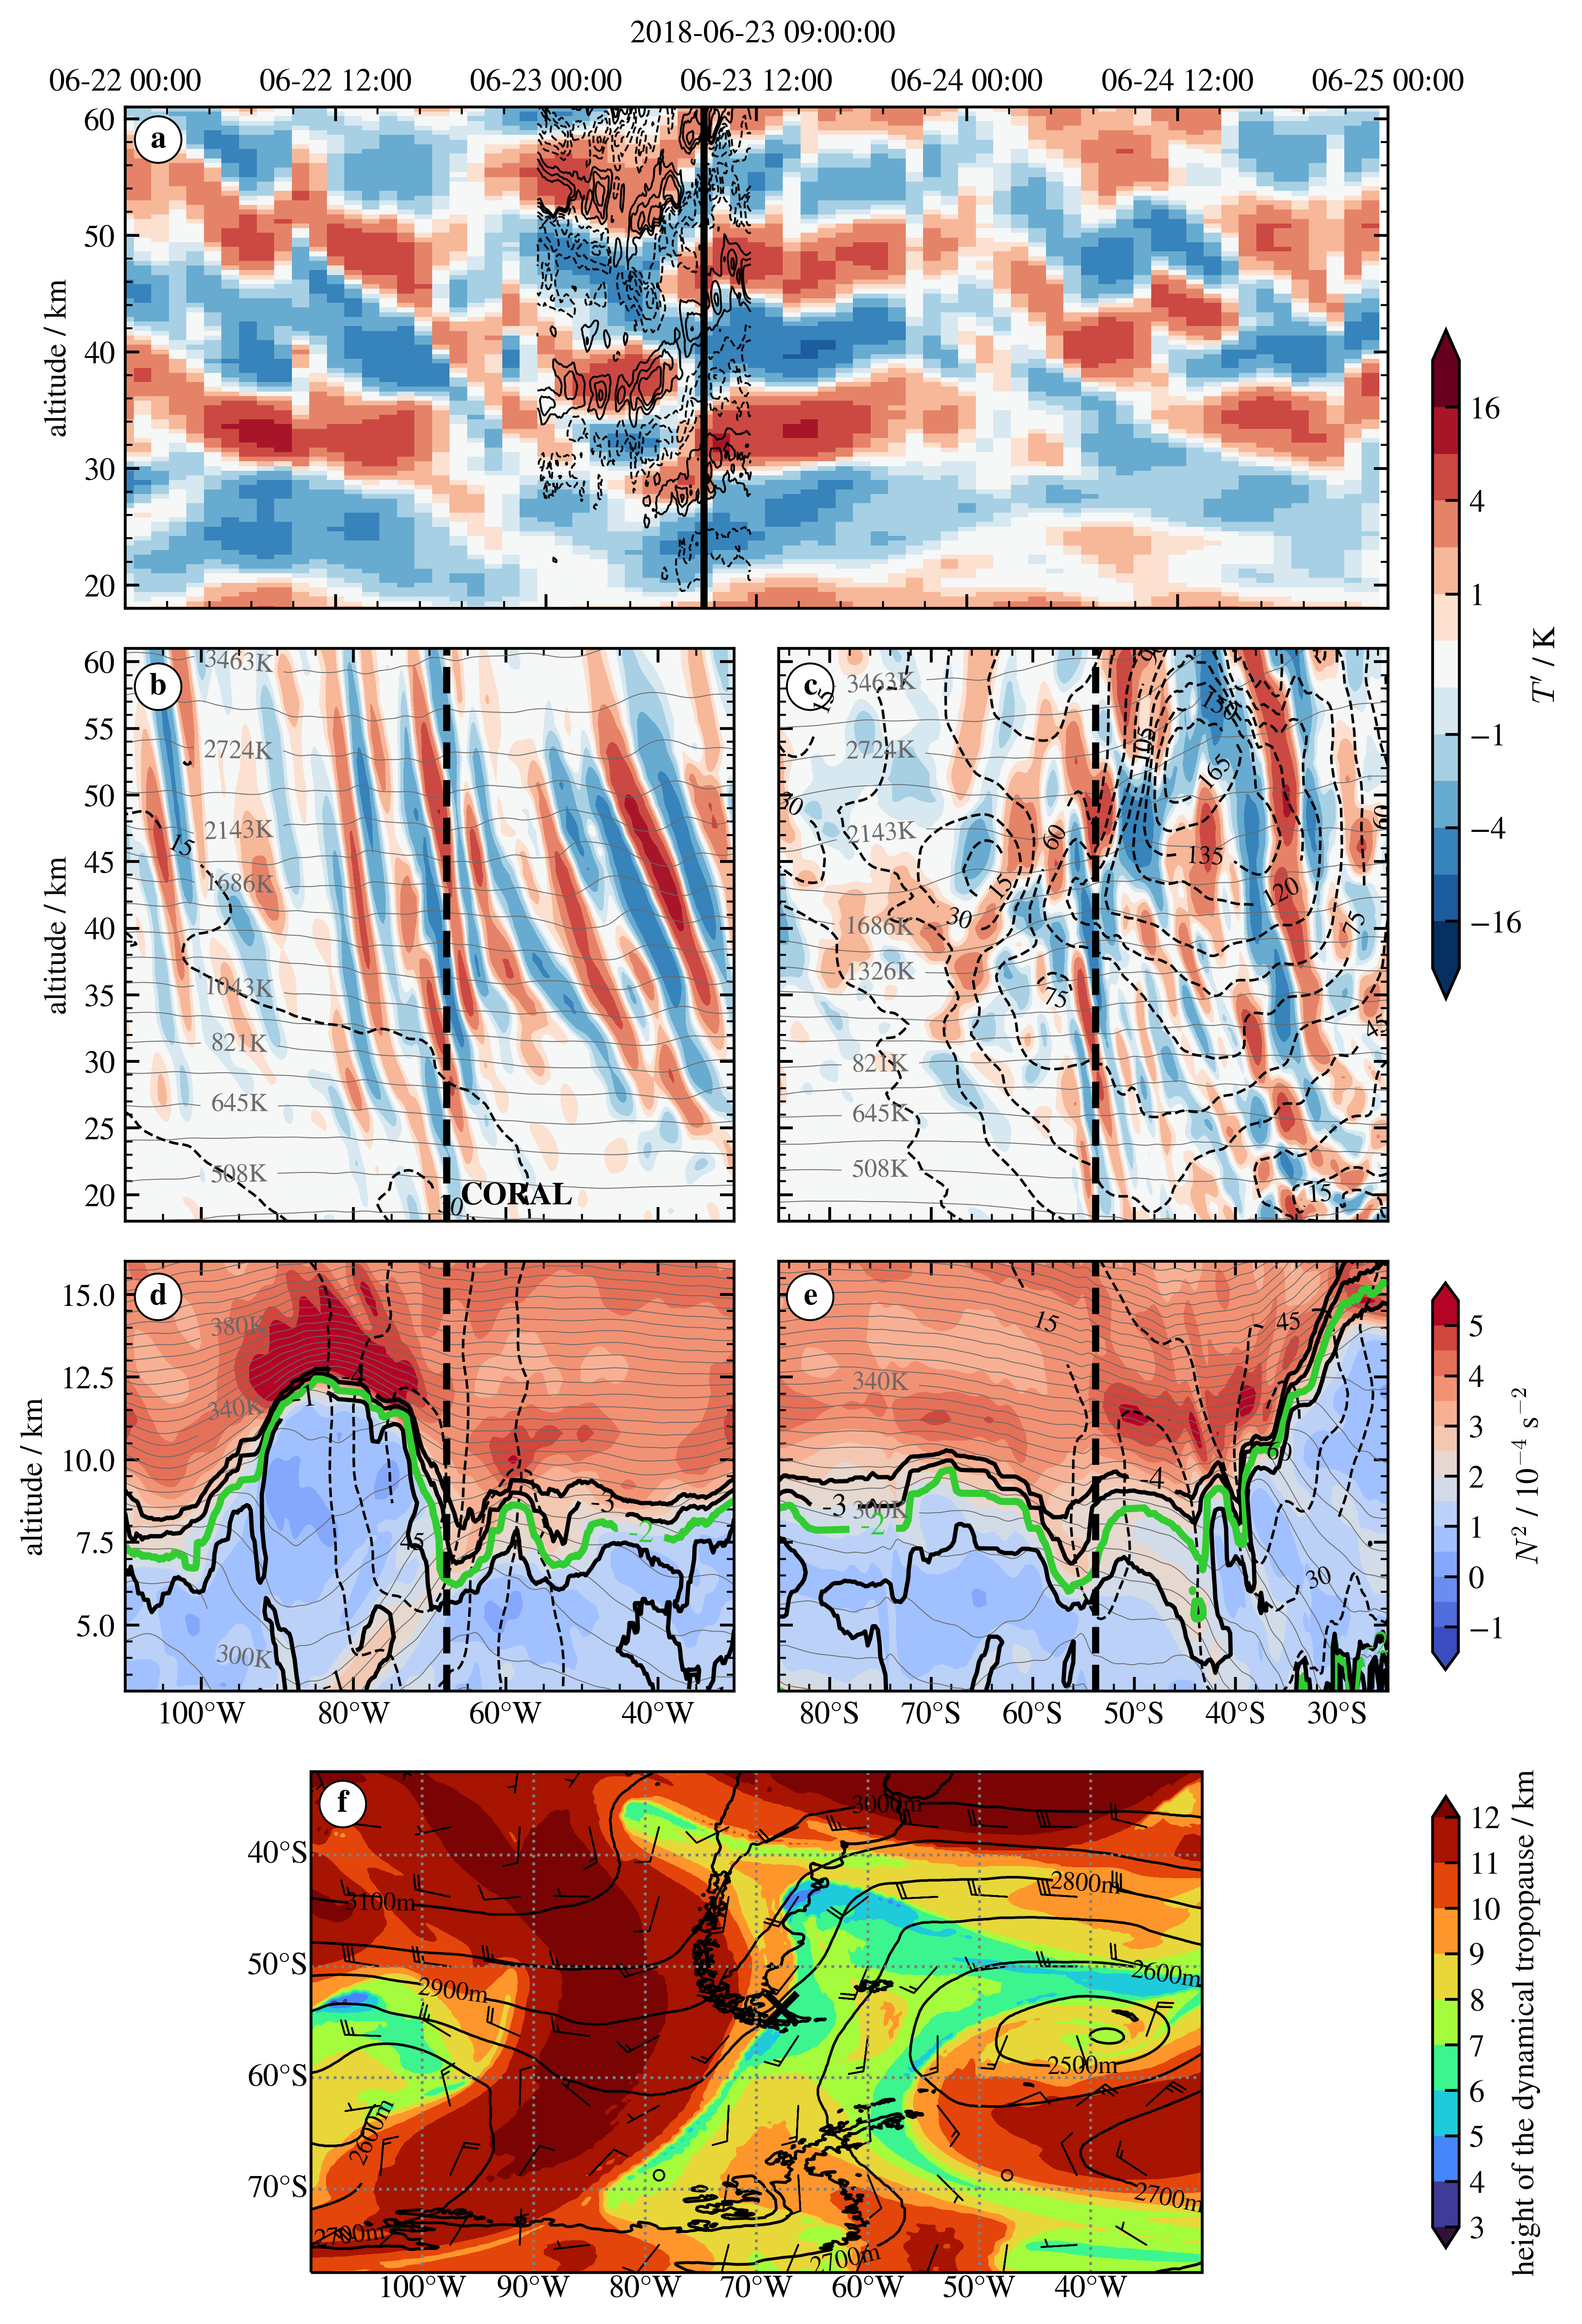
\includegraphics[width=0.8\textwidth]{figures_lidar/era5_trop_strat_33.png}
    \caption{ERA5 data overview for the first CORAL measurement from the 22nd to the 23rd of June 2018. (a) shows vertical profiles of stratospheric temperature perturbations for CORALs location after applying a vertical butterworth filter similar to the measurements (Figure \ref{fig:coral_2018}c). (b) and (c) show vertical cross sections of stratospheric temperature perturbations (after applying a horizontal Gaussian filter) for the latitude (b) and longitude (c) of CORAL. (d) and (e) show corresponding vertical cross sections at tropopause level with thick lines indicating PVU levels 1-4 (2 in green) and $N^2$ color coded to differentiate between tropospheric and stratospheric air. Dashed lines in the vertical cross sections show zonal ((c) and (e)) and meridional ((b) and (d)) winds. (f) shows the height of the dynamical tropopause in a horizontal cross section for the \SI{2}{PVU} level color coded with geopotential height and wind barbs for the \SI{850}{hPa} level. The vertical line in (a) marks the time for (b)-(f).}
    % The vertical line in (a) marks the time for (b)-(f) and CORAL's location is highlighted in the vertical cross-sections (b)-(e) and with a cross in (f).
    \label{fig:era5_2018}
\end{figure*}
At first, we want to find out if a tropopause fold could be the reason for the upward tilted phase lines in Figure \ref{fig:coral_2018}c. The vertical cross sections at tropopause level (Figure \ref{fig:era5_2018}d and e) show vanishing structures of a tropopause fold, but preceding timestamps clearly illustrate that the fold's core already passed CORAL \SI{24}{h} earlier. Blue colors northeast of CORAL in (f) indicate the position of the fold during the observations, too. Signatures of upward tilted phase lines in the extended vertical timeseries (Figure \ref{fig:era5_2018}a) and in the measurements appear significantly after the passage of the fold. It appears that in this case the phase line pattern is not caused by NOGWs above a tropopause fold. Can alternative processes be identified in the ERA5 data? \\
During the observation a strong negative PV anomaly (centered around \SI{85}{\degree W} in (d)) with a substantial warm air mass below (dark red area in (f)) approaches CORAL. On the southern hemisphere warm air advection is accompanied by wind backing, which can be observed in (f) over multiple timesteps, too. The large scale wind direction around CORAL changes from south to southwest at lower levels resulting in a transient wind forcing. It then transitions into a quite stationary regime favoring the excitation of MWs at the southernmost mountain range of the Andes, the Cordillera Darwin. The vertical timeseries in (a) supports this interpretation. The upward tilted phase lines transition into horizontal phase lines that persist for almost \SI{12}{h} subsequent to the period of the CORAL measurements. A clear sign for stationary MWs. In addition, phase lines in (b) and (c) around \SI{20}{\kilo\meter} and above indicate the propagation of MWs excited southwest of CORAL's location, too. \\
All in all, these observations in the ERA5 data draw a conclusive picture and suggest that the upward tilt of phase lines in the first CORAL measurement (Figure \ref{fig:coral_2018}c) is caused by a transient wind forcing with wind backing resulting in non-stationary MWs for a about \SI{6}{h}.
%% exceptionally strong PNJ with significant shift of PNJ to the north for that point in time
%% check spacing of paragraphs of proposal
%% apparently
\subsection*{ERA5 overview for August 7th/8th, 2020 measurements}
\begin{figure*}[tbp]
    \centering
    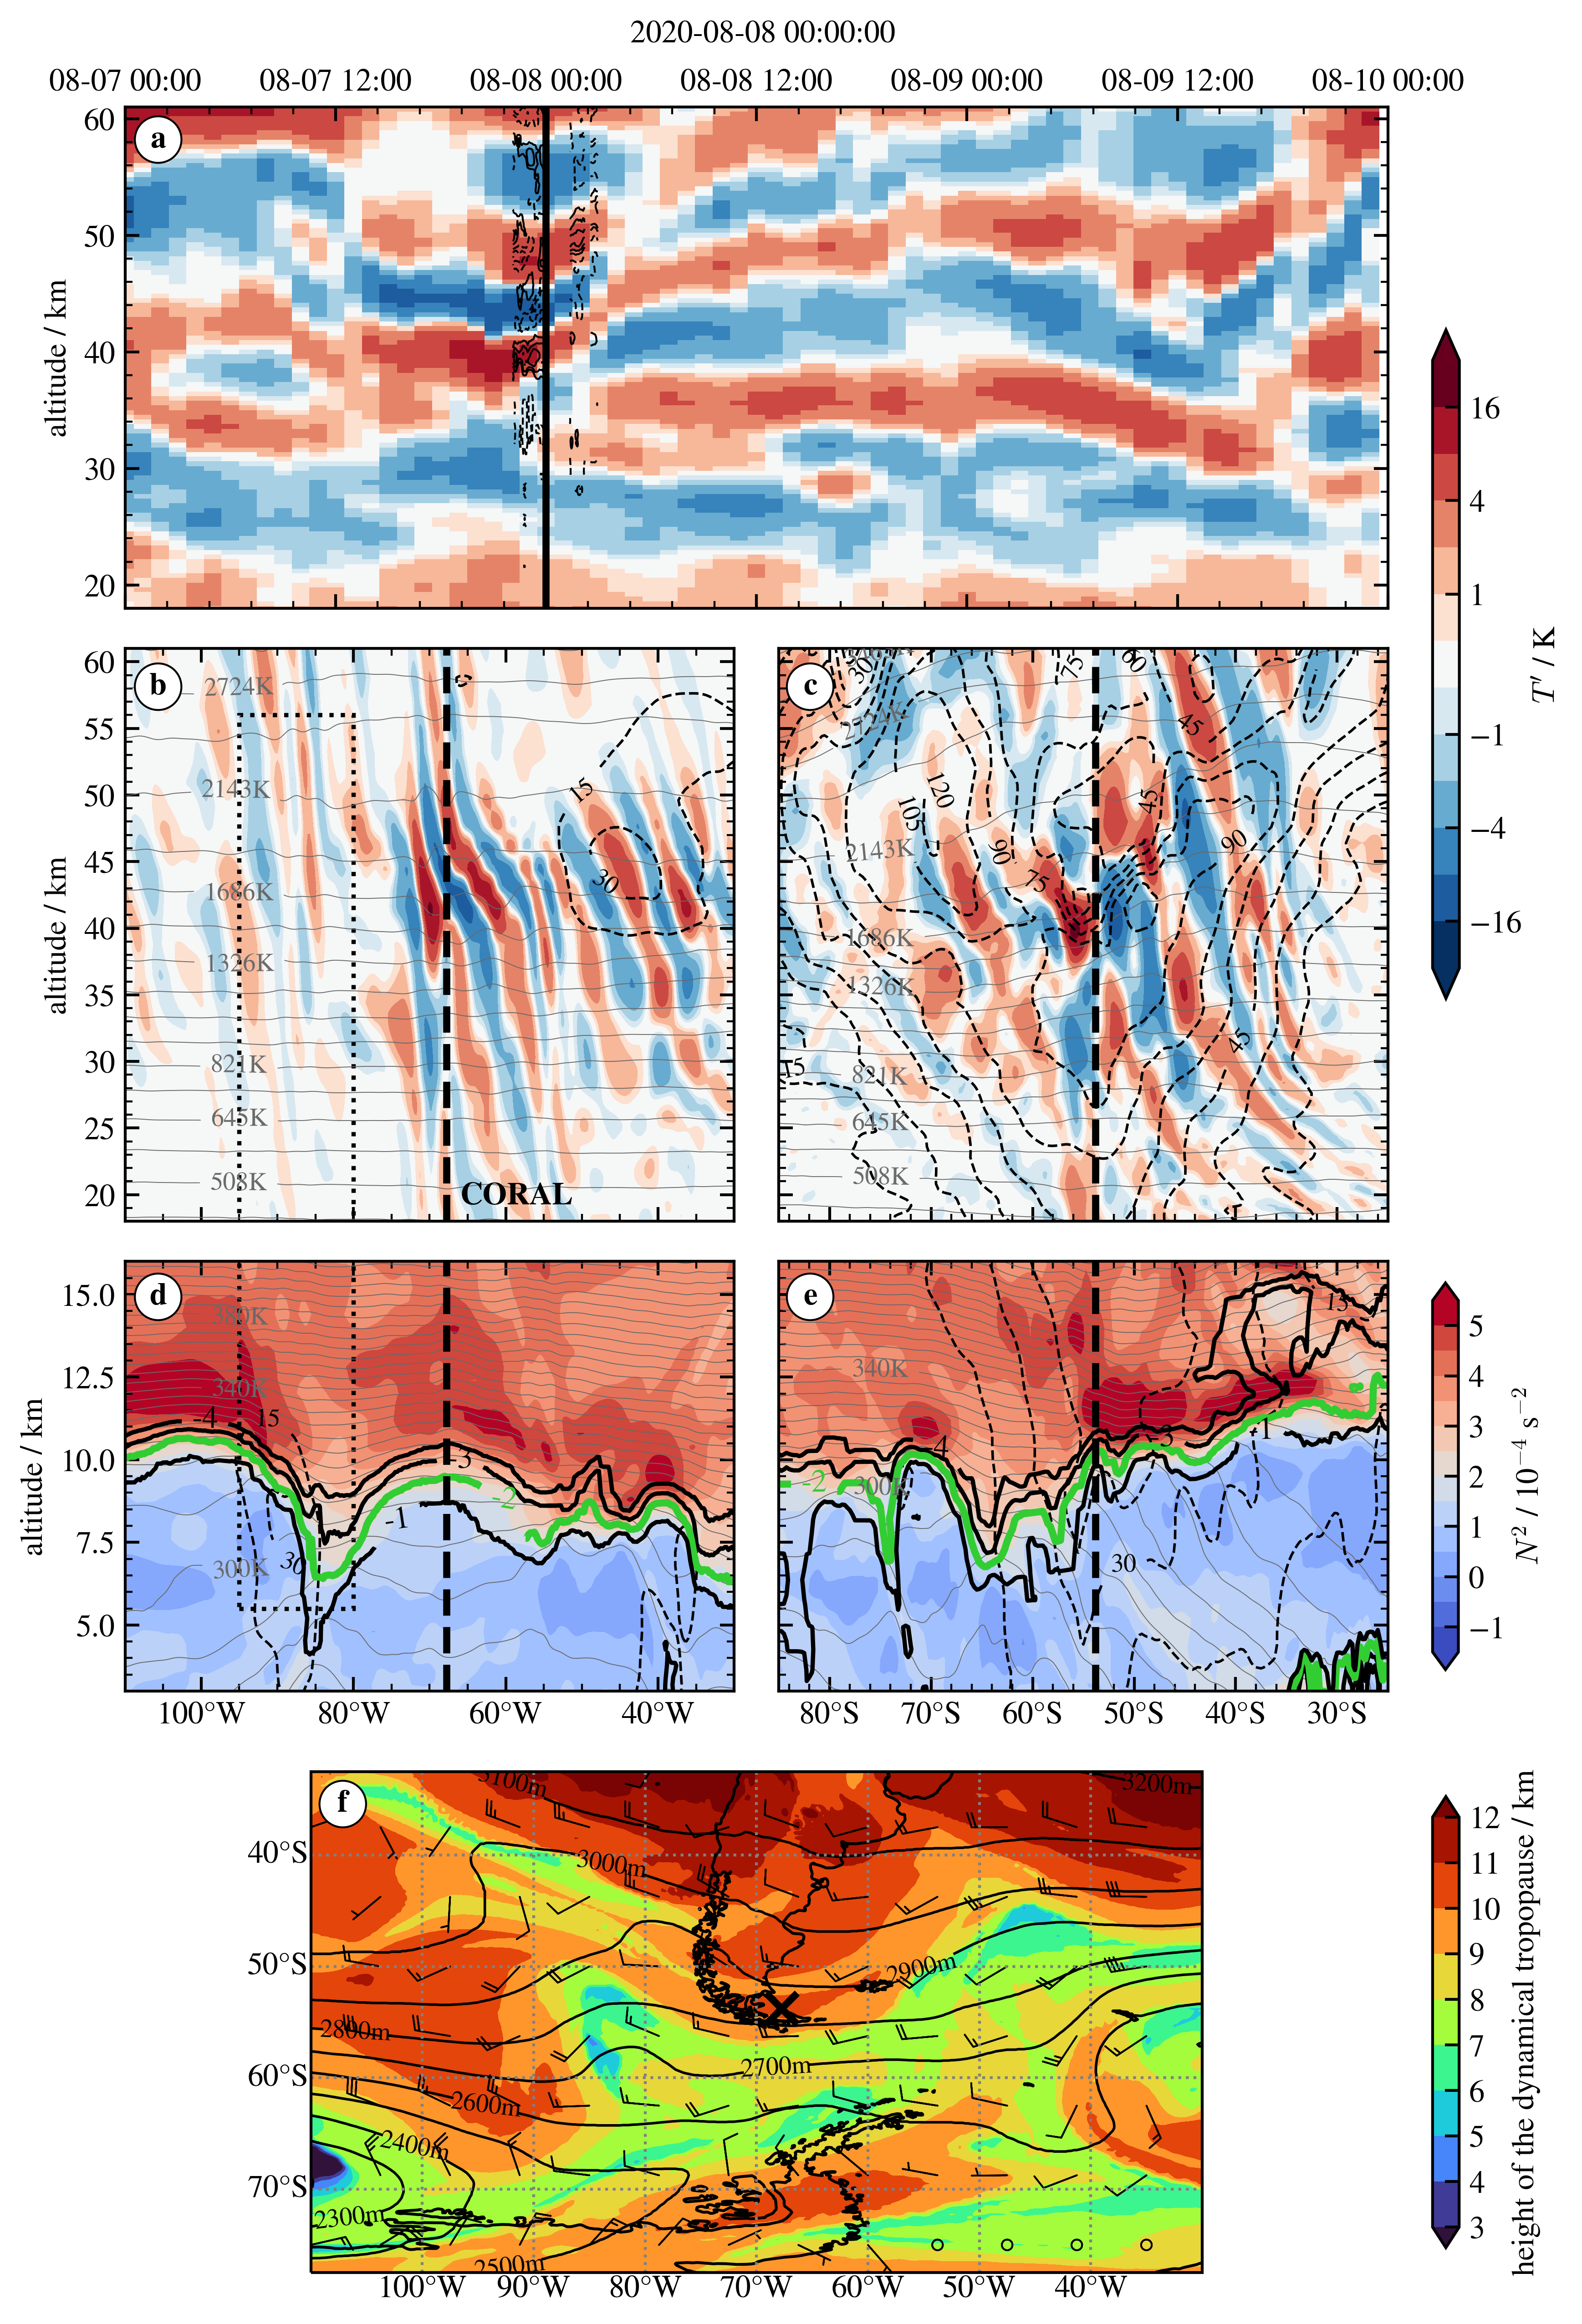
\includegraphics[width=0.8\textwidth]{figures_lidar/era5_trop_strat_24.png}
    \caption{Identical to Figure \ref{fig:era5_2018} showing an overview of ERA5 data for the second CORAL measurement from the 7th to the 8th of August 2020.}
    \label{fig:era5_2020}
\end{figure*}
Again, we first check for the presence of a tropopause fold during the CORAL observation. The PVU levels in (d) and greenblue colors in (f) of Figure \ref{fig:era5_2020} indicate the development of a textbook tropopause fold west of CORAL at \SI{85}{\degree W}, but once more, the timing of its pass over CORAL does not fit to the measurements. The significant upward tilt of phase lines in (a) between approximately 21:00 and 04:00 UTC appears earlier than the pass of the depression around 17:00 UTC. Could a transient wind forcing explain the upward tilt once again? \\
As depicted in the meridional cross section (c) the PNJ is centered directly above CORAL for this event. Considering the horizontal refraction of GWs into the jet discussed in chapter \ref{sec:results3D}, phase lines observed in the extended vertical timeseries in (a) at higher alitudes might actually belong to sources further north or south. Phase lines in (c) suggest that waves observed with CORAL above \SI{40}{\kilo\meter} originate further north from latitudes around 40-\SI{50}{\degree S}. The Andes Mountains align nearly exactly in a north-south direction in this latitude band and are a reliable source for MWs. In fact, the direction and speed of the prevailing wind in (f) that flows over the Andes in that area changes its direction before and during the period of the observations. Speed increases and the wind transitions from a westerly to a more northwesterly flow (wind veering like in the first event). However, conditions are not as distinct as in the first case. Wind speed and direction at lower levels continue to change afterwards and another feature in the ERA5 data should be noted. \\
Meridional winds in (b) show a wind veering from a westerly towards a more southwesterly flow between 40 and \SI{60}{\kilo\meter} and 35 to \SI{50}{\degree W}. This meandering of the PNJ passed CORAL around 19:00 UTC, so just three hours before CORAL started its measurements. When observing the phase lines in (b) for multiple timesteps a compression of the vertical wavelengths can be observed, which seems to follow the meandering of the PNJ. This fits to the upward tilted phase lines in (a). The vertical wavelengths decrease towards the end of the upward tilt before they increase again. \\
In conclusion, the interpetation of the ERA5 data is not as clear for the second CORAL measurement. GWs above a propagating tropopause fold can be ruled out as the source for the upward tiled phase lines, but alternative processes are not fully conclusive, too. Nevertheless, transient wind conditions close to the ground that relate to the forcing conditions and transient conditions of the PNJ are likely the reason for the upward tilt.
% With some imagination phase lines still turn upward...

\section{Summary and answer to research question (R4)}
\label{sec:lidOb-summary}
This chapter focused on relating the theoretical foundations from previous chapters to potential measurements in the real atmosphere. More specifically, the goal was to utilize the idealized numerical simulations of this work to identify patterns of NOGWs from propagating tropopause folds in lidar measurements to answer the third research question of this thesis:

\begin{tcolorbox}[]
    (R4) Can NOGWs from propagating tropopause folds be identified in observations?
\end{tcolorbox}

Vertical timeseries were presented to mimic the measurement of a ground-based lidar in the idealized simulations. These showed a clear pattern for GWs from a propagating source (e.g. a tropopause fold) with upward tilted phase lines. The angle of the tilt depends on the propagation speed of the source and the horizontal wavelength of the GW. Thus, it should be possible to detect NOGWs from propagating tropopause folds in lidar observations from a theoretical point of view. \\
In a next step, we checked measurements of the lidar system CORAL from the southern tip of South America and presented two observations that include the pattern of upward tilted phase lines in the lidar data. \\
However, upward tilted phase lines in vertical timeseries can not only result from a progating GW source. Other processes that result in a similar pattern are for example downward propagating GWs or transient atmospheric conditions during the excitation or propagation of the GWs. Therefore, it was the goal of analysing corresponding ERA5 data to pinpoint the processes that led to the signatures in the measurements. \\
The analysis revelead that tropopause folds were not causing the upward tilted phase lines in both case studies, but transient background conditions and MWs. Most likely a lidar location less influenced by MWs could reveal if the discussed signatures can be identified above propagating tropopause folds and the proposed excitation process exists in the real world.

To conclude, theory and idealized numerical simulations present a clear pattern of NOGWs from propagating tropopause folds that can be identified in observations. In practice though, it can be challenging to relate these signatures of GWs in lidar measurements to explicit processes in the real atmosphere. Additional information from models is needed and, up to today, it was not possible to utilize observations to confirm the excitation process of NOGWs above tropopause folds proposed in this thesis and in \textcite[]{dornbrack_stratospheric_2022}.
%% Overall conclusion:
% No matter what the escitation process for NOGWs is, they would be much easier derived in lidar data far away from orography, because the superposition with MWs can be ruled out.
% Waves can be observed in vertical cross section above tropopause fold in era5 like in doernbrack paper
% theoretically yes - practically not confirmed
% include characterisation of NOGWs from folds in research question????
\newpage
\thispagestyle{plain}

% ==== CONCLUSIONS =============================================================
% ---- set some counters to zero:
\setcounter{equation}{0}
\setcounter{table}{0}
\setcounter{figure}{0}
% ---- include tex-file:
\chapter{Conclusion}

Summarize answers from all subsections without restating the research questions

2D analysis
- A reference wind speed (wind in total column - spped of transient lower boundary) can be used to generate similar wave pattern in stationary reference frame

- conclusion from 2D cases -> transfer of stationary mountain wave analysis

3D analysis
- Background conditions in stratosphere can result in wave pattern observed in Figure from intro the case study by \cite{dornbrack_stratospheric_2022} during RF 25 of the DEEPWAVE campaign.
- Spectrum fits in terms of observed wavelenghts

% Wavelength discussion:
% AIRS data:
% Sensitivity is close to 100 percent for waves with wavelengths between 35 and 45 km in the vertical and less than around 500 km in the horizontal, and around 50 percent for wavelengths greater than 17 km in the vertical and less than 1000 km in the horizontal. The majority of our measured wavelengths in the results of this study fall within this 50 percent sensitivity region (as we would expect),

% Regarding the GW belt we have to consider that AIRS is mainly sensitive to vertical wavelengths larger than 17km. These wavelengths almost exclusively occure in the vicinity of the northern or southern PNJ due to the refraction of MWs or NOGWs into the jet. The jet favors the propagation of GWs towards higher altitudes (stratosphere/mesosphere), but on the other side the transformation of the wave properties leads to a significant influence of the istrument's observational filter.
% \textcite[]{hindley_gravity_2019} show that  


Same conclusion as many studies that oblique propagation of GW is significant and has to be improved in GCMs. Parameterisations like recent from Eichinger,...


% However, the belt of increased flux over the Southern Ocean shown in Ern et al. (2018) appears to be compara- tively more pronounced during June to August in their study than we observe here in AIRS measurements. The observa- tional filter of limb-sounding instruments means that they are more sensitive to gravity waves with relatively short ver- tical wavelengths (∼ 3–15 km) and relatively long horizon- tal wavelengths (∼ 500–5000 km). This suggests that a sig- nificant part of the oceanic section of the belt of enhanced gravity wave activity at 60◦ S is made up of long-horizontal wavelength waves, to which AIRS is less sensitive. \cite[]{hindley_gravity_2019}

% Critical assumption 
% Ina (ECMWF 1km simulation) suggests that gravity wave belt difference is associated with <100km waves
% What wavelengths are suggested based on AIRS data


%%%%%%%%%%%%% \chapter{Outlook} %%%%%%%%%%%%%%

Outlook

- Further analysis of ground-based lidar data

- full 3D simulations (cite zhang.. 2005 together with Alexander/Durran...) extend those simulations to upper stratosphere.

- tropospheric and stratospheric flows


\newpage
\thispagestyle{plain}


% ==== APPENDIX ================================================================
% ---- start appendix:
\appendix
% ---- set some counters to zero:
\setcounter{equation}{0}
\setcounter{table}{0}
\setcounter{figure}{0}
% ---- include tex-file:
\chapter{Supporting figures of the wavelet analysis and momentum flux calculation in Chapter \ref{sec:results3D}}
\label{appA}
\thispagestyle{plain}
%
\begin{figure*}[tbp]
    \centering
    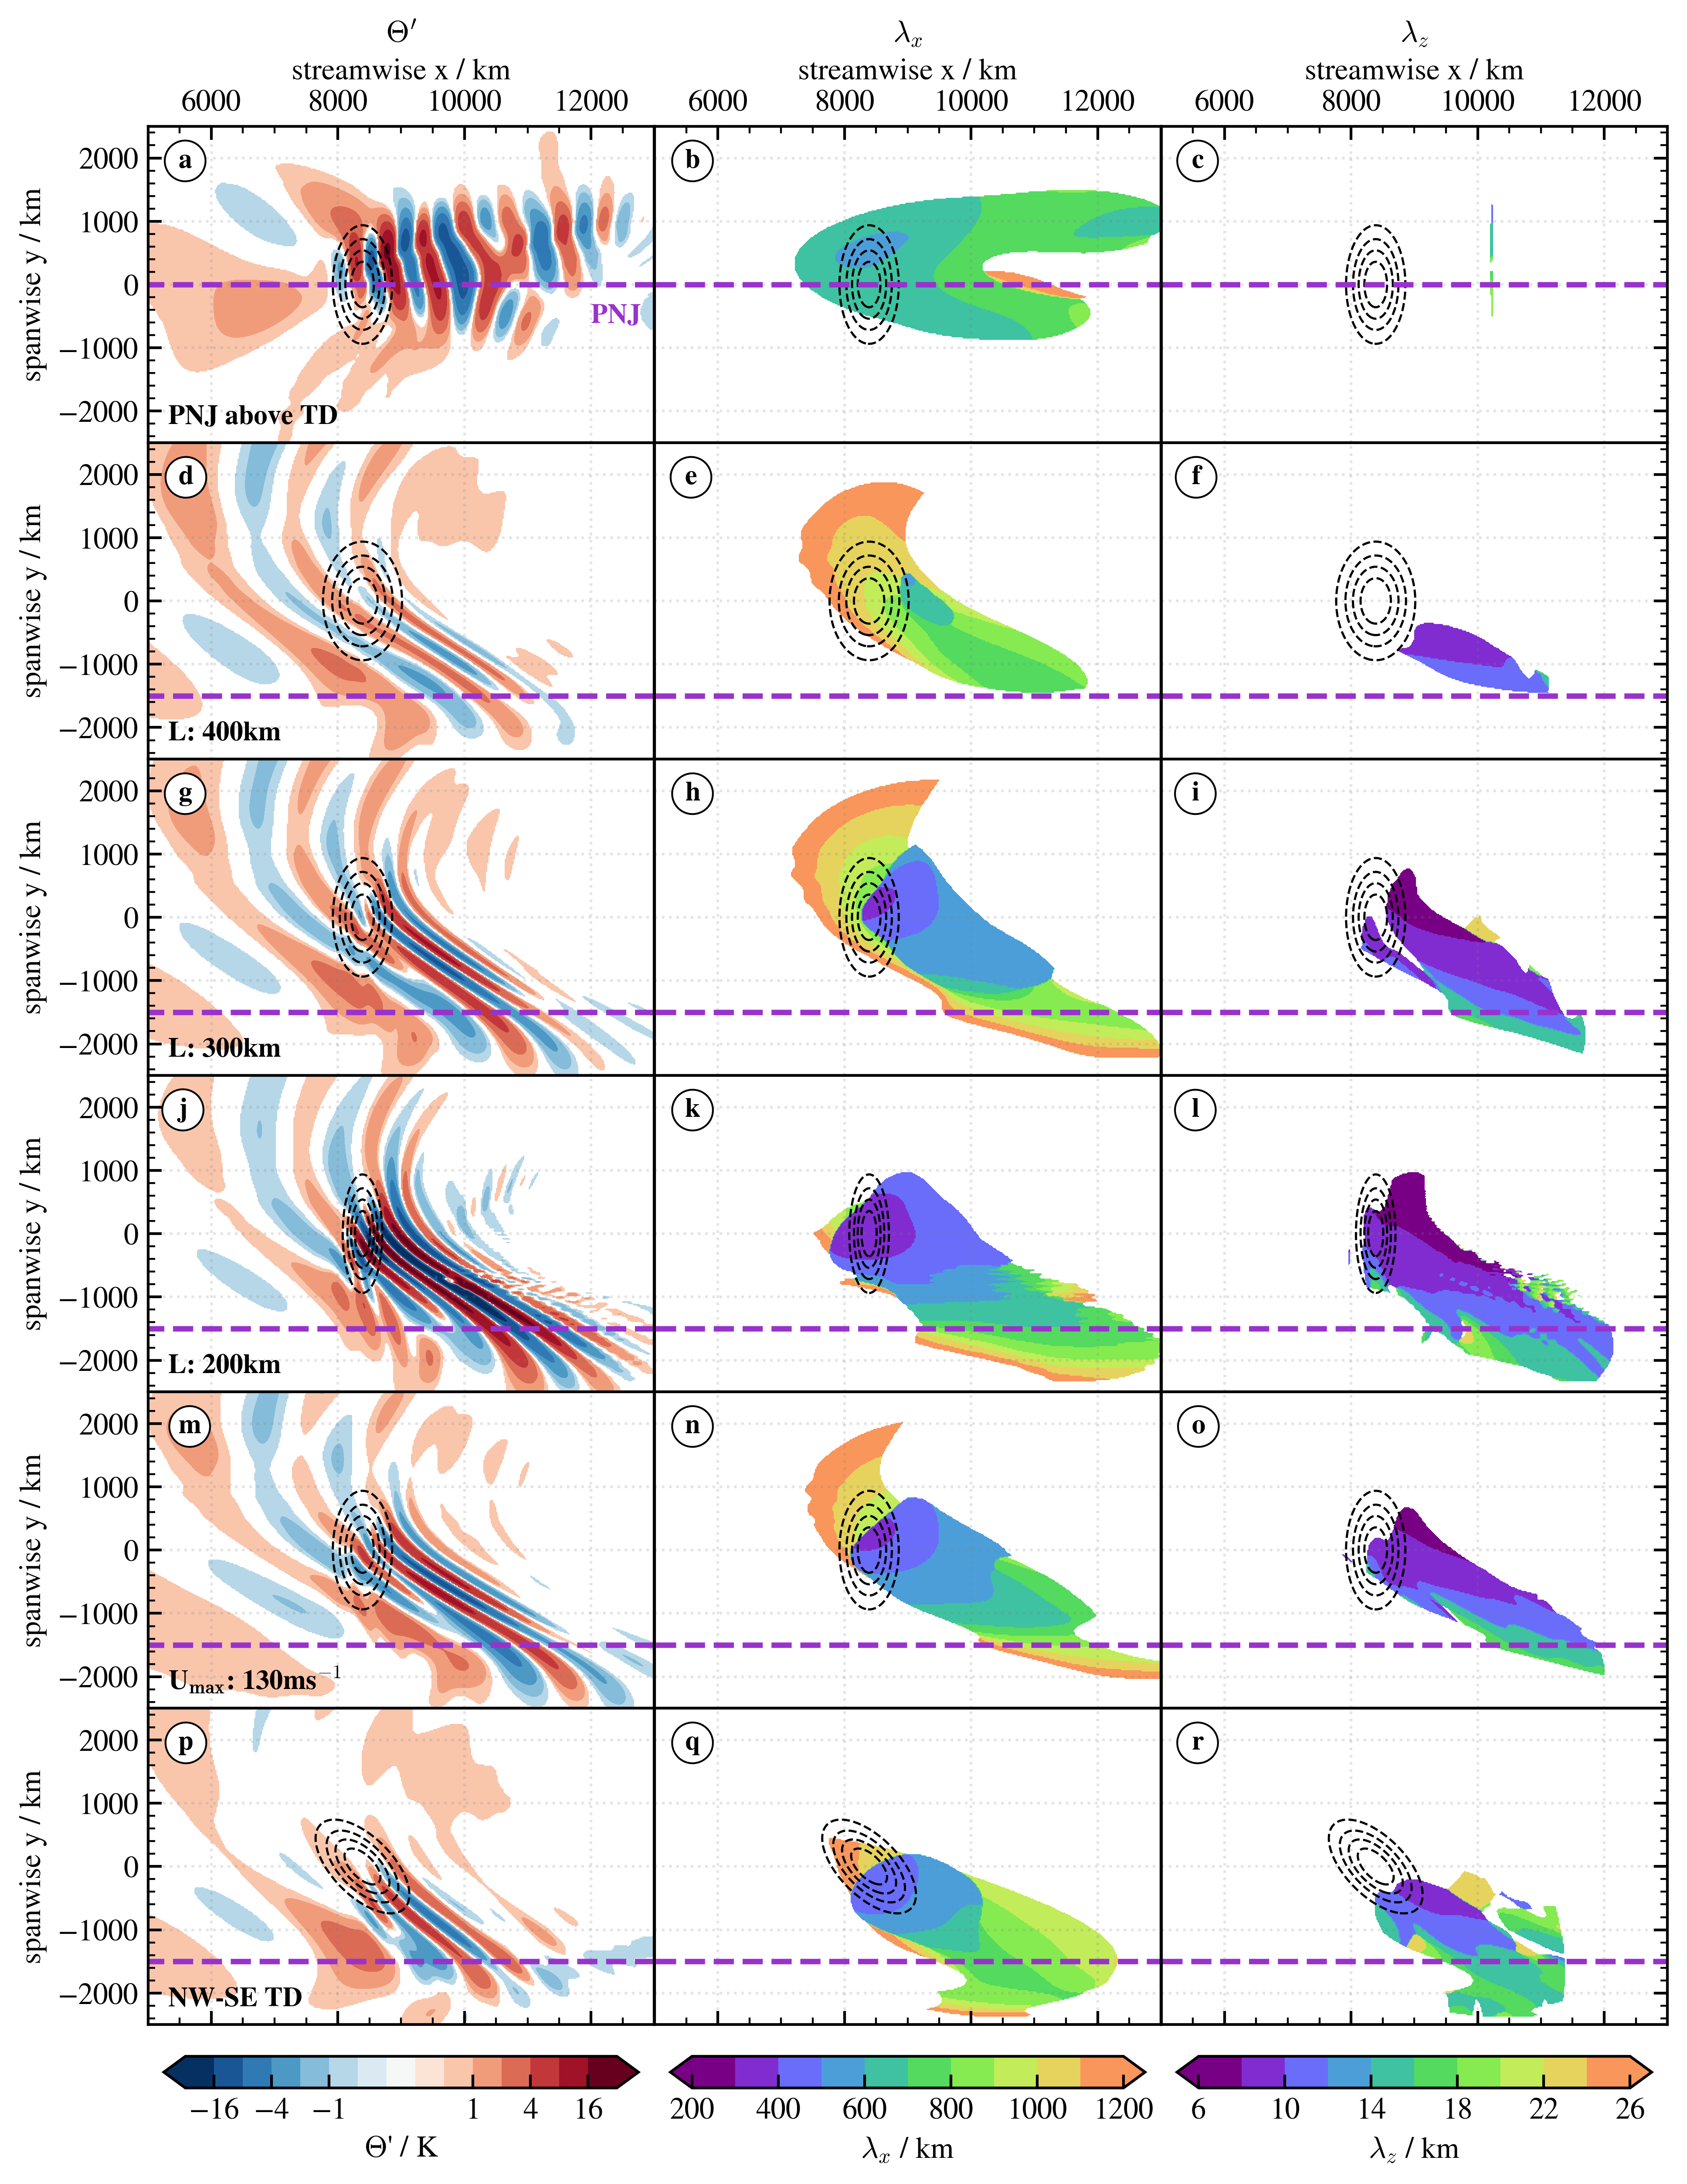
\includegraphics[width=0.99\textwidth]{figures_3D/waveletAna_overview.png}
    \caption{Similar cross sections as Figure \ref{fig:waveletAna}, but showing the zonal wavelength $\lambda_x$ in the second column and vertical wavelength $\lambda_z$ in the third column. The wavelenghts are based on a 1D wavelet analysis in each dimension.}
    \label{fig:waveletAna_xz}
\end{figure*}
%
\begin{figure*}[tbp]
    \centering
    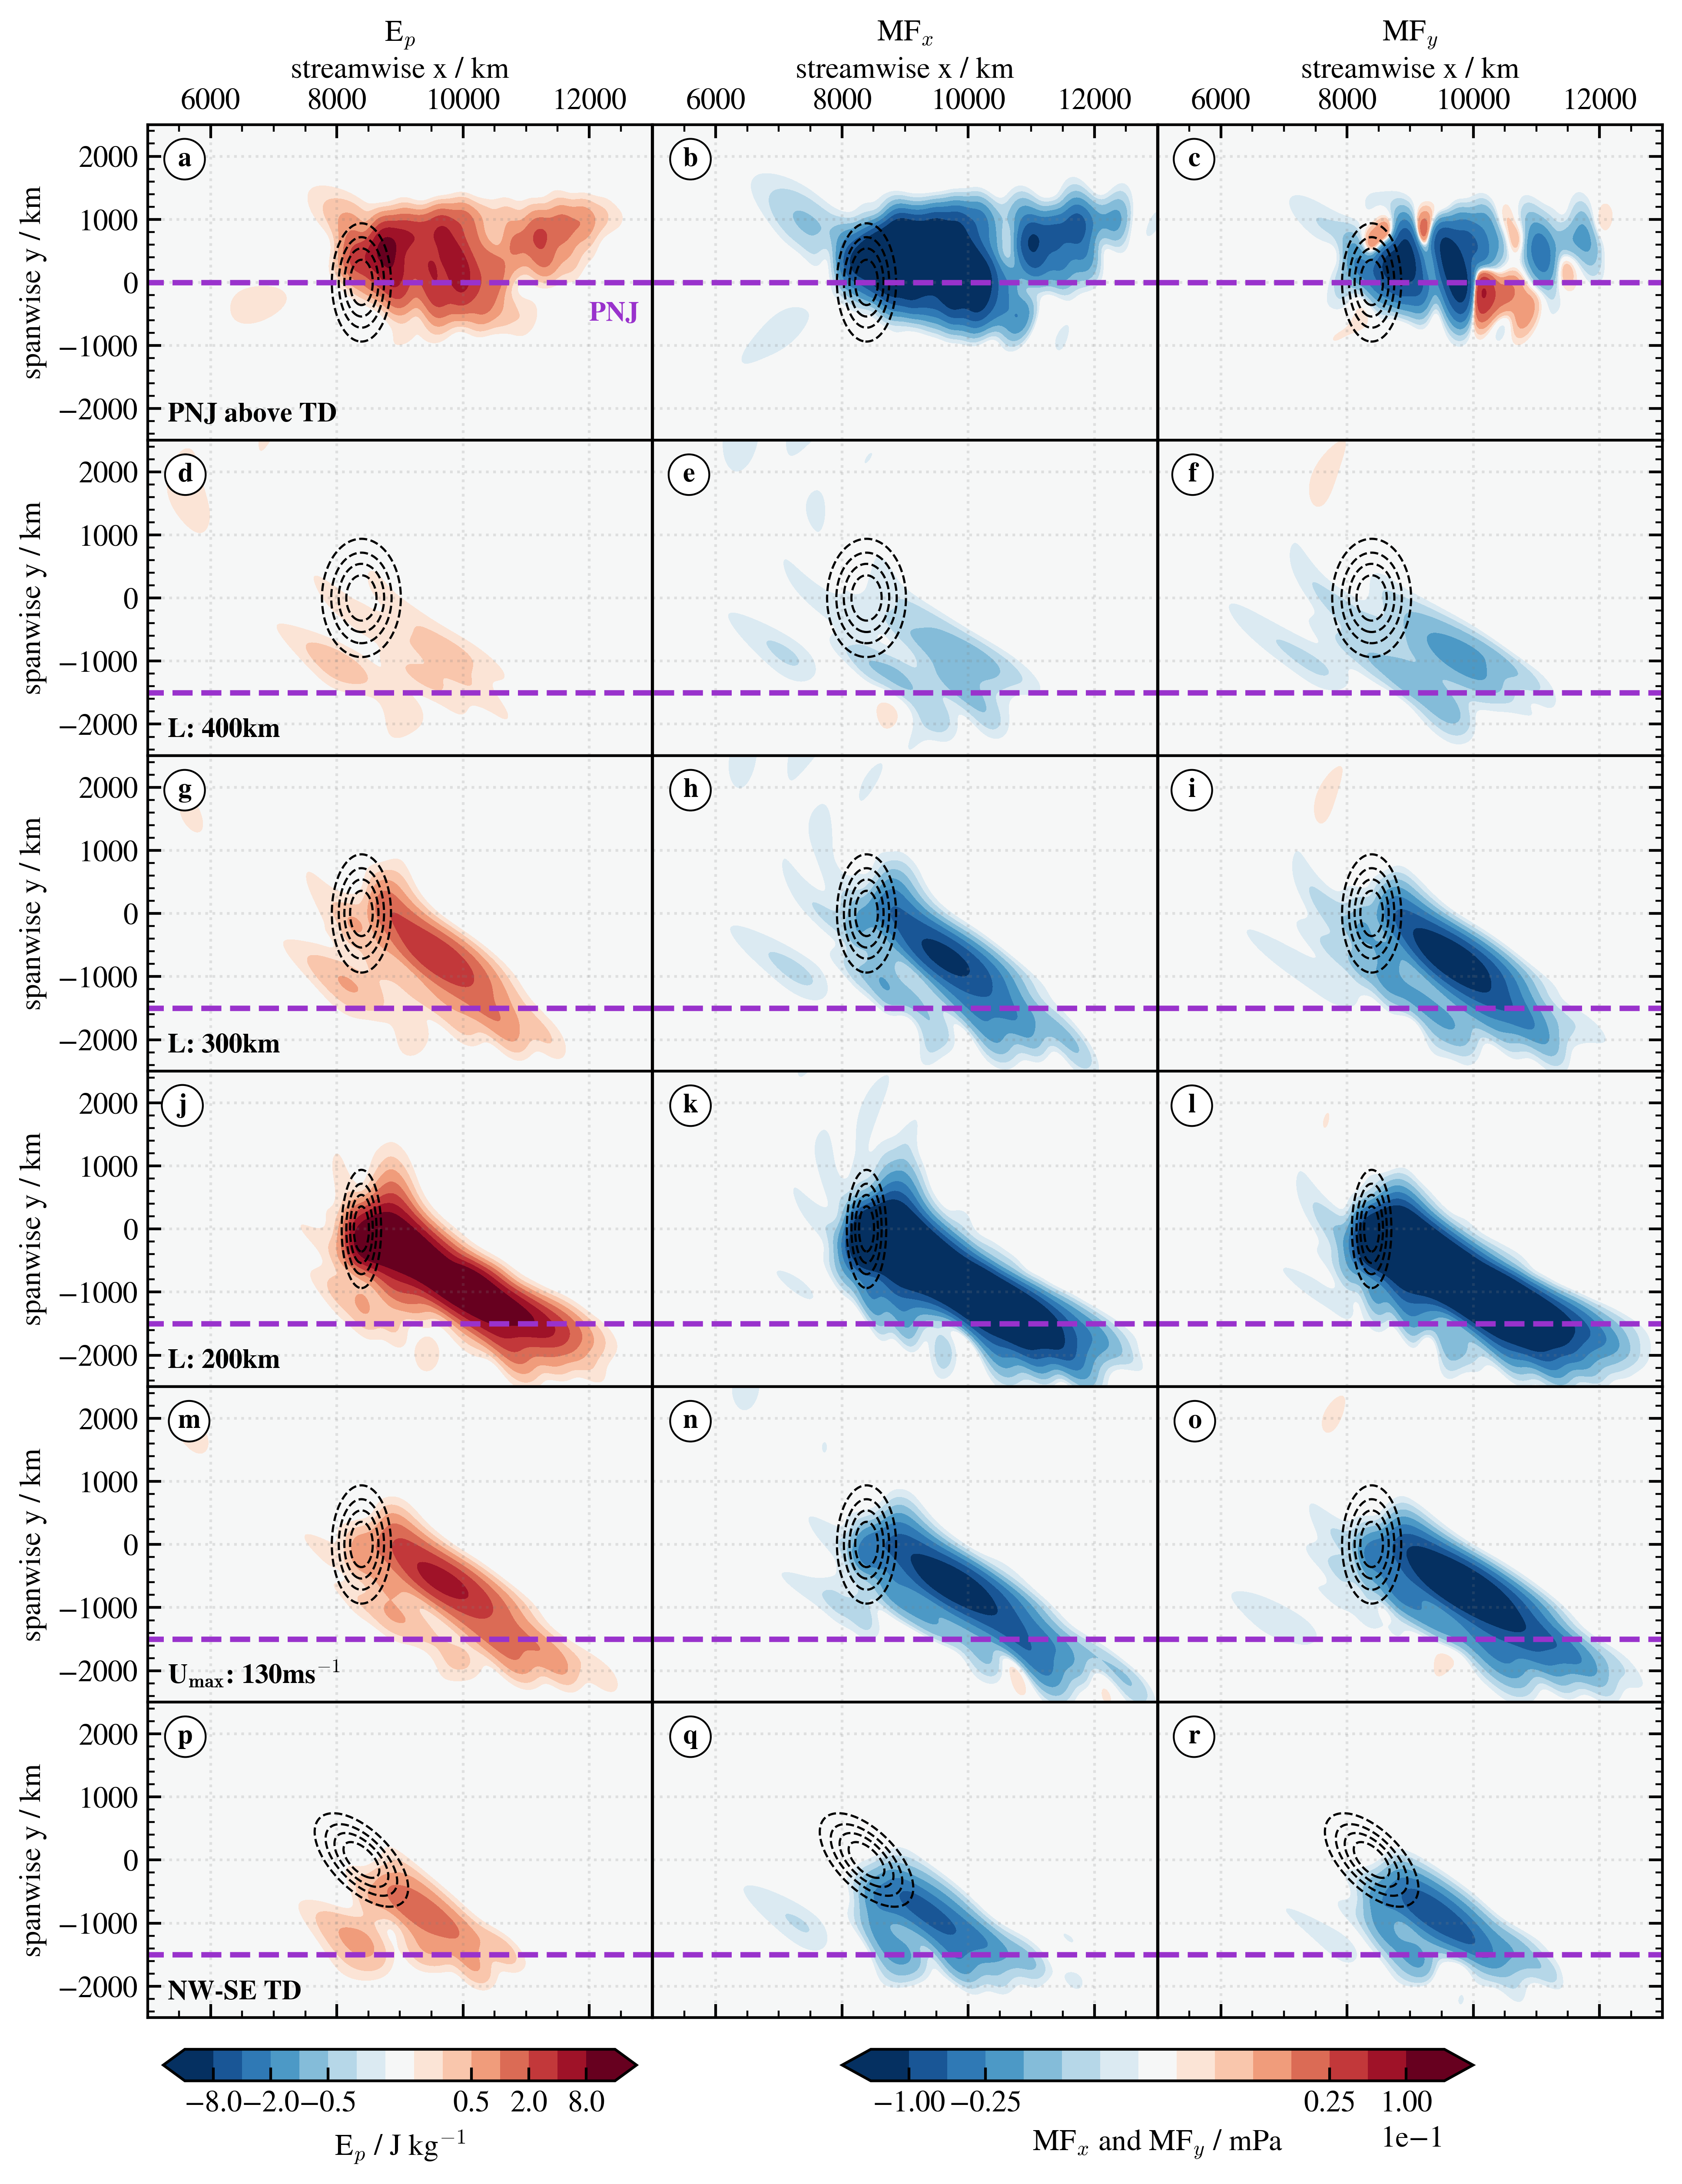
\includegraphics[width=0.99\textwidth]{figures_3D/waveletAna_mf.png}
    \caption{Similar cross sections as Figure \ref{fig:waveletAna}, but showing the potential energy E$_p$ in the first column, the zonal momentum flux MF$_x= \bar{\rho} \overbar{u'w'}$ in the second column and meridional momentum flux MF$_y= \bar{\rho} \overbar{v'w'}$ in the third column.}
    \label{fig:waveletAna_mf}
\end{figure*}
%
% Large quantities of data should be placed in an appendix. They should only be ``summarized'' in the chapter Results. Another way is to present some representative cases together with some extreme cases in the chapter Results. In any case, there should always appear a reference to the appendix in the main part of the thesis.
\newpage
\thispagestyle{plain}


% ==== START BACK MATTER (this has no visual effect)============================
\backmatter 

% ==== BIBLIOGRAPHY ============================================================
\printbibliography
\addcontentsline{toc}{chapter}{Bibliography}
% ---- use AMS reference format (use file ametsoc.bst included in ...
%      ... http://www.ametsoc.org/pubs/journals/AMS_Latex_V3.0.tar.gz):s
% \bibliographystyle{./ametsoc}   % ametsoc.bst in local directory
% ---- use BibTeX database file:
% \bibliography{./refs}      % mybibfile.bib in local directory
%\newpage
%\thispagestyle{plain}


% ==== ACKNOWLEDGMENTS =========================================================
% ---- include tex-file:
\chapter*{Acknowledgments}
\addcontentsline{toc}{chapter}{Acknowledgments}
\thispagestyle{plain}

I am deeply grateful for the patience and support of my supervisors, Andreas and Alexander. Thank you for being super flexible along the way, though this work took significantly longer than planned, and for investing your valuable time in discussions or correcting the thesis. I also want to thank Bernd Kaifler for providing the CORAL temperature measurements and the whole Middle Atmosphere group at the DLR for fruitful discussions and instructive inputs. The same applies to the numerical modeling group of Alexander Gohm at the University of Innsbruck.\\
I am grateful that the IPA, particularly Markus Rapp and Andreas Fix, gave me the opportunity to attend events like the SPARC Symposium in Frankfurt or the Southtrac-GW workshop in Bad Tölz. These have been exciting experiences.

At this point, I also want to thank the team of the avalanche warning service I worked with in between. Though snow at the surface and waves in the stratosphere do not have much in common, the methods we researchers use to analyze them all the more. Not only did I enjoy the time working there, the results and figures of my thesis also benefited from the interlude. Thank you, Machtl, for fun-filled evening coding sessions and for being an amazing wingman in and out of the office. And thank you, Christoph, for trusting us with awsome projects and being a great mentor.

My emotional thanks go to my family. You are my harbour when I make things too complicated from time to time. With you, life becomes easy again, and I am grateful I can always rely on you. And cheers, Valli, for being my favorite distraction while finishing this thesis.

% My emotional thanks go to my family, of course. Even though I rarely give the impression that I need help, I am grateful that I can always rely on you. 

% am very grateful that you gave me the opportunities to attend international conferences like the American and European Geoscience Unions and to do exciting trips to places like Kühlungsborn, Kiruna, S ̃ao José dos Campos or to the end of the world, Río Grande. 

% Thank you for your valuable time that you always in- vested in correcting my work. I assume it has not always been easy. Furthermore, I would like to thank the “Middle Atmosphere” matrix group at the IPA in Oberpfaffenhofen for countless discussions with colleagues such as Thomas Birner, Andreas Dörnbrack, Hella Garny, Sonja Gisinger, Stefanie Knobloch, Tyler Mixa and Henrike Willms. Thank you, Andreas, for taking me under your wings more and more during the course of my doctoral studies

% << Alex >>
% Now it is time to thank all people who have contributed to your work and who
% have supported you during your study. Do not forget to mention all relevant data
% providers and funding agencies (also provide the grant numbers).

%\newpage
%\thispagestyle{plain}


% ==== CURRICULUM VITAE ========================================================
% ---- include tex-file:
% \include{curricv}
% \newpage
% \thispagestyle{plain}


% ==== EPILOGUE ================================================================
% ---- include tex-file:
% \include{pre-and-post/epilogue}
% \newpage
% \thispagestyle{plain}


\end{document}
% ==== END OF BODY =============================================================
